\documentclass[a4paper]{book}
\usepackage{a4wide}
\usepackage{makeidx}
\usepackage{graphicx}
\usepackage{multicol}
\usepackage{float}
\usepackage{listings}
\usepackage{color}
\usepackage{textcomp}
\usepackage{alltt}
\usepackage{times}
\usepackage{ifpdf}
\ifpdf
\usepackage[pdftex,
            pagebackref=true,
            colorlinks=true,
            linkcolor=blue,
            unicode
           ]{hyperref}
\else
\usepackage[ps2pdf,
            pagebackref=true,
            colorlinks=true,
            linkcolor=blue,
            unicode
           ]{hyperref}
\usepackage{pspicture}
\fi
\usepackage[utf8]{inputenc}
\usepackage{doxygen}
\lstset{language=C++,inputencoding=utf8,basicstyle=\footnotesize,breaklines=true,breakatwhitespace=true,tabsize=8,numbers=left }
\makeindex
\setcounter{tocdepth}{3}
\renewcommand{\footrulewidth}{0.4pt}
\begin{document}
\hypersetup{pageanchor=false}
\begin{titlepage}
\vspace*{7cm}
\begin{center}
{\Large crml \\[1ex]\large .1 }\\
\vspace*{1cm}
{\large Generated by Doxygen 1.6.3}\\
\vspace*{0.5cm}
{\small Mon Nov 1 14:47:09 2010}\\
\end{center}
\end{titlepage}
\clearemptydoublepage
\pagenumbering{roman}
\tableofcontents
\clearemptydoublepage
\pagenumbering{arabic}
\hypersetup{pageanchor=true}
\chapter{Namespace Index}
\section{Namespace List}
Here is a list of all namespaces with brief descriptions:\begin{DoxyCompactList}
\item\contentsline{section}{\hyperlink{namespacebridge}{bridge} }{\pageref{namespacebridge}}{}
\item\contentsline{section}{\hyperlink{namespacecpplint}{cpplint} }{\pageref{namespacecpplint}}{}
\item\contentsline{section}{\hyperlink{namespacecrml}{crml} }{\pageref{namespacecrml}}{}
\item\contentsline{section}{\hyperlink{namespacehexdecode}{hexdecode} }{\pageref{namespacehexdecode}}{}
\item\contentsline{section}{\hyperlink{namespacehexencode}{hexencode} }{\pageref{namespacehexencode}}{}
\item\contentsline{section}{\hyperlink{namespacehexjs}{hexjs} }{\pageref{namespacehexjs}}{}
\item\contentsline{section}{\hyperlink{namespacehttpd}{httpd} }{\pageref{namespacehttpd}}{}
\item\contentsline{section}{\hyperlink{namespacepi__generator}{pi\_\-generator} }{\pageref{namespacepi__generator}}{}
\item\contentsline{section}{\hyperlink{namespacepp}{pp} }{\pageref{namespacepp}}{}
\item\contentsline{section}{\hyperlink{namespacescm}{scm} }{\pageref{namespacescm}}{}
\item\contentsline{section}{\hyperlink{namespaceshader__util}{shader\_\-util} }{\pageref{namespaceshader__util}}{}
\item\contentsline{section}{\hyperlink{namespacetransform__4x4}{transform\_\-4x4} }{\pageref{namespacetransform__4x4}}{}
\item\contentsline{section}{\hyperlink{namespacetumbler}{tumbler} }{\pageref{namespacetumbler}}{}
\end{DoxyCompactList}

\chapter{Class Index}
\section{Class Hierarchy}
This inheritance list is sorted roughly, but not completely, alphabetically:\begin{DoxyCompactList}
\item \contentsline{section}{scm::Clock}{\pageref{classscm_1_1_clock}}{}
\item \contentsline{section}{Context}{\pageref{struct_context}}{}
\item \contentsline{section}{crml::Core}{\pageref{classcrml_1_1_core}}{}
\item \contentsline{section}{tumbler::Cube}{\pageref{classtumbler_1_1_cube}}{}
\item \contentsline{section}{crml::Display}{\pageref{classcrml_1_1_display}}{}
\item \contentsline{section}{scm::Error}{\pageref{classscm_1_1_error}}{}
\begin{DoxyCompactList}
\item \contentsline{section}{scm::Event}{\pageref{classscm_1_1_event}}{}
\end{DoxyCompactList}
\item \contentsline{section}{EventHandler}{\pageref{class_event_handler}}{}
\item \contentsline{section}{HelloWorldInstance}{\pageref{class_hello_world_instance}}{}
\item \contentsline{section}{HelloWorldModule}{\pageref{class_hello_world_module}}{}
\item \contentsline{section}{HelloWorldScriptableObject}{\pageref{class_hello_world_scriptable_object}}{}
\item \contentsline{section}{scm::HexStore}{\pageref{classscm_1_1_hex_store}}{}
\item \contentsline{section}{MD5Digest\_\-struct}{\pageref{struct_m_d5_digest__struct}}{}
\item \contentsline{section}{pi\_\-generator::PiGenerator}{\pageref{classpi__generator_1_1_pi_generator}}{}
\item \contentsline{section}{httpd::QuittableHTTPHandler}{\pageref{classhttpd_1_1_quittable_h_t_t_p_handler}}{}
\item \contentsline{section}{httpd::QuittableHTTPServer}{\pageref{classhttpd_1_1_quittable_h_t_t_p_server}}{}
\item \contentsline{section}{ScriptingBridge}{\pageref{class_scripting_bridge}}{}
\item \contentsline{section}{bridge::ScriptingBridge}{\pageref{classbridge_1_1_scripting_bridge}}{}
\begin{DoxyCompactList}
\item \contentsline{section}{bridge::PiGenerator}{\pageref{classbridge_1_1_pi_generator}}{}
\end{DoxyCompactList}
\item \contentsline{section}{tumbler::ScriptingBridge}{\pageref{classtumbler_1_1_scripting_bridge}}{}
\item \contentsline{section}{pi\_\-generator::ScriptingBridge}{\pageref{classpi__generator_1_1_scripting_bridge}}{}
\item \contentsline{section}{TestObject}{\pageref{struct_test_object}}{}
\item \contentsline{section}{tumbler::Tumbler}{\pageref{classtumbler_1_1_tumbler}}{}
\item \contentsline{section}{tumbler::TumblerContext3D}{\pageref{structtumbler_1_1_tumbler_context3_d}}{}
\end{DoxyCompactList}

\chapter{Class Index}
\section{Class List}
Here are the classes, structs, unions and interfaces with brief descriptions:\begin{DoxyCompactList}
\item\contentsline{section}{\hyperlink{classscm_1_1_clock}{scm::Clock} }{\pageref{classscm_1_1_clock}}{}
\item\contentsline{section}{\hyperlink{struct_context}{Context} }{\pageref{struct_context}}{}
\item\contentsline{section}{\hyperlink{classcrml_1_1_core}{crml::Core} (The \hyperlink{classcrml_1_1_core}{Core} object which wires all subsystems and maintains an open channel with javascript )}{\pageref{classcrml_1_1_core}}{}
\item\contentsline{section}{\hyperlink{classtumbler_1_1_cube}{tumbler::Cube} }{\pageref{classtumbler_1_1_cube}}{}
\item\contentsline{section}{\hyperlink{classcrml_1_1_display}{crml::Display} }{\pageref{classcrml_1_1_display}}{}
\item\contentsline{section}{\hyperlink{classscm_1_1_error}{scm::Error} }{\pageref{classscm_1_1_error}}{}
\item\contentsline{section}{\hyperlink{classscm_1_1_event}{scm::Event} }{\pageref{classscm_1_1_event}}{}
\item\contentsline{section}{\hyperlink{class_event_handler}{EventHandler} }{\pageref{class_event_handler}}{}
\item\contentsline{section}{\hyperlink{class_hello_world_instance}{HelloWorldInstance} }{\pageref{class_hello_world_instance}}{}
\item\contentsline{section}{\hyperlink{class_hello_world_module}{HelloWorldModule} }{\pageref{class_hello_world_module}}{}
\item\contentsline{section}{\hyperlink{class_hello_world_scriptable_object}{HelloWorldScriptableObject} }{\pageref{class_hello_world_scriptable_object}}{}
\item\contentsline{section}{\hyperlink{classscm_1_1_hex_store}{scm::HexStore} }{\pageref{classscm_1_1_hex_store}}{}
\item\contentsline{section}{\hyperlink{struct_m_d5_digest__struct}{MD5Digest\_\-struct} }{\pageref{struct_m_d5_digest__struct}}{}
\item\contentsline{section}{\hyperlink{classbridge_1_1_pi_generator}{bridge::PiGenerator} }{\pageref{classbridge_1_1_pi_generator}}{}
\item\contentsline{section}{\hyperlink{classpi__generator_1_1_pi_generator}{pi\_\-generator::PiGenerator} }{\pageref{classpi__generator_1_1_pi_generator}}{}
\item\contentsline{section}{\hyperlink{classhttpd_1_1_quittable_h_t_t_p_handler}{httpd::QuittableHTTPHandler} }{\pageref{classhttpd_1_1_quittable_h_t_t_p_handler}}{}
\item\contentsline{section}{\hyperlink{classhttpd_1_1_quittable_h_t_t_p_server}{httpd::QuittableHTTPServer} }{\pageref{classhttpd_1_1_quittable_h_t_t_p_server}}{}
\item\contentsline{section}{\hyperlink{class_scripting_bridge}{ScriptingBridge} }{\pageref{class_scripting_bridge}}{}
\item\contentsline{section}{\hyperlink{classbridge_1_1_scripting_bridge}{bridge::ScriptingBridge} }{\pageref{classbridge_1_1_scripting_bridge}}{}
\item\contentsline{section}{\hyperlink{classtumbler_1_1_scripting_bridge}{tumbler::ScriptingBridge} }{\pageref{classtumbler_1_1_scripting_bridge}}{}
\item\contentsline{section}{\hyperlink{classpi__generator_1_1_scripting_bridge}{pi\_\-generator::ScriptingBridge} }{\pageref{classpi__generator_1_1_scripting_bridge}}{}
\item\contentsline{section}{\hyperlink{struct_test_object}{TestObject} }{\pageref{struct_test_object}}{}
\item\contentsline{section}{\hyperlink{classtumbler_1_1_tumbler}{tumbler::Tumbler} }{\pageref{classtumbler_1_1_tumbler}}{}
\item\contentsline{section}{\hyperlink{structtumbler_1_1_tumbler_context3_d}{tumbler::TumblerContext3D} }{\pageref{structtumbler_1_1_tumbler_context3_d}}{}
\end{DoxyCompactList}

\chapter{File Index}
\section{File List}
Here is a list of all files with brief descriptions:\begin{DoxyCompactList}
\item\contentsline{section}{/home/derek/dev/crml/crml/lib/tumbler/\hyperlink{basic__macros_8h}{basic\_\-macros.h} }{\pageref{basic__macros_8h}}{}
\item\contentsline{section}{/home/derek/dev/crml/crml/lib/tumbler/\hyperlink{cube_8cc}{cube.cc} }{\pageref{cube_8cc}}{}
\item\contentsline{section}{/home/derek/dev/crml/crml/lib/tumbler/\hyperlink{cube_8h}{cube.h} }{\pageref{cube_8h}}{}
\item\contentsline{section}{/home/derek/dev/crml/crml/lib/tumbler/\hyperlink{lib_2tumbler_2npn__bridge_8cc}{npn\_\-bridge.cc} }{\pageref{lib_2tumbler_2npn__bridge_8cc}}{}
\item\contentsline{section}{/home/derek/dev/crml/crml/lib/tumbler/\hyperlink{lib_2tumbler_2npp__gate_8cc}{npp\_\-gate.cc} }{\pageref{lib_2tumbler_2npp__gate_8cc}}{}
\item\contentsline{section}{/home/derek/dev/crml/crml/lib/tumbler/\hyperlink{lib_2tumbler_2scripting__bridge_8cc}{scripting\_\-bridge.cc} }{\pageref{lib_2tumbler_2scripting__bridge_8cc}}{}
\item\contentsline{section}{/home/derek/dev/crml/crml/lib/tumbler/\hyperlink{lib_2tumbler_2scripting__bridge_8h}{scripting\_\-bridge.h} }{\pageref{lib_2tumbler_2scripting__bridge_8h}}{}
\item\contentsline{section}{/home/derek/dev/crml/crml/lib/tumbler/\hyperlink{shader__util_8cc}{shader\_\-util.cc} }{\pageref{shader__util_8cc}}{}
\item\contentsline{section}{/home/derek/dev/crml/crml/lib/tumbler/\hyperlink{shader__util_8h}{shader\_\-util.h} }{\pageref{shader__util_8h}}{}
\item\contentsline{section}{/home/derek/dev/crml/crml/lib/tumbler/\hyperlink{transforms_8cc}{transforms.cc} }{\pageref{transforms_8cc}}{}
\item\contentsline{section}{/home/derek/dev/crml/crml/lib/tumbler/\hyperlink{transforms_8h}{transforms.h} }{\pageref{transforms_8h}}{}
\item\contentsline{section}{/home/derek/dev/crml/crml/lib/tumbler/\hyperlink{tumbler_8cc}{tumbler.cc} }{\pageref{tumbler_8cc}}{}
\item\contentsline{section}{/home/derek/dev/crml/crml/lib/tumbler/\hyperlink{tumbler_8h}{tumbler.h} }{\pageref{tumbler_8h}}{}
\item\contentsline{section}{/home/derek/dev/crml/crml/lib/tumbler/\hyperlink{tumbler__module_8cc}{tumbler\_\-module.cc} }{\pageref{tumbler__module_8cc}}{}
\item\contentsline{section}{/home/derek/dev/crml/crml/src/core/\hyperlink{core_8h}{core.h} }{\pageref{core_8h}}{}
\item\contentsline{section}{/home/derek/dev/crml/crml/src/core/\hyperlink{src_2core_2npn__bridge_8cc}{npn\_\-bridge.cc} }{\pageref{src_2core_2npn__bridge_8cc}}{}
\item\contentsline{section}{/home/derek/dev/crml/crml/src/core/\hyperlink{src_2core_2npp__gate_8cc}{npp\_\-gate.cc} }{\pageref{src_2core_2npp__gate_8cc}}{}
\item\contentsline{section}{/home/derek/dev/crml/crml/src/core/\hyperlink{src_2core_2scripting__bridge_8cc}{scripting\_\-bridge.cc} }{\pageref{src_2core_2scripting__bridge_8cc}}{}
\item\contentsline{section}{/home/derek/dev/crml/crml/src/core/\hyperlink{src_2core_2scripting__bridge_8h}{scripting\_\-bridge.h} }{\pageref{src_2core_2scripting__bridge_8h}}{}
\item\contentsline{section}{/home/derek/dev/crml/crml/src/evt/\hyperlink{event_8cc}{event.cc} }{\pageref{event_8cc}}{}
\item\contentsline{section}{/home/derek/dev/crml/crml/src/evt/\hyperlink{event_8h}{event.h} }{\pageref{event_8h}}{}
\item\contentsline{section}{/home/derek/dev/crml/crml/src/evt/\hyperlink{event__handler_8cc}{event\_\-handler.cc} }{\pageref{event__handler_8cc}}{}
\item\contentsline{section}{/home/derek/dev/crml/crml/src/evt/\hyperlink{event__handler_8h}{event\_\-handler.h} }{\pageref{event__handler_8h}}{}
\item\contentsline{section}{/home/derek/dev/crml/crml/src/gfx/\hyperlink{display_8hpp}{display.hpp} }{\pageref{display_8hpp}}{}
\item\contentsline{section}{/home/derek/dev/crml/crml/src/gfx/\hyperlink{gles2__demo__cc_8cc}{gles2\_\-demo\_\-cc.cc} }{\pageref{gles2__demo__cc_8cc}}{}
\item\contentsline{section}{/home/derek/dev/crml/crml/src/gfx/\hyperlink{gles2__demo__cc_8h}{gles2\_\-demo\_\-cc.h} }{\pageref{gles2__demo__cc_8h}}{}
\item\contentsline{section}{/home/derek/dev/crml/crml/src/gfx/\hyperlink{_png_image_8h}{PngImage.h} }{\pageref{_png_image_8h}}{}
\item\contentsline{section}{/home/derek/dev/crml/crml/src/include/\hyperlink{crml-aud_8h}{crml-\/aud.h} }{\pageref{crml-aud_8h}}{}
\item\contentsline{section}{/home/derek/dev/crml/crml/src/include/\hyperlink{crml-core_8h}{crml-\/core.h} }{\pageref{crml-core_8h}}{}
\item\contentsline{section}{/home/derek/dev/crml/crml/src/include/\hyperlink{crml-evt_8h}{crml-\/evt.h} }{\pageref{crml-evt_8h}}{}
\item\contentsline{section}{/home/derek/dev/crml/crml/src/include/\hyperlink{crml-gfx_8h}{crml-\/gfx.h} }{\pageref{crml-gfx_8h}}{}
\item\contentsline{section}{/home/derek/dev/crml/crml/src/include/\hyperlink{crml-net_8h}{crml-\/net.h} }{\pageref{crml-net_8h}}{}
\item\contentsline{section}{/home/derek/dev/crml/crml/src/include/\hyperlink{crml-sys_8h}{crml-\/sys.h} }{\pageref{crml-sys_8h}}{}
\item\contentsline{section}{/home/derek/dev/crml/crml/src/include/\hyperlink{crml-util_8h}{crml-\/util.h} }{\pageref{crml-util_8h}}{}
\item\contentsline{section}{/home/derek/dev/crml/crml/src/include/\hyperlink{crml-web_8h}{crml-\/web.h} }{\pageref{crml-web_8h}}{}
\item\contentsline{section}{/home/derek/dev/crml/crml/src/include/\hyperlink{crml-win_8h}{crml-\/win.h} }{\pageref{crml-win_8h}}{}
\item\contentsline{section}{/home/derek/dev/crml/crml/src/sys/\hyperlink{clock_8cc}{clock.cc} }{\pageref{clock_8cc}}{}
\item\contentsline{section}{/home/derek/dev/crml/crml/src/sys/\hyperlink{clock_8h}{clock.h} }{\pageref{clock_8h}}{}
\item\contentsline{section}{/home/derek/dev/crml/crml/src/sys/\hyperlink{error_8cc}{error.cc} }{\pageref{error_8cc}}{}
\item\contentsline{section}{/home/derek/dev/crml/crml/src/sys/\hyperlink{error_8h}{error.h} }{\pageref{error_8h}}{}
\item\contentsline{section}{/home/derek/dev/crml/crml/src/sys/\hyperlink{error__macro_8cc}{error\_\-macro.cc} }{\pageref{error__macro_8cc}}{}
\item\contentsline{section}{/home/derek/dev/crml/crml/src/sys/\hyperlink{hex__store_8cc}{hex\_\-store.cc} }{\pageref{hex__store_8cc}}{}
\item\contentsline{section}{/home/derek/dev/crml/crml/src/sys/\hyperlink{hex__store_8h}{hex\_\-store.h} }{\pageref{hex__store_8h}}{}
\item\contentsline{section}{/home/derek/dev/crml/crml/src/sys/\hyperlink{hexdecode_8cc}{hexdecode.cc} }{\pageref{hexdecode_8cc}}{}
\item\contentsline{section}{/home/derek/dev/crml/crml/src/sys/\hyperlink{log__macro_8cc}{log\_\-macro.cc} }{\pageref{log__macro_8cc}}{}
\item\contentsline{section}{/home/derek/dev/crml/crml/src/sys/\hyperlink{md5_8cc}{md5.cc} }{\pageref{md5_8cc}}{}
\item\contentsline{section}{/home/derek/dev/crml/crml/src/sys/\hyperlink{md5_8h}{md5.h} }{\pageref{md5_8h}}{}
\item\contentsline{section}{/home/derek/dev/crml/crml/src/sys/\hyperlink{src_2sys_2scripting__bridge_8h}{scripting\_\-bridge.h} }{\pageref{src_2sys_2scripting__bridge_8h}}{}
\item\contentsline{section}{/home/derek/dev/crml/crml/src/sys/tmp/\hyperlink{jslog_8cc}{jslog.cc} }{\pageref{jslog_8cc}}{}
\item\contentsline{section}{/home/derek/dev/crml/crml/src/web/\hyperlink{src_2web_2httpd_8py}{httpd.py} }{\pageref{src_2web_2httpd_8py}}{}
\item\contentsline{section}{/home/derek/dev/crml/crml/test/\hyperlink{hexjs_8py}{hexjs.py} }{\pageref{hexjs_8py}}{}
\item\contentsline{section}{/home/derek/dev/crml/crml/test/\hyperlink{test_2httpd_8py}{httpd.py} }{\pageref{test_2httpd_8py}}{}
\item\contentsline{section}{/home/derek/dev/crml/crml/test/\hyperlink{test-clock_8cc}{test-\/clock.cc} }{\pageref{test-clock_8cc}}{}
\item\contentsline{section}{/home/derek/dev/crml/crml/test/\hyperlink{test-macros_8cc}{test-\/macros.cc} }{\pageref{test-macros_8cc}}{}
\item\contentsline{section}{/home/derek/dev/crml/crml/test/\hyperlink{test-point_8cc}{test-\/point.cc} }{\pageref{test-point_8cc}}{}
\item\contentsline{section}{/home/derek/dev/crml/crml/test/\hyperlink{test__object_8cc}{test\_\-object.cc} }{\pageref{test__object_8cc}}{}
\item\contentsline{section}{/home/derek/dev/crml/crml/test/\hyperlink{test__object_8h}{test\_\-object.h} }{\pageref{test__object_8h}}{}
\item\contentsline{section}{/home/derek/dev/crml/crml/test/crml\_\-hello\_\-world/\hyperlink{test_2crml__hello__world_2npn__bridge_8cc}{npn\_\-bridge.cc} }{\pageref{test_2crml__hello__world_2npn__bridge_8cc}}{}
\item\contentsline{section}{/home/derek/dev/crml/crml/test/crml\_\-hello\_\-world/\hyperlink{test_2crml__hello__world_2npp__gate_8cc}{npp\_\-gate.cc} }{\pageref{test_2crml__hello__world_2npp__gate_8cc}}{}
\item\contentsline{section}{/home/derek/dev/crml/crml/test/crml\_\-hello\_\-world/\hyperlink{crml__hello__world_2pi__generator_8cc}{pi\_\-generator.cc} }{\pageref{crml__hello__world_2pi__generator_8cc}}{}
\item\contentsline{section}{/home/derek/dev/crml/crml/test/crml\_\-hello\_\-world/\hyperlink{crml__hello__world_2pi__generator_8h}{pi\_\-generator.h} }{\pageref{crml__hello__world_2pi__generator_8h}}{}
\item\contentsline{section}{/home/derek/dev/crml/crml/test/crml\_\-hello\_\-world/\hyperlink{crml__hello__world_2pi__generator__module_8cc}{pi\_\-generator\_\-module.cc} }{\pageref{crml__hello__world_2pi__generator__module_8cc}}{}
\item\contentsline{section}{/home/derek/dev/crml/crml/test/crml\_\-hello\_\-world/\hyperlink{test_2crml__hello__world_2scripting__bridge_8cc}{scripting\_\-bridge.cc} }{\pageref{test_2crml__hello__world_2scripting__bridge_8cc}}{}
\item\contentsline{section}{/home/derek/dev/crml/crml/test/crml\_\-hello\_\-world/\hyperlink{test_2crml__hello__world_2scripting__bridge_8h}{scripting\_\-bridge.h} }{\pageref{test_2crml__hello__world_2scripting__bridge_8h}}{}
\item\contentsline{section}{/home/derek/dev/crml/crml/test/hello\_\-world/\hyperlink{hello__world_8cc}{hello\_\-world.cc} }{\pageref{hello__world_8cc}}{}
\item\contentsline{section}{/home/derek/dev/crml/crml/test/pi\_\-generator/\hyperlink{test_2pi__generator_2npn__bridge_8cc}{npn\_\-bridge.cc} }{\pageref{test_2pi__generator_2npn__bridge_8cc}}{}
\item\contentsline{section}{/home/derek/dev/crml/crml/test/pi\_\-generator/\hyperlink{npn__bridge_8cc_8_b_a_c_k_u_p_828061_8cc}{npn\_\-bridge.cc.BACKUP.28061.cc} }{\pageref{npn__bridge_8cc_8_b_a_c_k_u_p_828061_8cc}}{}
\item\contentsline{section}{/home/derek/dev/crml/crml/test/pi\_\-generator/\hyperlink{npn__bridge_8cc_8_l_o_c_a_l_828061_8cc}{npn\_\-bridge.cc.LOCAL.28061.cc} }{\pageref{npn__bridge_8cc_8_l_o_c_a_l_828061_8cc}}{}
\item\contentsline{section}{/home/derek/dev/crml/crml/test/pi\_\-generator/\hyperlink{npn__bridge_8cc_8_r_e_m_o_t_e_828061_8cc}{npn\_\-bridge.cc.REMOTE.28061.cc} }{\pageref{npn__bridge_8cc_8_r_e_m_o_t_e_828061_8cc}}{}
\item\contentsline{section}{/home/derek/dev/crml/crml/test/pi\_\-generator/\hyperlink{test_2pi__generator_2npp__gate_8cc}{npp\_\-gate.cc} }{\pageref{test_2pi__generator_2npp__gate_8cc}}{}
\item\contentsline{section}{/home/derek/dev/crml/crml/test/pi\_\-generator/\hyperlink{pi__generator_2pi__generator_8cc}{pi\_\-generator.cc} }{\pageref{pi__generator_2pi__generator_8cc}}{}
\item\contentsline{section}{/home/derek/dev/crml/crml/test/pi\_\-generator/\hyperlink{pi__generator_2pi__generator_8h}{pi\_\-generator.h} }{\pageref{pi__generator_2pi__generator_8h}}{}
\item\contentsline{section}{/home/derek/dev/crml/crml/test/pi\_\-generator/\hyperlink{pi__generator_2pi__generator__module_8cc}{pi\_\-generator\_\-module.cc} }{\pageref{pi__generator_2pi__generator__module_8cc}}{}
\item\contentsline{section}{/home/derek/dev/crml/crml/test/pi\_\-generator/\hyperlink{test_2pi__generator_2scripting__bridge_8cc}{scripting\_\-bridge.cc} }{\pageref{test_2pi__generator_2scripting__bridge_8cc}}{}
\item\contentsline{section}{/home/derek/dev/crml/crml/test/pi\_\-generator/\hyperlink{test_2pi__generator_2scripting__bridge_8h}{scripting\_\-bridge.h} }{\pageref{test_2pi__generator_2scripting__bridge_8h}}{}
\item\contentsline{section}{/home/derek/dev/crml/crml/test/pi\_\-generator\_\-crml/\hyperlink{test_2pi__generator__crml_2npp__gate_8cc}{npp\_\-gate.cc} }{\pageref{test_2pi__generator__crml_2npp__gate_8cc}}{}
\item\contentsline{section}{/home/derek/dev/crml/crml/test/pi\_\-generator\_\-crml/\hyperlink{pi__generator__crml_2pi__generator_8cc}{pi\_\-generator.cc} }{\pageref{pi__generator__crml_2pi__generator_8cc}}{}
\item\contentsline{section}{/home/derek/dev/crml/crml/test/pi\_\-generator\_\-crml/\hyperlink{pi__generator__crml_2pi__generator_8h}{pi\_\-generator.h} }{\pageref{pi__generator__crml_2pi__generator_8h}}{}
\item\contentsline{section}{/home/derek/dev/crml/crml/test/pi\_\-generator\_\-crml/\hyperlink{pi__generator__crml_2pi__generator__module_8cc}{pi\_\-generator\_\-module.cc} }{\pageref{pi__generator__crml_2pi__generator__module_8cc}}{}
\item\contentsline{section}{/home/derek/dev/crml/crml/test/pi\_\-generator\_\-crml/old/\hyperlink{test_2pi__generator__crml_2old_2npn__bridge_8cc}{npn\_\-bridge.cc} }{\pageref{test_2pi__generator__crml_2old_2npn__bridge_8cc}}{}
\item\contentsline{section}{/home/derek/dev/crml/crml/test/pi\_\-generator\_\-crml/old/\hyperlink{test_2pi__generator__crml_2old_2scripting__bridge_8cc}{scripting\_\-bridge.cc} }{\pageref{test_2pi__generator__crml_2old_2scripting__bridge_8cc}}{}
\item\contentsline{section}{/home/derek/dev/crml/crml/test/pi\_\-generator\_\-crml/old/\hyperlink{test_2pi__generator__crml_2old_2scripting__bridge_8h}{scripting\_\-bridge.h} }{\pageref{test_2pi__generator__crml_2old_2scripting__bridge_8h}}{}
\item\contentsline{section}{/home/derek/dev/crml/crml/tools/\hyperlink{cpplint_8py}{cpplint.py} }{\pageref{cpplint_8py}}{}
\item\contentsline{section}{/home/derek/dev/crml/crml/tools/\hyperlink{hexdecode_8py}{hexdecode.py} }{\pageref{hexdecode_8py}}{}
\item\contentsline{section}{/home/derek/dev/crml/crml/tools/\hyperlink{hexencode_8py}{hexencode.py} }{\pageref{hexencode_8py}}{}
\end{DoxyCompactList}

\chapter{Namespace Documentation}
\hypertarget{namespacecpplint}{
\section{cpplint Namespace Reference}
\label{namespacecpplint}\index{cpplint@{cpplint}}
}
\subsection*{Functions}
\begin{DoxyCompactItemize}
\item 
def \hyperlink{namespacecpplint_a9713059a1f275ecb548f18733306791d}{CloseExpression}
\item 
def \hyperlink{namespacecpplint_ac9cdecc582bc833c2eb7ac6eed6d2624}{CheckForCopyright}
\item 
def \hyperlink{namespacecpplint_a8eedb7313093d59b41bd7c5b19c2ddaf}{GetHeaderGuardCPPVariable}
\item 
def \hyperlink{namespacecpplint_a6ecd551d11dde0a916ef4a6317b70585}{CheckForHeaderGuard}
\item 
def \hyperlink{namespacecpplint_a04dd8f7483533a2ec7df687c180e9d22}{CheckForUnicodeReplacementCharacters}
\item 
def \hyperlink{namespacecpplint_a84408591ac7ff7e427560a252360070b}{CheckForNewlineAtEOF}
\item 
def \hyperlink{namespacecpplint_ae319b3dce42ad005bcddfd3d4df9656d}{CheckForMultilineCommentsAndStrings}
\end{DoxyCompactItemize}
\subsection*{Variables}
\begin{DoxyCompactItemize}
\item 
string \hyperlink{namespacecpplint_afefe1ab8eeab7350e1a7d96d41c86fb8}{\_\-USAGE}
\item 
list \hyperlink{namespacecpplint_a7a498bc09903cee9029cccc023641ede}{\_\-ERROR\_\-CATEGORIES}
\item 
list \hyperlink{namespacecpplint_a40307223380a2e065996f7113e2f8f4c}{\_\-DEFAULT\_\-FILTERS} = \mbox{[} '-\/build/include\_\-alpha' \mbox{]}
\item 
tuple \hyperlink{namespacecpplint_a76f8ec9e9e1ea46197f611bd5a995962}{\_\-STL\_\-HEADERS}
\item 
tuple \hyperlink{namespacecpplint_a8b16f3827d7722217dd3a2f50f24087d}{\_\-CPP\_\-HEADERS}
\item 
list \hyperlink{namespacecpplint_aab5915e25e8ef5ed9d9c223a5183d6bc}{\_\-CHECK\_\-MACROS}
\item 
tuple \hyperlink{namespacecpplint_ad966b15edc61d0e0fa98cf4ce1a0135a}{\_\-CHECK\_\-REPLACEMENT} = dict(\mbox{[}(m, \{\}) for m in \hyperlink{namespacecpplint_aab5915e25e8ef5ed9d9c223a5183d6bc}{\_\-CHECK\_\-MACROS}\mbox{]})
\item 
int \hyperlink{namespacecpplint_a6703b407df0f07ff6162c225070ddc9e}{\_\-C\_\-SYS\_\-HEADER} = 1
\item 
int \hyperlink{namespacecpplint_a89c3b71932122fc90afd2f47c07574f4}{\_\-CPP\_\-SYS\_\-HEADER} = 2
\item 
int \hyperlink{namespacecpplint_a5d6aba92ab2575ff645a1aacad5b5216}{\_\-LIKELY\_\-MY\_\-HEADER} = 3
\item 
int \hyperlink{namespacecpplint_a40cf12907322271bf94416a9fe602d96}{\_\-POSSIBLE\_\-MY\_\-HEADER} = 4
\item 
int \hyperlink{namespacecpplint_ace812856f1cd6c6b4375ab5c92294323}{\_\-OTHER\_\-HEADER} = 5
\item 
dictionary \hyperlink{namespacecpplint_a3eea0656ee957fff7d4511579c92d250}{\_\-regexp\_\-compile\_\-cache} = \{\}
\item 
tuple \hyperlink{namespacecpplint_af6a02614cf018ab890ede0b3a936ba6e}{\_\-RE\_\-SUPPRESSION} = re.compile(r'$\backslash$bNOLINT$\backslash$b($\backslash$(\mbox{[}$^\wedge$)\mbox{]}$\ast$$\backslash$))
\item 
tuple \hyperlink{namespacecpplint_a8559d5bdf881337b323a7253a71a5fed}{elided} = \_\-RE\_\-PATTERN\_\-CLEANSE\_\-LINE\_\-ESCAPES.sub('', \hyperlink{namespacecpplint_a8559d5bdf881337b323a7253a71a5fed}{elided})
\end{DoxyCompactItemize}


\subsection{Function Documentation}
\hypertarget{namespacecpplint_ac9cdecc582bc833c2eb7ac6eed6d2624}{
\index{cpplint@{cpplint}!CheckForCopyright@{CheckForCopyright}}
\index{CheckForCopyright@{CheckForCopyright}!cpplint@{cpplint}}
\subsubsection[{CheckForCopyright}]{\setlength{\rightskip}{0pt plus 5cm}def cpplint::CheckForCopyright ( {\em filename}, \/   {\em lines}, \/   {\em error})}}
\label{namespacecpplint_ac9cdecc582bc833c2eb7ac6eed6d2624}
\begin{DoxyVerb}Logs an error if no Copyright message appears at the top of the file.\end{DoxyVerb}
 

Definition at line 1005 of file cpplint.py.

\hypertarget{namespacecpplint_a6ecd551d11dde0a916ef4a6317b70585}{
\index{cpplint@{cpplint}!CheckForHeaderGuard@{CheckForHeaderGuard}}
\index{CheckForHeaderGuard@{CheckForHeaderGuard}!cpplint@{cpplint}}
\subsubsection[{CheckForHeaderGuard}]{\setlength{\rightskip}{0pt plus 5cm}def cpplint::CheckForHeaderGuard ( {\em filename}, \/   {\em lines}, \/   {\em error})}}
\label{namespacecpplint_a6ecd551d11dde0a916ef4a6317b70585}
\begin{DoxyVerb}Checks that the file contains a header guard.

Logs an error if no #ifndef header guard is present.  For other
headers, checks that the full pathname is used.

Args:
  filename: The name of the C++ header file.
  lines: An array of strings, each representing a line of the file.
  error: The function to call with any errors found.
\end{DoxyVerb}
 

Definition at line 1038 of file cpplint.py.

\hypertarget{namespacecpplint_ae319b3dce42ad005bcddfd3d4df9656d}{
\index{cpplint@{cpplint}!CheckForMultilineCommentsAndStrings@{CheckForMultilineCommentsAndStrings}}
\index{CheckForMultilineCommentsAndStrings@{CheckForMultilineCommentsAndStrings}!cpplint@{cpplint}}
\subsubsection[{CheckForMultilineCommentsAndStrings}]{\setlength{\rightskip}{0pt plus 5cm}def cpplint::CheckForMultilineCommentsAndStrings ( {\em filename}, \/   {\em clean\_\-lines}, \/   {\em linenum}, \/   {\em error})}}
\label{namespacecpplint_ae319b3dce42ad005bcddfd3d4df9656d}
\begin{DoxyVerb}Logs an error if we see /* ... */ or "..." that extend past one line.

/* ... */ comments are legit inside macros, for one line.
Otherwise, we prefer // comments, so it's ok to warn about the
other.  Likewise, it's ok for strings to extend across multiple
lines, as long as a line continuation character (backslash)
terminates each line. Although not currently prohibited by the C++
style guide, it's ugly and unnecessary. We don't do well with either
in this lint program, so we warn about both.

Args:
  filename: The name of the current file.
  clean_lines: A CleansedLines instance containing the file.
  linenum: The number of the line to check.
  error: The function to call with any errors found.
\end{DoxyVerb}
 

Definition at line 1138 of file cpplint.py.

\hypertarget{namespacecpplint_a84408591ac7ff7e427560a252360070b}{
\index{cpplint@{cpplint}!CheckForNewlineAtEOF@{CheckForNewlineAtEOF}}
\index{CheckForNewlineAtEOF@{CheckForNewlineAtEOF}!cpplint@{cpplint}}
\subsubsection[{CheckForNewlineAtEOF}]{\setlength{\rightskip}{0pt plus 5cm}def cpplint::CheckForNewlineAtEOF ( {\em filename}, \/   {\em lines}, \/   {\em error})}}
\label{namespacecpplint_a84408591ac7ff7e427560a252360070b}
\begin{DoxyVerb}Logs an error if there is no newline char at the end of the file.

Args:
  filename: The name of the current file.
  lines: An array of strings, each representing a line of the file.
  error: The function to call with any errors found.
\end{DoxyVerb}
 

Definition at line 1120 of file cpplint.py.

\hypertarget{namespacecpplint_a04dd8f7483533a2ec7df687c180e9d22}{
\index{cpplint@{cpplint}!CheckForUnicodeReplacementCharacters@{CheckForUnicodeReplacementCharacters}}
\index{CheckForUnicodeReplacementCharacters@{CheckForUnicodeReplacementCharacters}!cpplint@{cpplint}}
\subsubsection[{CheckForUnicodeReplacementCharacters}]{\setlength{\rightskip}{0pt plus 5cm}def cpplint::CheckForUnicodeReplacementCharacters ( {\em filename}, \/   {\em lines}, \/   {\em error})}}
\label{namespacecpplint_a04dd8f7483533a2ec7df687c180e9d22}
\begin{DoxyVerb}Logs an error for each line containing Unicode replacement characters.

These indicate that either the file contained invalid UTF-8 (likely)
or Unicode replacement characters (which it shouldn't).  Note that
it's possible for this to throw off line numbering if the invalid
UTF-8 occurred adjacent to a newline.

Args:
  filename: The name of the current file.
  lines: An array of strings, each representing a line of the file.
  error: The function to call with any errors found.
\end{DoxyVerb}
 

Definition at line 1101 of file cpplint.py.

\hypertarget{namespacecpplint_a9713059a1f275ecb548f18733306791d}{
\index{cpplint@{cpplint}!CloseExpression@{CloseExpression}}
\index{CloseExpression@{CloseExpression}!cpplint@{cpplint}}
\subsubsection[{CloseExpression}]{\setlength{\rightskip}{0pt plus 5cm}def cpplint::CloseExpression ( {\em clean\_\-lines}, \/   {\em linenum}, \/   {\em pos})}}
\label{namespacecpplint_a9713059a1f275ecb548f18733306791d}
\begin{DoxyVerb}If input points to ( or { or [, finds the position that closes it.

If lines[linenum][pos] points to a '(' or '{' or '[', finds the the
linenum/pos that correspond to the closing of the expression.

Args:
  clean_lines: A CleansedLines instance containing the file.
  linenum: The number of the line to check.
  pos: A position on the line.

Returns:
  A tuple (line, linenum, pos) pointer *past* the closing brace, or
  (line, len(lines), -1) if we never find a close.  Note we ignore
  strings and comments when matching; and the line we return is the
  'cleansed' line at linenum.
\end{DoxyVerb}
 

Definition at line 966 of file cpplint.py.

\hypertarget{namespacecpplint_a8eedb7313093d59b41bd7c5b19c2ddaf}{
\index{cpplint@{cpplint}!GetHeaderGuardCPPVariable@{GetHeaderGuardCPPVariable}}
\index{GetHeaderGuardCPPVariable@{GetHeaderGuardCPPVariable}!cpplint@{cpplint}}
\subsubsection[{GetHeaderGuardCPPVariable}]{\setlength{\rightskip}{0pt plus 5cm}def cpplint::GetHeaderGuardCPPVariable ( {\em filename})}}
\label{namespacecpplint_a8eedb7313093d59b41bd7c5b19c2ddaf}
\begin{DoxyVerb}Returns the CPP variable that should be used as a header guard.

Args:
  filename: The name of a C++ header file.

Returns:
  The CPP variable that should be used as a header guard in the
  named file.

\end{DoxyVerb}
 

Definition at line 1018 of file cpplint.py.



\subsection{Variable Documentation}
\hypertarget{namespacecpplint_a6703b407df0f07ff6162c225070ddc9e}{
\index{cpplint@{cpplint}!\_\-C\_\-SYS\_\-HEADER@{\_\-C\_\-SYS\_\-HEADER}}
\index{\_\-C\_\-SYS\_\-HEADER@{\_\-C\_\-SYS\_\-HEADER}!cpplint@{cpplint}}
\subsubsection[{\_\-C\_\-SYS\_\-HEADER}]{\setlength{\rightskip}{0pt plus 5cm}int {\bf cpplint::\_\-C\_\-SYS\_\-HEADER} = 1}}
\label{namespacecpplint_a6703b407df0f07ff6162c225070ddc9e}


Definition at line 283 of file cpplint.py.

\hypertarget{namespacecpplint_aab5915e25e8ef5ed9d9c223a5183d6bc}{
\index{cpplint@{cpplint}!\_\-CHECK\_\-MACROS@{\_\-CHECK\_\-MACROS}}
\index{\_\-CHECK\_\-MACROS@{\_\-CHECK\_\-MACROS}!cpplint@{cpplint}}
\subsubsection[{\_\-CHECK\_\-MACROS}]{\setlength{\rightskip}{0pt plus 5cm}list {\bf cpplint::\_\-CHECK\_\-MACROS}}}
\label{namespacecpplint_aab5915e25e8ef5ed9d9c223a5183d6bc}
{\bfseries Initial value:}
\begin{DoxyCode}
[
    'DCHECK', 'CHECK',
    'EXPECT_TRUE_M', 'EXPECT_TRUE',
    'ASSERT_TRUE_M', 'ASSERT_TRUE',
    'EXPECT_FALSE_M', 'EXPECT_FALSE',
    'ASSERT_FALSE_M', 'ASSERT_FALSE',
    ]
\end{DoxyCode}


Definition at line 251 of file cpplint.py.

\hypertarget{namespacecpplint_ad966b15edc61d0e0fa98cf4ce1a0135a}{
\index{cpplint@{cpplint}!\_\-CHECK\_\-REPLACEMENT@{\_\-CHECK\_\-REPLACEMENT}}
\index{\_\-CHECK\_\-REPLACEMENT@{\_\-CHECK\_\-REPLACEMENT}!cpplint@{cpplint}}
\subsubsection[{\_\-CHECK\_\-REPLACEMENT}]{\setlength{\rightskip}{0pt plus 5cm}tuple {\bf cpplint::\_\-CHECK\_\-REPLACEMENT} = dict(\mbox{[}(m, \{\}) for m in {\bf \_\-CHECK\_\-MACROS}\mbox{]})}}
\label{namespacecpplint_ad966b15edc61d0e0fa98cf4ce1a0135a}


Definition at line 260 of file cpplint.py.

\hypertarget{namespacecpplint_a8b16f3827d7722217dd3a2f50f24087d}{
\index{cpplint@{cpplint}!\_\-CPP\_\-HEADERS@{\_\-CPP\_\-HEADERS}}
\index{\_\-CPP\_\-HEADERS@{\_\-CPP\_\-HEADERS}!cpplint@{cpplint}}
\subsubsection[{\_\-CPP\_\-HEADERS}]{\setlength{\rightskip}{0pt plus 5cm}tuple {\bf cpplint::\_\-CPP\_\-HEADERS}}}
\label{namespacecpplint_a8b16f3827d7722217dd3a2f50f24087d}
{\bfseries Initial value:}
\begin{DoxyCode}
frozenset([
    'algo.h', 'builtinbuf.h', 'bvector.h', 'cassert', 'cctype',
    'cerrno', 'cfloat', 'ciso646', 'climits', 'clocale', 'cmath',
    'complex', 'complex.h', 'csetjmp', 'csignal', 'cstdarg', 'cstddef',
    'cstdio', 'cstdlib', 'cstring', 'ctime', 'cwchar', 'cwctype',
    'defalloc.h', 'deque.h', 'editbuf.h', 'exception', 'fstream',
    'fstream.h', 'hashtable.h', 'heap.h', 'indstream.h', 'iomanip',
    'iomanip.h', 'ios', 'iosfwd', 'iostream', 'iostream.h', 'istream.h',
    'iterator.h', 'limits', 'map.h', 'multimap.h', 'multiset.h',
    'numeric', 'ostream.h', 'parsestream.h', 'pfstream.h', 'PlotFile.h',
    'procbuf.h', 'pthread_alloc.h', 'rope', 'rope.h', 'ropeimpl.h',
    'SFile.h', 'slist', 'slist.h', 'stack.h', 'stdexcept',
    'stdiostream.h', 'streambuf.h', 'stream.h', 'strfile.h', 'string',
    'strstream', 'strstream.h', 'tempbuf.h', 'tree.h', 'typeinfo', 'valarray',
    ])
\end{DoxyCode}


Definition at line 231 of file cpplint.py.

\hypertarget{namespacecpplint_a89c3b71932122fc90afd2f47c07574f4}{
\index{cpplint@{cpplint}!\_\-CPP\_\-SYS\_\-HEADER@{\_\-CPP\_\-SYS\_\-HEADER}}
\index{\_\-CPP\_\-SYS\_\-HEADER@{\_\-CPP\_\-SYS\_\-HEADER}!cpplint@{cpplint}}
\subsubsection[{\_\-CPP\_\-SYS\_\-HEADER}]{\setlength{\rightskip}{0pt plus 5cm}int {\bf cpplint::\_\-CPP\_\-SYS\_\-HEADER} = 2}}
\label{namespacecpplint_a89c3b71932122fc90afd2f47c07574f4}


Definition at line 284 of file cpplint.py.

\hypertarget{namespacecpplint_a40307223380a2e065996f7113e2f8f4c}{
\index{cpplint@{cpplint}!\_\-DEFAULT\_\-FILTERS@{\_\-DEFAULT\_\-FILTERS}}
\index{\_\-DEFAULT\_\-FILTERS@{\_\-DEFAULT\_\-FILTERS}!cpplint@{cpplint}}
\subsubsection[{\_\-DEFAULT\_\-FILTERS}]{\setlength{\rightskip}{0pt plus 5cm}list {\bf cpplint::\_\-DEFAULT\_\-FILTERS} = \mbox{[} '-\/build/include\_\-alpha' \mbox{]}}}
\label{namespacecpplint_a40307223380a2e065996f7113e2f8f4c}


Definition at line 213 of file cpplint.py.

\hypertarget{namespacecpplint_a7a498bc09903cee9029cccc023641ede}{
\index{cpplint@{cpplint}!\_\-ERROR\_\-CATEGORIES@{\_\-ERROR\_\-CATEGORIES}}
\index{\_\-ERROR\_\-CATEGORIES@{\_\-ERROR\_\-CATEGORIES}!cpplint@{cpplint}}
\subsubsection[{\_\-ERROR\_\-CATEGORIES}]{\setlength{\rightskip}{0pt plus 5cm}list {\bf cpplint::\_\-ERROR\_\-CATEGORIES}}}
\label{namespacecpplint_a7a498bc09903cee9029cccc023641ede}


Definition at line 149 of file cpplint.py.

\hypertarget{namespacecpplint_a5d6aba92ab2575ff645a1aacad5b5216}{
\index{cpplint@{cpplint}!\_\-LIKELY\_\-MY\_\-HEADER@{\_\-LIKELY\_\-MY\_\-HEADER}}
\index{\_\-LIKELY\_\-MY\_\-HEADER@{\_\-LIKELY\_\-MY\_\-HEADER}!cpplint@{cpplint}}
\subsubsection[{\_\-LIKELY\_\-MY\_\-HEADER}]{\setlength{\rightskip}{0pt plus 5cm}int {\bf cpplint::\_\-LIKELY\_\-MY\_\-HEADER} = 3}}
\label{namespacecpplint_a5d6aba92ab2575ff645a1aacad5b5216}


Definition at line 285 of file cpplint.py.

\hypertarget{namespacecpplint_ace812856f1cd6c6b4375ab5c92294323}{
\index{cpplint@{cpplint}!\_\-OTHER\_\-HEADER@{\_\-OTHER\_\-HEADER}}
\index{\_\-OTHER\_\-HEADER@{\_\-OTHER\_\-HEADER}!cpplint@{cpplint}}
\subsubsection[{\_\-OTHER\_\-HEADER}]{\setlength{\rightskip}{0pt plus 5cm}int {\bf cpplint::\_\-OTHER\_\-HEADER} = 5}}
\label{namespacecpplint_ace812856f1cd6c6b4375ab5c92294323}


Definition at line 287 of file cpplint.py.

\hypertarget{namespacecpplint_a40cf12907322271bf94416a9fe602d96}{
\index{cpplint@{cpplint}!\_\-POSSIBLE\_\-MY\_\-HEADER@{\_\-POSSIBLE\_\-MY\_\-HEADER}}
\index{\_\-POSSIBLE\_\-MY\_\-HEADER@{\_\-POSSIBLE\_\-MY\_\-HEADER}!cpplint@{cpplint}}
\subsubsection[{\_\-POSSIBLE\_\-MY\_\-HEADER}]{\setlength{\rightskip}{0pt plus 5cm}int {\bf cpplint::\_\-POSSIBLE\_\-MY\_\-HEADER} = 4}}
\label{namespacecpplint_a40cf12907322271bf94416a9fe602d96}


Definition at line 286 of file cpplint.py.

\hypertarget{namespacecpplint_af6a02614cf018ab890ede0b3a936ba6e}{
\index{cpplint@{cpplint}!\_\-RE\_\-SUPPRESSION@{\_\-RE\_\-SUPPRESSION}}
\index{\_\-RE\_\-SUPPRESSION@{\_\-RE\_\-SUPPRESSION}!cpplint@{cpplint}}
\subsubsection[{\_\-RE\_\-SUPPRESSION}]{\setlength{\rightskip}{0pt plus 5cm}tuple {\bf cpplint::\_\-RE\_\-SUPPRESSION} = re.compile(r'$\backslash$bNOLINT$\backslash$b($\backslash$(\mbox{[}$^\wedge$)\mbox{]}$\ast$$\backslash$))}}
\label{namespacecpplint_af6a02614cf018ab890ede0b3a936ba6e}


Definition at line 293 of file cpplint.py.

\hypertarget{namespacecpplint_a3eea0656ee957fff7d4511579c92d250}{
\index{cpplint@{cpplint}!\_\-regexp\_\-compile\_\-cache@{\_\-regexp\_\-compile\_\-cache}}
\index{\_\-regexp\_\-compile\_\-cache@{\_\-regexp\_\-compile\_\-cache}!cpplint@{cpplint}}
\subsubsection[{\_\-regexp\_\-compile\_\-cache}]{\setlength{\rightskip}{0pt plus 5cm}dictionary {\bf cpplint::\_\-regexp\_\-compile\_\-cache} = \{\}}}
\label{namespacecpplint_a3eea0656ee957fff7d4511579c92d250}


Definition at line 290 of file cpplint.py.

\hypertarget{namespacecpplint_a76f8ec9e9e1ea46197f611bd5a995962}{
\index{cpplint@{cpplint}!\_\-STL\_\-HEADERS@{\_\-STL\_\-HEADERS}}
\index{\_\-STL\_\-HEADERS@{\_\-STL\_\-HEADERS}!cpplint@{cpplint}}
\subsubsection[{\_\-STL\_\-HEADERS}]{\setlength{\rightskip}{0pt plus 5cm}tuple {\bf cpplint::\_\-STL\_\-HEADERS}}}
\label{namespacecpplint_a76f8ec9e9e1ea46197f611bd5a995962}
{\bfseries Initial value:}
\begin{DoxyCode}
frozenset([
    'algobase.h', 'algorithm', 'alloc.h', 'bitset', 'deque', 'exception',
    'function.h', 'functional', 'hash_map', 'hash_map.h', 'hash_set',
    'hash_set.h', 'iterator', 'list', 'list.h', 'map', 'memory', 'new',
    'pair.h', 'pthread_alloc', 'queue', 'set', 'set.h', 'sstream', 'stack',
    'stl_alloc.h', 'stl_relops.h', 'type_traits.h',
    'utility', 'vector', 'vector.h',
    ])
\end{DoxyCode}


Definition at line 220 of file cpplint.py.

\hypertarget{namespacecpplint_afefe1ab8eeab7350e1a7d96d41c86fb8}{
\index{cpplint@{cpplint}!\_\-USAGE@{\_\-USAGE}}
\index{\_\-USAGE@{\_\-USAGE}!cpplint@{cpplint}}
\subsubsection[{\_\-USAGE}]{\setlength{\rightskip}{0pt plus 5cm}string {\bf cpplint::\_\-USAGE}}}
\label{namespacecpplint_afefe1ab8eeab7350e1a7d96d41c86fb8}


Definition at line 93 of file cpplint.py.

\hypertarget{namespacecpplint_a8559d5bdf881337b323a7253a71a5fed}{
\index{cpplint@{cpplint}!elided@{elided}}
\index{elided@{elided}!cpplint@{cpplint}}
\subsubsection[{elided}]{\setlength{\rightskip}{0pt plus 5cm}tuple {\bf cpplint::elided} = \_\-RE\_\-PATTERN\_\-CLEANSE\_\-LINE\_\-ESCAPES.sub('', {\bf elided})}}
\label{namespacecpplint_a8559d5bdf881337b323a7253a71a5fed}


Definition at line 960 of file cpplint.py.


\hypertarget{namespacecrml}{
\section{crml Namespace Reference}
\label{namespacecrml}\index{crml@{crml}}
}
\subsection*{Classes}
\begin{DoxyCompactItemize}
\item 
class \hyperlink{classcrml_1_1_core}{Core}
\begin{DoxyCompactList}\small\item\em The \hyperlink{classcrml_1_1_core}{Core} object which wires all subsystems and maintains an open channel with javascript. \item\end{DoxyCompactList}\item 
class \hyperlink{classcrml_1_1_scripting_bridge}{ScriptingBridge}
\item 
class \hyperlink{classcrml_1_1_display}{Display}
\end{DoxyCompactItemize}

\hypertarget{namespacehexdecode}{
\section{hexdecode Namespace Reference}
\label{namespacehexdecode}\index{hexdecode@{hexdecode}}
}
\subsection*{Functions}
\begin{DoxyCompactItemize}
\item 
def \hyperlink{namespacehexdecode_a11beab776a4fc79fb648652b49ea9d93}{hexof}
\item 
def \hyperlink{namespacehexdecode_a9324f6932fd88940afe2bbf1c3b5ffd9}{quit}
\end{DoxyCompactItemize}
\subsection*{Variables}
\begin{DoxyCompactItemize}
\item 
tuple \hyperlink{namespacehexdecode_accc606ed3055f10007241f2203f4d79b}{hexes} = dict(zip(\char`\"{}0123456789abcdef\char`\"{}, range(16)))
\end{DoxyCompactItemize}


\subsection{Function Documentation}
\hypertarget{namespacehexdecode_a11beab776a4fc79fb648652b49ea9d93}{
\index{hexdecode@{hexdecode}!hexof@{hexof}}
\index{hexof@{hexof}!hexdecode@{hexdecode}}
\subsubsection[{hexof}]{\setlength{\rightskip}{0pt plus 5cm}def hexdecode::hexof ( {\em a}, \/   {\em b})}}
\label{namespacehexdecode_a11beab776a4fc79fb648652b49ea9d93}
\begin{DoxyVerb}
take a, b | a and b are strings [1..9] + [a..f]
a == 2^16, b == 1^16
\end{DoxyVerb}
 

Definition at line 6 of file hexdecode.py.

\hypertarget{namespacehexdecode_a9324f6932fd88940afe2bbf1c3b5ffd9}{
\index{hexdecode@{hexdecode}!quit@{quit}}
\index{quit@{quit}!hexdecode@{hexdecode}}
\subsubsection[{quit}]{\setlength{\rightskip}{0pt plus 5cm}def hexdecode::quit ()}}
\label{namespacehexdecode_a9324f6932fd88940afe2bbf1c3b5ffd9}


Definition at line 15 of file hexdecode.py.



\subsection{Variable Documentation}
\hypertarget{namespacehexdecode_accc606ed3055f10007241f2203f4d79b}{
\index{hexdecode@{hexdecode}!hexes@{hexes}}
\index{hexes@{hexes}!hexdecode@{hexdecode}}
\subsubsection[{hexes}]{\setlength{\rightskip}{0pt plus 5cm}tuple {\bf hexdecode::hexes} = dict(zip(\char`\"{}0123456789abcdef\char`\"{}, range(16)))}}
\label{namespacehexdecode_accc606ed3055f10007241f2203f4d79b}


Definition at line 4 of file hexdecode.py.


\hypertarget{namespacehexencode}{
\section{hexencode Namespace Reference}
\label{namespacehexencode}\index{hexencode@{hexencode}}
}
\subsection*{Variables}
\begin{DoxyCompactItemize}
\item 
tuple \hyperlink{namespacehexencode_af6ad229512e9ff7deaa79163a3be884a}{val} = hex(ord(char))
\end{DoxyCompactItemize}


\subsection{Variable Documentation}
\hypertarget{namespacehexencode_af6ad229512e9ff7deaa79163a3be884a}{
\index{hexencode@{hexencode}!val@{val}}
\index{val@{val}!hexencode@{hexencode}}
\subsubsection[{val}]{\setlength{\rightskip}{0pt plus 5cm}tuple {\bf hexencode::val} = hex(ord(char))}}
\label{namespacehexencode_af6ad229512e9ff7deaa79163a3be884a}


Definition at line 8 of file hexencode.py.


\hypertarget{namespacehexjs}{
\section{hexjs Namespace Reference}
\label{namespacehexjs}\index{hexjs@{hexjs}}
}
\subsection*{Functions}
\begin{DoxyCompactItemize}
\item 
def \hyperlink{namespacehexjs_a90cf8d760786132e3d3e241baf1c90ee}{write\_\-header}
\item 
def \hyperlink{namespacehexjs_af0932b2aeffceebd34dddb90dd7ab27d}{write\_\-tail}
\item 
def \hyperlink{namespacehexjs_a4e78f97739ff44f824e42ecf26fa31e7}{write\_\-some}
\item 
def \hyperlink{namespacehexjs_a4211122bebd6f95cd479db25c55b9b9d}{main}
\end{DoxyCompactItemize}
\subsection*{Variables}
\begin{DoxyCompactItemize}
\item 
list \hyperlink{namespacehexjs_adb5213a3eff5b36bd5225eba0dee91ef}{infilename} = sys.argv\mbox{[}1\mbox{]}
\item 
tuple \hyperlink{namespacehexjs_a23feae6d177f8d14fac8d81d089abd7c}{outfilename} = infilename.replace(\char`\"{}.hex\char`\"{}, \char`\"{}.hex.js\char`\"{})
\end{DoxyCompactItemize}


\subsection{Function Documentation}
\hypertarget{namespacehexjs_a4211122bebd6f95cd479db25c55b9b9d}{
\index{hexjs@{hexjs}!main@{main}}
\index{main@{main}!hexjs@{hexjs}}
\subsubsection[{main}]{\setlength{\rightskip}{0pt plus 5cm}def hexjs::main ()}}
\label{namespacehexjs_a4211122bebd6f95cd479db25c55b9b9d}


Definition at line 27 of file hexjs.py.

\hypertarget{namespacehexjs_a90cf8d760786132e3d3e241baf1c90ee}{
\index{hexjs@{hexjs}!write\_\-header@{write\_\-header}}
\index{write\_\-header@{write\_\-header}!hexjs@{hexjs}}
\subsubsection[{write\_\-header}]{\setlength{\rightskip}{0pt plus 5cm}def hexjs::write\_\-header ( {\em outfile}, \/   {\em array\_\-name})}}
\label{namespacehexjs_a90cf8d760786132e3d3e241baf1c90ee}


Definition at line 14 of file hexjs.py.

\hypertarget{namespacehexjs_a4e78f97739ff44f824e42ecf26fa31e7}{
\index{hexjs@{hexjs}!write\_\-some@{write\_\-some}}
\index{write\_\-some@{write\_\-some}!hexjs@{hexjs}}
\subsubsection[{write\_\-some}]{\setlength{\rightskip}{0pt plus 5cm}def hexjs::write\_\-some ( {\em outfile}, \/   {\em bytes}, \/   {\em block})}}
\label{namespacehexjs_a4e78f97739ff44f824e42ecf26fa31e7}


Definition at line 20 of file hexjs.py.

\hypertarget{namespacehexjs_af0932b2aeffceebd34dddb90dd7ab27d}{
\index{hexjs@{hexjs}!write\_\-tail@{write\_\-tail}}
\index{write\_\-tail@{write\_\-tail}!hexjs@{hexjs}}
\subsubsection[{write\_\-tail}]{\setlength{\rightskip}{0pt plus 5cm}def hexjs::write\_\-tail ( {\em outfile})}}
\label{namespacehexjs_af0932b2aeffceebd34dddb90dd7ab27d}


Definition at line 17 of file hexjs.py.



\subsection{Variable Documentation}
\hypertarget{namespacehexjs_adb5213a3eff5b36bd5225eba0dee91ef}{
\index{hexjs@{hexjs}!infilename@{infilename}}
\index{infilename@{infilename}!hexjs@{hexjs}}
\subsubsection[{infilename}]{\setlength{\rightskip}{0pt plus 5cm}list {\bf hexjs::infilename} = sys.argv\mbox{[}1\mbox{]}}}
\label{namespacehexjs_adb5213a3eff5b36bd5225eba0dee91ef}


Definition at line 5 of file hexjs.py.

\hypertarget{namespacehexjs_a23feae6d177f8d14fac8d81d089abd7c}{
\index{hexjs@{hexjs}!outfilename@{outfilename}}
\index{outfilename@{outfilename}!hexjs@{hexjs}}
\subsubsection[{outfilename}]{\setlength{\rightskip}{0pt plus 5cm}tuple {\bf hexjs::outfilename} = infilename.replace(\char`\"{}.hex\char`\"{}, \char`\"{}.hex.js\char`\"{})}}
\label{namespacehexjs_a23feae6d177f8d14fac8d81d089abd7c}


Definition at line 12 of file hexjs.py.


\hypertarget{namespacehttpd}{
\section{httpd Namespace Reference}
\label{namespacehttpd}\index{httpd@{httpd}}
}
\subsection*{Classes}
\begin{DoxyCompactItemize}
\item 
class \hyperlink{classhttpd_1_1_quittable_h_t_t_p_server}{QuittableHTTPServer}
\item 
class \hyperlink{classhttpd_1_1_quittable_h_t_t_p_handler}{QuittableHTTPHandler}
\end{DoxyCompactItemize}
\subsection*{Functions}
\begin{DoxyCompactItemize}
\item 
def \hyperlink{namespacehttpd_a6da503c6b97f5225addf690d831ef5e0}{SanityCheckDirectory}
\item 
def \hyperlink{namespacehttpd_a3c11eb6d34c8df05eb513a1a7dda72f4}{KeyValuePair}
\item 
def \hyperlink{namespacehttpd_abbb72598ee3e6bc16815e9545faadb4b}{Run}
\end{DoxyCompactItemize}
\subsection*{Variables}
\begin{DoxyCompactItemize}
\item 
int \hyperlink{namespacehttpd_adc0117d0e36bf6be6b386f2a2655418c}{SERVER\_\-PORT} = 5103
\item 
string \hyperlink{namespacehttpd_a23df9da5d521d9876f39e179ccb8e056}{SERVER\_\-HOST} = ''
\item 
list \hyperlink{namespacehttpd_a20bf8bb90b3f20597551ccd964a4807d}{SAFE\_\-DIR\_\-COMPONENTS} = \mbox{[}'nacl'\mbox{]}
\item 
tuple \hyperlink{namespacehttpd_aa9c232e22e2a0f42b96ad04b3b3a9e84}{SAFE\_\-DIR\_\-SUFFIX} = apply(os.path.join, \hyperlink{namespacehttpd_a20bf8bb90b3f20597551ccd964a4807d}{SAFE\_\-DIR\_\-COMPONENTS})
\end{DoxyCompactItemize}


\subsection{Function Documentation}
\hypertarget{namespacehttpd_a3c11eb6d34c8df05eb513a1a7dda72f4}{
\index{httpd@{httpd}!KeyValuePair@{KeyValuePair}}
\index{KeyValuePair@{KeyValuePair}!httpd@{httpd}}
\subsubsection[{KeyValuePair}]{\setlength{\rightskip}{0pt plus 5cm}def httpd::KeyValuePair ( {\em str}, \/   {\em sep} = {\ttfamily '='})}}
\label{namespacehttpd_a3c11eb6d34c8df05eb513a1a7dda72f4}


Definition at line 64 of file httpd.py.

\hypertarget{namespacehttpd_abbb72598ee3e6bc16815e9545faadb4b}{
\index{httpd@{httpd}!Run@{Run}}
\index{Run@{Run}!httpd@{httpd}}
\subsubsection[{Run}]{\setlength{\rightskip}{0pt plus 5cm}def httpd::Run ( {\em server\_\-address}, \/   {\em server\_\-class} = {\ttfamily QuittableHTTPServer}, \/   {\em handler\_\-class} = {\ttfamily QuittableHTTPHandler})}}
\label{namespacehttpd_abbb72598ee3e6bc16815e9545faadb4b}


Definition at line 89 of file httpd.py.

\hypertarget{namespacehttpd_a6da503c6b97f5225addf690d831ef5e0}{
\index{httpd@{httpd}!SanityCheckDirectory@{SanityCheckDirectory}}
\index{SanityCheckDirectory@{SanityCheckDirectory}!httpd@{httpd}}
\subsubsection[{SanityCheckDirectory}]{\setlength{\rightskip}{0pt plus 5cm}def httpd::SanityCheckDirectory ()}}
\label{namespacehttpd_a6da503c6b97f5225addf690d831ef5e0}


Definition at line 40 of file httpd.py.



\subsection{Variable Documentation}
\hypertarget{namespacehttpd_a20bf8bb90b3f20597551ccd964a4807d}{
\index{httpd@{httpd}!SAFE\_\-DIR\_\-COMPONENTS@{SAFE\_\-DIR\_\-COMPONENTS}}
\index{SAFE\_\-DIR\_\-COMPONENTS@{SAFE\_\-DIR\_\-COMPONENTS}!httpd@{httpd}}
\subsubsection[{SAFE\_\-DIR\_\-COMPONENTS}]{\setlength{\rightskip}{0pt plus 5cm}list {\bf httpd::SAFE\_\-DIR\_\-COMPONENTS} = \mbox{[}'nacl'\mbox{]}}}
\label{namespacehttpd_a20bf8bb90b3f20597551ccd964a4807d}


Definition at line 37 of file httpd.py.

\hypertarget{namespacehttpd_aa9c232e22e2a0f42b96ad04b3b3a9e84}{
\index{httpd@{httpd}!SAFE\_\-DIR\_\-SUFFIX@{SAFE\_\-DIR\_\-SUFFIX}}
\index{SAFE\_\-DIR\_\-SUFFIX@{SAFE\_\-DIR\_\-SUFFIX}!httpd@{httpd}}
\subsubsection[{SAFE\_\-DIR\_\-SUFFIX}]{\setlength{\rightskip}{0pt plus 5cm}tuple {\bf httpd::SAFE\_\-DIR\_\-SUFFIX} = apply(os.path.join, {\bf SAFE\_\-DIR\_\-COMPONENTS})}}
\label{namespacehttpd_aa9c232e22e2a0f42b96ad04b3b3a9e84}


Definition at line 38 of file httpd.py.

\hypertarget{namespacehttpd_a23df9da5d521d9876f39e179ccb8e056}{
\index{httpd@{httpd}!SERVER\_\-HOST@{SERVER\_\-HOST}}
\index{SERVER\_\-HOST@{SERVER\_\-HOST}!httpd@{httpd}}
\subsubsection[{SERVER\_\-HOST}]{\setlength{\rightskip}{0pt plus 5cm}string {\bf httpd::SERVER\_\-HOST} = ''}}
\label{namespacehttpd_a23df9da5d521d9876f39e179ccb8e056}


Definition at line 28 of file httpd.py.

\hypertarget{namespacehttpd_adc0117d0e36bf6be6b386f2a2655418c}{
\index{httpd@{httpd}!SERVER\_\-PORT@{SERVER\_\-PORT}}
\index{SERVER\_\-PORT@{SERVER\_\-PORT}!httpd@{httpd}}
\subsubsection[{SERVER\_\-PORT}]{\setlength{\rightskip}{0pt plus 5cm}int {\bf httpd::SERVER\_\-PORT} = 5103}}
\label{namespacehttpd_adc0117d0e36bf6be6b386f2a2655418c}


Definition at line 27 of file httpd.py.


\hypertarget{namespacepi__generator}{
\section{pi\_\-generator Namespace Reference}
\label{namespacepi__generator}\index{pi\_\-generator@{pi\_\-generator}}
}
\subsection*{Classes}
\begin{DoxyCompactItemize}
\item 
class \hyperlink{classpi__generator_1_1_pi_generator}{PiGenerator}
\item 
class \hyperlink{classpi__generator_1_1_scripting_bridge}{ScriptingBridge}
\end{DoxyCompactItemize}
\subsection*{Functions}
\begin{DoxyCompactItemize}
\item 
void \hyperlink{namespacepi__generator_a733df66e71ec7f2dba460c638180aa0e}{Invalidate} (NPObject $\ast$object)
\item 
bool \hyperlink{namespacepi__generator_a952c6436fb4cc8d87e830f81f3bae284}{HasMethod} (NPObject $\ast$object, NPIdentifier name)
\item 
bool \hyperlink{namespacepi__generator_a861f69824d0671573232af470d07c0fa}{Invoke} (NPObject $\ast$object, NPIdentifier name, const NPVariant $\ast$args, uint32\_\-t arg\_\-count, NPVariant $\ast$result)
\item 
bool \hyperlink{namespacepi__generator_a7fab356f3ceba853332861bcc927c54f}{InvokeDefault} (NPObject $\ast$object, const NPVariant $\ast$args, uint32\_\-t arg\_\-count, NPVariant $\ast$result)
\item 
bool \hyperlink{namespacepi__generator_a87a1eff2d42a1e673e616057680369b7}{HasProperty} (NPObject $\ast$object, NPIdentifier name)
\item 
bool \hyperlink{namespacepi__generator_aa945b983b43a437de8e06ebbbe8f6064}{GetProperty} (NPObject $\ast$object, NPIdentifier name, NPVariant $\ast$result)
\item 
bool \hyperlink{namespacepi__generator_a54b3ed1c0ca9069974a0a575680896c9}{SetProperty} (NPObject $\ast$object, NPIdentifier name, const NPVariant $\ast$value)
\item 
bool \hyperlink{namespacepi__generator_ae5666fa423e3664b2c082f0e8b2fcfd4}{RemoveProperty} (NPObject $\ast$object, NPIdentifier name)
\item 
NPObject $\ast$ \hyperlink{namespacepi__generator_a94f67bed2d50304566aa1f7c35f91ab2}{Allocate} (NPP npp, NPClass $\ast$npclass)
\item 
void \hyperlink{namespacepi__generator_a36cb8ad170a393eedf2f477fa7561f62}{Deallocate} (NPObject $\ast$object)
\end{DoxyCompactItemize}


\subsection{Function Documentation}
\hypertarget{namespacepi__generator_a94f67bed2d50304566aa1f7c35f91ab2}{
\index{pi\_\-generator@{pi\_\-generator}!Allocate@{Allocate}}
\index{Allocate@{Allocate}!pi_generator@{pi\_\-generator}}
\subsubsection[{Allocate}]{\setlength{\rightskip}{0pt plus 5cm}NPObject $\ast$ pi\_\-generator::Allocate (NPP {\em npp}, \/  NPClass $\ast$ {\em npclass})}}
\label{namespacepi__generator_a94f67bed2d50304566aa1f7c35f91ab2}


Definition at line 198 of file scripting\_\-bridge.cc.

\hypertarget{namespacepi__generator_a36cb8ad170a393eedf2f477fa7561f62}{
\index{pi\_\-generator@{pi\_\-generator}!Deallocate@{Deallocate}}
\index{Deallocate@{Deallocate}!pi_generator@{pi\_\-generator}}
\subsubsection[{Deallocate}]{\setlength{\rightskip}{0pt plus 5cm}void pi\_\-generator::Deallocate (NPObject $\ast$ {\em object})}}
\label{namespacepi__generator_a36cb8ad170a393eedf2f477fa7561f62}


Definition at line 205 of file scripting\_\-bridge.cc.

\hypertarget{namespacepi__generator_aa945b983b43a437de8e06ebbbe8f6064}{
\index{pi\_\-generator@{pi\_\-generator}!GetProperty@{GetProperty}}
\index{GetProperty@{GetProperty}!pi_generator@{pi\_\-generator}}
\subsubsection[{GetProperty}]{\setlength{\rightskip}{0pt plus 5cm}bool pi\_\-generator::GetProperty (NPObject $\ast$ {\em object}, \/  NPIdentifier {\em name}, \/  NPVariant $\ast$ {\em result})}}
\label{namespacepi__generator_aa945b983b43a437de8e06ebbbe8f6064}


Definition at line 174 of file scripting\_\-bridge.cc.

\hypertarget{namespacepi__generator_a952c6436fb4cc8d87e830f81f3bae284}{
\index{pi\_\-generator@{pi\_\-generator}!HasMethod@{HasMethod}}
\index{HasMethod@{HasMethod}!pi_generator@{pi\_\-generator}}
\subsubsection[{HasMethod}]{\setlength{\rightskip}{0pt plus 5cm}bool pi\_\-generator::HasMethod (NPObject $\ast$ {\em object}, \/  NPIdentifier {\em name})}}
\label{namespacepi__generator_a952c6436fb4cc8d87e830f81f3bae284}


Definition at line 135 of file scripting\_\-bridge.cc.

\hypertarget{namespacepi__generator_a87a1eff2d42a1e673e616057680369b7}{
\index{pi\_\-generator@{pi\_\-generator}!HasProperty@{HasProperty}}
\index{HasProperty@{HasProperty}!pi_generator@{pi\_\-generator}}
\subsubsection[{HasProperty}]{\setlength{\rightskip}{0pt plus 5cm}bool pi\_\-generator::HasProperty (NPObject $\ast$ {\em object}, \/  NPIdentifier {\em name})}}
\label{namespacepi__generator_a87a1eff2d42a1e673e616057680369b7}


Definition at line 165 of file scripting\_\-bridge.cc.

\hypertarget{namespacepi__generator_a733df66e71ec7f2dba460c638180aa0e}{
\index{pi\_\-generator@{pi\_\-generator}!Invalidate@{Invalidate}}
\index{Invalidate@{Invalidate}!pi_generator@{pi\_\-generator}}
\subsubsection[{Invalidate}]{\setlength{\rightskip}{0pt plus 5cm}void pi\_\-generator::Invalidate (NPObject $\ast$ {\em object})}}
\label{namespacepi__generator_a733df66e71ec7f2dba460c638180aa0e}


Definition at line 128 of file scripting\_\-bridge.cc.

\hypertarget{namespacepi__generator_a861f69824d0671573232af470d07c0fa}{
\index{pi\_\-generator@{pi\_\-generator}!Invoke@{Invoke}}
\index{Invoke@{Invoke}!pi_generator@{pi\_\-generator}}
\subsubsection[{Invoke}]{\setlength{\rightskip}{0pt plus 5cm}bool pi\_\-generator::Invoke (NPObject $\ast$ {\em object}, \/  NPIdentifier {\em name}, \/  const NPVariant $\ast$ {\em args}, \/  uint32\_\-t {\em arg\_\-count}, \/  NPVariant $\ast$ {\em result})}}
\label{namespacepi__generator_a861f69824d0671573232af470d07c0fa}


Definition at line 142 of file scripting\_\-bridge.cc.

\hypertarget{namespacepi__generator_a7fab356f3ceba853332861bcc927c54f}{
\index{pi\_\-generator@{pi\_\-generator}!InvokeDefault@{InvokeDefault}}
\index{InvokeDefault@{InvokeDefault}!pi_generator@{pi\_\-generator}}
\subsubsection[{InvokeDefault}]{\setlength{\rightskip}{0pt plus 5cm}bool pi\_\-generator::InvokeDefault (NPObject $\ast$ {\em object}, \/  const NPVariant $\ast$ {\em args}, \/  uint32\_\-t {\em arg\_\-count}, \/  NPVariant $\ast$ {\em result})}}
\label{namespacepi__generator_a7fab356f3ceba853332861bcc927c54f}


Definition at line 155 of file scripting\_\-bridge.cc.

\hypertarget{namespacepi__generator_ae5666fa423e3664b2c082f0e8b2fcfd4}{
\index{pi\_\-generator@{pi\_\-generator}!RemoveProperty@{RemoveProperty}}
\index{RemoveProperty@{RemoveProperty}!pi_generator@{pi\_\-generator}}
\subsubsection[{RemoveProperty}]{\setlength{\rightskip}{0pt plus 5cm}bool pi\_\-generator::RemoveProperty (NPObject $\ast$ {\em object}, \/  NPIdentifier {\em name})}}
\label{namespacepi__generator_ae5666fa423e3664b2c082f0e8b2fcfd4}


Definition at line 191 of file scripting\_\-bridge.cc.

\hypertarget{namespacepi__generator_a54b3ed1c0ca9069974a0a575680896c9}{
\index{pi\_\-generator@{pi\_\-generator}!SetProperty@{SetProperty}}
\index{SetProperty@{SetProperty}!pi_generator@{pi\_\-generator}}
\subsubsection[{SetProperty}]{\setlength{\rightskip}{0pt plus 5cm}bool pi\_\-generator::SetProperty (NPObject $\ast$ {\em object}, \/  NPIdentifier {\em name}, \/  const NPVariant $\ast$ {\em value})}}
\label{namespacepi__generator_a54b3ed1c0ca9069974a0a575680896c9}


Definition at line 183 of file scripting\_\-bridge.cc.


\hypertarget{namespacepp}{
\section{pp Namespace Reference}
\label{namespacepp}\index{pp@{pp}}
}
\subsection*{Functions}
\begin{DoxyCompactItemize}
\item 
Module $\ast$ \hyperlink{namespacepp_a58f6f61fb443a35ebea1af55e1d5f825}{CreateModule} ()
\end{DoxyCompactItemize}


\subsection{Function Documentation}
\hypertarget{namespacepp_a58f6f61fb443a35ebea1af55e1d5f825}{
\index{pp@{pp}!CreateModule@{CreateModule}}
\index{CreateModule@{CreateModule}!pp@{pp}}
\subsubsection[{CreateModule}]{\setlength{\rightskip}{0pt plus 5cm}Module$\ast$ pp::CreateModule ()}}
\label{namespacepp_a58f6f61fb443a35ebea1af55e1d5f825}


Definition at line 134 of file hello\_\-world.cc.


\hypertarget{namespacescm}{
\section{scm Namespace Reference}
\label{namespacescm}\index{scm@{scm}}
}
\subsection*{Classes}
\begin{DoxyCompactItemize}
\item 
class \hyperlink{classscm_1_1_event}{Event}
\item 
class \hyperlink{classscm_1_1_clock}{Clock}
\item 
class \hyperlink{classscm_1_1_error}{Error}
\item 
class \hyperlink{classscm_1_1_hex_store}{HexStore}
\item 
class \hyperlink{classscm_1_1_mainloop}{Mainloop}
\end{DoxyCompactItemize}
\subsection*{Typedefs}
\begin{DoxyCompactItemize}
\item 
typedef const std::string \hyperlink{namespacescm_a13a6ecf77ceb7b5b3a38e0fada54aa99}{ErrString}
\item 
typedef std::map$<$ std::string, std::string $>$ \hyperlink{namespacescm_a4d40b517d9d5d1165028e138a05ef06d}{HexMap}
\end{DoxyCompactItemize}
\subsection*{Enumerations}
\begin{DoxyCompactItemize}
\item 
enum \hyperlink{namespacescm_a705760e217d94addc2f8f8102f624d61}{HexStoreErr} \{ \hyperlink{namespacescm_a705760e217d94addc2f8f8102f624d61a646922e14c685ecf838b9a5f8621ef55}{HEXSTORE\_\-OK}, 
\hyperlink{namespacescm_a705760e217d94addc2f8f8102f624d61a723d79af0e48a083e3dd825655a3ddc2}{HEXSTORE\_\-KEY\_\-ERROR}
 \}
\item 
enum \hyperlink{namespacescm_aec9fbdb87d677e6e822d612ed3e3a20b}{MainloopErr} \{ \hyperlink{namespacescm_aec9fbdb87d677e6e822d612ed3e3a20ba91150b31dd282f971b18d0ef72bb638a}{InitFails} =  0, 
\hyperlink{namespacescm_aec9fbdb87d677e6e822d612ed3e3a20bad024311d624d288f051d63b370c3950b}{InitSucceeds} =  1, 
\hyperlink{namespacescm_aec9fbdb87d677e6e822d612ed3e3a20ba570ef772c888e789b7a21cae1c4b6d09}{Bad2DDevice} =  2, 
\hyperlink{namespacescm_aec9fbdb87d677e6e822d612ed3e3a20ba8fcbd9be601bd53af341478a63e75743}{NegativeFPS} =  3
 \}
\end{DoxyCompactItemize}
\subsection*{Functions}
\begin{DoxyCompactItemize}
\item 
void \hyperlink{namespacescm_acb8f6b2f25d7c07de183bb8b8d518510}{appendMouseInfo} (std::stringstream $\ast$out, NPPepperEvent $\ast$e)
\item 
\hyperlink{namespacescm_adbb7998a18f4d5b55f2d9af9146e27e9}{ERR\_\-} (EVENT\_\-INIT\_\-FAILED)
\item 
\hyperlink{namespacescm_af343ae95ed75977e4da042874b9edacc}{ERR\_\-} (EVENT\_\-OK)
\item 
bool \hyperlink{namespacescm_a2f933647227de09b34772f194e579a63}{TestClock} (Scene $\ast$s)
\item 
bool \hyperlink{namespacescm_aca67b9b84fd6253da0c69b4c521e6bc6}{TestPoint} (Scene $\ast$s)
\end{DoxyCompactItemize}


\subsection{Typedef Documentation}
\hypertarget{namespacescm_a13a6ecf77ceb7b5b3a38e0fada54aa99}{
\index{scm@{scm}!ErrString@{ErrString}}
\index{ErrString@{ErrString}!scm@{scm}}
\subsubsection[{ErrString}]{\setlength{\rightskip}{0pt plus 5cm}typedef const std::string {\bf scm::ErrString}}}
\label{namespacescm_a13a6ecf77ceb7b5b3a38e0fada54aa99}


Definition at line 9 of file error\_\-macro.cc.

\hypertarget{namespacescm_a4d40b517d9d5d1165028e138a05ef06d}{
\index{scm@{scm}!HexMap@{HexMap}}
\index{HexMap@{HexMap}!scm@{scm}}
\subsubsection[{HexMap}]{\setlength{\rightskip}{0pt plus 5cm}typedef std::map$<$std::string, std::string$>$ {\bf scm::HexMap}}}
\label{namespacescm_a4d40b517d9d5d1165028e138a05ef06d}


Definition at line 12 of file hex\_\-store.h.



\subsection{Enumeration Type Documentation}
\hypertarget{namespacescm_a705760e217d94addc2f8f8102f624d61}{
\index{scm@{scm}!HexStoreErr@{HexStoreErr}}
\index{HexStoreErr@{HexStoreErr}!scm@{scm}}
\subsubsection[{HexStoreErr}]{\setlength{\rightskip}{0pt plus 5cm}enum {\bf scm::HexStoreErr}}}
\label{namespacescm_a705760e217d94addc2f8f8102f624d61}
\begin{Desc}
\item[Enumerator: ]\par
\begin{description}
\index{HEXSTORE\_\-OK@{HEXSTORE\_\-OK}!scm@{scm}}\index{scm@{scm}!HEXSTORE\_\-OK@{HEXSTORE\_\-OK}}\item[{\em 
\hypertarget{namespacescm_a705760e217d94addc2f8f8102f624d61a646922e14c685ecf838b9a5f8621ef55}{
HEXSTORE\_\-OK}
\label{namespacescm_a705760e217d94addc2f8f8102f624d61a646922e14c685ecf838b9a5f8621ef55}
}]\index{HEXSTORE\_\-KEY\_\-ERROR@{HEXSTORE\_\-KEY\_\-ERROR}!scm@{scm}}\index{scm@{scm}!HEXSTORE\_\-KEY\_\-ERROR@{HEXSTORE\_\-KEY\_\-ERROR}}\item[{\em 
\hypertarget{namespacescm_a705760e217d94addc2f8f8102f624d61a723d79af0e48a083e3dd825655a3ddc2}{
HEXSTORE\_\-KEY\_\-ERROR}
\label{namespacescm_a705760e217d94addc2f8f8102f624d61a723d79af0e48a083e3dd825655a3ddc2}
}]\end{description}
\end{Desc}



Definition at line 14 of file hex\_\-store.h.

\hypertarget{namespacescm_aec9fbdb87d677e6e822d612ed3e3a20b}{
\index{scm@{scm}!MainloopErr@{MainloopErr}}
\index{MainloopErr@{MainloopErr}!scm@{scm}}
\subsubsection[{MainloopErr}]{\setlength{\rightskip}{0pt plus 5cm}enum {\bf scm::MainloopErr}}}
\label{namespacescm_aec9fbdb87d677e6e822d612ed3e3a20b}
\begin{Desc}
\item[Enumerator: ]\par
\begin{description}
\index{InitFails@{InitFails}!scm@{scm}}\index{scm@{scm}!InitFails@{InitFails}}\item[{\em 
\hypertarget{namespacescm_aec9fbdb87d677e6e822d612ed3e3a20ba91150b31dd282f971b18d0ef72bb638a}{
InitFails}
\label{namespacescm_aec9fbdb87d677e6e822d612ed3e3a20ba91150b31dd282f971b18d0ef72bb638a}
}]\index{InitSucceeds@{InitSucceeds}!scm@{scm}}\index{scm@{scm}!InitSucceeds@{InitSucceeds}}\item[{\em 
\hypertarget{namespacescm_aec9fbdb87d677e6e822d612ed3e3a20bad024311d624d288f051d63b370c3950b}{
InitSucceeds}
\label{namespacescm_aec9fbdb87d677e6e822d612ed3e3a20bad024311d624d288f051d63b370c3950b}
}]\index{Bad2DDevice@{Bad2DDevice}!scm@{scm}}\index{scm@{scm}!Bad2DDevice@{Bad2DDevice}}\item[{\em 
\hypertarget{namespacescm_aec9fbdb87d677e6e822d612ed3e3a20ba570ef772c888e789b7a21cae1c4b6d09}{
Bad2DDevice}
\label{namespacescm_aec9fbdb87d677e6e822d612ed3e3a20ba570ef772c888e789b7a21cae1c4b6d09}
}]\index{NegativeFPS@{NegativeFPS}!scm@{scm}}\index{scm@{scm}!NegativeFPS@{NegativeFPS}}\item[{\em 
\hypertarget{namespacescm_aec9fbdb87d677e6e822d612ed3e3a20ba8fcbd9be601bd53af341478a63e75743}{
NegativeFPS}
\label{namespacescm_aec9fbdb87d677e6e822d612ed3e3a20ba8fcbd9be601bd53af341478a63e75743}
}]\end{description}
\end{Desc}



Definition at line 12 of file loop.h.



\subsection{Function Documentation}
\hypertarget{namespacescm_acb8f6b2f25d7c07de183bb8b8d518510}{
\index{scm@{scm}!appendMouseInfo@{appendMouseInfo}}
\index{appendMouseInfo@{appendMouseInfo}!scm@{scm}}
\subsubsection[{appendMouseInfo}]{\setlength{\rightskip}{0pt plus 5cm}void scm::appendMouseInfo (std::stringstream $\ast$ {\em out}, \/  NPPepperEvent $\ast$ {\em e})}}
\label{namespacescm_acb8f6b2f25d7c07de183bb8b8d518510}


Definition at line 40 of file event.cc.

\hypertarget{namespacescm_af343ae95ed75977e4da042874b9edacc}{
\index{scm@{scm}!ERR\_\-@{ERR\_\-}}
\index{ERR\_\-@{ERR\_\-}!scm@{scm}}
\subsubsection[{ERR\_\-}]{\setlength{\rightskip}{0pt plus 5cm}scm::ERR\_\- (EVENT\_\-OK)}}
\label{namespacescm_af343ae95ed75977e4da042874b9edacc}
\hypertarget{namespacescm_adbb7998a18f4d5b55f2d9af9146e27e9}{
\index{scm@{scm}!ERR\_\-@{ERR\_\-}}
\index{ERR\_\-@{ERR\_\-}!scm@{scm}}
\subsubsection[{ERR\_\-}]{\setlength{\rightskip}{0pt plus 5cm}scm::ERR\_\- (EVENT\_\-INIT\_\-FAILED)}}
\label{namespacescm_adbb7998a18f4d5b55f2d9af9146e27e9}
\hypertarget{namespacescm_a2f933647227de09b34772f194e579a63}{
\index{scm@{scm}!TestClock@{TestClock}}
\index{TestClock@{TestClock}!scm@{scm}}
\subsubsection[{TestClock}]{\setlength{\rightskip}{0pt plus 5cm}bool scm::TestClock (Scene $\ast$ {\em s})}}
\label{namespacescm_a2f933647227de09b34772f194e579a63}


Definition at line 3 of file test-\/clock.cc.

\hypertarget{namespacescm_aca67b9b84fd6253da0c69b4c521e6bc6}{
\index{scm@{scm}!TestPoint@{TestPoint}}
\index{TestPoint@{TestPoint}!scm@{scm}}
\subsubsection[{TestPoint}]{\setlength{\rightskip}{0pt plus 5cm}bool scm::TestPoint (Scene $\ast$ {\em s})}}
\label{namespacescm_aca67b9b84fd6253da0c69b4c521e6bc6}


Definition at line 4 of file test-\/point.cc.


\hypertarget{namespaceshader__util}{
\section{shader\_\-util Namespace Reference}
\label{namespaceshader__util}\index{shader\_\-util@{shader\_\-util}}
}
\subsection*{Functions}
\begin{DoxyCompactItemize}
\item 
GLuint \hyperlink{namespaceshader__util_a7a7cb5f27fed3ac2e866d5ae0b260cdd}{CreateShaderOfType} (GLenum type, const char $\ast$shader\_\-src)
\item 
GLuint \hyperlink{namespaceshader__util_a2747dc87d29cef3d059d148f1f71d3c8}{CreateProgramFromVertexAndFragmentShaders} (const char $\ast$vertex\_\-shader\_\-src, const char $\ast$fragment\_\-shader\_\-src)
\end{DoxyCompactItemize}


\subsection{Function Documentation}
\hypertarget{namespaceshader__util_a2747dc87d29cef3d059d148f1f71d3c8}{
\index{shader\_\-util@{shader\_\-util}!CreateProgramFromVertexAndFragmentShaders@{CreateProgramFromVertexAndFragmentShaders}}
\index{CreateProgramFromVertexAndFragmentShaders@{CreateProgramFromVertexAndFragmentShaders}!shader_util@{shader\_\-util}}
\subsubsection[{CreateProgramFromVertexAndFragmentShaders}]{\setlength{\rightskip}{0pt plus 5cm}GLuint shader\_\-util::CreateProgramFromVertexAndFragmentShaders (const char $\ast$ {\em vertex\_\-shader\_\-src}, \/  const char $\ast$ {\em fragment\_\-shader\_\-src})}}
\label{namespaceshader__util_a2747dc87d29cef3d059d148f1f71d3c8}
\hypertarget{namespaceshader__util_a7a7cb5f27fed3ac2e866d5ae0b260cdd}{
\index{shader\_\-util@{shader\_\-util}!CreateShaderOfType@{CreateShaderOfType}}
\index{CreateShaderOfType@{CreateShaderOfType}!shader_util@{shader\_\-util}}
\subsubsection[{CreateShaderOfType}]{\setlength{\rightskip}{0pt plus 5cm}GLuint shader\_\-util::CreateShaderOfType (GLenum {\em type}, \/  const char $\ast$ {\em shader\_\-src})}}
\label{namespaceshader__util_a7a7cb5f27fed3ac2e866d5ae0b260cdd}

\hypertarget{namespacetransform__4x4}{
\section{transform\_\-4x4 Namespace Reference}
\label{namespacetransform__4x4}\index{transform\_\-4x4@{transform\_\-4x4}}
}
\subsection*{Functions}
\begin{DoxyCompactItemize}
\item 
void \hyperlink{namespacetransform__4x4_afd7c145427052a8736d91ef09b4aa86b}{Translate} (GLfloat $\ast$m, GLfloat tx, GLfloat ty, GLfloat tz)
\item 
void \hyperlink{namespacetransform__4x4_a581de72ba4913dbb2a8a85cab5882a28}{Frustum} (GLfloat $\ast$m, GLfloat left, GLfloat right, GLfloat bottom, GLfloat top, GLfloat near\_\-z, GLfloat far\_\-z)
\item 
void \hyperlink{namespacetransform__4x4_a67de7f42889f0ff1f097fe5a6ee740a8}{Perspective} (GLfloat $\ast$m, GLfloat fovy, GLfloat aspect, GLfloat near\_\-z, GLfloat far\_\-z)
\item 
void \hyperlink{namespacetransform__4x4_a003d8210c29ad26745f4a0fcd24a6dbe}{Multiply} (GLfloat $\ast$m, GLfloat $\ast$a, GLfloat $\ast$b)
\item 
void \hyperlink{namespacetransform__4x4_a292d65d7bd5a944aae8f7e1dc4bebc77}{LoadIdentity} (GLfloat $\ast$m)
\end{DoxyCompactItemize}


\subsection{Function Documentation}
\hypertarget{namespacetransform__4x4_a581de72ba4913dbb2a8a85cab5882a28}{
\index{transform\_\-4x4@{transform\_\-4x4}!Frustum@{Frustum}}
\index{Frustum@{Frustum}!transform_4x4@{transform\_\-4x4}}
\subsubsection[{Frustum}]{\setlength{\rightskip}{0pt plus 5cm}void transform\_\-4x4::Frustum (GLfloat $\ast$ {\em m}, \/  GLfloat {\em left}, \/  GLfloat {\em right}, \/  GLfloat {\em bottom}, \/  GLfloat {\em top}, \/  GLfloat {\em near\_\-z}, \/  GLfloat {\em far\_\-z})}}
\label{namespacetransform__4x4_a581de72ba4913dbb2a8a85cab5882a28}
\hypertarget{namespacetransform__4x4_a292d65d7bd5a944aae8f7e1dc4bebc77}{
\index{transform\_\-4x4@{transform\_\-4x4}!LoadIdentity@{LoadIdentity}}
\index{LoadIdentity@{LoadIdentity}!transform_4x4@{transform\_\-4x4}}
\subsubsection[{LoadIdentity}]{\setlength{\rightskip}{0pt plus 5cm}void transform\_\-4x4::LoadIdentity (GLfloat $\ast$ {\em m})}}
\label{namespacetransform__4x4_a292d65d7bd5a944aae8f7e1dc4bebc77}
\hypertarget{namespacetransform__4x4_a003d8210c29ad26745f4a0fcd24a6dbe}{
\index{transform\_\-4x4@{transform\_\-4x4}!Multiply@{Multiply}}
\index{Multiply@{Multiply}!transform_4x4@{transform\_\-4x4}}
\subsubsection[{Multiply}]{\setlength{\rightskip}{0pt plus 5cm}void transform\_\-4x4::Multiply (GLfloat $\ast$ {\em m}, \/  GLfloat $\ast$ {\em a}, \/  GLfloat $\ast$ {\em b})}}
\label{namespacetransform__4x4_a003d8210c29ad26745f4a0fcd24a6dbe}
\hypertarget{namespacetransform__4x4_a67de7f42889f0ff1f097fe5a6ee740a8}{
\index{transform\_\-4x4@{transform\_\-4x4}!Perspective@{Perspective}}
\index{Perspective@{Perspective}!transform_4x4@{transform\_\-4x4}}
\subsubsection[{Perspective}]{\setlength{\rightskip}{0pt plus 5cm}void transform\_\-4x4::Perspective (GLfloat $\ast$ {\em m}, \/  GLfloat {\em fovy}, \/  GLfloat {\em aspect}, \/  GLfloat {\em near\_\-z}, \/  GLfloat {\em far\_\-z})}}
\label{namespacetransform__4x4_a67de7f42889f0ff1f097fe5a6ee740a8}
\hypertarget{namespacetransform__4x4_afd7c145427052a8736d91ef09b4aa86b}{
\index{transform\_\-4x4@{transform\_\-4x4}!Translate@{Translate}}
\index{Translate@{Translate}!transform_4x4@{transform\_\-4x4}}
\subsubsection[{Translate}]{\setlength{\rightskip}{0pt plus 5cm}void transform\_\-4x4::Translate (GLfloat $\ast$ {\em m}, \/  GLfloat {\em tx}, \/  GLfloat {\em ty}, \/  GLfloat {\em tz})}}
\label{namespacetransform__4x4_afd7c145427052a8736d91ef09b4aa86b}

\hypertarget{namespacetumbler}{
\section{tumbler Namespace Reference}
\label{namespacetumbler}\index{tumbler@{tumbler}}
}
\subsection*{Classes}
\begin{DoxyCompactItemize}
\item 
class \hyperlink{classtumbler_1_1_cube}{Cube}
\item 
class \hyperlink{classtumbler_1_1_scripting_bridge}{ScriptingBridge}
\item 
struct \hyperlink{structtumbler_1_1_tumbler_context3_d}{TumblerContext3D}
\item 
class \hyperlink{classtumbler_1_1_tumbler}{Tumbler}
\end{DoxyCompactItemize}
\subsection*{Functions}
\begin{DoxyCompactItemize}
\item 
void \hyperlink{namespacetumbler_ab219f1f08239d2675431fd3e3299b71d}{Invalidate} (NPObject $\ast$object)
\item 
bool \hyperlink{namespacetumbler_a0440bebe4c3872dbed8390142035d1d1}{HasMethod} (NPObject $\ast$object, NPIdentifier name)
\item 
bool \hyperlink{namespacetumbler_a1336a275c5d007684384b01b032dec56}{Invoke} (NPObject $\ast$object, NPIdentifier name, const NPVariant $\ast$args, uint32\_\-t arg\_\-count, NPVariant $\ast$result)
\item 
bool \hyperlink{namespacetumbler_a35b1cc267fcf3e0beed6b9e45caa65ef}{InvokeDefault} (NPObject $\ast$object, const NPVariant $\ast$args, uint32\_\-t arg\_\-count, NPVariant $\ast$result)
\item 
bool \hyperlink{namespacetumbler_a2f2417690297eb874bfa76c0d125a64e}{HasProperty} (NPObject $\ast$object, NPIdentifier name)
\item 
bool \hyperlink{namespacetumbler_a41d6ba518f6ce31f8fafc12eb9dd044c}{GetProperty} (NPObject $\ast$object, NPIdentifier name, NPVariant $\ast$result)
\item 
bool \hyperlink{namespacetumbler_a036219547d706a1d483feb048bcacc00}{SetProperty} (NPObject $\ast$object, NPIdentifier name, const NPVariant $\ast$value)
\item 
bool \hyperlink{namespacetumbler_a4b3edf30d857d6821ff31c7676cae983}{RemoveProperty} (NPObject $\ast$object, NPIdentifier name)
\item 
NPObject $\ast$ \hyperlink{namespacetumbler_a133c46b3658a35f597bf5806a58c433e}{Allocate} (NPP npp, NPClass $\ast$npclass)
\item 
void \hyperlink{namespacetumbler_a6e665bba23bf978176f39f24fd07d501}{Deallocate} (NPObject $\ast$object)
\end{DoxyCompactItemize}


\subsection{Function Documentation}
\hypertarget{namespacetumbler_a133c46b3658a35f597bf5806a58c433e}{
\index{tumbler@{tumbler}!Allocate@{Allocate}}
\index{Allocate@{Allocate}!tumbler@{tumbler}}
\subsubsection[{Allocate}]{\setlength{\rightskip}{0pt plus 5cm}NPObject$\ast$ tumbler::Allocate (NPP {\em npp}, \/  NPClass $\ast$ {\em npclass})}}
\label{namespacetumbler_a133c46b3658a35f597bf5806a58c433e}


Definition at line 296 of file scripting\_\-bridge.cc.

\hypertarget{namespacetumbler_a6e665bba23bf978176f39f24fd07d501}{
\index{tumbler@{tumbler}!Deallocate@{Deallocate}}
\index{Deallocate@{Deallocate}!tumbler@{tumbler}}
\subsubsection[{Deallocate}]{\setlength{\rightskip}{0pt plus 5cm}void tumbler::Deallocate (NPObject $\ast$ {\em object})}}
\label{namespacetumbler_a6e665bba23bf978176f39f24fd07d501}


Definition at line 303 of file scripting\_\-bridge.cc.

\hypertarget{namespacetumbler_a41d6ba518f6ce31f8fafc12eb9dd044c}{
\index{tumbler@{tumbler}!GetProperty@{GetProperty}}
\index{GetProperty@{GetProperty}!tumbler@{tumbler}}
\subsubsection[{GetProperty}]{\setlength{\rightskip}{0pt plus 5cm}bool tumbler::GetProperty (NPObject $\ast$ {\em object}, \/  NPIdentifier {\em name}, \/  NPVariant $\ast$ {\em result})}}
\label{namespacetumbler_a41d6ba518f6ce31f8fafc12eb9dd044c}


Definition at line 272 of file scripting\_\-bridge.cc.

\hypertarget{namespacetumbler_a0440bebe4c3872dbed8390142035d1d1}{
\index{tumbler@{tumbler}!HasMethod@{HasMethod}}
\index{HasMethod@{HasMethod}!tumbler@{tumbler}}
\subsubsection[{HasMethod}]{\setlength{\rightskip}{0pt plus 5cm}bool tumbler::HasMethod (NPObject $\ast$ {\em object}, \/  NPIdentifier {\em name})}}
\label{namespacetumbler_a0440bebe4c3872dbed8390142035d1d1}


Definition at line 233 of file scripting\_\-bridge.cc.

\hypertarget{namespacetumbler_a2f2417690297eb874bfa76c0d125a64e}{
\index{tumbler@{tumbler}!HasProperty@{HasProperty}}
\index{HasProperty@{HasProperty}!tumbler@{tumbler}}
\subsubsection[{HasProperty}]{\setlength{\rightskip}{0pt plus 5cm}bool tumbler::HasProperty (NPObject $\ast$ {\em object}, \/  NPIdentifier {\em name})}}
\label{namespacetumbler_a2f2417690297eb874bfa76c0d125a64e}


Definition at line 263 of file scripting\_\-bridge.cc.

\hypertarget{namespacetumbler_ab219f1f08239d2675431fd3e3299b71d}{
\index{tumbler@{tumbler}!Invalidate@{Invalidate}}
\index{Invalidate@{Invalidate}!tumbler@{tumbler}}
\subsubsection[{Invalidate}]{\setlength{\rightskip}{0pt plus 5cm}void tumbler::Invalidate (NPObject $\ast$ {\em object})}}
\label{namespacetumbler_ab219f1f08239d2675431fd3e3299b71d}


Definition at line 226 of file scripting\_\-bridge.cc.

\hypertarget{namespacetumbler_a1336a275c5d007684384b01b032dec56}{
\index{tumbler@{tumbler}!Invoke@{Invoke}}
\index{Invoke@{Invoke}!tumbler@{tumbler}}
\subsubsection[{Invoke}]{\setlength{\rightskip}{0pt plus 5cm}bool tumbler::Invoke (NPObject $\ast$ {\em object}, \/  NPIdentifier {\em name}, \/  const NPVariant $\ast$ {\em args}, \/  uint32\_\-t {\em arg\_\-count}, \/  NPVariant $\ast$ {\em result})}}
\label{namespacetumbler_a1336a275c5d007684384b01b032dec56}


Definition at line 240 of file scripting\_\-bridge.cc.

\hypertarget{namespacetumbler_a35b1cc267fcf3e0beed6b9e45caa65ef}{
\index{tumbler@{tumbler}!InvokeDefault@{InvokeDefault}}
\index{InvokeDefault@{InvokeDefault}!tumbler@{tumbler}}
\subsubsection[{InvokeDefault}]{\setlength{\rightskip}{0pt plus 5cm}bool tumbler::InvokeDefault (NPObject $\ast$ {\em object}, \/  const NPVariant $\ast$ {\em args}, \/  uint32\_\-t {\em arg\_\-count}, \/  NPVariant $\ast$ {\em result})}}
\label{namespacetumbler_a35b1cc267fcf3e0beed6b9e45caa65ef}


Definition at line 253 of file scripting\_\-bridge.cc.

\hypertarget{namespacetumbler_a4b3edf30d857d6821ff31c7676cae983}{
\index{tumbler@{tumbler}!RemoveProperty@{RemoveProperty}}
\index{RemoveProperty@{RemoveProperty}!tumbler@{tumbler}}
\subsubsection[{RemoveProperty}]{\setlength{\rightskip}{0pt plus 5cm}bool tumbler::RemoveProperty (NPObject $\ast$ {\em object}, \/  NPIdentifier {\em name})}}
\label{namespacetumbler_a4b3edf30d857d6821ff31c7676cae983}


Definition at line 289 of file scripting\_\-bridge.cc.

\hypertarget{namespacetumbler_a036219547d706a1d483feb048bcacc00}{
\index{tumbler@{tumbler}!SetProperty@{SetProperty}}
\index{SetProperty@{SetProperty}!tumbler@{tumbler}}
\subsubsection[{SetProperty}]{\setlength{\rightskip}{0pt plus 5cm}bool tumbler::SetProperty (NPObject $\ast$ {\em object}, \/  NPIdentifier {\em name}, \/  const NPVariant $\ast$ {\em value})}}
\label{namespacetumbler_a036219547d706a1d483feb048bcacc00}


Definition at line 281 of file scripting\_\-bridge.cc.


\chapter{Class Documentation}
\hypertarget{struct___n_p_byte_range}{
\section{\_\-NPByteRange Struct Reference}
\label{struct___n_p_byte_range}\index{\_\-NPByteRange@{\_\-NPByteRange}}
}


{\ttfamily \#include $<$npapi.h$>$}

\subsection*{Public Attributes}
\begin{DoxyCompactItemize}
\item 
int32\_\-t \hyperlink{struct___n_p_byte_range_aeedbe57bcd478d8a710389e38d8b5ed4}{offset}
\item 
uint32\_\-t \hyperlink{struct___n_p_byte_range_a028708d81ee826bd7b700ddc00bb4b0c}{length}
\item 
struct \hyperlink{struct___n_p_byte_range}{\_\-NPByteRange} $\ast$ \hyperlink{struct___n_p_byte_range_a28029f9b5fcd4b7548108885e26222e3}{next}
\end{DoxyCompactItemize}


\subsection{Detailed Description}


Definition at line 224 of file npapi.h.



\subsection{Member Data Documentation}
\hypertarget{struct___n_p_byte_range_a028708d81ee826bd7b700ddc00bb4b0c}{
\index{\_\-NPByteRange@{\_\-NPByteRange}!length@{length}}
\index{length@{length}!_NPByteRange@{\_\-NPByteRange}}
\subsubsection[{length}]{\setlength{\rightskip}{0pt plus 5cm}uint32\_\-t {\bf \_\-NPByteRange::length}}}
\label{struct___n_p_byte_range_a028708d81ee826bd7b700ddc00bb4b0c}


Definition at line 227 of file npapi.h.

\hypertarget{struct___n_p_byte_range_a28029f9b5fcd4b7548108885e26222e3}{
\index{\_\-NPByteRange@{\_\-NPByteRange}!next@{next}}
\index{next@{next}!_NPByteRange@{\_\-NPByteRange}}
\subsubsection[{next}]{\setlength{\rightskip}{0pt plus 5cm}struct {\bf \_\-NPByteRange}$\ast$ {\bf \_\-NPByteRange::next}}}
\label{struct___n_p_byte_range_a28029f9b5fcd4b7548108885e26222e3}


Definition at line 228 of file npapi.h.

\hypertarget{struct___n_p_byte_range_aeedbe57bcd478d8a710389e38d8b5ed4}{
\index{\_\-NPByteRange@{\_\-NPByteRange}!offset@{offset}}
\index{offset@{offset}!_NPByteRange@{\_\-NPByteRange}}
\subsubsection[{offset}]{\setlength{\rightskip}{0pt plus 5cm}int32\_\-t {\bf \_\-NPByteRange::offset}}}
\label{struct___n_p_byte_range_aeedbe57bcd478d8a710389e38d8b5ed4}


Definition at line 226 of file npapi.h.



The documentation for this struct was generated from the following file:\begin{DoxyCompactItemize}
\item 
/home/derek/dev/cell-\/grid-\/game/nacl/crml/crml/core/\hyperlink{npapi_8h}{npapi.h}\end{DoxyCompactItemize}

\hypertarget{struct___n_p_embed_print}{
\section{\_\-NPEmbedPrint Struct Reference}
\label{struct___n_p_embed_print}\index{\_\-NPEmbedPrint@{\_\-NPEmbedPrint}}
}


{\ttfamily \#include $<$npapi.h$>$}

\subsection*{Public Attributes}
\begin{DoxyCompactItemize}
\item 
\hyperlink{struct___n_p_window}{NPWindow} \hyperlink{struct___n_p_embed_print_a875099b1a13499d56ae6c84ade550a94}{window}
\item 
void $\ast$ \hyperlink{struct___n_p_embed_print_a147fecd7cac88b8873814bc493241b6e}{platformPrint}
\end{DoxyCompactItemize}


\subsection{Detailed Description}


Definition at line 505 of file npapi.h.



\subsection{Member Data Documentation}
\hypertarget{struct___n_p_embed_print_a147fecd7cac88b8873814bc493241b6e}{
\index{\_\-NPEmbedPrint@{\_\-NPEmbedPrint}!platformPrint@{platformPrint}}
\index{platformPrint@{platformPrint}!_NPEmbedPrint@{\_\-NPEmbedPrint}}
\subsubsection[{platformPrint}]{\setlength{\rightskip}{0pt plus 5cm}void$\ast$ {\bf \_\-NPEmbedPrint::platformPrint}}}
\label{struct___n_p_embed_print_a147fecd7cac88b8873814bc493241b6e}


Definition at line 508 of file npapi.h.

\hypertarget{struct___n_p_embed_print_a875099b1a13499d56ae6c84ade550a94}{
\index{\_\-NPEmbedPrint@{\_\-NPEmbedPrint}!window@{window}}
\index{window@{window}!_NPEmbedPrint@{\_\-NPEmbedPrint}}
\subsubsection[{window}]{\setlength{\rightskip}{0pt plus 5cm}{\bf NPWindow} {\bf \_\-NPEmbedPrint::window}}}
\label{struct___n_p_embed_print_a875099b1a13499d56ae6c84ade550a94}


Definition at line 507 of file npapi.h.



The documentation for this struct was generated from the following file:\begin{DoxyCompactItemize}
\item 
/home/derek/dev/cell-\/grid-\/game/nacl/crml/crml/core/\hyperlink{npapi_8h}{npapi.h}\end{DoxyCompactItemize}

\hypertarget{struct___n_p_full_print}{
\section{\_\-NPFullPrint Struct Reference}
\label{struct___n_p_full_print}\index{\_\-NPFullPrint@{\_\-NPFullPrint}}
}


{\ttfamily \#include $<$npapi.h$>$}

\subsection*{Public Attributes}
\begin{DoxyCompactItemize}
\item 
\hyperlink{npapi_8h_acaaa85dcdc33ec2865fb0544f1792142}{NPBool} \hyperlink{struct___n_p_full_print_a3ca77a50210f8e9e8232992b3ab7682e}{pluginPrinted}
\item 
\hyperlink{npapi_8h_acaaa85dcdc33ec2865fb0544f1792142}{NPBool} \hyperlink{struct___n_p_full_print_a809c29777645db1a739e48a30803c1f1}{printOne}
\item 
void $\ast$ \hyperlink{struct___n_p_full_print_a747b4c22896b774a1746715dce29c609}{platformPrint}
\end{DoxyCompactItemize}


\subsection{Detailed Description}


Definition at line 497 of file npapi.h.



\subsection{Member Data Documentation}
\hypertarget{struct___n_p_full_print_a747b4c22896b774a1746715dce29c609}{
\index{\_\-NPFullPrint@{\_\-NPFullPrint}!platformPrint@{platformPrint}}
\index{platformPrint@{platformPrint}!_NPFullPrint@{\_\-NPFullPrint}}
\subsubsection[{platformPrint}]{\setlength{\rightskip}{0pt plus 5cm}void$\ast$ {\bf \_\-NPFullPrint::platformPrint}}}
\label{struct___n_p_full_print_a747b4c22896b774a1746715dce29c609}


Definition at line 502 of file npapi.h.

\hypertarget{struct___n_p_full_print_a3ca77a50210f8e9e8232992b3ab7682e}{
\index{\_\-NPFullPrint@{\_\-NPFullPrint}!pluginPrinted@{pluginPrinted}}
\index{pluginPrinted@{pluginPrinted}!_NPFullPrint@{\_\-NPFullPrint}}
\subsubsection[{pluginPrinted}]{\setlength{\rightskip}{0pt plus 5cm}{\bf NPBool} {\bf \_\-NPFullPrint::pluginPrinted}}}
\label{struct___n_p_full_print_a3ca77a50210f8e9e8232992b3ab7682e}


Definition at line 499 of file npapi.h.

\hypertarget{struct___n_p_full_print_a809c29777645db1a739e48a30803c1f1}{
\index{\_\-NPFullPrint@{\_\-NPFullPrint}!printOne@{printOne}}
\index{printOne@{printOne}!_NPFullPrint@{\_\-NPFullPrint}}
\subsubsection[{printOne}]{\setlength{\rightskip}{0pt plus 5cm}{\bf NPBool} {\bf \_\-NPFullPrint::printOne}}}
\label{struct___n_p_full_print_a809c29777645db1a739e48a30803c1f1}


Definition at line 500 of file npapi.h.



The documentation for this struct was generated from the following file:\begin{DoxyCompactItemize}
\item 
/home/derek/dev/cell-\/grid-\/game/nacl/crml/crml/core/\hyperlink{npapi_8h}{npapi.h}\end{DoxyCompactItemize}

\hypertarget{struct___n_p_image_expose}{
\section{\_\-NPImageExpose Struct Reference}
\label{struct___n_p_image_expose}\index{\_\-NPImageExpose@{\_\-NPImageExpose}}
}


{\ttfamily \#include $<$npapi.h$>$}

\subsection*{Public Attributes}
\begin{DoxyCompactItemize}
\item 
char $\ast$ \hyperlink{struct___n_p_image_expose_a4261d6867119c1ffe0bd4fe44cbaa4d0}{data}
\item 
int32\_\-t \hyperlink{struct___n_p_image_expose_a615500c6ef3cea7b86f61a02bd8dfbcf}{stride}
\item 
int32\_\-t \hyperlink{struct___n_p_image_expose_aaef2311fadc6309c258e045087706697}{depth}
\item 
int32\_\-t \hyperlink{struct___n_p_image_expose_a636eff0e6eb37cc897f3968e2bbcd645}{x}
\item 
int32\_\-t \hyperlink{struct___n_p_image_expose_a25c47ac7da24f57ef6bba671e1b8d33b}{y}
\item 
uint32\_\-t \hyperlink{struct___n_p_image_expose_ac250a8831a9bc7b97ea911baa38a17b5}{width}
\item 
uint32\_\-t \hyperlink{struct___n_p_image_expose_a6f672c7697b1e6a029278bacacd7936a}{height}
\item 
\hyperlink{struct___n_p_size}{NPSize} \hyperlink{struct___n_p_image_expose_a38e94219212019a5e5f3fb87b6634e82}{dataSize}
\item 
float \hyperlink{struct___n_p_image_expose_a7ccc8c007a7033f1cf6620bf05d917c4}{translateX}
\item 
float \hyperlink{struct___n_p_image_expose_ab7a799a5a3cf7efeaca5eb0fc1d5265d}{translateY}
\item 
float \hyperlink{struct___n_p_image_expose_a459e533407f02b3b01de9307a26acf70}{scaleX}
\item 
float \hyperlink{struct___n_p_image_expose_a758b274482a925e928a9c452bf500ede}{scaleY}
\end{DoxyCompactItemize}


\subsection{Detailed Description}


Definition at line 481 of file npapi.h.



\subsection{Member Data Documentation}
\hypertarget{struct___n_p_image_expose_a4261d6867119c1ffe0bd4fe44cbaa4d0}{
\index{\_\-NPImageExpose@{\_\-NPImageExpose}!data@{data}}
\index{data@{data}!_NPImageExpose@{\_\-NPImageExpose}}
\subsubsection[{data}]{\setlength{\rightskip}{0pt plus 5cm}char$\ast$ {\bf \_\-NPImageExpose::data}}}
\label{struct___n_p_image_expose_a4261d6867119c1ffe0bd4fe44cbaa4d0}


Definition at line 483 of file npapi.h.

\hypertarget{struct___n_p_image_expose_a38e94219212019a5e5f3fb87b6634e82}{
\index{\_\-NPImageExpose@{\_\-NPImageExpose}!dataSize@{dataSize}}
\index{dataSize@{dataSize}!_NPImageExpose@{\_\-NPImageExpose}}
\subsubsection[{dataSize}]{\setlength{\rightskip}{0pt plus 5cm}{\bf NPSize} {\bf \_\-NPImageExpose::dataSize}}}
\label{struct___n_p_image_expose_a38e94219212019a5e5f3fb87b6634e82}


Definition at line 490 of file npapi.h.

\hypertarget{struct___n_p_image_expose_aaef2311fadc6309c258e045087706697}{
\index{\_\-NPImageExpose@{\_\-NPImageExpose}!depth@{depth}}
\index{depth@{depth}!_NPImageExpose@{\_\-NPImageExpose}}
\subsubsection[{depth}]{\setlength{\rightskip}{0pt plus 5cm}int32\_\-t {\bf \_\-NPImageExpose::depth}}}
\label{struct___n_p_image_expose_aaef2311fadc6309c258e045087706697}


Definition at line 485 of file npapi.h.

\hypertarget{struct___n_p_image_expose_a6f672c7697b1e6a029278bacacd7936a}{
\index{\_\-NPImageExpose@{\_\-NPImageExpose}!height@{height}}
\index{height@{height}!_NPImageExpose@{\_\-NPImageExpose}}
\subsubsection[{height}]{\setlength{\rightskip}{0pt plus 5cm}uint32\_\-t {\bf \_\-NPImageExpose::height}}}
\label{struct___n_p_image_expose_a6f672c7697b1e6a029278bacacd7936a}


Definition at line 489 of file npapi.h.

\hypertarget{struct___n_p_image_expose_a459e533407f02b3b01de9307a26acf70}{
\index{\_\-NPImageExpose@{\_\-NPImageExpose}!scaleX@{scaleX}}
\index{scaleX@{scaleX}!_NPImageExpose@{\_\-NPImageExpose}}
\subsubsection[{scaleX}]{\setlength{\rightskip}{0pt plus 5cm}float {\bf \_\-NPImageExpose::scaleX}}}
\label{struct___n_p_image_expose_a459e533407f02b3b01de9307a26acf70}


Definition at line 493 of file npapi.h.

\hypertarget{struct___n_p_image_expose_a758b274482a925e928a9c452bf500ede}{
\index{\_\-NPImageExpose@{\_\-NPImageExpose}!scaleY@{scaleY}}
\index{scaleY@{scaleY}!_NPImageExpose@{\_\-NPImageExpose}}
\subsubsection[{scaleY}]{\setlength{\rightskip}{0pt plus 5cm}float {\bf \_\-NPImageExpose::scaleY}}}
\label{struct___n_p_image_expose_a758b274482a925e928a9c452bf500ede}


Definition at line 494 of file npapi.h.

\hypertarget{struct___n_p_image_expose_a615500c6ef3cea7b86f61a02bd8dfbcf}{
\index{\_\-NPImageExpose@{\_\-NPImageExpose}!stride@{stride}}
\index{stride@{stride}!_NPImageExpose@{\_\-NPImageExpose}}
\subsubsection[{stride}]{\setlength{\rightskip}{0pt plus 5cm}int32\_\-t {\bf \_\-NPImageExpose::stride}}}
\label{struct___n_p_image_expose_a615500c6ef3cea7b86f61a02bd8dfbcf}


Definition at line 484 of file npapi.h.

\hypertarget{struct___n_p_image_expose_a7ccc8c007a7033f1cf6620bf05d917c4}{
\index{\_\-NPImageExpose@{\_\-NPImageExpose}!translateX@{translateX}}
\index{translateX@{translateX}!_NPImageExpose@{\_\-NPImageExpose}}
\subsubsection[{translateX}]{\setlength{\rightskip}{0pt plus 5cm}float {\bf \_\-NPImageExpose::translateX}}}
\label{struct___n_p_image_expose_a7ccc8c007a7033f1cf6620bf05d917c4}


Definition at line 491 of file npapi.h.

\hypertarget{struct___n_p_image_expose_ab7a799a5a3cf7efeaca5eb0fc1d5265d}{
\index{\_\-NPImageExpose@{\_\-NPImageExpose}!translateY@{translateY}}
\index{translateY@{translateY}!_NPImageExpose@{\_\-NPImageExpose}}
\subsubsection[{translateY}]{\setlength{\rightskip}{0pt plus 5cm}float {\bf \_\-NPImageExpose::translateY}}}
\label{struct___n_p_image_expose_ab7a799a5a3cf7efeaca5eb0fc1d5265d}


Definition at line 492 of file npapi.h.

\hypertarget{struct___n_p_image_expose_ac250a8831a9bc7b97ea911baa38a17b5}{
\index{\_\-NPImageExpose@{\_\-NPImageExpose}!width@{width}}
\index{width@{width}!_NPImageExpose@{\_\-NPImageExpose}}
\subsubsection[{width}]{\setlength{\rightskip}{0pt plus 5cm}uint32\_\-t {\bf \_\-NPImageExpose::width}}}
\label{struct___n_p_image_expose_ac250a8831a9bc7b97ea911baa38a17b5}


Definition at line 488 of file npapi.h.

\hypertarget{struct___n_p_image_expose_a636eff0e6eb37cc897f3968e2bbcd645}{
\index{\_\-NPImageExpose@{\_\-NPImageExpose}!x@{x}}
\index{x@{x}!_NPImageExpose@{\_\-NPImageExpose}}
\subsubsection[{x}]{\setlength{\rightskip}{0pt plus 5cm}int32\_\-t {\bf \_\-NPImageExpose::x}}}
\label{struct___n_p_image_expose_a636eff0e6eb37cc897f3968e2bbcd645}


Definition at line 486 of file npapi.h.

\hypertarget{struct___n_p_image_expose_a25c47ac7da24f57ef6bba671e1b8d33b}{
\index{\_\-NPImageExpose@{\_\-NPImageExpose}!y@{y}}
\index{y@{y}!_NPImageExpose@{\_\-NPImageExpose}}
\subsubsection[{y}]{\setlength{\rightskip}{0pt plus 5cm}int32\_\-t {\bf \_\-NPImageExpose::y}}}
\label{struct___n_p_image_expose_a25c47ac7da24f57ef6bba671e1b8d33b}


Definition at line 487 of file npapi.h.



The documentation for this struct was generated from the following file:\begin{DoxyCompactItemize}
\item 
/home/derek/dev/cell-\/grid-\/game/nacl/crml/crml/core/\hyperlink{npapi_8h}{npapi.h}\end{DoxyCompactItemize}

\hypertarget{struct___n_p_p}{
\section{\_\-NPP Struct Reference}
\label{struct___n_p_p}\index{\_\-NPP@{\_\-NPP}}
}


{\ttfamily \#include $<$npapi.h$>$}

\subsection*{Public Attributes}
\begin{DoxyCompactItemize}
\item 
void $\ast$ \hyperlink{struct___n_p_p_aaa6688d5b2a25be78d23122713ba9669}{pdata}
\item 
void $\ast$ \hyperlink{struct___n_p_p_a5a30fd63122dc07580ef5db2913feec8}{ndata}
\end{DoxyCompactItemize}


\subsection{Detailed Description}


Definition at line 196 of file npapi.h.



\subsection{Member Data Documentation}
\hypertarget{struct___n_p_p_a5a30fd63122dc07580ef5db2913feec8}{
\index{\_\-NPP@{\_\-NPP}!ndata@{ndata}}
\index{ndata@{ndata}!_NPP@{\_\-NPP}}
\subsubsection[{ndata}]{\setlength{\rightskip}{0pt plus 5cm}void$\ast$ {\bf \_\-NPP::ndata}}}
\label{struct___n_p_p_a5a30fd63122dc07580ef5db2913feec8}


Definition at line 199 of file npapi.h.

\hypertarget{struct___n_p_p_aaa6688d5b2a25be78d23122713ba9669}{
\index{\_\-NPP@{\_\-NPP}!pdata@{pdata}}
\index{pdata@{pdata}!_NPP@{\_\-NPP}}
\subsubsection[{pdata}]{\setlength{\rightskip}{0pt plus 5cm}void$\ast$ {\bf \_\-NPP::pdata}}}
\label{struct___n_p_p_aaa6688d5b2a25be78d23122713ba9669}


Definition at line 198 of file npapi.h.



The documentation for this struct was generated from the following file:\begin{DoxyCompactItemize}
\item 
/home/derek/dev/cell-\/grid-\/game/nacl/crml/crml/core/\hyperlink{npapi_8h}{npapi.h}\end{DoxyCompactItemize}

\hypertarget{struct___n_p_print}{
\section{\_\-NPPrint Struct Reference}
\label{struct___n_p_print}\index{\_\-NPPrint@{\_\-NPPrint}}
}


{\ttfamily \#include $<$npapi.h$>$}

\subsection*{Public Attributes}
\begin{DoxyCompactItemize}
\item 
uint16\_\-t \hyperlink{struct___n_p_print_ab35f85800a5a202edecad010baaf7a54}{mode}
\item 
\begin{tabbing}
xx\=xx\=xx\=xx\=xx\=xx\=xx\=xx\=xx\=\kill
union \{\\
\>\hyperlink{struct___n_p_full_print}{NPFullPrint} \hyperlink{struct___n_p_print_a115d1a36b9d19039a25689290949f654}{fullPrint}\\
\>\hyperlink{struct___n_p_embed_print}{NPEmbedPrint} \hyperlink{struct___n_p_print_afe1ab85defd77b5d27c30a1143205ab7}{embedPrint}\\
\} \hyperlink{struct___n_p_print_a3b01da2a510ff500419839fd0dcbe51a}{print}\\

\end{tabbing}\end{DoxyCompactItemize}


\subsection{Detailed Description}


Definition at line 511 of file npapi.h.



\subsection{Member Data Documentation}
\hypertarget{struct___n_p_print_afe1ab85defd77b5d27c30a1143205ab7}{
\index{\_\-NPPrint@{\_\-NPPrint}!embedPrint@{embedPrint}}
\index{embedPrint@{embedPrint}!_NPPrint@{\_\-NPPrint}}
\subsubsection[{embedPrint}]{\setlength{\rightskip}{0pt plus 5cm}{\bf NPEmbedPrint} {\bf \_\-NPPrint::embedPrint}}}
\label{struct___n_p_print_afe1ab85defd77b5d27c30a1143205ab7}


Definition at line 517 of file npapi.h.

\hypertarget{struct___n_p_print_a115d1a36b9d19039a25689290949f654}{
\index{\_\-NPPrint@{\_\-NPPrint}!fullPrint@{fullPrint}}
\index{fullPrint@{fullPrint}!_NPPrint@{\_\-NPPrint}}
\subsubsection[{fullPrint}]{\setlength{\rightskip}{0pt plus 5cm}{\bf NPFullPrint} {\bf \_\-NPPrint::fullPrint}}}
\label{struct___n_p_print_a115d1a36b9d19039a25689290949f654}


Definition at line 516 of file npapi.h.

\hypertarget{struct___n_p_print_ab35f85800a5a202edecad010baaf7a54}{
\index{\_\-NPPrint@{\_\-NPPrint}!mode@{mode}}
\index{mode@{mode}!_NPPrint@{\_\-NPPrint}}
\subsubsection[{mode}]{\setlength{\rightskip}{0pt plus 5cm}uint16\_\-t {\bf \_\-NPPrint::mode}}}
\label{struct___n_p_print_ab35f85800a5a202edecad010baaf7a54}


Definition at line 513 of file npapi.h.

\hypertarget{struct___n_p_print_a3b01da2a510ff500419839fd0dcbe51a}{
\index{\_\-NPPrint@{\_\-NPPrint}!print@{print}}
\index{print@{print}!_NPPrint@{\_\-NPPrint}}
\subsubsection[{print}]{\setlength{\rightskip}{0pt plus 5cm}union \{ ... \}   {\bf \_\-NPPrint::print}}}
\label{struct___n_p_print_a3b01da2a510ff500419839fd0dcbe51a}


The documentation for this struct was generated from the following file:\begin{DoxyCompactItemize}
\item 
/home/derek/dev/cell-\/grid-\/game/nacl/crml/crml/core/\hyperlink{npapi_8h}{npapi.h}\end{DoxyCompactItemize}

\hypertarget{struct___n_p_rect}{
\section{\_\-NPRect Struct Reference}
\label{struct___n_p_rect}\index{\_\-NPRect@{\_\-NPRect}}
}


{\ttfamily \#include $<$npapi.h$>$}

\subsection*{Public Attributes}
\begin{DoxyCompactItemize}
\item 
uint16\_\-t \hyperlink{struct___n_p_rect_af26bc130dfcbdf146f088c83a3d086d9}{top}
\item 
uint16\_\-t \hyperlink{struct___n_p_rect_a1826abedd1c293aa024e4076bc82594a}{left}
\item 
uint16\_\-t \hyperlink{struct___n_p_rect_a57f8ab1e02699596e144c491682222fc}{bottom}
\item 
uint16\_\-t \hyperlink{struct___n_p_rect_aef857a950aa142671e4b70a0376cd521}{right}
\end{DoxyCompactItemize}


\subsection{Detailed Description}


Definition at line 237 of file npapi.h.



\subsection{Member Data Documentation}
\hypertarget{struct___n_p_rect_a57f8ab1e02699596e144c491682222fc}{
\index{\_\-NPRect@{\_\-NPRect}!bottom@{bottom}}
\index{bottom@{bottom}!_NPRect@{\_\-NPRect}}
\subsubsection[{bottom}]{\setlength{\rightskip}{0pt plus 5cm}uint16\_\-t {\bf \_\-NPRect::bottom}}}
\label{struct___n_p_rect_a57f8ab1e02699596e144c491682222fc}


Definition at line 241 of file npapi.h.

\hypertarget{struct___n_p_rect_a1826abedd1c293aa024e4076bc82594a}{
\index{\_\-NPRect@{\_\-NPRect}!left@{left}}
\index{left@{left}!_NPRect@{\_\-NPRect}}
\subsubsection[{left}]{\setlength{\rightskip}{0pt plus 5cm}uint16\_\-t {\bf \_\-NPRect::left}}}
\label{struct___n_p_rect_a1826abedd1c293aa024e4076bc82594a}


Definition at line 240 of file npapi.h.

\hypertarget{struct___n_p_rect_aef857a950aa142671e4b70a0376cd521}{
\index{\_\-NPRect@{\_\-NPRect}!right@{right}}
\index{right@{right}!_NPRect@{\_\-NPRect}}
\subsubsection[{right}]{\setlength{\rightskip}{0pt plus 5cm}uint16\_\-t {\bf \_\-NPRect::right}}}
\label{struct___n_p_rect_aef857a950aa142671e4b70a0376cd521}


Definition at line 242 of file npapi.h.

\hypertarget{struct___n_p_rect_af26bc130dfcbdf146f088c83a3d086d9}{
\index{\_\-NPRect@{\_\-NPRect}!top@{top}}
\index{top@{top}!_NPRect@{\_\-NPRect}}
\subsubsection[{top}]{\setlength{\rightskip}{0pt plus 5cm}uint16\_\-t {\bf \_\-NPRect::top}}}
\label{struct___n_p_rect_af26bc130dfcbdf146f088c83a3d086d9}


Definition at line 239 of file npapi.h.



The documentation for this struct was generated from the following file:\begin{DoxyCompactItemize}
\item 
/home/derek/dev/cell-\/grid-\/game/nacl/crml/crml/core/\hyperlink{npapi_8h}{npapi.h}\end{DoxyCompactItemize}

\hypertarget{struct___n_p_saved_data}{
\section{\_\-NPSavedData Struct Reference}
\label{struct___n_p_saved_data}\index{\_\-NPSavedData@{\_\-NPSavedData}}
}


{\ttfamily \#include $<$npapi.h$>$}

\subsection*{Public Attributes}
\begin{DoxyCompactItemize}
\item 
int32\_\-t \hyperlink{struct___n_p_saved_data_aa23b15e0b958019ac7dc5bce5a96db6b}{len}
\item 
void $\ast$ \hyperlink{struct___n_p_saved_data_acbee6e01aa8846a70ba05709b78fa6bc}{buf}
\end{DoxyCompactItemize}


\subsection{Detailed Description}


Definition at line 231 of file npapi.h.



\subsection{Member Data Documentation}
\hypertarget{struct___n_p_saved_data_acbee6e01aa8846a70ba05709b78fa6bc}{
\index{\_\-NPSavedData@{\_\-NPSavedData}!buf@{buf}}
\index{buf@{buf}!_NPSavedData@{\_\-NPSavedData}}
\subsubsection[{buf}]{\setlength{\rightskip}{0pt plus 5cm}void$\ast$ {\bf \_\-NPSavedData::buf}}}
\label{struct___n_p_saved_data_acbee6e01aa8846a70ba05709b78fa6bc}


Definition at line 234 of file npapi.h.

\hypertarget{struct___n_p_saved_data_aa23b15e0b958019ac7dc5bce5a96db6b}{
\index{\_\-NPSavedData@{\_\-NPSavedData}!len@{len}}
\index{len@{len}!_NPSavedData@{\_\-NPSavedData}}
\subsubsection[{len}]{\setlength{\rightskip}{0pt plus 5cm}int32\_\-t {\bf \_\-NPSavedData::len}}}
\label{struct___n_p_saved_data_aa23b15e0b958019ac7dc5bce5a96db6b}


Definition at line 233 of file npapi.h.



The documentation for this struct was generated from the following file:\begin{DoxyCompactItemize}
\item 
/home/derek/dev/cell-\/grid-\/game/nacl/crml/crml/core/\hyperlink{npapi_8h}{npapi.h}\end{DoxyCompactItemize}

\hypertarget{struct___n_p_size}{
\section{\_\-NPSize Struct Reference}
\label{struct___n_p_size}\index{\_\-NPSize@{\_\-NPSize}}
}


{\ttfamily \#include $<$npapi.h$>$}

\subsection*{Public Attributes}
\begin{DoxyCompactItemize}
\item 
int32\_\-t \hyperlink{struct___n_p_size_a4f3ac6a4b529274d4985c43cc324cdf5}{width}
\item 
int32\_\-t \hyperlink{struct___n_p_size_a4ddfb83d602bf6f5eb7bf39cb02914ed}{height}
\end{DoxyCompactItemize}


\subsection{Detailed Description}


Definition at line 245 of file npapi.h.



\subsection{Member Data Documentation}
\hypertarget{struct___n_p_size_a4ddfb83d602bf6f5eb7bf39cb02914ed}{
\index{\_\-NPSize@{\_\-NPSize}!height@{height}}
\index{height@{height}!_NPSize@{\_\-NPSize}}
\subsubsection[{height}]{\setlength{\rightskip}{0pt plus 5cm}int32\_\-t {\bf \_\-NPSize::height}}}
\label{struct___n_p_size_a4ddfb83d602bf6f5eb7bf39cb02914ed}


Definition at line 248 of file npapi.h.

\hypertarget{struct___n_p_size_a4f3ac6a4b529274d4985c43cc324cdf5}{
\index{\_\-NPSize@{\_\-NPSize}!width@{width}}
\index{width@{width}!_NPSize@{\_\-NPSize}}
\subsubsection[{width}]{\setlength{\rightskip}{0pt plus 5cm}int32\_\-t {\bf \_\-NPSize::width}}}
\label{struct___n_p_size_a4f3ac6a4b529274d4985c43cc324cdf5}


Definition at line 247 of file npapi.h.



The documentation for this struct was generated from the following file:\begin{DoxyCompactItemize}
\item 
/home/derek/dev/cell-\/grid-\/game/nacl/crml/crml/core/\hyperlink{npapi_8h}{npapi.h}\end{DoxyCompactItemize}

\hypertarget{struct___n_p_stream}{
\section{\_\-NPStream Struct Reference}
\label{struct___n_p_stream}\index{\_\-NPStream@{\_\-NPStream}}
}


{\ttfamily \#include $<$npapi.h$>$}

\subsection*{Public Attributes}
\begin{DoxyCompactItemize}
\item 
void $\ast$ \hyperlink{struct___n_p_stream_a140226c99a9260cc421166c426973d31}{pdata}
\item 
void $\ast$ \hyperlink{struct___n_p_stream_a54536dc05130cae4e6fea0d000eec74e}{ndata}
\item 
const char $\ast$ \hyperlink{struct___n_p_stream_a9a7484e81a72b591f97bb176536c5a83}{url}
\item 
uint32\_\-t \hyperlink{struct___n_p_stream_af8fa91dfcb5ee537bfff7c9a615736bc}{end}
\item 
uint32\_\-t \hyperlink{struct___n_p_stream_aebb004f9e61be47fa87ffd114e18ba39}{lastmodified}
\item 
void $\ast$ \hyperlink{struct___n_p_stream_af1d340c461ec06c3b763a644b63e7d0f}{notifyData}
\item 
const char $\ast$ \hyperlink{struct___n_p_stream_a5a7c75fa7838035e29cfe03822e5a38c}{headers}
\end{DoxyCompactItemize}


\subsection{Detailed Description}


Definition at line 204 of file npapi.h.



\subsection{Member Data Documentation}
\hypertarget{struct___n_p_stream_af8fa91dfcb5ee537bfff7c9a615736bc}{
\index{\_\-NPStream@{\_\-NPStream}!end@{end}}
\index{end@{end}!_NPStream@{\_\-NPStream}}
\subsubsection[{end}]{\setlength{\rightskip}{0pt plus 5cm}uint32\_\-t {\bf \_\-NPStream::end}}}
\label{struct___n_p_stream_af8fa91dfcb5ee537bfff7c9a615736bc}


Definition at line 209 of file npapi.h.

\hypertarget{struct___n_p_stream_a5a7c75fa7838035e29cfe03822e5a38c}{
\index{\_\-NPStream@{\_\-NPStream}!headers@{headers}}
\index{headers@{headers}!_NPStream@{\_\-NPStream}}
\subsubsection[{headers}]{\setlength{\rightskip}{0pt plus 5cm}const char$\ast$ {\bf \_\-NPStream::headers}}}
\label{struct___n_p_stream_a5a7c75fa7838035e29cfe03822e5a38c}


Definition at line 212 of file npapi.h.

\hypertarget{struct___n_p_stream_aebb004f9e61be47fa87ffd114e18ba39}{
\index{\_\-NPStream@{\_\-NPStream}!lastmodified@{lastmodified}}
\index{lastmodified@{lastmodified}!_NPStream@{\_\-NPStream}}
\subsubsection[{lastmodified}]{\setlength{\rightskip}{0pt plus 5cm}uint32\_\-t {\bf \_\-NPStream::lastmodified}}}
\label{struct___n_p_stream_aebb004f9e61be47fa87ffd114e18ba39}


Definition at line 210 of file npapi.h.

\hypertarget{struct___n_p_stream_a54536dc05130cae4e6fea0d000eec74e}{
\index{\_\-NPStream@{\_\-NPStream}!ndata@{ndata}}
\index{ndata@{ndata}!_NPStream@{\_\-NPStream}}
\subsubsection[{ndata}]{\setlength{\rightskip}{0pt plus 5cm}void$\ast$ {\bf \_\-NPStream::ndata}}}
\label{struct___n_p_stream_a54536dc05130cae4e6fea0d000eec74e}


Definition at line 207 of file npapi.h.

\hypertarget{struct___n_p_stream_af1d340c461ec06c3b763a644b63e7d0f}{
\index{\_\-NPStream@{\_\-NPStream}!notifyData@{notifyData}}
\index{notifyData@{notifyData}!_NPStream@{\_\-NPStream}}
\subsubsection[{notifyData}]{\setlength{\rightskip}{0pt plus 5cm}void$\ast$ {\bf \_\-NPStream::notifyData}}}
\label{struct___n_p_stream_af1d340c461ec06c3b763a644b63e7d0f}


Definition at line 211 of file npapi.h.

\hypertarget{struct___n_p_stream_a140226c99a9260cc421166c426973d31}{
\index{\_\-NPStream@{\_\-NPStream}!pdata@{pdata}}
\index{pdata@{pdata}!_NPStream@{\_\-NPStream}}
\subsubsection[{pdata}]{\setlength{\rightskip}{0pt plus 5cm}void$\ast$ {\bf \_\-NPStream::pdata}}}
\label{struct___n_p_stream_a140226c99a9260cc421166c426973d31}


Definition at line 206 of file npapi.h.

\hypertarget{struct___n_p_stream_a9a7484e81a72b591f97bb176536c5a83}{
\index{\_\-NPStream@{\_\-NPStream}!url@{url}}
\index{url@{url}!_NPStream@{\_\-NPStream}}
\subsubsection[{url}]{\setlength{\rightskip}{0pt plus 5cm}const char$\ast$ {\bf \_\-NPStream::url}}}
\label{struct___n_p_stream_a9a7484e81a72b591f97bb176536c5a83}


Definition at line 208 of file npapi.h.



The documentation for this struct was generated from the following file:\begin{DoxyCompactItemize}
\item 
/home/derek/dev/cell-\/grid-\/game/nacl/crml/crml/core/\hyperlink{npapi_8h}{npapi.h}\end{DoxyCompactItemize}

\hypertarget{struct___n_p_window}{
\section{\_\-NPWindow Struct Reference}
\label{struct___n_p_window}\index{\_\-NPWindow@{\_\-NPWindow}}
}


{\ttfamily \#include $<$npapi.h$>$}

\subsection*{Public Attributes}
\begin{DoxyCompactItemize}
\item 
void $\ast$ \hyperlink{struct___n_p_window_aba7452f14f927e3261ad97861838b494}{window}
\item 
int32\_\-t \hyperlink{struct___n_p_window_ad07051b09df8bba4340460148e2712d3}{x}
\item 
int32\_\-t \hyperlink{struct___n_p_window_ab5ab51089045b5a16323e36ea26a0c5a}{y}
\item 
uint32\_\-t \hyperlink{struct___n_p_window_a108a91a5fdc3e8130e0d40406612bd65}{width}
\item 
uint32\_\-t \hyperlink{struct___n_p_window_a971f3f5aecbf2d5b0796bb0b6c4339c1}{height}
\item 
\hyperlink{struct___n_p_rect}{NPRect} \hyperlink{struct___n_p_window_ab14c9414e8c203c36724868ef4a6fe4b}{clipRect}
\item 
\hyperlink{npapi_8h_a92d3d7179cbf46985d550adc3274a5da}{NPWindowType} \hyperlink{struct___n_p_window_a56b609c5f878624bae8fa3840cff0ea4}{type}
\end{DoxyCompactItemize}


\subsection{Detailed Description}


Definition at line 465 of file npapi.h.



\subsection{Member Data Documentation}
\hypertarget{struct___n_p_window_ab14c9414e8c203c36724868ef4a6fe4b}{
\index{\_\-NPWindow@{\_\-NPWindow}!clipRect@{clipRect}}
\index{clipRect@{clipRect}!_NPWindow@{\_\-NPWindow}}
\subsubsection[{clipRect}]{\setlength{\rightskip}{0pt plus 5cm}{\bf NPRect} {\bf \_\-NPWindow::clipRect}}}
\label{struct___n_p_window_ab14c9414e8c203c36724868ef4a6fe4b}


Definition at line 474 of file npapi.h.

\hypertarget{struct___n_p_window_a971f3f5aecbf2d5b0796bb0b6c4339c1}{
\index{\_\-NPWindow@{\_\-NPWindow}!height@{height}}
\index{height@{height}!_NPWindow@{\_\-NPWindow}}
\subsubsection[{height}]{\setlength{\rightskip}{0pt plus 5cm}uint32\_\-t {\bf \_\-NPWindow::height}}}
\label{struct___n_p_window_a971f3f5aecbf2d5b0796bb0b6c4339c1}


Definition at line 473 of file npapi.h.

\hypertarget{struct___n_p_window_a56b609c5f878624bae8fa3840cff0ea4}{
\index{\_\-NPWindow@{\_\-NPWindow}!type@{type}}
\index{type@{type}!_NPWindow@{\_\-NPWindow}}
\subsubsection[{type}]{\setlength{\rightskip}{0pt plus 5cm}{\bf NPWindowType} {\bf \_\-NPWindow::type}}}
\label{struct___n_p_window_a56b609c5f878624bae8fa3840cff0ea4}


Definition at line 478 of file npapi.h.

\hypertarget{struct___n_p_window_a108a91a5fdc3e8130e0d40406612bd65}{
\index{\_\-NPWindow@{\_\-NPWindow}!width@{width}}
\index{width@{width}!_NPWindow@{\_\-NPWindow}}
\subsubsection[{width}]{\setlength{\rightskip}{0pt plus 5cm}uint32\_\-t {\bf \_\-NPWindow::width}}}
\label{struct___n_p_window_a108a91a5fdc3e8130e0d40406612bd65}


Definition at line 472 of file npapi.h.

\hypertarget{struct___n_p_window_aba7452f14f927e3261ad97861838b494}{
\index{\_\-NPWindow@{\_\-NPWindow}!window@{window}}
\index{window@{window}!_NPWindow@{\_\-NPWindow}}
\subsubsection[{window}]{\setlength{\rightskip}{0pt plus 5cm}void$\ast$ {\bf \_\-NPWindow::window}}}
\label{struct___n_p_window_aba7452f14f927e3261ad97861838b494}


Definition at line 467 of file npapi.h.

\hypertarget{struct___n_p_window_ad07051b09df8bba4340460148e2712d3}{
\index{\_\-NPWindow@{\_\-NPWindow}!x@{x}}
\index{x@{x}!_NPWindow@{\_\-NPWindow}}
\subsubsection[{x}]{\setlength{\rightskip}{0pt plus 5cm}int32\_\-t {\bf \_\-NPWindow::x}}}
\label{struct___n_p_window_ad07051b09df8bba4340460148e2712d3}


Definition at line 470 of file npapi.h.

\hypertarget{struct___n_p_window_ab5ab51089045b5a16323e36ea26a0c5a}{
\index{\_\-NPWindow@{\_\-NPWindow}!y@{y}}
\index{y@{y}!_NPWindow@{\_\-NPWindow}}
\subsubsection[{y}]{\setlength{\rightskip}{0pt plus 5cm}int32\_\-t {\bf \_\-NPWindow::y}}}
\label{struct___n_p_window_ab5ab51089045b5a16323e36ea26a0c5a}


Definition at line 471 of file npapi.h.



The documentation for this struct was generated from the following file:\begin{DoxyCompactItemize}
\item 
/home/derek/dev/cell-\/grid-\/game/nacl/crml/crml/core/\hyperlink{npapi_8h}{npapi.h}\end{DoxyCompactItemize}

\hypertarget{classscm_1_1_clock}{
\section{scm::Clock Class Reference}
\label{classscm_1_1_clock}\index{scm::Clock@{scm::Clock}}
}


{\ttfamily \#include $<$clock.h$>$}

\subsection*{Public Member Functions}
\begin{DoxyCompactItemize}
\item 
\hyperlink{classscm_1_1_clock_a8d74f05ccdc06fb6c0ceb9a9304523d4}{Clock} ()
\item 
void \hyperlink{classscm_1_1_clock_a2cba6acacbe895ce53d40c25bc156427}{Reset} ()
\item 
double \hyperlink{classscm_1_1_clock_a69a85c72b329ac5840f0dcea13167c70}{ElapsedSec} ()
\item 
double \hyperlink{classscm_1_1_clock_a84f0eb2cc75d6354da139aaf23affe84}{ElapsedMilli} ()
\item 
double \hyperlink{classscm_1_1_clock_a4aa1a9c3a67a29ea36df1d96c4e704a8}{ElapsedMicro} ()
\item 
double \hyperlink{classscm_1_1_clock_a088b92be330ad4be554ad0af3f60423d}{ElapsedNano} ()
\end{DoxyCompactItemize}


\subsection{Detailed Description}


Definition at line 11 of file clock.h.



\subsection{Constructor \& Destructor Documentation}
\hypertarget{classscm_1_1_clock_a8d74f05ccdc06fb6c0ceb9a9304523d4}{
\index{scm::Clock@{scm::Clock}!Clock@{Clock}}
\index{Clock@{Clock}!scm::Clock@{scm::Clock}}
\subsubsection[{Clock}]{\setlength{\rightskip}{0pt plus 5cm}scm::Clock::Clock ()}}
\label{classscm_1_1_clock_a8d74f05ccdc06fb6c0ceb9a9304523d4}


Definition at line 14 of file clock.cc.



\subsection{Member Function Documentation}
\hypertarget{classscm_1_1_clock_a4aa1a9c3a67a29ea36df1d96c4e704a8}{
\index{scm::Clock@{scm::Clock}!ElapsedMicro@{ElapsedMicro}}
\index{ElapsedMicro@{ElapsedMicro}!scm::Clock@{scm::Clock}}
\subsubsection[{ElapsedMicro}]{\setlength{\rightskip}{0pt plus 5cm}double scm::Clock::ElapsedMicro ()}}
\label{classscm_1_1_clock_a4aa1a9c3a67a29ea36df1d96c4e704a8}


Definition at line 30 of file clock.cc.

\hypertarget{classscm_1_1_clock_a84f0eb2cc75d6354da139aaf23affe84}{
\index{scm::Clock@{scm::Clock}!ElapsedMilli@{ElapsedMilli}}
\index{ElapsedMilli@{ElapsedMilli}!scm::Clock@{scm::Clock}}
\subsubsection[{ElapsedMilli}]{\setlength{\rightskip}{0pt plus 5cm}double scm::Clock::ElapsedMilli ()}}
\label{classscm_1_1_clock_a84f0eb2cc75d6354da139aaf23affe84}


Definition at line 26 of file clock.cc.

\hypertarget{classscm_1_1_clock_a088b92be330ad4be554ad0af3f60423d}{
\index{scm::Clock@{scm::Clock}!ElapsedNano@{ElapsedNano}}
\index{ElapsedNano@{ElapsedNano}!scm::Clock@{scm::Clock}}
\subsubsection[{ElapsedNano}]{\setlength{\rightskip}{0pt plus 5cm}double scm::Clock::ElapsedNano ()}}
\label{classscm_1_1_clock_a088b92be330ad4be554ad0af3f60423d}


Definition at line 34 of file clock.cc.

\hypertarget{classscm_1_1_clock_a69a85c72b329ac5840f0dcea13167c70}{
\index{scm::Clock@{scm::Clock}!ElapsedSec@{ElapsedSec}}
\index{ElapsedSec@{ElapsedSec}!scm::Clock@{scm::Clock}}
\subsubsection[{ElapsedSec}]{\setlength{\rightskip}{0pt plus 5cm}double scm::Clock::ElapsedSec ()}}
\label{classscm_1_1_clock_a69a85c72b329ac5840f0dcea13167c70}


Definition at line 22 of file clock.cc.

\hypertarget{classscm_1_1_clock_a2cba6acacbe895ce53d40c25bc156427}{
\index{scm::Clock@{scm::Clock}!Reset@{Reset}}
\index{Reset@{Reset}!scm::Clock@{scm::Clock}}
\subsubsection[{Reset}]{\setlength{\rightskip}{0pt plus 5cm}void scm::Clock::Reset ()}}
\label{classscm_1_1_clock_a2cba6acacbe895ce53d40c25bc156427}


Definition at line 18 of file clock.cc.



The documentation for this class was generated from the following files:\begin{DoxyCompactItemize}
\item 
/home/derek/dev/crml/crml/src/sys/\hyperlink{clock_8h}{clock.h}\item 
/home/derek/dev/crml/crml/src/sys/\hyperlink{clock_8cc}{clock.cc}\end{DoxyCompactItemize}

\hypertarget{struct_context}{
\section{Context Struct Reference}
\label{struct_context}\index{Context@{Context}}
}
\subsection*{Public Attributes}
\begin{DoxyCompactItemize}
\item 
\hyperlink{md5_8cc_acbd4acd0d29e2d6c43104827f77d9cd2}{uint32} \hyperlink{struct_context_a8065a4f6307f1c308177d840074317f0}{buf} \mbox{[}4\mbox{]}
\item 
\hyperlink{md5_8cc_acbd4acd0d29e2d6c43104827f77d9cd2}{uint32} \hyperlink{struct_context_a515c9568ac3a8a9cfa078e1517b0a330}{bits} \mbox{[}2\mbox{]}
\item 
unsigned char \hyperlink{struct_context_aa61c772c852c42003af44ec1c6bb56dc}{in} \mbox{[}64\mbox{]}
\end{DoxyCompactItemize}


\subsection{Detailed Description}


Definition at line 29 of file md5.cc.



\subsection{Member Data Documentation}
\hypertarget{struct_context_a515c9568ac3a8a9cfa078e1517b0a330}{
\index{Context@{Context}!bits@{bits}}
\index{bits@{bits}!Context@{Context}}
\subsubsection[{bits}]{\setlength{\rightskip}{0pt plus 5cm}{\bf uint32} {\bf Context::bits}\mbox{[}2\mbox{]}}}
\label{struct_context_a515c9568ac3a8a9cfa078e1517b0a330}


Definition at line 31 of file md5.cc.

\hypertarget{struct_context_a8065a4f6307f1c308177d840074317f0}{
\index{Context@{Context}!buf@{buf}}
\index{buf@{buf}!Context@{Context}}
\subsubsection[{buf}]{\setlength{\rightskip}{0pt plus 5cm}{\bf uint32} {\bf Context::buf}\mbox{[}4\mbox{]}}}
\label{struct_context_a8065a4f6307f1c308177d840074317f0}


Definition at line 30 of file md5.cc.

\hypertarget{struct_context_aa61c772c852c42003af44ec1c6bb56dc}{
\index{Context@{Context}!in@{in}}
\index{in@{in}!Context@{Context}}
\subsubsection[{in}]{\setlength{\rightskip}{0pt plus 5cm}unsigned char {\bf Context::in}\mbox{[}64\mbox{]}}}
\label{struct_context_aa61c772c852c42003af44ec1c6bb56dc}


Definition at line 32 of file md5.cc.



The documentation for this struct was generated from the following file:\begin{DoxyCompactItemize}
\item 
/home/derek/dev/cell-\/grid-\/game/nacl/crml/crml/sys/\hyperlink{md5_8cc}{md5.cc}\end{DoxyCompactItemize}

\hypertarget{classcrml_1_1_core}{
\section{crml::Core Class Reference}
\label{classcrml_1_1_core}\index{crml::Core@{crml::Core}}
}


The \hyperlink{classcrml_1_1_core}{Core} object which wires all subsystems and maintains an open channel with javascript.  




{\ttfamily \#include $<$core.h$>$}

\subsection*{Public Member Functions}
\begin{DoxyCompactItemize}
\item 
\hyperlink{classcrml_1_1_core_a114b61db0d73f1661af6541697480ec7}{Core} ()
\item 
\hyperlink{classcrml_1_1_core_ac7d8f9cf90da2e7443a4d029aff56e1b}{$\sim$Core} ()
\item 
void \hyperlink{classcrml_1_1_core_abd19dcc900bcca0b9ad0cf3a831329f9}{InitEvent} ()
\begin{DoxyCompactList}\small\item\em Initialize an event system. \item\end{DoxyCompactList}\end{DoxyCompactItemize}


\subsection{Detailed Description}
The \hyperlink{classcrml_1_1_core}{Core} object which wires all subsystems and maintains an open channel with javascript. 

Definition at line 14 of file core.h.



\subsection{Constructor \& Destructor Documentation}
\hypertarget{classcrml_1_1_core_a114b61db0d73f1661af6541697480ec7}{
\index{crml::Core@{crml::Core}!Core@{Core}}
\index{Core@{Core}!crml::Core@{crml::Core}}
\subsubsection[{Core}]{\setlength{\rightskip}{0pt plus 5cm}crml::Core::Core ()}}
\label{classcrml_1_1_core_a114b61db0d73f1661af6541697480ec7}
\hypertarget{classcrml_1_1_core_ac7d8f9cf90da2e7443a4d029aff56e1b}{
\index{crml::Core@{crml::Core}!$\sim$Core@{$\sim$Core}}
\index{$\sim$Core@{$\sim$Core}!crml::Core@{crml::Core}}
\subsubsection[{$\sim$Core}]{\setlength{\rightskip}{0pt plus 5cm}crml::Core::$\sim$Core ()}}
\label{classcrml_1_1_core_ac7d8f9cf90da2e7443a4d029aff56e1b}


\subsection{Member Function Documentation}
\hypertarget{classcrml_1_1_core_abd19dcc900bcca0b9ad0cf3a831329f9}{
\index{crml::Core@{crml::Core}!InitEvent@{InitEvent}}
\index{InitEvent@{InitEvent}!crml::Core@{crml::Core}}
\subsubsection[{InitEvent}]{\setlength{\rightskip}{0pt plus 5cm}void crml::Core::InitEvent ()}}
\label{classcrml_1_1_core_abd19dcc900bcca0b9ad0cf3a831329f9}


Initialize an event system. 



The documentation for this class was generated from the following file:\begin{DoxyCompactItemize}
\item 
/home/derek/dev/crml/crml/src/core/\hyperlink{core_8h}{core.h}\end{DoxyCompactItemize}

\hypertarget{classtumbler_1_1_cube}{
\section{tumbler::Cube Class Reference}
\label{classtumbler_1_1_cube}\index{tumbler::Cube@{tumbler::Cube}}
}


{\ttfamily \#include $<$cube.h$>$}

\subsection*{Public Member Functions}
\begin{DoxyCompactItemize}
\item 
\hyperlink{classtumbler_1_1_cube_ac48d6e76d4b68b24f5fbffd445ba43f1}{Cube} ()
\item 
\hyperlink{classtumbler_1_1_cube_a7f17b53d8eeb3e0803e42904d4b16c88}{$\sim$Cube} ()
\item 
void \hyperlink{classtumbler_1_1_cube_a62b97b480f8cbccf49cfe650c19590ec}{PrepareOpenGL} ()
\item 
void \hyperlink{classtumbler_1_1_cube_aa618965575cca4ce046576220d7e45d7}{Resize} (int width, int height)
\item 
void \hyperlink{classtumbler_1_1_cube_aa5004f01ce9403a31e1fb601efacfdde}{Draw} ()
\item 
const int \hyperlink{classtumbler_1_1_cube_ab943f389a373cb1388662e5f6a6b784e}{width} () const 
\item 
const int \hyperlink{classtumbler_1_1_cube_ab00828281d24db3ce0065cb52f253938}{height} () const 
\item 
void \hyperlink{classtumbler_1_1_cube_a2d995236d8986a916ad365c53bc54ad2}{GetOrientation} (float $\ast$orientation) const 
\item 
void \hyperlink{classtumbler_1_1_cube_af2dfb9b62408f6c2773a88653c753860}{SetOrientation} (const float $\ast$orientation)
\end{DoxyCompactItemize}


\subsection{Detailed Description}


Definition at line 16 of file cube.h.



\subsection{Constructor \& Destructor Documentation}
\hypertarget{classtumbler_1_1_cube_ac48d6e76d4b68b24f5fbffd445ba43f1}{
\index{tumbler::Cube@{tumbler::Cube}!Cube@{Cube}}
\index{Cube@{Cube}!tumbler::Cube@{tumbler::Cube}}
\subsubsection[{Cube}]{\setlength{\rightskip}{0pt plus 5cm}tumbler::Cube::Cube ()}}
\label{classtumbler_1_1_cube_ac48d6e76d4b68b24f5fbffd445ba43f1}


Definition at line 17 of file cube.cc.

\hypertarget{classtumbler_1_1_cube_a7f17b53d8eeb3e0803e42904d4b16c88}{
\index{tumbler::Cube@{tumbler::Cube}!$\sim$Cube@{$\sim$Cube}}
\index{$\sim$Cube@{$\sim$Cube}!tumbler::Cube@{tumbler::Cube}}
\subsubsection[{$\sim$Cube}]{\setlength{\rightskip}{0pt plus 5cm}tumbler::Cube::$\sim$Cube ()}}
\label{classtumbler_1_1_cube_a7f17b53d8eeb3e0803e42904d4b16c88}


Definition at line 26 of file cube.cc.



\subsection{Member Function Documentation}
\hypertarget{classtumbler_1_1_cube_aa5004f01ce9403a31e1fb601efacfdde}{
\index{tumbler::Cube@{tumbler::Cube}!Draw@{Draw}}
\index{Draw@{Draw}!tumbler::Cube@{tumbler::Cube}}
\subsubsection[{Draw}]{\setlength{\rightskip}{0pt plus 5cm}void tumbler::Cube::Draw ()}}
\label{classtumbler_1_1_cube_aa5004f01ce9403a31e1fb601efacfdde}


Definition at line 49 of file cube.cc.

\hypertarget{classtumbler_1_1_cube_a2d995236d8986a916ad365c53bc54ad2}{
\index{tumbler::Cube@{tumbler::Cube}!GetOrientation@{GetOrientation}}
\index{GetOrientation@{GetOrientation}!tumbler::Cube@{tumbler::Cube}}
\subsubsection[{GetOrientation}]{\setlength{\rightskip}{0pt plus 5cm}void tumbler::Cube::GetOrientation (float $\ast$ {\em orientation}) const\hspace{0.3cm}{\ttfamily  \mbox{[}inline\mbox{]}}}}
\label{classtumbler_1_1_cube_a2d995236d8986a916ad365c53bc54ad2}


Definition at line 47 of file cube.h.

\hypertarget{classtumbler_1_1_cube_ab00828281d24db3ce0065cb52f253938}{
\index{tumbler::Cube@{tumbler::Cube}!height@{height}}
\index{height@{height}!tumbler::Cube@{tumbler::Cube}}
\subsubsection[{height}]{\setlength{\rightskip}{0pt plus 5cm}const int tumbler::Cube::height () const\hspace{0.3cm}{\ttfamily  \mbox{[}inline\mbox{]}}}}
\label{classtumbler_1_1_cube_ab00828281d24db3ce0065cb52f253938}


Definition at line 42 of file cube.h.

\hypertarget{classtumbler_1_1_cube_a62b97b480f8cbccf49cfe650c19590ec}{
\index{tumbler::Cube@{tumbler::Cube}!PrepareOpenGL@{PrepareOpenGL}}
\index{PrepareOpenGL@{PrepareOpenGL}!tumbler::Cube@{tumbler::Cube}}
\subsubsection[{PrepareOpenGL}]{\setlength{\rightskip}{0pt plus 5cm}void tumbler::Cube::PrepareOpenGL ()}}
\label{classtumbler_1_1_cube_a62b97b480f8cbccf49cfe650c19590ec}


Definition at line 31 of file cube.cc.

\hypertarget{classtumbler_1_1_cube_aa618965575cca4ce046576220d7e45d7}{
\index{tumbler::Cube@{tumbler::Cube}!Resize@{Resize}}
\index{Resize@{Resize}!tumbler::Cube@{tumbler::Cube}}
\subsubsection[{Resize}]{\setlength{\rightskip}{0pt plus 5cm}void tumbler::Cube::Resize (int {\em width}, \/  int {\em height})}}
\label{classtumbler_1_1_cube_aa618965575cca4ce046576220d7e45d7}


Definition at line 38 of file cube.cc.

\hypertarget{classtumbler_1_1_cube_af2dfb9b62408f6c2773a88653c753860}{
\index{tumbler::Cube@{tumbler::Cube}!SetOrientation@{SetOrientation}}
\index{SetOrientation@{SetOrientation}!tumbler::Cube@{tumbler::Cube}}
\subsubsection[{SetOrientation}]{\setlength{\rightskip}{0pt plus 5cm}void tumbler::Cube::SetOrientation (const float $\ast$ {\em orientation})\hspace{0.3cm}{\ttfamily  \mbox{[}inline\mbox{]}}}}
\label{classtumbler_1_1_cube_af2dfb9b62408f6c2773a88653c753860}


Definition at line 53 of file cube.h.

\hypertarget{classtumbler_1_1_cube_ab943f389a373cb1388662e5f6a6b784e}{
\index{tumbler::Cube@{tumbler::Cube}!width@{width}}
\index{width@{width}!tumbler::Cube@{tumbler::Cube}}
\subsubsection[{width}]{\setlength{\rightskip}{0pt plus 5cm}const int tumbler::Cube::width () const\hspace{0.3cm}{\ttfamily  \mbox{[}inline\mbox{]}}}}
\label{classtumbler_1_1_cube_ab943f389a373cb1388662e5f6a6b784e}


Definition at line 38 of file cube.h.



The documentation for this class was generated from the following files:\begin{DoxyCompactItemize}
\item 
/home/derek/dev/crml/crml/lib/tumbler/\hyperlink{cube_8h}{cube.h}\item 
/home/derek/dev/crml/crml/lib/tumbler/\hyperlink{cube_8cc}{cube.cc}\end{DoxyCompactItemize}

\hypertarget{classcrml_1_1_display}{
\section{crml::Display Class Reference}
\label{classcrml_1_1_display}\index{crml::Display@{crml::Display}}
}


{\ttfamily \#include $<$display.hpp$>$}

\subsection*{Public Member Functions}
\begin{DoxyCompactItemize}
\item 
\hyperlink{classcrml_1_1_display_a7ace484d6186f2ea1929a801bb0b926f}{Display} ()
\item 
\hyperlink{classcrml_1_1_display_a0e2d1255255be803ee04e0880ca79bea}{$\sim$Display} ()
\end{DoxyCompactItemize}


\subsection{Detailed Description}


Definition at line 8 of file display.hpp.



\subsection{Constructor \& Destructor Documentation}
\hypertarget{classcrml_1_1_display_a7ace484d6186f2ea1929a801bb0b926f}{
\index{crml::Display@{crml::Display}!Display@{Display}}
\index{Display@{Display}!crml::Display@{crml::Display}}
\subsubsection[{Display}]{\setlength{\rightskip}{0pt plus 5cm}crml::Display::Display ()}}
\label{classcrml_1_1_display_a7ace484d6186f2ea1929a801bb0b926f}
\hypertarget{classcrml_1_1_display_a0e2d1255255be803ee04e0880ca79bea}{
\index{crml::Display@{crml::Display}!$\sim$Display@{$\sim$Display}}
\index{$\sim$Display@{$\sim$Display}!crml::Display@{crml::Display}}
\subsubsection[{$\sim$Display}]{\setlength{\rightskip}{0pt plus 5cm}crml::Display::$\sim$Display ()}}
\label{classcrml_1_1_display_a0e2d1255255be803ee04e0880ca79bea}


The documentation for this class was generated from the following file:\begin{DoxyCompactItemize}
\item 
/home/derek/dev/crml/crml/src/gfx/\hyperlink{display_8hpp}{display.hpp}\end{DoxyCompactItemize}

\hypertarget{classscm_1_1_error}{
\section{scm::Error Class Reference}
\label{classscm_1_1_error}\index{scm::Error@{scm::Error}}
}


{\ttfamily \#include $<$error.h$>$}

Inheritance diagram for scm::Error:\begin{figure}[H]
\begin{center}
\leavevmode
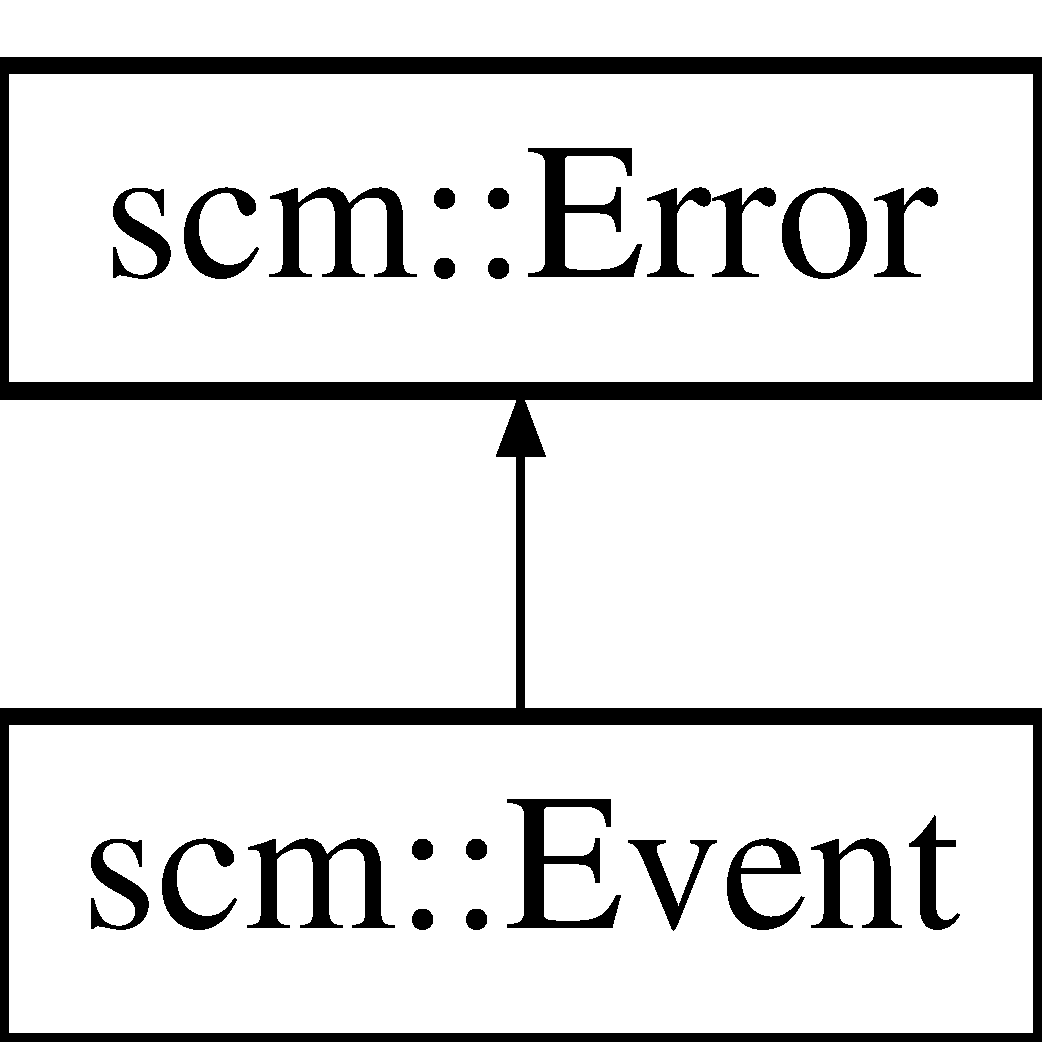
\includegraphics[height=2cm]{classscm_1_1_error}
\end{center}
\end{figure}
\subsection*{Public Member Functions}
\begin{DoxyCompactItemize}
\item 
\hyperlink{classscm_1_1_error_a9c6aa255ce180155a748f304f83830d3}{Error} (\hyperlink{namespacescm_a13a6ecf77ceb7b5b3a38e0fada54aa99}{ErrString} es)
\item 
virtual bool \hyperlink{classscm_1_1_error_a2660b73f9671be3f286bed9d622a926a}{Ok} ()=0
\item 
\hyperlink{namespacescm_a13a6ecf77ceb7b5b3a38e0fada54aa99}{ErrString} \hyperlink{classscm_1_1_error_a8fa002269b2ea7b0af4581951a7908f0}{Err} ()
\item 
void \hyperlink{classscm_1_1_error_aa4309b2556e84bd9bc6c7871f3be2f7a}{Err} (\hyperlink{namespacescm_a13a6ecf77ceb7b5b3a38e0fada54aa99}{ErrString} es)
\item 
void \hyperlink{classscm_1_1_error_a4dc4a630569665a615a0bfb321b65238}{ReportErr} ()
\item 
void \hyperlink{classscm_1_1_error_ace08c93643469a92cb3ca1e0fb1ca583}{SetReportErr} (\hyperlink{namespacescm_a13a6ecf77ceb7b5b3a38e0fada54aa99}{ErrString} es)
\item 
void \hyperlink{classscm_1_1_error_a3d3598611ee2955f3144ec2602b69677}{ClassName} (std::string cn)
\end{DoxyCompactItemize}


\subsection{Detailed Description}


Definition at line 9 of file error.h.



\subsection{Constructor \& Destructor Documentation}
\hypertarget{classscm_1_1_error_a9c6aa255ce180155a748f304f83830d3}{
\index{scm::Error@{scm::Error}!Error@{Error}}
\index{Error@{Error}!scm::Error@{scm::Error}}
\subsubsection[{Error}]{\setlength{\rightskip}{0pt plus 5cm}scm::Error::Error ({\bf ErrString} {\em es})}}
\label{classscm_1_1_error_a9c6aa255ce180155a748f304f83830d3}


Definition at line 11 of file error.cc.



\subsection{Member Function Documentation}
\hypertarget{classscm_1_1_error_a3d3598611ee2955f3144ec2602b69677}{
\index{scm::Error@{scm::Error}!ClassName@{ClassName}}
\index{ClassName@{ClassName}!scm::Error@{scm::Error}}
\subsubsection[{ClassName}]{\setlength{\rightskip}{0pt plus 5cm}void scm::Error::ClassName (std::string {\em cn})\hspace{0.3cm}{\ttfamily  \mbox{[}inline\mbox{]}}}}
\label{classscm_1_1_error_a3d3598611ee2955f3144ec2602b69677}


Definition at line 25 of file error.h.

\hypertarget{classscm_1_1_error_aa4309b2556e84bd9bc6c7871f3be2f7a}{
\index{scm::Error@{scm::Error}!Err@{Err}}
\index{Err@{Err}!scm::Error@{scm::Error}}
\subsubsection[{Err}]{\setlength{\rightskip}{0pt plus 5cm}void scm::Error::Err ({\bf scm::ErrString} {\em es})}}
\label{classscm_1_1_error_aa4309b2556e84bd9bc6c7871f3be2f7a}


Definition at line 21 of file error.cc.

\hypertarget{classscm_1_1_error_a8fa002269b2ea7b0af4581951a7908f0}{
\index{scm::Error@{scm::Error}!Err@{Err}}
\index{Err@{Err}!scm::Error@{scm::Error}}
\subsubsection[{Err}]{\setlength{\rightskip}{0pt plus 5cm}{\bf ErrString} scm::Error::Err ()}}
\label{classscm_1_1_error_a8fa002269b2ea7b0af4581951a7908f0}


Definition at line 15 of file error.cc.

\hypertarget{classscm_1_1_error_a2660b73f9671be3f286bed9d622a926a}{
\index{scm::Error@{scm::Error}!Ok@{Ok}}
\index{Ok@{Ok}!scm::Error@{scm::Error}}
\subsubsection[{Ok}]{\setlength{\rightskip}{0pt plus 5cm}virtual bool scm::Error::Ok ()\hspace{0.3cm}{\ttfamily  \mbox{[}pure virtual\mbox{]}}}}
\label{classscm_1_1_error_a2660b73f9671be3f286bed9d622a926a}


Implemented in \hyperlink{classscm_1_1_event_a95400a0d0218dfb664c028d1130a5d14}{scm::Event}.

\hypertarget{classscm_1_1_error_a4dc4a630569665a615a0bfb321b65238}{
\index{scm::Error@{scm::Error}!ReportErr@{ReportErr}}
\index{ReportErr@{ReportErr}!scm::Error@{scm::Error}}
\subsubsection[{ReportErr}]{\setlength{\rightskip}{0pt plus 5cm}void scm::Error::ReportErr ()}}
\label{classscm_1_1_error_a4dc4a630569665a615a0bfb321b65238}


Definition at line 29 of file error.cc.

\hypertarget{classscm_1_1_error_ace08c93643469a92cb3ca1e0fb1ca583}{
\index{scm::Error@{scm::Error}!SetReportErr@{SetReportErr}}
\index{SetReportErr@{SetReportErr}!scm::Error@{scm::Error}}
\subsubsection[{SetReportErr}]{\setlength{\rightskip}{0pt plus 5cm}void scm::Error::SetReportErr ({\bf ErrString} {\em es})}}
\label{classscm_1_1_error_ace08c93643469a92cb3ca1e0fb1ca583}


Definition at line 33 of file error.cc.



The documentation for this class was generated from the following files:\begin{DoxyCompactItemize}
\item 
/home/derek/dev/crml/crml/src/sys/\hyperlink{error_8h}{error.h}\item 
/home/derek/dev/crml/crml/src/sys/\hyperlink{error_8cc}{error.cc}\end{DoxyCompactItemize}

\hypertarget{classscm_1_1_event}{
\section{scm::Event Class Reference}
\label{classscm_1_1_event}\index{scm::Event@{scm::Event}}
}


{\ttfamily \#include $<$event.h$>$}

Inheritance diagram for scm::Event:\begin{figure}[H]
\begin{center}
\leavevmode
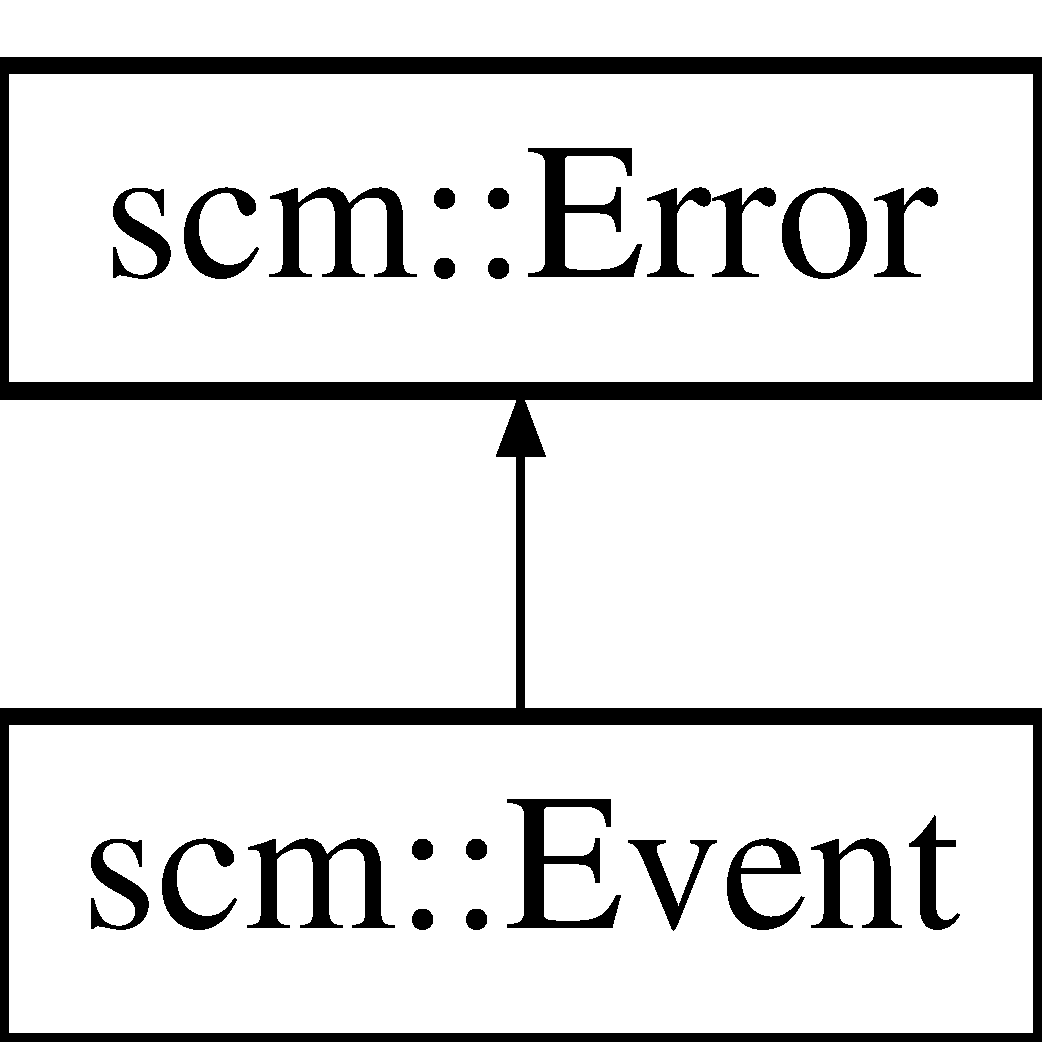
\includegraphics[height=2cm]{classscm_1_1_event}
\end{center}
\end{figure}
\subsection*{Public Member Functions}
\begin{DoxyCompactItemize}
\item 
\hyperlink{classscm_1_1_event_ae0b0fbe856c9fbce52b50e08860946e8}{Event} ()
\item 
\hyperlink{classscm_1_1_event_a4f22bf217daf2b5e3670e987579fb152}{$\sim$Event} ()
\item 
void \hyperlink{classscm_1_1_event_a2dfdf12d5b7918b2102e7ce1c4142ed3}{Init} ()
\item 
void \hyperlink{classscm_1_1_event_a1e1aa9fbe9b5e7e7c9b0ff8f0ba74cd2}{PushEvent} (\hyperlink{struct___n_p_pepper_event}{NPPepperEvent} $\ast$evt)
\item 
bool \hyperlink{classscm_1_1_event_ae736ee83efd335726cad841b6082e491}{Empty} ()
\item 
void \hyperlink{classscm_1_1_event_aba1e9492e1d03bd67afb9c8943e89fe9}{Drain} ()
\item 
\hyperlink{struct___n_p_pepper_event}{NPPepperEvent} $\ast$ \hyperlink{classscm_1_1_event_aaa7905956b3d789fa16cc7a73490dc5e}{PopEvent} ()
\item 
virtual bool \hyperlink{classscm_1_1_event_a95400a0d0218dfb664c028d1130a5d14}{Ok} ()
\end{DoxyCompactItemize}


\subsection{Detailed Description}


Definition at line 19 of file event.h.



\subsection{Constructor \& Destructor Documentation}
\hypertarget{classscm_1_1_event_ae0b0fbe856c9fbce52b50e08860946e8}{
\index{scm::Event@{scm::Event}!Event@{Event}}
\index{Event@{Event}!scm::Event@{scm::Event}}
\subsubsection[{Event}]{\setlength{\rightskip}{0pt plus 5cm}scm::Event::Event ()\hspace{0.3cm}{\ttfamily  \mbox{[}inline, explicit\mbox{]}}}}
\label{classscm_1_1_event_ae0b0fbe856c9fbce52b50e08860946e8}


Definition at line 21 of file event.h.

\hypertarget{classscm_1_1_event_a4f22bf217daf2b5e3670e987579fb152}{
\index{scm::Event@{scm::Event}!$\sim$Event@{$\sim$Event}}
\index{$\sim$Event@{$\sim$Event}!scm::Event@{scm::Event}}
\subsubsection[{$\sim$Event}]{\setlength{\rightskip}{0pt plus 5cm}scm::Event::$\sim$Event ()}}
\label{classscm_1_1_event_a4f22bf217daf2b5e3670e987579fb152}


Definition at line 17 of file event.cc.



\subsection{Member Function Documentation}
\hypertarget{classscm_1_1_event_aba1e9492e1d03bd67afb9c8943e89fe9}{
\index{scm::Event@{scm::Event}!Drain@{Drain}}
\index{Drain@{Drain}!scm::Event@{scm::Event}}
\subsubsection[{Drain}]{\setlength{\rightskip}{0pt plus 5cm}void scm::Event::Drain ()}}
\label{classscm_1_1_event_aba1e9492e1d03bd67afb9c8943e89fe9}


Definition at line 59 of file event.cc.

\hypertarget{classscm_1_1_event_ae736ee83efd335726cad841b6082e491}{
\index{scm::Event@{scm::Event}!Empty@{Empty}}
\index{Empty@{Empty}!scm::Event@{scm::Event}}
\subsubsection[{Empty}]{\setlength{\rightskip}{0pt plus 5cm}bool scm::Event::Empty ()}}
\label{classscm_1_1_event_ae736ee83efd335726cad841b6082e491}


Definition at line 26 of file event.cc.

\hypertarget{classscm_1_1_event_a2dfdf12d5b7918b2102e7ce1c4142ed3}{
\index{scm::Event@{scm::Event}!Init@{Init}}
\index{Init@{Init}!scm::Event@{scm::Event}}
\subsubsection[{Init}]{\setlength{\rightskip}{0pt plus 5cm}void scm::Event::Init ()}}
\label{classscm_1_1_event_a2dfdf12d5b7918b2102e7ce1c4142ed3}


Definition at line 21 of file event.cc.

\hypertarget{classscm_1_1_event_a95400a0d0218dfb664c028d1130a5d14}{
\index{scm::Event@{scm::Event}!Ok@{Ok}}
\index{Ok@{Ok}!scm::Event@{scm::Event}}
\subsubsection[{Ok}]{\setlength{\rightskip}{0pt plus 5cm}bool scm::Event::Ok ()\hspace{0.3cm}{\ttfamily  \mbox{[}virtual\mbox{]}}}}
\label{classscm_1_1_event_a95400a0d0218dfb664c028d1130a5d14}


Implements \hyperlink{classscm_1_1_error_a2660b73f9671be3f286bed9d622a926a}{scm::Error}.



Definition at line 13 of file event.cc.

\hypertarget{classscm_1_1_event_aaa7905956b3d789fa16cc7a73490dc5e}{
\index{scm::Event@{scm::Event}!PopEvent@{PopEvent}}
\index{PopEvent@{PopEvent}!scm::Event@{scm::Event}}
\subsubsection[{PopEvent}]{\setlength{\rightskip}{0pt plus 5cm}{\bf NPPepperEvent} $\ast$ scm::Event::PopEvent ()}}
\label{classscm_1_1_event_aaa7905956b3d789fa16cc7a73490dc5e}


Definition at line 50 of file event.cc.

\hypertarget{classscm_1_1_event_a1e1aa9fbe9b5e7e7c9b0ff8f0ba74cd2}{
\index{scm::Event@{scm::Event}!PushEvent@{PushEvent}}
\index{PushEvent@{PushEvent}!scm::Event@{scm::Event}}
\subsubsection[{PushEvent}]{\setlength{\rightskip}{0pt plus 5cm}void scm::Event::PushEvent ({\bf NPPepperEvent} $\ast$ {\em evt})}}
\label{classscm_1_1_event_a1e1aa9fbe9b5e7e7c9b0ff8f0ba74cd2}


Definition at line 65 of file event.cc.



The documentation for this class was generated from the following files:\begin{DoxyCompactItemize}
\item 
/home/derek/dev/cell-\/grid-\/game/nacl/crml/crml/evt/\hyperlink{event_8h}{event.h}\item 
/home/derek/dev/cell-\/grid-\/game/nacl/crml/crml/evt/\hyperlink{event_8cc}{event.cc}\end{DoxyCompactItemize}

\hypertarget{class_event_handler}{
\section{EventHandler Class Reference}
\label{class_event_handler}\index{EventHandler@{EventHandler}}
}


{\ttfamily \#include $<$event\_\-handler.h$>$}

\subsection*{Public Member Functions}
\begin{DoxyCompactItemize}
\item 
\hyperlink{class_event_handler_a6b7f9af8b5c3c4128047d35467ca0da0}{EventHandler} (\hyperlink{struct___n_p_p}{NPP} npp)
\item 
\hyperlink{class_event_handler_a3decb8cd88ba8af2b9b0b0f0f2fcd722}{$\sim$EventHandler} ()
\item 
bool \hyperlink{class_event_handler_a18771c6be120edf9d912a4003066b8b3}{addText} (const char $\ast$cstr)
\item 
int \hyperlink{class_event_handler_a2fcafd6f528017d8a814f9c384e2e057}{handle} (void $\ast$event)
\item 
bool \hyperlink{class_event_handler_a2f334e3eb39be72751e342619489e695}{is\_\-text\_\-box\_\-set} ()
\item 
bool \hyperlink{class_event_handler_aa09c0b995aa6c774d4a33be13be0cbf2}{set\_\-text\_\-box} (NPObject $\ast$text\_\-box\_\-object)
\item 
void \hyperlink{class_event_handler_a67d149352861c0a8fe603a14585d1003}{Init} (\hyperlink{classscm_1_1_event}{scm::Event} $\ast$)
\end{DoxyCompactItemize}


\subsection{Detailed Description}


Definition at line 34 of file event\_\-handler.h.



\subsection{Constructor \& Destructor Documentation}
\hypertarget{class_event_handler_a6b7f9af8b5c3c4128047d35467ca0da0}{
\index{EventHandler@{EventHandler}!EventHandler@{EventHandler}}
\index{EventHandler@{EventHandler}!EventHandler@{EventHandler}}
\subsubsection[{EventHandler}]{\setlength{\rightskip}{0pt plus 5cm}EventHandler::EventHandler ({\bf NPP} {\em npp})\hspace{0.3cm}{\ttfamily  \mbox{[}explicit\mbox{]}}}}
\label{class_event_handler_a6b7f9af8b5c3c4128047d35467ca0da0}


Definition at line 57 of file event\_\-handler.cc.

\hypertarget{class_event_handler_a3decb8cd88ba8af2b9b0b0f0f2fcd722}{
\index{EventHandler@{EventHandler}!$\sim$EventHandler@{$\sim$EventHandler}}
\index{$\sim$EventHandler@{$\sim$EventHandler}!EventHandler@{EventHandler}}
\subsubsection[{$\sim$EventHandler}]{\setlength{\rightskip}{0pt plus 5cm}EventHandler::$\sim$EventHandler ()}}
\label{class_event_handler_a3decb8cd88ba8af2b9b0b0f0f2fcd722}


Definition at line 62 of file event\_\-handler.cc.



\subsection{Member Function Documentation}
\hypertarget{class_event_handler_a18771c6be120edf9d912a4003066b8b3}{
\index{EventHandler@{EventHandler}!addText@{addText}}
\index{addText@{addText}!EventHandler@{EventHandler}}
\subsubsection[{addText}]{\setlength{\rightskip}{0pt plus 5cm}bool EventHandler::addText (const char $\ast$ {\em cstr})}}
\label{class_event_handler_a18771c6be120edf9d912a4003066b8b3}


Definition at line 71 of file event\_\-handler.cc.

\hypertarget{class_event_handler_a2fcafd6f528017d8a814f9c384e2e057}{
\index{EventHandler@{EventHandler}!handle@{handle}}
\index{handle@{handle}!EventHandler@{EventHandler}}
\subsubsection[{handle}]{\setlength{\rightskip}{0pt plus 5cm}int EventHandler::handle (void $\ast$ {\em event})}}
\label{class_event_handler_a2fcafd6f528017d8a814f9c384e2e057}


Definition at line 121 of file event\_\-handler.cc.

\hypertarget{class_event_handler_a67d149352861c0a8fe603a14585d1003}{
\index{EventHandler@{EventHandler}!Init@{Init}}
\index{Init@{Init}!EventHandler@{EventHandler}}
\subsubsection[{Init}]{\setlength{\rightskip}{0pt plus 5cm}void EventHandler::Init ({\bf scm::Event} $\ast$ {\em sys})}}
\label{class_event_handler_a67d149352861c0a8fe603a14585d1003}


Definition at line 65 of file event\_\-handler.cc.

\hypertarget{class_event_handler_a2f334e3eb39be72751e342619489e695}{
\index{EventHandler@{EventHandler}!is\_\-text\_\-box\_\-set@{is\_\-text\_\-box\_\-set}}
\index{is\_\-text\_\-box\_\-set@{is\_\-text\_\-box\_\-set}!EventHandler@{EventHandler}}
\subsubsection[{is\_\-text\_\-box\_\-set}]{\setlength{\rightskip}{0pt plus 5cm}bool EventHandler::is\_\-text\_\-box\_\-set ()}}
\label{class_event_handler_a2f334e3eb39be72751e342619489e695}


Definition at line 187 of file event\_\-handler.cc.

\hypertarget{class_event_handler_aa09c0b995aa6c774d4a33be13be0cbf2}{
\index{EventHandler@{EventHandler}!set\_\-text\_\-box@{set\_\-text\_\-box}}
\index{set\_\-text\_\-box@{set\_\-text\_\-box}!EventHandler@{EventHandler}}
\subsubsection[{set\_\-text\_\-box}]{\setlength{\rightskip}{0pt plus 5cm}bool EventHandler::set\_\-text\_\-box (NPObject $\ast$ {\em text\_\-box\_\-object})}}
\label{class_event_handler_aa09c0b995aa6c774d4a33be13be0cbf2}


Definition at line 193 of file event\_\-handler.cc.



The documentation for this class was generated from the following files:\begin{DoxyCompactItemize}
\item 
/home/derek/dev/cell-\/grid-\/game/nacl/crml/crml/evt/\hyperlink{event__handler_8h}{event\_\-handler.h}\item 
/home/derek/dev/cell-\/grid-\/game/nacl/crml/crml/evt/\hyperlink{event__handler_8cc}{event\_\-handler.cc}\end{DoxyCompactItemize}

\hypertarget{struct_hello_world}{
\section{HelloWorld Struct Reference}
\label{struct_hello_world}\index{HelloWorld@{HelloWorld}}
}
\subsection*{Public Attributes}
\begin{DoxyCompactItemize}
\item 
\hyperlink{struct___n_p_p}{NPP} \hyperlink{struct_hello_world_a8546fa606713a22cd373527986469eba}{npp}
\item 
\hyperlink{struct_n_p_object}{NPObject} $\ast$ \hyperlink{struct_hello_world_ab53916603277423408f4e4997b3b5733}{npobject}
\end{DoxyCompactItemize}


\subsection{Detailed Description}


Definition at line 13 of file npp\_\-gate.cc.



\subsection{Member Data Documentation}
\hypertarget{struct_hello_world_ab53916603277423408f4e4997b3b5733}{
\index{HelloWorld@{HelloWorld}!npobject@{npobject}}
\index{npobject@{npobject}!HelloWorld@{HelloWorld}}
\subsubsection[{npobject}]{\setlength{\rightskip}{0pt plus 5cm}{\bf NPObject}$\ast$ {\bf HelloWorld::npobject}}}
\label{struct_hello_world_ab53916603277423408f4e4997b3b5733}


Definition at line 15 of file npp\_\-gate.cc.

\hypertarget{struct_hello_world_a8546fa606713a22cd373527986469eba}{
\index{HelloWorld@{HelloWorld}!npp@{npp}}
\index{npp@{npp}!HelloWorld@{HelloWorld}}
\subsubsection[{npp}]{\setlength{\rightskip}{0pt plus 5cm}{\bf NPP} {\bf HelloWorld::npp}}}
\label{struct_hello_world_a8546fa606713a22cd373527986469eba}


Definition at line 14 of file npp\_\-gate.cc.



The documentation for this struct was generated from the following file:\begin{DoxyCompactItemize}
\item 
/home/derek/dev/cell-\/grid-\/game/nacl/crml/crml/sys/\hyperlink{sys_2npp__gate_8cc}{npp\_\-gate.cc}\end{DoxyCompactItemize}

\hypertarget{class_hello_world_instance}{
\section{HelloWorldInstance Class Reference}
\label{class_hello_world_instance}\index{HelloWorldInstance@{HelloWorldInstance}}
}
\subsection*{Public Member Functions}
\begin{DoxyCompactItemize}
\item 
\hyperlink{class_hello_world_instance_add03eac81a09900135582a464bfcd8f8}{HelloWorldInstance} (PP\_\-Instance instance)
\item 
virtual \hyperlink{class_hello_world_instance_ab82a0f1aa35b3f8fbc2e107af026bfc5}{$\sim$HelloWorldInstance} ()
\item 
virtual pp::Var \hyperlink{class_hello_world_instance_ac489a6775aead72dc1b17d22d1eb6688}{GetInstanceObject} ()
\end{DoxyCompactItemize}


\subsection{Detailed Description}


Definition at line 102 of file hello\_\-world.cc.



\subsection{Constructor \& Destructor Documentation}
\hypertarget{class_hello_world_instance_add03eac81a09900135582a464bfcd8f8}{
\index{HelloWorldInstance@{HelloWorldInstance}!HelloWorldInstance@{HelloWorldInstance}}
\index{HelloWorldInstance@{HelloWorldInstance}!HelloWorldInstance@{HelloWorldInstance}}
\subsubsection[{HelloWorldInstance}]{\setlength{\rightskip}{0pt plus 5cm}HelloWorldInstance::HelloWorldInstance (PP\_\-Instance {\em instance})\hspace{0.3cm}{\ttfamily  \mbox{[}inline\mbox{]}}}}
\label{class_hello_world_instance_add03eac81a09900135582a464bfcd8f8}


Definition at line 104 of file hello\_\-world.cc.

\hypertarget{class_hello_world_instance_ab82a0f1aa35b3f8fbc2e107af026bfc5}{
\index{HelloWorldInstance@{HelloWorldInstance}!$\sim$HelloWorldInstance@{$\sim$HelloWorldInstance}}
\index{$\sim$HelloWorldInstance@{$\sim$HelloWorldInstance}!HelloWorldInstance@{HelloWorldInstance}}
\subsubsection[{$\sim$HelloWorldInstance}]{\setlength{\rightskip}{0pt plus 5cm}virtual HelloWorldInstance::$\sim$HelloWorldInstance ()\hspace{0.3cm}{\ttfamily  \mbox{[}inline, virtual\mbox{]}}}}
\label{class_hello_world_instance_ab82a0f1aa35b3f8fbc2e107af026bfc5}


Definition at line 105 of file hello\_\-world.cc.



\subsection{Member Function Documentation}
\hypertarget{class_hello_world_instance_ac489a6775aead72dc1b17d22d1eb6688}{
\index{HelloWorldInstance@{HelloWorldInstance}!GetInstanceObject@{GetInstanceObject}}
\index{GetInstanceObject@{GetInstanceObject}!HelloWorldInstance@{HelloWorldInstance}}
\subsubsection[{GetInstanceObject}]{\setlength{\rightskip}{0pt plus 5cm}virtual pp::Var HelloWorldInstance::GetInstanceObject ()\hspace{0.3cm}{\ttfamily  \mbox{[}inline, virtual\mbox{]}}}}
\label{class_hello_world_instance_ac489a6775aead72dc1b17d22d1eb6688}


Definition at line 108 of file hello\_\-world.cc.



The documentation for this class was generated from the following file:\begin{DoxyCompactItemize}
\item 
/home/derek/dev/crml/crml/test/hello\_\-world/\hyperlink{hello__world_8cc}{hello\_\-world.cc}\end{DoxyCompactItemize}

\hypertarget{class_hello_world_module}{
\section{HelloWorldModule Class Reference}
\label{class_hello_world_module}\index{HelloWorldModule@{HelloWorldModule}}
}
\subsection*{Public Member Functions}
\begin{DoxyCompactItemize}
\item 
\hyperlink{class_hello_world_module_a51bebf2cbff1d8914b988101781bd01d}{HelloWorldModule} ()
\item 
virtual \hyperlink{class_hello_world_module_a2458f9ee6a26568e54c6bd3a0323abcf}{$\sim$HelloWorldModule} ()
\item 
virtual pp::Instance $\ast$ \hyperlink{class_hello_world_module_a6ee0eeeb3ed2f95b819adfd4df33c47f}{CreateInstance} (PP\_\-Instance instance)
\end{DoxyCompactItemize}


\subsection{Detailed Description}


Definition at line 117 of file hello\_\-world.cc.



\subsection{Constructor \& Destructor Documentation}
\hypertarget{class_hello_world_module_a51bebf2cbff1d8914b988101781bd01d}{
\index{HelloWorldModule@{HelloWorldModule}!HelloWorldModule@{HelloWorldModule}}
\index{HelloWorldModule@{HelloWorldModule}!HelloWorldModule@{HelloWorldModule}}
\subsubsection[{HelloWorldModule}]{\setlength{\rightskip}{0pt plus 5cm}HelloWorldModule::HelloWorldModule ()\hspace{0.3cm}{\ttfamily  \mbox{[}inline\mbox{]}}}}
\label{class_hello_world_module_a51bebf2cbff1d8914b988101781bd01d}


Definition at line 119 of file hello\_\-world.cc.

\hypertarget{class_hello_world_module_a2458f9ee6a26568e54c6bd3a0323abcf}{
\index{HelloWorldModule@{HelloWorldModule}!$\sim$HelloWorldModule@{$\sim$HelloWorldModule}}
\index{$\sim$HelloWorldModule@{$\sim$HelloWorldModule}!HelloWorldModule@{HelloWorldModule}}
\subsubsection[{$\sim$HelloWorldModule}]{\setlength{\rightskip}{0pt plus 5cm}virtual HelloWorldModule::$\sim$HelloWorldModule ()\hspace{0.3cm}{\ttfamily  \mbox{[}inline, virtual\mbox{]}}}}
\label{class_hello_world_module_a2458f9ee6a26568e54c6bd3a0323abcf}


Definition at line 120 of file hello\_\-world.cc.



\subsection{Member Function Documentation}
\hypertarget{class_hello_world_module_a6ee0eeeb3ed2f95b819adfd4df33c47f}{
\index{HelloWorldModule@{HelloWorldModule}!CreateInstance@{CreateInstance}}
\index{CreateInstance@{CreateInstance}!HelloWorldModule@{HelloWorldModule}}
\subsubsection[{CreateInstance}]{\setlength{\rightskip}{0pt plus 5cm}virtual pp::Instance$\ast$ HelloWorldModule::CreateInstance (PP\_\-Instance {\em instance})\hspace{0.3cm}{\ttfamily  \mbox{[}inline, virtual\mbox{]}}}}
\label{class_hello_world_module_a6ee0eeeb3ed2f95b819adfd4df33c47f}


Definition at line 123 of file hello\_\-world.cc.



The documentation for this class was generated from the following file:\begin{DoxyCompactItemize}
\item 
/home/derek/dev/cell-\/grid-\/game/nacl/crml/crml/test/hello\_\-world/\hyperlink{hello__world_8cc}{hello\_\-world.cc}\end{DoxyCompactItemize}

\hypertarget{class_hello_world_scriptable_object}{
\section{HelloWorldScriptableObject Class Reference}
\label{class_hello_world_scriptable_object}\index{HelloWorldScriptableObject@{HelloWorldScriptableObject}}
}
\subsection*{Public Member Functions}
\begin{DoxyCompactItemize}
\item 
virtual bool \hyperlink{class_hello_world_scriptable_object_a0af23165c74483e47f97877cbb51e79a}{HasMethod} (const pp::Var \&method, pp::Var $\ast$exception)
\item 
virtual pp::Var \hyperlink{class_hello_world_scriptable_object_a217b4b958a4bfb250dd8ac588ab794ad}{Call} (const pp::Var \&method, const std::vector$<$ pp::Var $>$ \&args, pp::Var $\ast$exception)
\end{DoxyCompactItemize}


\subsection{Detailed Description}


Definition at line 53 of file hello\_\-world.cc.



\subsection{Member Function Documentation}
\hypertarget{class_hello_world_scriptable_object_a217b4b958a4bfb250dd8ac588ab794ad}{
\index{HelloWorldScriptableObject@{HelloWorldScriptableObject}!Call@{Call}}
\index{Call@{Call}!HelloWorldScriptableObject@{HelloWorldScriptableObject}}
\subsubsection[{Call}]{\setlength{\rightskip}{0pt plus 5cm}pp::Var HelloWorldScriptableObject::Call (const pp::Var \& {\em method}, \/  const std::vector$<$ pp::Var $>$ \& {\em args}, \/  pp::Var $\ast$ {\em exception})\hspace{0.3cm}{\ttfamily  \mbox{[}virtual\mbox{]}}}}
\label{class_hello_world_scriptable_object_a217b4b958a4bfb250dd8ac588ab794ad}


Definition at line 77 of file hello\_\-world.cc.

\hypertarget{class_hello_world_scriptable_object_a0af23165c74483e47f97877cbb51e79a}{
\index{HelloWorldScriptableObject@{HelloWorldScriptableObject}!HasMethod@{HasMethod}}
\index{HasMethod@{HasMethod}!HelloWorldScriptableObject@{HelloWorldScriptableObject}}
\subsubsection[{HasMethod}]{\setlength{\rightskip}{0pt plus 5cm}bool HelloWorldScriptableObject::HasMethod (const pp::Var \& {\em method}, \/  pp::Var $\ast$ {\em exception})\hspace{0.3cm}{\ttfamily  \mbox{[}virtual\mbox{]}}}}
\label{class_hello_world_scriptable_object_a0af23165c74483e47f97877cbb51e79a}


Definition at line 66 of file hello\_\-world.cc.



The documentation for this class was generated from the following file:\begin{DoxyCompactItemize}
\item 
/home/derek/dev/cell-\/grid-\/game/nacl/crml/crml/test/hello\_\-world/\hyperlink{hello__world_8cc}{hello\_\-world.cc}\end{DoxyCompactItemize}

\hypertarget{classscm_1_1_hex_store}{
\section{scm::HexStore Class Reference}
\label{classscm_1_1_hex_store}\index{scm::HexStore@{scm::HexStore}}
}


{\ttfamily \#include $<$hex\_\-store.h$>$}

\subsection*{Public Member Functions}
\begin{DoxyCompactItemize}
\item 
\hyperlink{classscm_1_1_hex_store_ae3ea77bf45ef55916e02aba5f5d280f5}{HexStore} ()
\item 
\hyperlink{classscm_1_1_hex_store_ac418965e7e9ee7569bb03b7230bad1bd}{$\sim$HexStore} ()
\item 
bool \hyperlink{classscm_1_1_hex_store_ae8d894818fe0859462b63f2e34d08a33}{Ok} ()
\item 
int \hyperlink{classscm_1_1_hex_store_a85cbfdc7f9a41355db174d3b96382d79}{Err} ()
\item 
void \hyperlink{classscm_1_1_hex_store_ac98d4c0f37c642e6b45262ec1db62d80}{ReportErr} ()
\item 
void \hyperlink{classscm_1_1_hex_store_aa1792118dbb32383976d6906c69c9e71}{Store} (std::string, std::string)
\item 
int \hyperlink{classscm_1_1_hex_store_a277a7c2220511ad3c0e447802589def1}{ValLength} (std::string)
\item 
bool \hyperlink{classscm_1_1_hex_store_a2c7a1fc73741e0b3613516388b562475}{EmptyVal} (std::string)
\item 
void \hyperlink{classscm_1_1_hex_store_ac086449d331c2e0dd6eaf11a003ffe99}{Append} (std::string, std::string)
\item 
std::string \hyperlink{classscm_1_1_hex_store_acdc20757093a52e3f7748dea41d185b2}{GetValue} (std::string)
\item 
const char $\ast$ \hyperlink{classscm_1_1_hex_store_a5e12c88428e17be9bb8f6c08ab107e57}{ByteArray} (std::string)
\end{DoxyCompactItemize}


\subsection{Detailed Description}


Definition at line 19 of file hex\_\-store.h.



\subsection{Constructor \& Destructor Documentation}
\hypertarget{classscm_1_1_hex_store_ae3ea77bf45ef55916e02aba5f5d280f5}{
\index{scm::HexStore@{scm::HexStore}!HexStore@{HexStore}}
\index{HexStore@{HexStore}!scm::HexStore@{scm::HexStore}}
\subsubsection[{HexStore}]{\setlength{\rightskip}{0pt plus 5cm}scm::HexStore::HexStore ()}}
\label{classscm_1_1_hex_store_ae3ea77bf45ef55916e02aba5f5d280f5}


Definition at line 11 of file hex\_\-store.cc.

\hypertarget{classscm_1_1_hex_store_ac418965e7e9ee7569bb03b7230bad1bd}{
\index{scm::HexStore@{scm::HexStore}!$\sim$HexStore@{$\sim$HexStore}}
\index{$\sim$HexStore@{$\sim$HexStore}!scm::HexStore@{scm::HexStore}}
\subsubsection[{$\sim$HexStore}]{\setlength{\rightskip}{0pt plus 5cm}scm::HexStore::$\sim$HexStore ()}}
\label{classscm_1_1_hex_store_ac418965e7e9ee7569bb03b7230bad1bd}


Definition at line 12 of file hex\_\-store.cc.



\subsection{Member Function Documentation}
\hypertarget{classscm_1_1_hex_store_ac086449d331c2e0dd6eaf11a003ffe99}{
\index{scm::HexStore@{scm::HexStore}!Append@{Append}}
\index{Append@{Append}!scm::HexStore@{scm::HexStore}}
\subsubsection[{Append}]{\setlength{\rightskip}{0pt plus 5cm}void scm::HexStore::Append (std::string {\em key}, \/  std::string {\em val})}}
\label{classscm_1_1_hex_store_ac086449d331c2e0dd6eaf11a003ffe99}


Definition at line 67 of file hex\_\-store.cc.

\hypertarget{classscm_1_1_hex_store_a5e12c88428e17be9bb8f6c08ab107e57}{
\index{scm::HexStore@{scm::HexStore}!ByteArray@{ByteArray}}
\index{ByteArray@{ByteArray}!scm::HexStore@{scm::HexStore}}
\subsubsection[{ByteArray}]{\setlength{\rightskip}{0pt plus 5cm}const char $\ast$ scm::HexStore::ByteArray (std::string {\em key})}}
\label{classscm_1_1_hex_store_a5e12c88428e17be9bb8f6c08ab107e57}


Definition at line 79 of file hex\_\-store.cc.

\hypertarget{classscm_1_1_hex_store_a2c7a1fc73741e0b3613516388b562475}{
\index{scm::HexStore@{scm::HexStore}!EmptyVal@{EmptyVal}}
\index{EmptyVal@{EmptyVal}!scm::HexStore@{scm::HexStore}}
\subsubsection[{EmptyVal}]{\setlength{\rightskip}{0pt plus 5cm}bool scm::HexStore::EmptyVal (std::string {\em key})}}
\label{classscm_1_1_hex_store_a2c7a1fc73741e0b3613516388b562475}


Definition at line 45 of file hex\_\-store.cc.

\hypertarget{classscm_1_1_hex_store_a85cbfdc7f9a41355db174d3b96382d79}{
\index{scm::HexStore@{scm::HexStore}!Err@{Err}}
\index{Err@{Err}!scm::HexStore@{scm::HexStore}}
\subsubsection[{Err}]{\setlength{\rightskip}{0pt plus 5cm}int scm::HexStore::Err ()}}
\label{classscm_1_1_hex_store_a85cbfdc7f9a41355db174d3b96382d79}


Definition at line 15 of file hex\_\-store.cc.

\hypertarget{classscm_1_1_hex_store_acdc20757093a52e3f7748dea41d185b2}{
\index{scm::HexStore@{scm::HexStore}!GetValue@{GetValue}}
\index{GetValue@{GetValue}!scm::HexStore@{scm::HexStore}}
\subsubsection[{GetValue}]{\setlength{\rightskip}{0pt plus 5cm}std::string scm::HexStore::GetValue (std::string {\em key})}}
\label{classscm_1_1_hex_store_acdc20757093a52e3f7748dea41d185b2}


Definition at line 58 of file hex\_\-store.cc.

\hypertarget{classscm_1_1_hex_store_ae8d894818fe0859462b63f2e34d08a33}{
\index{scm::HexStore@{scm::HexStore}!Ok@{Ok}}
\index{Ok@{Ok}!scm::HexStore@{scm::HexStore}}
\subsubsection[{Ok}]{\setlength{\rightskip}{0pt plus 5cm}bool scm::HexStore::Ok ()}}
\label{classscm_1_1_hex_store_ae8d894818fe0859462b63f2e34d08a33}


Definition at line 19 of file hex\_\-store.cc.

\hypertarget{classscm_1_1_hex_store_ac98d4c0f37c642e6b45262ec1db62d80}{
\index{scm::HexStore@{scm::HexStore}!ReportErr@{ReportErr}}
\index{ReportErr@{ReportErr}!scm::HexStore@{scm::HexStore}}
\subsubsection[{ReportErr}]{\setlength{\rightskip}{0pt plus 5cm}void scm::HexStore::ReportErr ()}}
\label{classscm_1_1_hex_store_ac98d4c0f37c642e6b45262ec1db62d80}


Definition at line 23 of file hex\_\-store.cc.

\hypertarget{classscm_1_1_hex_store_aa1792118dbb32383976d6906c69c9e71}{
\index{scm::HexStore@{scm::HexStore}!Store@{Store}}
\index{Store@{Store}!scm::HexStore@{scm::HexStore}}
\subsubsection[{Store}]{\setlength{\rightskip}{0pt plus 5cm}void scm::HexStore::Store (std::string {\em key}, \/  std::string {\em val})}}
\label{classscm_1_1_hex_store_aa1792118dbb32383976d6906c69c9e71}


Definition at line 40 of file hex\_\-store.cc.

\hypertarget{classscm_1_1_hex_store_a277a7c2220511ad3c0e447802589def1}{
\index{scm::HexStore@{scm::HexStore}!ValLength@{ValLength}}
\index{ValLength@{ValLength}!scm::HexStore@{scm::HexStore}}
\subsubsection[{ValLength}]{\setlength{\rightskip}{0pt plus 5cm}int scm::HexStore::ValLength (std::string {\em key})}}
\label{classscm_1_1_hex_store_a277a7c2220511ad3c0e447802589def1}


Definition at line 49 of file hex\_\-store.cc.



The documentation for this class was generated from the following files:\begin{DoxyCompactItemize}
\item 
/home/derek/dev/cell-\/grid-\/game/nacl/crml/crml/sys/\hyperlink{hex__store_8h}{hex\_\-store.h}\item 
/home/derek/dev/cell-\/grid-\/game/nacl/crml/crml/sys/\hyperlink{hex__store_8cc}{hex\_\-store.cc}\end{DoxyCompactItemize}

\hypertarget{classscm_1_1_mainloop}{
\section{scm::Mainloop Class Reference}
\label{classscm_1_1_mainloop}\index{scm::Mainloop@{scm::Mainloop}}
}


{\ttfamily \#include $<$loop.h$>$}

\subsection*{Public Member Functions}
\begin{DoxyCompactItemize}
\item 
\hyperlink{classscm_1_1_mainloop_abacbb3c174abded439ddf745e840dd29}{Mainloop} ()
\item 
\hyperlink{classscm_1_1_mainloop_a0638591ae4a2df7e99d2ba586ad5edfe}{$\sim$Mainloop} ()
\item 
void \hyperlink{classscm_1_1_mainloop_a7e332605f463847553999278a975d650}{Go} ()
\item 
\hyperlink{namespacescm_aec9fbdb87d677e6e822d612ed3e3a20b}{MainloopErr} \hyperlink{classscm_1_1_mainloop_a47a4747a4529b29b2337942496bc4e61}{SetFramesPerSecond} (double)
\item 
\hyperlink{namespacescm_aec9fbdb87d677e6e822d612ed3e3a20b}{MainloopErr} \hyperlink{classscm_1_1_mainloop_a3b4177ac538fb42bc7bed6bb5e84a6dc}{Init} (\hyperlink{class_plugin_object}{PluginObject} $\ast$)
\item 
\hyperlink{namespacescm_aec9fbdb87d677e6e822d612ed3e3a20b}{MainloopErr} \hyperlink{classscm_1_1_mainloop_ab4e2e2a9df321c2761d24690a503cc06}{Init2D} (NPDevice $\ast$)
\end{DoxyCompactItemize}


\subsection{Detailed Description}


Definition at line 19 of file loop.h.



\subsection{Constructor \& Destructor Documentation}
\hypertarget{classscm_1_1_mainloop_abacbb3c174abded439ddf745e840dd29}{
\index{scm::Mainloop@{scm::Mainloop}!Mainloop@{Mainloop}}
\index{Mainloop@{Mainloop}!scm::Mainloop@{scm::Mainloop}}
\subsubsection[{Mainloop}]{\setlength{\rightskip}{0pt plus 5cm}scm::Mainloop::Mainloop ()}}
\label{classscm_1_1_mainloop_abacbb3c174abded439ddf745e840dd29}


Definition at line 6 of file loop.cc.

\hypertarget{classscm_1_1_mainloop_a0638591ae4a2df7e99d2ba586ad5edfe}{
\index{scm::Mainloop@{scm::Mainloop}!$\sim$Mainloop@{$\sim$Mainloop}}
\index{$\sim$Mainloop@{$\sim$Mainloop}!scm::Mainloop@{scm::Mainloop}}
\subsubsection[{$\sim$Mainloop}]{\setlength{\rightskip}{0pt plus 5cm}scm::Mainloop::$\sim$Mainloop ()}}
\label{classscm_1_1_mainloop_a0638591ae4a2df7e99d2ba586ad5edfe}


Definition at line 12 of file loop.cc.



\subsection{Member Function Documentation}
\hypertarget{classscm_1_1_mainloop_a7e332605f463847553999278a975d650}{
\index{scm::Mainloop@{scm::Mainloop}!Go@{Go}}
\index{Go@{Go}!scm::Mainloop@{scm::Mainloop}}
\subsubsection[{Go}]{\setlength{\rightskip}{0pt plus 5cm}void scm::Mainloop::Go ()}}
\label{classscm_1_1_mainloop_a7e332605f463847553999278a975d650}


Definition at line 23 of file loop.cc.

\hypertarget{classscm_1_1_mainloop_a3b4177ac538fb42bc7bed6bb5e84a6dc}{
\index{scm::Mainloop@{scm::Mainloop}!Init@{Init}}
\index{Init@{Init}!scm::Mainloop@{scm::Mainloop}}
\subsubsection[{Init}]{\setlength{\rightskip}{0pt plus 5cm}{\bf MainloopErr} scm::Mainloop::Init ({\bf PluginObject} $\ast$ {\em po})}}
\label{classscm_1_1_mainloop_a3b4177ac538fb42bc7bed6bb5e84a6dc}


Definition at line 53 of file loop.cc.

\hypertarget{classscm_1_1_mainloop_ab4e2e2a9df321c2761d24690a503cc06}{
\index{scm::Mainloop@{scm::Mainloop}!Init2D@{Init2D}}
\index{Init2D@{Init2D}!scm::Mainloop@{scm::Mainloop}}
\subsubsection[{Init2D}]{\setlength{\rightskip}{0pt plus 5cm}{\bf MainloopErr} scm::Mainloop::Init2D (NPDevice $\ast$ {\em device2d})}}
\label{classscm_1_1_mainloop_ab4e2e2a9df321c2761d24690a503cc06}


Definition at line 39 of file loop.cc.

\hypertarget{classscm_1_1_mainloop_a47a4747a4529b29b2337942496bc4e61}{
\index{scm::Mainloop@{scm::Mainloop}!SetFramesPerSecond@{SetFramesPerSecond}}
\index{SetFramesPerSecond@{SetFramesPerSecond}!scm::Mainloop@{scm::Mainloop}}
\subsubsection[{SetFramesPerSecond}]{\setlength{\rightskip}{0pt plus 5cm}{\bf MainloopErr} scm::Mainloop::SetFramesPerSecond (double {\em fps})}}
\label{classscm_1_1_mainloop_a47a4747a4529b29b2337942496bc4e61}


Definition at line 47 of file loop.cc.



The documentation for this class was generated from the following files:\begin{DoxyCompactItemize}
\item 
/home/derek/dev/cell-\/grid-\/game/nacl/crml/crml/sys/\hyperlink{loop_8h}{loop.h}\item 
/home/derek/dev/cell-\/grid-\/game/nacl/crml/crml/sys/\hyperlink{loop_8cc}{loop.cc}\end{DoxyCompactItemize}

\hypertarget{struct_m_d5_digest__struct}{
\section{MD5Digest\_\-struct Struct Reference}
\label{struct_m_d5_digest__struct}\index{MD5Digest\_\-struct@{MD5Digest\_\-struct}}
}


{\ttfamily \#include $<$md5.h$>$}

\subsection*{Public Attributes}
\begin{DoxyCompactItemize}
\item 
unsigned char \hyperlink{struct_m_d5_digest__struct_a47ba426c0b835e8947717e860464b255}{a} \mbox{[}16\mbox{]}
\end{DoxyCompactItemize}


\subsection{Detailed Description}


Definition at line 34 of file md5.h.



\subsection{Member Data Documentation}
\hypertarget{struct_m_d5_digest__struct_a47ba426c0b835e8947717e860464b255}{
\index{MD5Digest\_\-struct@{MD5Digest\_\-struct}!a@{a}}
\index{a@{a}!MD5Digest_struct@{MD5Digest\_\-struct}}
\subsubsection[{a}]{\setlength{\rightskip}{0pt plus 5cm}unsigned char {\bf MD5Digest\_\-struct::a}\mbox{[}16\mbox{]}}}
\label{struct_m_d5_digest__struct_a47ba426c0b835e8947717e860464b255}


Definition at line 35 of file md5.h.



The documentation for this struct was generated from the following file:\begin{DoxyCompactItemize}
\item 
/home/derek/dev/cell-\/grid-\/game/nacl/crml/crml/sys/\hyperlink{md5_8h}{md5.h}\end{DoxyCompactItemize}

\hypertarget{classpi__generator_1_1_pi_generator}{
\section{pi\_\-generator::PiGenerator Class Reference}
\label{classpi__generator_1_1_pi_generator}\index{pi\_\-generator::PiGenerator@{pi\_\-generator::PiGenerator}}
}


{\ttfamily \#include $<$pi\_\-generator.h$>$}

\subsection*{Public Member Functions}
\begin{DoxyCompactItemize}
\item 
\hyperlink{classpi__generator_1_1_pi_generator_a0f5a55bbb942dee1b185447f0a7e24be}{PiGenerator} (\hyperlink{struct___n_p_p}{NPP} npp)
\item 
\hyperlink{classpi__generator_1_1_pi_generator_ac7d9c07492fd86678b8f66643e1e8c1e}{$\sim$PiGenerator} ()
\item 
NPObject $\ast$ \hyperlink{classpi__generator_1_1_pi_generator_ac65f31616ae3d223bdc01b91aea91762}{GetScriptableObject} ()
\item 
\hyperlink{npapi_8h_a56715bc92ac93f0447a05f852ce18828}{NPError} \hyperlink{classpi__generator_1_1_pi_generator_ad19c9de44971a5c08ee8e26a45598f38}{SetWindow} (\hyperlink{struct___n_p_window}{NPWindow} $\ast$window)
\item 
bool \hyperlink{classpi__generator_1_1_pi_generator_a47540afa1d21ef0b6e6ea7d986b71243}{Paint} ()
\item 
bool \hyperlink{classpi__generator_1_1_pi_generator_a02e8796485d878cbe8a42dcc2b204c4a}{quit} () const 
\item 
double \hyperlink{classpi__generator_1_1_pi_generator_a74119d27c1a01b50b91677f8089a0103}{pi} () const 
\item 
void $\ast$ \hyperlink{classpi__generator_1_1_pi_generator_a3e4279bb7732861b21ab6d1dcfc27429}{pixels} () const 
\item 
int \hyperlink{classpi__generator_1_1_pi_generator_ae3b2d276f4cf6209d7653f6fc4437fc4}{width} () const 
\item 
int \hyperlink{classpi__generator_1_1_pi_generator_a7cdc6f6c02a01a63e813c8357e901fb9}{height} () const 
\end{DoxyCompactItemize}


\subsection{Detailed Description}


Definition at line 22 of file pi\_\-generator.h.



\subsection{Constructor \& Destructor Documentation}
\hypertarget{classpi__generator_1_1_pi_generator_a0f5a55bbb942dee1b185447f0a7e24be}{
\index{pi\_\-generator::PiGenerator@{pi\_\-generator::PiGenerator}!PiGenerator@{PiGenerator}}
\index{PiGenerator@{PiGenerator}!pi_generator::PiGenerator@{pi\_\-generator::PiGenerator}}
\subsubsection[{PiGenerator}]{\setlength{\rightskip}{0pt plus 5cm}pi\_\-generator::PiGenerator::PiGenerator ({\bf NPP} {\em npp})\hspace{0.3cm}{\ttfamily  \mbox{[}explicit\mbox{]}}}}
\label{classpi__generator_1_1_pi_generator_a0f5a55bbb942dee1b185447f0a7e24be}


Definition at line 32 of file pi\_\-generator.cc.

\hypertarget{classpi__generator_1_1_pi_generator_ac7d9c07492fd86678b8f66643e1e8c1e}{
\index{pi\_\-generator::PiGenerator@{pi\_\-generator::PiGenerator}!$\sim$PiGenerator@{$\sim$PiGenerator}}
\index{$\sim$PiGenerator@{$\sim$PiGenerator}!pi_generator::PiGenerator@{pi\_\-generator::PiGenerator}}
\subsubsection[{$\sim$PiGenerator}]{\setlength{\rightskip}{0pt plus 5cm}pi\_\-generator::PiGenerator::$\sim$PiGenerator ()}}
\label{classpi__generator_1_1_pi_generator_ac7d9c07492fd86678b8f66643e1e8c1e}


Definition at line 43 of file pi\_\-generator.cc.



\subsection{Member Function Documentation}
\hypertarget{classpi__generator_1_1_pi_generator_ac65f31616ae3d223bdc01b91aea91762}{
\index{pi\_\-generator::PiGenerator@{pi\_\-generator::PiGenerator}!GetScriptableObject@{GetScriptableObject}}
\index{GetScriptableObject@{GetScriptableObject}!pi_generator::PiGenerator@{pi\_\-generator::PiGenerator}}
\subsubsection[{GetScriptableObject}]{\setlength{\rightskip}{0pt plus 5cm}NPObject $\ast$ pi\_\-generator::PiGenerator::GetScriptableObject ()}}
\label{classpi__generator_1_1_pi_generator_ac65f31616ae3d223bdc01b91aea91762}


Definition at line 54 of file pi\_\-generator.cc.

\hypertarget{classpi__generator_1_1_pi_generator_a7cdc6f6c02a01a63e813c8357e901fb9}{
\index{pi\_\-generator::PiGenerator@{pi\_\-generator::PiGenerator}!height@{height}}
\index{height@{height}!pi_generator::PiGenerator@{pi\_\-generator::PiGenerator}}
\subsubsection[{height}]{\setlength{\rightskip}{0pt plus 5cm}int pi\_\-generator::PiGenerator::height () const\hspace{0.3cm}{\ttfamily  \mbox{[}inline\mbox{]}}}}
\label{classpi__generator_1_1_pi_generator_a7cdc6f6c02a01a63e813c8357e901fb9}


Definition at line 42 of file pi\_\-generator.h.

\hypertarget{classpi__generator_1_1_pi_generator_a47540afa1d21ef0b6e6ea7d986b71243}{
\index{pi\_\-generator::PiGenerator@{pi\_\-generator::PiGenerator}!Paint@{Paint}}
\index{Paint@{Paint}!pi_generator::PiGenerator@{pi\_\-generator::PiGenerator}}
\subsubsection[{Paint}]{\setlength{\rightskip}{0pt plus 5cm}bool pi\_\-generator::PiGenerator::Paint ()}}
\label{classpi__generator_1_1_pi_generator_a47540afa1d21ef0b6e6ea7d986b71243}


Definition at line 78 of file pi\_\-generator.cc.

\hypertarget{classpi__generator_1_1_pi_generator_a74119d27c1a01b50b91677f8089a0103}{
\index{pi\_\-generator::PiGenerator@{pi\_\-generator::PiGenerator}!pi@{pi}}
\index{pi@{pi}!pi_generator::PiGenerator@{pi\_\-generator::PiGenerator}}
\subsubsection[{pi}]{\setlength{\rightskip}{0pt plus 5cm}double pi\_\-generator::PiGenerator::pi () const\hspace{0.3cm}{\ttfamily  \mbox{[}inline\mbox{]}}}}
\label{classpi__generator_1_1_pi_generator_a74119d27c1a01b50b91677f8089a0103}


Definition at line 33 of file pi\_\-generator.h.

\hypertarget{classpi__generator_1_1_pi_generator_a3e4279bb7732861b21ab6d1dcfc27429}{
\index{pi\_\-generator::PiGenerator@{pi\_\-generator::PiGenerator}!pixels@{pixels}}
\index{pixels@{pixels}!pi_generator::PiGenerator@{pi\_\-generator::PiGenerator}}
\subsubsection[{pixels}]{\setlength{\rightskip}{0pt plus 5cm}void$\ast$ pi\_\-generator::PiGenerator::pixels () const\hspace{0.3cm}{\ttfamily  \mbox{[}inline\mbox{]}}}}
\label{classpi__generator_1_1_pi_generator_a3e4279bb7732861b21ab6d1dcfc27429}


Definition at line 36 of file pi\_\-generator.h.

\hypertarget{classpi__generator_1_1_pi_generator_a02e8796485d878cbe8a42dcc2b204c4a}{
\index{pi\_\-generator::PiGenerator@{pi\_\-generator::PiGenerator}!quit@{quit}}
\index{quit@{quit}!pi_generator::PiGenerator@{pi\_\-generator::PiGenerator}}
\subsubsection[{quit}]{\setlength{\rightskip}{0pt plus 5cm}bool pi\_\-generator::PiGenerator::quit () const\hspace{0.3cm}{\ttfamily  \mbox{[}inline\mbox{]}}}}
\label{classpi__generator_1_1_pi_generator_a02e8796485d878cbe8a42dcc2b204c4a}


Definition at line 30 of file pi\_\-generator.h.

\hypertarget{classpi__generator_1_1_pi_generator_ad19c9de44971a5c08ee8e26a45598f38}{
\index{pi\_\-generator::PiGenerator@{pi\_\-generator::PiGenerator}!SetWindow@{SetWindow}}
\index{SetWindow@{SetWindow}!pi_generator::PiGenerator@{pi\_\-generator::PiGenerator}}
\subsubsection[{SetWindow}]{\setlength{\rightskip}{0pt plus 5cm}{\bf NPError} pi\_\-generator::PiGenerator::SetWindow ({\bf NPWindow} $\ast$ {\em window})}}
\label{classpi__generator_1_1_pi_generator_ad19c9de44971a5c08ee8e26a45598f38}


Definition at line 65 of file pi\_\-generator.cc.

\hypertarget{classpi__generator_1_1_pi_generator_ae3b2d276f4cf6209d7653f6fc4437fc4}{
\index{pi\_\-generator::PiGenerator@{pi\_\-generator::PiGenerator}!width@{width}}
\index{width@{width}!pi_generator::PiGenerator@{pi\_\-generator::PiGenerator}}
\subsubsection[{width}]{\setlength{\rightskip}{0pt plus 5cm}int pi\_\-generator::PiGenerator::width () const\hspace{0.3cm}{\ttfamily  \mbox{[}inline\mbox{]}}}}
\label{classpi__generator_1_1_pi_generator_ae3b2d276f4cf6209d7653f6fc4437fc4}


Definition at line 39 of file pi\_\-generator.h.



The documentation for this class was generated from the following files:\begin{DoxyCompactItemize}
\item 
/home/derek/dev/cell-\/grid-\/game/nacl/crml/crml/test/pi\_\-generator/\hyperlink{pi__generator_8h}{pi\_\-generator.h}\item 
/home/derek/dev/cell-\/grid-\/game/nacl/crml/crml/test/pi\_\-generator/\hyperlink{pi__generator_8cc}{pi\_\-generator.cc}\end{DoxyCompactItemize}

\hypertarget{class_plugin_object}{
\section{PluginObject Class Reference}
\label{class_plugin_object}\index{PluginObject@{PluginObject}}
}


{\ttfamily \#include $<$plugin\_\-object.h$>$}

\subsection*{Public Member Functions}
\begin{DoxyCompactItemize}
\item 
\hyperlink{class_plugin_object_ab24118f5b174beacb1b7f652bbbcf78d}{PluginObject} (\hyperlink{struct___n_p_p}{NPP} npp)
\item 
\hyperlink{class_plugin_object_ab2a72410c84a20133db4dec8ca92b277}{$\sim$PluginObject} ()
\item 
NPObject $\ast$ \hyperlink{class_plugin_object_ac551056ed0941b76c4161ba71e4cf449}{header} ()
\item 
\hyperlink{struct___n_p_p}{NPP} \hyperlink{class_plugin_object_a1a051ee92618bae8134b4d273d1d9982}{npp} () const 
\item 
void \hyperlink{class_plugin_object_a5e103c3aefcd2afb642c2414b92311ac}{New} (\hyperlink{npapi_8h_a6ab16d9f607aeb576061783638ae2973}{NPMIMEType} pluginType, int16\_\-t argc, char $\ast$argn\mbox{[}$\,$\mbox{]}, char $\ast$argv\mbox{[}$\,$\mbox{]})
\item 
void \hyperlink{class_plugin_object_a2a2774a67eadffc3f78d60e6c0559cf0}{SetWindow} (const \hyperlink{struct___n_p_window}{NPWindow} \&window)
\item 
bool \hyperlink{class_plugin_object_a4f594d05bd890649ca0f87ce30f03d26}{IsChecksumCheckSuccess} ()
\item 
std::string \hyperlink{class_plugin_object_a0ab936e960c08282554224a4570540aa}{ReportChecksum} ()
\item 
NPDevice $\ast$ \hyperlink{class_plugin_object_a0678b6675237f65d7679a400759b5c29}{GetDevice2D} ()
\item 
NPDeviceContext2D $\ast$ \hyperlink{class_plugin_object_ad121e4145b1f1cdcf878208919859e31}{GetContext2D} ()
\end{DoxyCompactItemize}
\subsection*{Static Public Member Functions}
\begin{DoxyCompactItemize}
\item 
static NPClass $\ast$ \hyperlink{class_plugin_object_a4b017230102036f1626af06df4864a95}{GetPluginClass} ()
\end{DoxyCompactItemize}
\subsection*{Protected Member Functions}
\begin{DoxyCompactItemize}
\item 
bool \hyperlink{class_plugin_object_add4437ed89953c9617ef7bd07ae32194}{InitializeCommandBuffer} ()
\item 
\hyperlink{class_plugin_object_ae85850715a04982f81d10136eca3b4f0}{PluginObject} (const \hyperlink{class_plugin_object}{PluginObject} \&)
\item 
void \hyperlink{class_plugin_object_a45243a3f962f41eb71fe0eeba7501262}{operator=} (const \hyperlink{class_plugin_object}{PluginObject} \&)
\end{DoxyCompactItemize}
\subsection*{Protected Attributes}
\begin{DoxyCompactItemize}
\item 
NPObject \hyperlink{class_plugin_object_a2d49cd1ca32c2522400d2505bd3e357e}{header\_\-}
\item 
\hyperlink{struct___n_p_p}{NPP} \hyperlink{class_plugin_object_a73abf33dbc703aaab8c133b4fc16a6f4}{npp\_\-}
\item 
NPObject $\ast$ \hyperlink{class_plugin_object_aa643ef173ea31331094fbf809d87b70d}{test\_\-object\_\-}
\item 
int \hyperlink{class_plugin_object_a60f6c920af50735f647d1715d7a27384}{dimensions\_\-}
\item 
NPDevice $\ast$ \hyperlink{class_plugin_object_a32c9649b557037cc8fbbf95f8c126c15}{device2d\_\-}
\item 
NPDevice $\ast$ \hyperlink{class_plugin_object_af2fd117655e58027408e3cde1f7283fb}{device3d\_\-}
\item 
PGLContext \hyperlink{class_plugin_object_a3819f8c68ea54fa3717c1487e288ee88}{pgl\_\-context\_\-}
\item 
NPDevice $\ast$ \hyperlink{class_plugin_object_aec43fcb4f77ce50598bb1851b100d045}{deviceaudio\_\-}
\item 
NPDeviceContextAudio \hyperlink{class_plugin_object_a29a7c72b105825ff135a29c9af9206f2}{context\_\-audio\_\-}
\item 
NPDeviceContext2D $\ast$ \hyperlink{class_plugin_object_ac4e47e096e7046c00152e0979a120059}{context2d\_\-}
\item 
unsigned int \hyperlink{class_plugin_object_ac792c1966624836cbbadf26eaeae4e52}{device2d\_\-checksum\_\-}
\item 
unsigned int \hyperlink{class_plugin_object_a1efe762777df7a3fc4b879d723598ef7}{plugin2d\_\-checksum\_\-}
\item 
int \hyperlink{class_plugin_object_a2aa3a91e29c0c89a9c887aaba1f1b9d0}{width\_\-}
\item 
int \hyperlink{class_plugin_object_af5872be14fbb29cf6cdf6df495766dd1}{height\_\-}
\end{DoxyCompactItemize}


\subsection{Detailed Description}


Definition at line 38 of file plugin\_\-object.h.



\subsection{Constructor \& Destructor Documentation}
\hypertarget{class_plugin_object_ab24118f5b174beacb1b7f652bbbcf78d}{
\index{PluginObject@{PluginObject}!PluginObject@{PluginObject}}
\index{PluginObject@{PluginObject}!PluginObject@{PluginObject}}
\subsubsection[{PluginObject}]{\setlength{\rightskip}{0pt plus 5cm}PluginObject::PluginObject ({\bf NPP} {\em npp})\hspace{0.3cm}{\ttfamily  \mbox{[}explicit\mbox{]}}}}
\label{class_plugin_object_ab24118f5b174beacb1b7f652bbbcf78d}


Definition at line 432 of file plugin\_\-object.cc.

\hypertarget{class_plugin_object_ab2a72410c84a20133db4dec8ca92b277}{
\index{PluginObject@{PluginObject}!$\sim$PluginObject@{$\sim$PluginObject}}
\index{$\sim$PluginObject@{$\sim$PluginObject}!PluginObject@{PluginObject}}
\subsubsection[{$\sim$PluginObject}]{\setlength{\rightskip}{0pt plus 5cm}PluginObject::$\sim$PluginObject ()}}
\label{class_plugin_object_ab2a72410c84a20133db4dec8ca92b277}


Definition at line 442 of file plugin\_\-object.cc.

\hypertarget{class_plugin_object_ae85850715a04982f81d10136eca3b4f0}{
\index{PluginObject@{PluginObject}!PluginObject@{PluginObject}}
\index{PluginObject@{PluginObject}!PluginObject@{PluginObject}}
\subsubsection[{PluginObject}]{\setlength{\rightskip}{0pt plus 5cm}PluginObject::PluginObject (const {\bf PluginObject} \&)\hspace{0.3cm}{\ttfamily  \mbox{[}protected\mbox{]}}}}
\label{class_plugin_object_ae85850715a04982f81d10136eca3b4f0}


\subsection{Member Function Documentation}
\hypertarget{class_plugin_object_ad121e4145b1f1cdcf878208919859e31}{
\index{PluginObject@{PluginObject}!GetContext2D@{GetContext2D}}
\index{GetContext2D@{GetContext2D}!PluginObject@{PluginObject}}
\subsubsection[{GetContext2D}]{\setlength{\rightskip}{0pt plus 5cm}NPDeviceContext2D $\ast$ PluginObject::GetContext2D ()}}
\label{class_plugin_object_ad121e4145b1f1cdcf878208919859e31}


Definition at line 502 of file plugin\_\-object.cc.

\hypertarget{class_plugin_object_a0678b6675237f65d7679a400759b5c29}{
\index{PluginObject@{PluginObject}!GetDevice2D@{GetDevice2D}}
\index{GetDevice2D@{GetDevice2D}!PluginObject@{PluginObject}}
\subsubsection[{GetDevice2D}]{\setlength{\rightskip}{0pt plus 5cm}NPDevice $\ast$ PluginObject::GetDevice2D ()}}
\label{class_plugin_object_a0678b6675237f65d7679a400759b5c29}


Definition at line 564 of file plugin\_\-object.cc.

\hypertarget{class_plugin_object_a4b017230102036f1626af06df4864a95}{
\index{PluginObject@{PluginObject}!GetPluginClass@{GetPluginClass}}
\index{GetPluginClass@{GetPluginClass}!PluginObject@{PluginObject}}
\subsubsection[{GetPluginClass}]{\setlength{\rightskip}{0pt plus 5cm}NPClass $\ast$ PluginObject::GetPluginClass ()\hspace{0.3cm}{\ttfamily  \mbox{[}static\mbox{]}}}}
\label{class_plugin_object_a4b017230102036f1626af06df4864a95}


Definition at line 450 of file plugin\_\-object.cc.

\hypertarget{class_plugin_object_ac551056ed0941b76c4161ba71e4cf449}{
\index{PluginObject@{PluginObject}!header@{header}}
\index{header@{header}!PluginObject@{PluginObject}}
\subsubsection[{header}]{\setlength{\rightskip}{0pt plus 5cm}NPObject$\ast$ PluginObject::header ()\hspace{0.3cm}{\ttfamily  \mbox{[}inline\mbox{]}}}}
\label{class_plugin_object_ac551056ed0941b76c4161ba71e4cf449}


Definition at line 45 of file plugin\_\-object.h.

\hypertarget{class_plugin_object_add4437ed89953c9617ef7bd07ae32194}{
\index{PluginObject@{PluginObject}!InitializeCommandBuffer@{InitializeCommandBuffer}}
\index{InitializeCommandBuffer@{InitializeCommandBuffer}!PluginObject@{PluginObject}}
\subsubsection[{InitializeCommandBuffer}]{\setlength{\rightskip}{0pt plus 5cm}bool PluginObject::InitializeCommandBuffer ()\hspace{0.3cm}{\ttfamily  \mbox{[}protected\mbox{]}}}}
\label{class_plugin_object_add4437ed89953c9617ef7bd07ae32194}
\hypertarget{class_plugin_object_a4f594d05bd890649ca0f87ce30f03d26}{
\index{PluginObject@{PluginObject}!IsChecksumCheckSuccess@{IsChecksumCheckSuccess}}
\index{IsChecksumCheckSuccess@{IsChecksumCheckSuccess}!PluginObject@{PluginObject}}
\subsubsection[{IsChecksumCheckSuccess}]{\setlength{\rightskip}{0pt plus 5cm}bool PluginObject::IsChecksumCheckSuccess ()}}
\label{class_plugin_object_a4f594d05bd890649ca0f87ce30f03d26}


Definition at line 569 of file plugin\_\-object.cc.

\hypertarget{class_plugin_object_a5e103c3aefcd2afb642c2414b92311ac}{
\index{PluginObject@{PluginObject}!New@{New}}
\index{New@{New}!PluginObject@{PluginObject}}
\subsubsection[{New}]{\setlength{\rightskip}{0pt plus 5cm}void PluginObject::New ({\bf NPMIMEType} {\em pluginType}, \/  int16\_\-t {\em argc}, \/  char $\ast$ {\em argn}\mbox{[}$\,$\mbox{]}, \/  char $\ast$ {\em argv}\mbox{[}$\,$\mbox{]})}}
\label{class_plugin_object_a5e103c3aefcd2afb642c2414b92311ac}


Definition at line 464 of file plugin\_\-object.cc.

\hypertarget{class_plugin_object_a1a051ee92618bae8134b4d273d1d9982}{
\index{PluginObject@{PluginObject}!npp@{npp}}
\index{npp@{npp}!PluginObject@{PluginObject}}
\subsubsection[{npp}]{\setlength{\rightskip}{0pt plus 5cm}{\bf NPP} PluginObject::npp () const\hspace{0.3cm}{\ttfamily  \mbox{[}inline\mbox{]}}}}
\label{class_plugin_object_a1a051ee92618bae8134b4d273d1d9982}


Definition at line 46 of file plugin\_\-object.h.

\hypertarget{class_plugin_object_a45243a3f962f41eb71fe0eeba7501262}{
\index{PluginObject@{PluginObject}!operator=@{operator=}}
\index{operator=@{operator=}!PluginObject@{PluginObject}}
\subsubsection[{operator=}]{\setlength{\rightskip}{0pt plus 5cm}void PluginObject::operator= (const {\bf PluginObject} \&)\hspace{0.3cm}{\ttfamily  \mbox{[}protected\mbox{]}}}}
\label{class_plugin_object_a45243a3f962f41eb71fe0eeba7501262}
\hypertarget{class_plugin_object_a0ab936e960c08282554224a4570540aa}{
\index{PluginObject@{PluginObject}!ReportChecksum@{ReportChecksum}}
\index{ReportChecksum@{ReportChecksum}!PluginObject@{PluginObject}}
\subsubsection[{ReportChecksum}]{\setlength{\rightskip}{0pt plus 5cm}std::string PluginObject::ReportChecksum ()}}
\label{class_plugin_object_a0ab936e960c08282554224a4570540aa}


Definition at line 576 of file plugin\_\-object.cc.

\hypertarget{class_plugin_object_a2a2774a67eadffc3f78d60e6c0559cf0}{
\index{PluginObject@{PluginObject}!SetWindow@{SetWindow}}
\index{SetWindow@{SetWindow}!PluginObject@{PluginObject}}
\subsubsection[{SetWindow}]{\setlength{\rightskip}{0pt plus 5cm}void PluginObject::SetWindow (const {\bf NPWindow} \& {\em window})}}
\label{class_plugin_object_a2a2774a67eadffc3f78d60e6c0559cf0}


Definition at line 507 of file plugin\_\-object.cc.



\subsection{Member Data Documentation}
\hypertarget{class_plugin_object_ac4e47e096e7046c00152e0979a120059}{
\index{PluginObject@{PluginObject}!context2d\_\-@{context2d\_\-}}
\index{context2d\_\-@{context2d\_\-}!PluginObject@{PluginObject}}
\subsubsection[{context2d\_\-}]{\setlength{\rightskip}{0pt plus 5cm}NPDeviceContext2D$\ast$ {\bf PluginObject::context2d\_\-}\hspace{0.3cm}{\ttfamily  \mbox{[}protected\mbox{]}}}}
\label{class_plugin_object_ac4e47e096e7046c00152e0979a120059}


Definition at line 74 of file plugin\_\-object.h.

\hypertarget{class_plugin_object_a29a7c72b105825ff135a29c9af9206f2}{
\index{PluginObject@{PluginObject}!context\_\-audio\_\-@{context\_\-audio\_\-}}
\index{context\_\-audio\_\-@{context\_\-audio\_\-}!PluginObject@{PluginObject}}
\subsubsection[{context\_\-audio\_\-}]{\setlength{\rightskip}{0pt plus 5cm}NPDeviceContextAudio {\bf PluginObject::context\_\-audio\_\-}\hspace{0.3cm}{\ttfamily  \mbox{[}protected\mbox{]}}}}
\label{class_plugin_object_a29a7c72b105825ff135a29c9af9206f2}


Definition at line 72 of file plugin\_\-object.h.

\hypertarget{class_plugin_object_a32c9649b557037cc8fbbf95f8c126c15}{
\index{PluginObject@{PluginObject}!device2d\_\-@{device2d\_\-}}
\index{device2d\_\-@{device2d\_\-}!PluginObject@{PluginObject}}
\subsubsection[{device2d\_\-}]{\setlength{\rightskip}{0pt plus 5cm}NPDevice$\ast$ {\bf PluginObject::device2d\_\-}\hspace{0.3cm}{\ttfamily  \mbox{[}protected\mbox{]}}}}
\label{class_plugin_object_a32c9649b557037cc8fbbf95f8c126c15}


Definition at line 64 of file plugin\_\-object.h.

\hypertarget{class_plugin_object_ac792c1966624836cbbadf26eaeae4e52}{
\index{PluginObject@{PluginObject}!device2d\_\-checksum\_\-@{device2d\_\-checksum\_\-}}
\index{device2d\_\-checksum\_\-@{device2d\_\-checksum\_\-}!PluginObject@{PluginObject}}
\subsubsection[{device2d\_\-checksum\_\-}]{\setlength{\rightskip}{0pt plus 5cm}unsigned int {\bf PluginObject::device2d\_\-checksum\_\-}\hspace{0.3cm}{\ttfamily  \mbox{[}protected\mbox{]}}}}
\label{class_plugin_object_ac792c1966624836cbbadf26eaeae4e52}


Definition at line 76 of file plugin\_\-object.h.

\hypertarget{class_plugin_object_af2fd117655e58027408e3cde1f7283fb}{
\index{PluginObject@{PluginObject}!device3d\_\-@{device3d\_\-}}
\index{device3d\_\-@{device3d\_\-}!PluginObject@{PluginObject}}
\subsubsection[{device3d\_\-}]{\setlength{\rightskip}{0pt plus 5cm}NPDevice$\ast$ {\bf PluginObject::device3d\_\-}\hspace{0.3cm}{\ttfamily  \mbox{[}protected\mbox{]}}}}
\label{class_plugin_object_af2fd117655e58027408e3cde1f7283fb}


Definition at line 65 of file plugin\_\-object.h.

\hypertarget{class_plugin_object_aec43fcb4f77ce50598bb1851b100d045}{
\index{PluginObject@{PluginObject}!deviceaudio\_\-@{deviceaudio\_\-}}
\index{deviceaudio\_\-@{deviceaudio\_\-}!PluginObject@{PluginObject}}
\subsubsection[{deviceaudio\_\-}]{\setlength{\rightskip}{0pt plus 5cm}NPDevice$\ast$ {\bf PluginObject::deviceaudio\_\-}\hspace{0.3cm}{\ttfamily  \mbox{[}protected\mbox{]}}}}
\label{class_plugin_object_aec43fcb4f77ce50598bb1851b100d045}


Definition at line 69 of file plugin\_\-object.h.

\hypertarget{class_plugin_object_a60f6c920af50735f647d1715d7a27384}{
\index{PluginObject@{PluginObject}!dimensions\_\-@{dimensions\_\-}}
\index{dimensions\_\-@{dimensions\_\-}!PluginObject@{PluginObject}}
\subsubsection[{dimensions\_\-}]{\setlength{\rightskip}{0pt plus 5cm}int {\bf PluginObject::dimensions\_\-}\hspace{0.3cm}{\ttfamily  \mbox{[}protected\mbox{]}}}}
\label{class_plugin_object_a60f6c920af50735f647d1715d7a27384}


Definition at line 62 of file plugin\_\-object.h.

\hypertarget{class_plugin_object_a2d49cd1ca32c2522400d2505bd3e357e}{
\index{PluginObject@{PluginObject}!header\_\-@{header\_\-}}
\index{header\_\-@{header\_\-}!PluginObject@{PluginObject}}
\subsubsection[{header\_\-}]{\setlength{\rightskip}{0pt plus 5cm}NPObject {\bf PluginObject::header\_\-}\hspace{0.3cm}{\ttfamily  \mbox{[}protected\mbox{]}}}}
\label{class_plugin_object_a2d49cd1ca32c2522400d2505bd3e357e}


Definition at line 59 of file plugin\_\-object.h.

\hypertarget{class_plugin_object_af5872be14fbb29cf6cdf6df495766dd1}{
\index{PluginObject@{PluginObject}!height\_\-@{height\_\-}}
\index{height\_\-@{height\_\-}!PluginObject@{PluginObject}}
\subsubsection[{height\_\-}]{\setlength{\rightskip}{0pt plus 5cm}int {\bf PluginObject::height\_\-}\hspace{0.3cm}{\ttfamily  \mbox{[}protected\mbox{]}}}}
\label{class_plugin_object_af5872be14fbb29cf6cdf6df495766dd1}


Definition at line 80 of file plugin\_\-object.h.

\hypertarget{class_plugin_object_a73abf33dbc703aaab8c133b4fc16a6f4}{
\index{PluginObject@{PluginObject}!npp\_\-@{npp\_\-}}
\index{npp\_\-@{npp\_\-}!PluginObject@{PluginObject}}
\subsubsection[{npp\_\-}]{\setlength{\rightskip}{0pt plus 5cm}{\bf NPP} {\bf PluginObject::npp\_\-}\hspace{0.3cm}{\ttfamily  \mbox{[}protected\mbox{]}}}}
\label{class_plugin_object_a73abf33dbc703aaab8c133b4fc16a6f4}


Definition at line 60 of file plugin\_\-object.h.

\hypertarget{class_plugin_object_a3819f8c68ea54fa3717c1487e288ee88}{
\index{PluginObject@{PluginObject}!pgl\_\-context\_\-@{pgl\_\-context\_\-}}
\index{pgl\_\-context\_\-@{pgl\_\-context\_\-}!PluginObject@{PluginObject}}
\subsubsection[{pgl\_\-context\_\-}]{\setlength{\rightskip}{0pt plus 5cm}PGLContext {\bf PluginObject::pgl\_\-context\_\-}\hspace{0.3cm}{\ttfamily  \mbox{[}protected\mbox{]}}}}
\label{class_plugin_object_a3819f8c68ea54fa3717c1487e288ee88}


Definition at line 67 of file plugin\_\-object.h.

\hypertarget{class_plugin_object_a1efe762777df7a3fc4b879d723598ef7}{
\index{PluginObject@{PluginObject}!plugin2d\_\-checksum\_\-@{plugin2d\_\-checksum\_\-}}
\index{plugin2d\_\-checksum\_\-@{plugin2d\_\-checksum\_\-}!PluginObject@{PluginObject}}
\subsubsection[{plugin2d\_\-checksum\_\-}]{\setlength{\rightskip}{0pt plus 5cm}unsigned int {\bf PluginObject::plugin2d\_\-checksum\_\-}\hspace{0.3cm}{\ttfamily  \mbox{[}protected\mbox{]}}}}
\label{class_plugin_object_a1efe762777df7a3fc4b879d723598ef7}


Definition at line 77 of file plugin\_\-object.h.

\hypertarget{class_plugin_object_aa643ef173ea31331094fbf809d87b70d}{
\index{PluginObject@{PluginObject}!test\_\-object\_\-@{test\_\-object\_\-}}
\index{test\_\-object\_\-@{test\_\-object\_\-}!PluginObject@{PluginObject}}
\subsubsection[{test\_\-object\_\-}]{\setlength{\rightskip}{0pt plus 5cm}NPObject$\ast$ {\bf PluginObject::test\_\-object\_\-}\hspace{0.3cm}{\ttfamily  \mbox{[}protected\mbox{]}}}}
\label{class_plugin_object_aa643ef173ea31331094fbf809d87b70d}


Definition at line 61 of file plugin\_\-object.h.

\hypertarget{class_plugin_object_a2aa3a91e29c0c89a9c887aaba1f1b9d0}{
\index{PluginObject@{PluginObject}!width\_\-@{width\_\-}}
\index{width\_\-@{width\_\-}!PluginObject@{PluginObject}}
\subsubsection[{width\_\-}]{\setlength{\rightskip}{0pt plus 5cm}int {\bf PluginObject::width\_\-}\hspace{0.3cm}{\ttfamily  \mbox{[}protected\mbox{]}}}}
\label{class_plugin_object_a2aa3a91e29c0c89a9c887aaba1f1b9d0}


Definition at line 79 of file plugin\_\-object.h.



The documentation for this class was generated from the following files:\begin{DoxyCompactItemize}
\item 
/home/derek/dev/cell-\/grid-\/game/nacl/crml/crml/core/\hyperlink{plugin__object_8h}{plugin\_\-object.h}\item 
/home/derek/dev/cell-\/grid-\/game/nacl/crml/crml/core/\hyperlink{plugin__object_8cc}{plugin\_\-object.cc}\end{DoxyCompactItemize}

\hypertarget{classhttpd_1_1_quittable_h_t_t_p_handler}{
\section{httpd::QuittableHTTPHandler Class Reference}
\label{classhttpd_1_1_quittable_h_t_t_p_handler}\index{httpd::QuittableHTTPHandler@{httpd::QuittableHTTPHandler}}
}
\subsection*{Public Member Functions}
\begin{DoxyCompactItemize}
\item 
def \hyperlink{classhttpd_1_1_quittable_h_t_t_p_handler_addc36268dbff72748204a5baae7a6e5b}{do\_\-GET}
\item 
def \hyperlink{classhttpd_1_1_quittable_h_t_t_p_handler_addc36268dbff72748204a5baae7a6e5b}{do\_\-GET}
\end{DoxyCompactItemize}


\subsection{Detailed Description}


Definition at line 73 of file httpd.py.



\subsection{Member Function Documentation}
\hypertarget{classhttpd_1_1_quittable_h_t_t_p_handler_addc36268dbff72748204a5baae7a6e5b}{
\index{httpd::QuittableHTTPHandler@{httpd::QuittableHTTPHandler}!do\_\-GET@{do\_\-GET}}
\index{do\_\-GET@{do\_\-GET}!httpd::QuittableHTTPHandler@{httpd::QuittableHTTPHandler}}
\subsubsection[{do\_\-GET}]{\setlength{\rightskip}{0pt plus 5cm}def httpd::QuittableHTTPHandler::do\_\-GET ( {\em self})}}
\label{classhttpd_1_1_quittable_h_t_t_p_handler_addc36268dbff72748204a5baae7a6e5b}


Definition at line 74 of file httpd.py.

\hypertarget{classhttpd_1_1_quittable_h_t_t_p_handler_addc36268dbff72748204a5baae7a6e5b}{
\index{httpd::QuittableHTTPHandler@{httpd::QuittableHTTPHandler}!do\_\-GET@{do\_\-GET}}
\index{do\_\-GET@{do\_\-GET}!httpd::QuittableHTTPHandler@{httpd::QuittableHTTPHandler}}
\subsubsection[{do\_\-GET}]{\setlength{\rightskip}{0pt plus 5cm}def httpd::QuittableHTTPHandler::do\_\-GET ( {\em self})}}
\label{classhttpd_1_1_quittable_h_t_t_p_handler_addc36268dbff72748204a5baae7a6e5b}


Definition at line 74 of file httpd.py.



The documentation for this class was generated from the following files:\begin{DoxyCompactItemize}
\item 
/home/derek/dev/crml/crml/src/web/\hyperlink{src_2web_2httpd_8py}{httpd.py}\item 
/home/derek/dev/crml/crml/test/\hyperlink{test_2httpd_8py}{httpd.py}\end{DoxyCompactItemize}

\hypertarget{classhttpd_1_1_quittable_h_t_t_p_server}{
\section{httpd::QuittableHTTPServer Class Reference}
\label{classhttpd_1_1_quittable_h_t_t_p_server}\index{httpd::QuittableHTTPServer@{httpd::QuittableHTTPServer}}
}
\subsection*{Public Member Functions}
\begin{DoxyCompactItemize}
\item 
def \hyperlink{classhttpd_1_1_quittable_h_t_t_p_server_ad7da0003b17805e7e629fa09a3a8f187}{serve\_\-forever}
\item 
def \hyperlink{classhttpd_1_1_quittable_h_t_t_p_server_a7d527531f10ecbcb1db670cf816bbcbd}{shutdown}
\end{DoxyCompactItemize}
\subsection*{Public Attributes}
\begin{DoxyCompactItemize}
\item 
\hyperlink{classhttpd_1_1_quittable_h_t_t_p_server_a72e565dcba798dfd43d18268e92075a8}{is\_\-running}
\end{DoxyCompactItemize}


\subsection{Detailed Description}


Definition at line 50 of file httpd.py.



\subsection{Member Function Documentation}
\hypertarget{classhttpd_1_1_quittable_h_t_t_p_server_ad7da0003b17805e7e629fa09a3a8f187}{
\index{httpd::QuittableHTTPServer@{httpd::QuittableHTTPServer}!serve\_\-forever@{serve\_\-forever}}
\index{serve\_\-forever@{serve\_\-forever}!httpd::QuittableHTTPServer@{httpd::QuittableHTTPServer}}
\subsubsection[{serve\_\-forever}]{\setlength{\rightskip}{0pt plus 5cm}def httpd::QuittableHTTPServer::serve\_\-forever ( {\em self})}}
\label{classhttpd_1_1_quittable_h_t_t_p_server_ad7da0003b17805e7e629fa09a3a8f187}


Definition at line 51 of file httpd.py.

\hypertarget{classhttpd_1_1_quittable_h_t_t_p_server_a7d527531f10ecbcb1db670cf816bbcbd}{
\index{httpd::QuittableHTTPServer@{httpd::QuittableHTTPServer}!shutdown@{shutdown}}
\index{shutdown@{shutdown}!httpd::QuittableHTTPServer@{httpd::QuittableHTTPServer}}
\subsubsection[{shutdown}]{\setlength{\rightskip}{0pt plus 5cm}def httpd::QuittableHTTPServer::shutdown ( {\em self})}}
\label{classhttpd_1_1_quittable_h_t_t_p_server_a7d527531f10ecbcb1db670cf816bbcbd}


Definition at line 56 of file httpd.py.



\subsection{Member Data Documentation}
\hypertarget{classhttpd_1_1_quittable_h_t_t_p_server_a72e565dcba798dfd43d18268e92075a8}{
\index{httpd::QuittableHTTPServer@{httpd::QuittableHTTPServer}!is\_\-running@{is\_\-running}}
\index{is\_\-running@{is\_\-running}!httpd::QuittableHTTPServer@{httpd::QuittableHTTPServer}}
\subsubsection[{is\_\-running}]{\setlength{\rightskip}{0pt plus 5cm}{\bf httpd::QuittableHTTPServer::is\_\-running}}}
\label{classhttpd_1_1_quittable_h_t_t_p_server_a72e565dcba798dfd43d18268e92075a8}


Definition at line 52 of file httpd.py.



The documentation for this class was generated from the following file:\begin{DoxyCompactItemize}
\item 
/home/derek/dev/cell-\/grid-\/game/nacl/crml/crml/web/\hyperlink{httpd_8py}{httpd.py}\end{DoxyCompactItemize}

\hypertarget{classpi__generator_1_1_scripting_bridge}{
\section{pi\_\-generator::ScriptingBridge Class Reference}
\label{classpi__generator_1_1_scripting_bridge}\index{pi\_\-generator::ScriptingBridge@{pi\_\-generator::ScriptingBridge}}
}


{\ttfamily \#include $<$scripting\_\-bridge.h$>$}

Inheritance diagram for pi\_\-generator::ScriptingBridge:\begin{figure}[H]
\begin{center}
\leavevmode
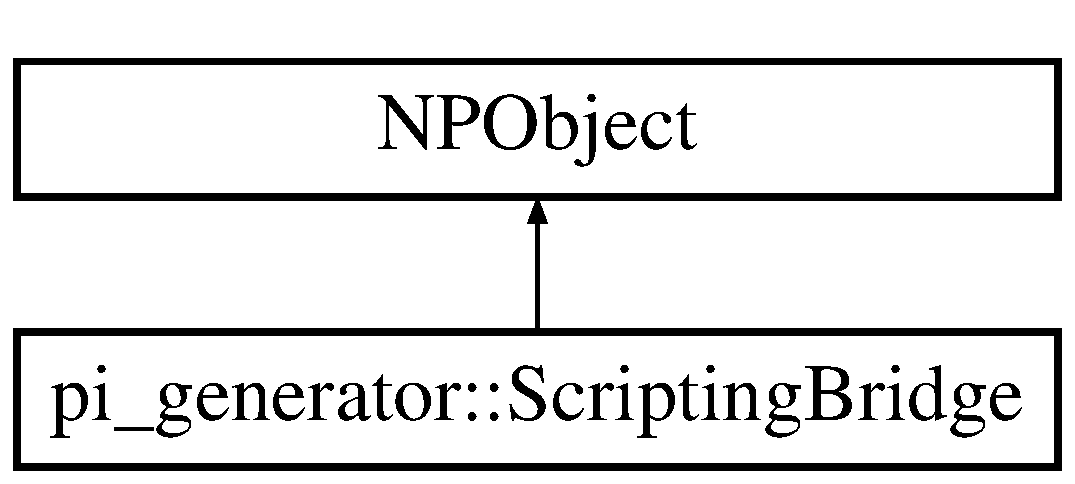
\includegraphics[height=2cm]{classpi__generator_1_1_scripting_bridge}
\end{center}
\end{figure}
\subsection*{Public Types}
\begin{DoxyCompactItemize}
\item 
typedef bool(ScriptingBridge::$\ast$ \hyperlink{classpi__generator_1_1_scripting_bridge_a48f5f7b0dfb3daabcdbfb3f7b667fd39}{Method} )(const \hyperlink{struct___n_p_variant}{NPVariant} $\ast$args, uint32\_\-t arg\_\-count, \hyperlink{struct___n_p_variant}{NPVariant} $\ast$result)
\item 
typedef bool(ScriptingBridge::$\ast$ \hyperlink{classpi__generator_1_1_scripting_bridge_abcd8cffa7f26f348e68cde316038245f}{Property} )(\hyperlink{struct___n_p_variant}{NPVariant} $\ast$result)
\end{DoxyCompactItemize}
\subsection*{Public Member Functions}
\begin{DoxyCompactItemize}
\item 
\hyperlink{classpi__generator_1_1_scripting_bridge_abcc778b6a4c482dff1ed271d7e776e42}{ScriptingBridge} (\hyperlink{struct___n_p_p}{NPP} npp)
\item 
virtual \hyperlink{classpi__generator_1_1_scripting_bridge_a605567080f40ddb9a6c2fa4ea9f2e876}{$\sim$ScriptingBridge} ()
\item 
virtual void \hyperlink{classpi__generator_1_1_scripting_bridge_a581ae88aa4acbefc30ae563452ab2fd5}{Invalidate} ()
\item 
virtual bool \hyperlink{classpi__generator_1_1_scripting_bridge_aaa99f91c8ced5df6fac0700516cdd058}{HasMethod} (\hyperlink{npruntime_8h_a3ce51391e08bd3e24128c342b1d055b9}{NPIdentifier} name)
\item 
virtual bool \hyperlink{classpi__generator_1_1_scripting_bridge_a3518781037308ae1d63bcdf5cc77a3de}{Invoke} (\hyperlink{npruntime_8h_a3ce51391e08bd3e24128c342b1d055b9}{NPIdentifier} name, const \hyperlink{struct___n_p_variant}{NPVariant} $\ast$args, uint32\_\-t arg\_\-count, \hyperlink{struct___n_p_variant}{NPVariant} $\ast$result)
\item 
virtual bool \hyperlink{classpi__generator_1_1_scripting_bridge_a0589fe559ec8b9297e37239233e238be}{InvokeDefault} (const \hyperlink{struct___n_p_variant}{NPVariant} $\ast$args, uint32\_\-t arg\_\-count, \hyperlink{struct___n_p_variant}{NPVariant} $\ast$result)
\item 
virtual bool \hyperlink{classpi__generator_1_1_scripting_bridge_a55f52d9e5e377367881e919db10b019f}{HasProperty} (\hyperlink{npruntime_8h_a3ce51391e08bd3e24128c342b1d055b9}{NPIdentifier} name)
\item 
virtual bool \hyperlink{classpi__generator_1_1_scripting_bridge_ab97693ce171c216783e79debb3b192cc}{GetProperty} (\hyperlink{npruntime_8h_a3ce51391e08bd3e24128c342b1d055b9}{NPIdentifier} name, \hyperlink{struct___n_p_variant}{NPVariant} $\ast$result)
\item 
virtual bool \hyperlink{classpi__generator_1_1_scripting_bridge_aa87ffdeb58a36a1e352814132d4a020a}{SetProperty} (\hyperlink{npruntime_8h_a3ce51391e08bd3e24128c342b1d055b9}{NPIdentifier} name, const \hyperlink{struct___n_p_variant}{NPVariant} $\ast$value)
\item 
virtual bool \hyperlink{classpi__generator_1_1_scripting_bridge_ab1a46993e1a36b9857d48776f7085aa2}{RemoveProperty} (\hyperlink{npruntime_8h_a3ce51391e08bd3e24128c342b1d055b9}{NPIdentifier} name)
\item 
bool \hyperlink{classpi__generator_1_1_scripting_bridge_afcd2c9c3e990cae2d713e8bb5d84048d}{Paint} (const \hyperlink{struct___n_p_variant}{NPVariant} $\ast$args, uint32\_\-t arg\_\-count, \hyperlink{struct___n_p_variant}{NPVariant} $\ast$result)
\end{DoxyCompactItemize}
\subsection*{Static Public Member Functions}
\begin{DoxyCompactItemize}
\item 
static bool \hyperlink{classpi__generator_1_1_scripting_bridge_a76184c7bc22d728d207e275b5f980d67}{InitializeIdentifiers} ()
\end{DoxyCompactItemize}
\subsection*{Static Public Attributes}
\begin{DoxyCompactItemize}
\item 
static \hyperlink{struct_n_p_class}{NPClass} \hyperlink{classpi__generator_1_1_scripting_bridge_a1756e8dff7625cda7697f3e9725ede25}{np\_\-class}
\end{DoxyCompactItemize}


\subsection{Detailed Description}


Definition at line 23 of file scripting\_\-bridge.h.



\subsection{Member Typedef Documentation}
\hypertarget{classpi__generator_1_1_scripting_bridge_a48f5f7b0dfb3daabcdbfb3f7b667fd39}{
\index{pi\_\-generator::ScriptingBridge@{pi\_\-generator::ScriptingBridge}!Method@{Method}}
\index{Method@{Method}!pi_generator::ScriptingBridge@{pi\_\-generator::ScriptingBridge}}
\subsubsection[{Method}]{\setlength{\rightskip}{0pt plus 5cm}typedef bool(ScriptingBridge::$\ast$ {\bf pi\_\-generator::ScriptingBridge::Method})(const {\bf NPVariant} $\ast$args, uint32\_\-t arg\_\-count, {\bf NPVariant} $\ast$result)}}
\label{classpi__generator_1_1_scripting_bridge_a48f5f7b0dfb3daabcdbfb3f7b667fd39}


Definition at line 25 of file scripting\_\-bridge.h.

\hypertarget{classpi__generator_1_1_scripting_bridge_abcd8cffa7f26f348e68cde316038245f}{
\index{pi\_\-generator::ScriptingBridge@{pi\_\-generator::ScriptingBridge}!Property@{Property}}
\index{Property@{Property}!pi_generator::ScriptingBridge@{pi\_\-generator::ScriptingBridge}}
\subsubsection[{Property}]{\setlength{\rightskip}{0pt plus 5cm}typedef bool(ScriptingBridge::$\ast$ {\bf pi\_\-generator::ScriptingBridge::Property})({\bf NPVariant} $\ast$result)}}
\label{classpi__generator_1_1_scripting_bridge_abcd8cffa7f26f348e68cde316038245f}


Definition at line 28 of file scripting\_\-bridge.h.



\subsection{Constructor \& Destructor Documentation}
\hypertarget{classpi__generator_1_1_scripting_bridge_abcc778b6a4c482dff1ed271d7e776e42}{
\index{pi\_\-generator::ScriptingBridge@{pi\_\-generator::ScriptingBridge}!ScriptingBridge@{ScriptingBridge}}
\index{ScriptingBridge@{ScriptingBridge}!pi_generator::ScriptingBridge@{pi\_\-generator::ScriptingBridge}}
\subsubsection[{ScriptingBridge}]{\setlength{\rightskip}{0pt plus 5cm}pi\_\-generator::ScriptingBridge::ScriptingBridge ({\bf NPP} {\em npp})\hspace{0.3cm}{\ttfamily  \mbox{[}inline, explicit\mbox{]}}}}
\label{classpi__generator_1_1_scripting_bridge_abcc778b6a4c482dff1ed271d7e776e42}


Definition at line 30 of file scripting\_\-bridge.h.

\hypertarget{classpi__generator_1_1_scripting_bridge_a605567080f40ddb9a6c2fa4ea9f2e876}{
\index{pi\_\-generator::ScriptingBridge@{pi\_\-generator::ScriptingBridge}!$\sim$ScriptingBridge@{$\sim$ScriptingBridge}}
\index{$\sim$ScriptingBridge@{$\sim$ScriptingBridge}!pi_generator::ScriptingBridge@{pi\_\-generator::ScriptingBridge}}
\subsubsection[{$\sim$ScriptingBridge}]{\setlength{\rightskip}{0pt plus 5cm}pi\_\-generator::ScriptingBridge::$\sim$ScriptingBridge ()\hspace{0.3cm}{\ttfamily  \mbox{[}virtual\mbox{]}}}}
\label{classpi__generator_1_1_scripting_bridge_a605567080f40ddb9a6c2fa4ea9f2e876}


Definition at line 43 of file scripting\_\-bridge.cc.



\subsection{Member Function Documentation}
\hypertarget{classpi__generator_1_1_scripting_bridge_ab97693ce171c216783e79debb3b192cc}{
\index{pi\_\-generator::ScriptingBridge@{pi\_\-generator::ScriptingBridge}!GetProperty@{GetProperty}}
\index{GetProperty@{GetProperty}!pi_generator::ScriptingBridge@{pi\_\-generator::ScriptingBridge}}
\subsubsection[{GetProperty}]{\setlength{\rightskip}{0pt plus 5cm}bool pi\_\-generator::ScriptingBridge::GetProperty ({\bf NPIdentifier} {\em name}, \/  {\bf NPVariant} $\ast$ {\em result})\hspace{0.3cm}{\ttfamily  \mbox{[}virtual\mbox{]}}}}
\label{classpi__generator_1_1_scripting_bridge_ab97693ce171c216783e79debb3b192cc}


Definition at line 64 of file scripting\_\-bridge.cc.

\hypertarget{classpi__generator_1_1_scripting_bridge_aaa99f91c8ced5df6fac0700516cdd058}{
\index{pi\_\-generator::ScriptingBridge@{pi\_\-generator::ScriptingBridge}!HasMethod@{HasMethod}}
\index{HasMethod@{HasMethod}!pi_generator::ScriptingBridge@{pi\_\-generator::ScriptingBridge}}
\subsubsection[{HasMethod}]{\setlength{\rightskip}{0pt plus 5cm}bool pi\_\-generator::ScriptingBridge::HasMethod ({\bf NPIdentifier} {\em name})\hspace{0.3cm}{\ttfamily  \mbox{[}virtual\mbox{]}}}}
\label{classpi__generator_1_1_scripting_bridge_aaa99f91c8ced5df6fac0700516cdd058}


Definition at line 48 of file scripting\_\-bridge.cc.

\hypertarget{classpi__generator_1_1_scripting_bridge_a55f52d9e5e377367881e919db10b019f}{
\index{pi\_\-generator::ScriptingBridge@{pi\_\-generator::ScriptingBridge}!HasProperty@{HasProperty}}
\index{HasProperty@{HasProperty}!pi_generator::ScriptingBridge@{pi\_\-generator::ScriptingBridge}}
\subsubsection[{HasProperty}]{\setlength{\rightskip}{0pt plus 5cm}bool pi\_\-generator::ScriptingBridge::HasProperty ({\bf NPIdentifier} {\em name})\hspace{0.3cm}{\ttfamily  \mbox{[}virtual\mbox{]}}}}
\label{classpi__generator_1_1_scripting_bridge_a55f52d9e5e377367881e919db10b019f}


Definition at line 56 of file scripting\_\-bridge.cc.

\hypertarget{classpi__generator_1_1_scripting_bridge_a76184c7bc22d728d207e275b5f980d67}{
\index{pi\_\-generator::ScriptingBridge@{pi\_\-generator::ScriptingBridge}!InitializeIdentifiers@{InitializeIdentifiers}}
\index{InitializeIdentifiers@{InitializeIdentifiers}!pi_generator::ScriptingBridge@{pi\_\-generator::ScriptingBridge}}
\subsubsection[{InitializeIdentifiers}]{\setlength{\rightskip}{0pt plus 5cm}bool pi\_\-generator::ScriptingBridge::InitializeIdentifiers ()\hspace{0.3cm}{\ttfamily  \mbox{[}static\mbox{]}}}}
\label{classpi__generator_1_1_scripting_bridge_a76184c7bc22d728d207e275b5f980d67}


Definition at line 22 of file scripting\_\-bridge.cc.

\hypertarget{classpi__generator_1_1_scripting_bridge_a581ae88aa4acbefc30ae563452ab2fd5}{
\index{pi\_\-generator::ScriptingBridge@{pi\_\-generator::ScriptingBridge}!Invalidate@{Invalidate}}
\index{Invalidate@{Invalidate}!pi_generator::ScriptingBridge@{pi\_\-generator::ScriptingBridge}}
\subsubsection[{Invalidate}]{\setlength{\rightskip}{0pt plus 5cm}void pi\_\-generator::ScriptingBridge::Invalidate ()\hspace{0.3cm}{\ttfamily  \mbox{[}virtual\mbox{]}}}}
\label{classpi__generator_1_1_scripting_bridge_a581ae88aa4acbefc30ae563452ab2fd5}


Definition at line 110 of file scripting\_\-bridge.cc.

\hypertarget{classpi__generator_1_1_scripting_bridge_a3518781037308ae1d63bcdf5cc77a3de}{
\index{pi\_\-generator::ScriptingBridge@{pi\_\-generator::ScriptingBridge}!Invoke@{Invoke}}
\index{Invoke@{Invoke}!pi_generator::ScriptingBridge@{pi\_\-generator::ScriptingBridge}}
\subsubsection[{Invoke}]{\setlength{\rightskip}{0pt plus 5cm}bool pi\_\-generator::ScriptingBridge::Invoke ({\bf NPIdentifier} {\em name}, \/  const {\bf NPVariant} $\ast$ {\em args}, \/  uint32\_\-t {\em arg\_\-count}, \/  {\bf NPVariant} $\ast$ {\em result})\hspace{0.3cm}{\ttfamily  \mbox{[}virtual\mbox{]}}}}
\label{classpi__generator_1_1_scripting_bridge_a3518781037308ae1d63bcdf5cc77a3de}


Definition at line 97 of file scripting\_\-bridge.cc.

\hypertarget{classpi__generator_1_1_scripting_bridge_a0589fe559ec8b9297e37239233e238be}{
\index{pi\_\-generator::ScriptingBridge@{pi\_\-generator::ScriptingBridge}!InvokeDefault@{InvokeDefault}}
\index{InvokeDefault@{InvokeDefault}!pi_generator::ScriptingBridge@{pi\_\-generator::ScriptingBridge}}
\subsubsection[{InvokeDefault}]{\setlength{\rightskip}{0pt plus 5cm}bool pi\_\-generator::ScriptingBridge::InvokeDefault (const {\bf NPVariant} $\ast$ {\em args}, \/  uint32\_\-t {\em arg\_\-count}, \/  {\bf NPVariant} $\ast$ {\em result})\hspace{0.3cm}{\ttfamily  \mbox{[}virtual\mbox{]}}}}
\label{classpi__generator_1_1_scripting_bridge_a0589fe559ec8b9297e37239233e238be}


Definition at line 89 of file scripting\_\-bridge.cc.

\hypertarget{classpi__generator_1_1_scripting_bridge_afcd2c9c3e990cae2d713e8bb5d84048d}{
\index{pi\_\-generator::ScriptingBridge@{pi\_\-generator::ScriptingBridge}!Paint@{Paint}}
\index{Paint@{Paint}!pi_generator::ScriptingBridge@{pi\_\-generator::ScriptingBridge}}
\subsubsection[{Paint}]{\setlength{\rightskip}{0pt plus 5cm}bool pi\_\-generator::ScriptingBridge::Paint (const {\bf NPVariant} $\ast$ {\em args}, \/  uint32\_\-t {\em arg\_\-count}, \/  {\bf NPVariant} $\ast$ {\em result})}}
\label{classpi__generator_1_1_scripting_bridge_afcd2c9c3e990cae2d713e8bb5d84048d}


Definition at line 114 of file scripting\_\-bridge.cc.

\hypertarget{classpi__generator_1_1_scripting_bridge_ab1a46993e1a36b9857d48776f7085aa2}{
\index{pi\_\-generator::ScriptingBridge@{pi\_\-generator::ScriptingBridge}!RemoveProperty@{RemoveProperty}}
\index{RemoveProperty@{RemoveProperty}!pi_generator::ScriptingBridge@{pi\_\-generator::ScriptingBridge}}
\subsubsection[{RemoveProperty}]{\setlength{\rightskip}{0pt plus 5cm}bool pi\_\-generator::ScriptingBridge::RemoveProperty ({\bf NPIdentifier} {\em name})\hspace{0.3cm}{\ttfamily  \mbox{[}virtual\mbox{]}}}}
\label{classpi__generator_1_1_scripting_bridge_ab1a46993e1a36b9857d48776f7085aa2}


Definition at line 83 of file scripting\_\-bridge.cc.

\hypertarget{classpi__generator_1_1_scripting_bridge_aa87ffdeb58a36a1e352814132d4a020a}{
\index{pi\_\-generator::ScriptingBridge@{pi\_\-generator::ScriptingBridge}!SetProperty@{SetProperty}}
\index{SetProperty@{SetProperty}!pi_generator::ScriptingBridge@{pi\_\-generator::ScriptingBridge}}
\subsubsection[{SetProperty}]{\setlength{\rightskip}{0pt plus 5cm}bool pi\_\-generator::ScriptingBridge::SetProperty ({\bf NPIdentifier} {\em name}, \/  const {\bf NPVariant} $\ast$ {\em value})\hspace{0.3cm}{\ttfamily  \mbox{[}virtual\mbox{]}}}}
\label{classpi__generator_1_1_scripting_bridge_aa87ffdeb58a36a1e352814132d4a020a}


Definition at line 77 of file scripting\_\-bridge.cc.



\subsection{Member Data Documentation}
\hypertarget{classpi__generator_1_1_scripting_bridge_a1756e8dff7625cda7697f3e9725ede25}{
\index{pi\_\-generator::ScriptingBridge@{pi\_\-generator::ScriptingBridge}!np\_\-class@{np\_\-class}}
\index{np\_\-class@{np\_\-class}!pi_generator::ScriptingBridge@{pi\_\-generator::ScriptingBridge}}
\subsubsection[{np\_\-class}]{\setlength{\rightskip}{0pt plus 5cm}{\bf NPClass} {\bf pi\_\-generator::ScriptingBridge::np\_\-class}\hspace{0.3cm}{\ttfamily  \mbox{[}static\mbox{]}}}}
\label{classpi__generator_1_1_scripting_bridge_a1756e8dff7625cda7697f3e9725ede25}
{\bfseries Initial value:}
\begin{DoxyCode}
 {
  NP_CLASS_STRUCT_VERSION,
  pi_generator::Allocate,
  pi_generator::Deallocate,
  pi_generator::Invalidate,
  pi_generator::HasMethod,
  pi_generator::Invoke,
  pi_generator::InvokeDefault,
  pi_generator::HasProperty,
  pi_generator::GetProperty,
  pi_generator::SetProperty,
  pi_generator::RemoveProperty
}
\end{DoxyCode}


Definition at line 51 of file scripting\_\-bridge.h.



The documentation for this class was generated from the following files:\begin{DoxyCompactItemize}
\item 
/home/derek/dev/cell-\/grid-\/game/nacl/crml/crml/test/pi\_\-generator/\hyperlink{test_2pi__generator_2scripting__bridge_8h}{scripting\_\-bridge.h}\item 
/home/derek/dev/cell-\/grid-\/game/nacl/crml/crml/core/\hyperlink{core_2scripting__bridge_8cc}{scripting\_\-bridge.cc}\item 
/home/derek/dev/cell-\/grid-\/game/nacl/crml/crml/test/pi\_\-generator/\hyperlink{test_2pi__generator_2scripting__bridge_8cc}{scripting\_\-bridge.cc}\end{DoxyCompactItemize}

\hypertarget{classtumbler_1_1_scripting_bridge}{
\section{tumbler::ScriptingBridge Class Reference}
\label{classtumbler_1_1_scripting_bridge}\index{tumbler::ScriptingBridge@{tumbler::ScriptingBridge}}
}


{\ttfamily \#include $<$scripting\_\-bridge.h$>$}

\subsection*{Public Types}
\begin{DoxyCompactItemize}
\item 
typedef bool(ScriptingBridge::$\ast$ \hyperlink{classtumbler_1_1_scripting_bridge_addb1badb0e891b38c6d90767342b5bb3}{Method} )(const NPVariant $\ast$args, uint32\_\-t arg\_\-count, NPVariant $\ast$result)
\item 
typedef bool(ScriptingBridge::$\ast$ \hyperlink{classtumbler_1_1_scripting_bridge_ad7507ce0e5c8f49fde790c743447f3c3}{Property} )(NPVariant $\ast$result)
\end{DoxyCompactItemize}
\subsection*{Public Member Functions}
\begin{DoxyCompactItemize}
\item 
\hyperlink{classtumbler_1_1_scripting_bridge_aa7abb8784b22a793d795e872841b4bac}{ScriptingBridge} (\hyperlink{struct___n_p_p}{NPP} npp)
\item 
virtual \hyperlink{classtumbler_1_1_scripting_bridge_abe0d3eec9a772e0bc7f906cbc432d58d}{$\sim$ScriptingBridge} ()
\item 
virtual void \hyperlink{classtumbler_1_1_scripting_bridge_a79ca9287d682b30670932c235ce025b4}{Invalidate} ()
\item 
virtual bool \hyperlink{classtumbler_1_1_scripting_bridge_acd4789c8a9668e86ad02949ac7e88481}{HasMethod} (NPIdentifier name)
\item 
virtual bool \hyperlink{classtumbler_1_1_scripting_bridge_a70638ad7da4726fb8ccbc6f49868fafc}{Invoke} (NPIdentifier name, const NPVariant $\ast$args, uint32\_\-t arg\_\-count, NPVariant $\ast$result)
\item 
virtual bool \hyperlink{classtumbler_1_1_scripting_bridge_abc3713f16c739bb1c547def1afc5c93c}{InvokeDefault} (const NPVariant $\ast$args, uint32\_\-t arg\_\-count, NPVariant $\ast$result)
\item 
virtual bool \hyperlink{classtumbler_1_1_scripting_bridge_af5fea670d935111ef96b2ecc3adc8576}{HasProperty} (NPIdentifier name)
\item 
virtual bool \hyperlink{classtumbler_1_1_scripting_bridge_a7f8c653d8a5cb632eae37e1d59459c31}{GetProperty} (NPIdentifier name, NPVariant $\ast$result)
\item 
virtual bool \hyperlink{classtumbler_1_1_scripting_bridge_a841486a4fe8e3245dd8d1711e2c72dd3}{SetProperty} (NPIdentifier name, const NPVariant $\ast$value)
\item 
virtual bool \hyperlink{classtumbler_1_1_scripting_bridge_a58c45c6be183d37e0fa26de95b4410a1}{RemoveProperty} (NPIdentifier name)
\item 
bool \hyperlink{classtumbler_1_1_scripting_bridge_ace2d208ee47d10881e48945a1b9deb1e}{GetCameraOrientation} (const NPVariant $\ast$args, uint32\_\-t arg\_\-count, NPVariant $\ast$result)
\item 
bool \hyperlink{classtumbler_1_1_scripting_bridge_a9e3ffd7304dc607ddecad7cb8774009a}{SetCameraOrientation} (const NPVariant $\ast$args, uint32\_\-t arg\_\-count, NPVariant $\ast$value)
\end{DoxyCompactItemize}
\subsection*{Static Public Member Functions}
\begin{DoxyCompactItemize}
\item 
static bool \hyperlink{classtumbler_1_1_scripting_bridge_a9653f59bae05d24f2f319a2764a7ce61}{InitializeIdentifiers} ()
\end{DoxyCompactItemize}
\subsection*{Static Public Attributes}
\begin{DoxyCompactItemize}
\item 
static NPClass \hyperlink{classtumbler_1_1_scripting_bridge_a4cd00d35febde2739ee85287f39981ac}{np\_\-class}
\end{DoxyCompactItemize}


\subsection{Detailed Description}


Definition at line 23 of file scripting\_\-bridge.h.



\subsection{Member Typedef Documentation}
\hypertarget{classtumbler_1_1_scripting_bridge_addb1badb0e891b38c6d90767342b5bb3}{
\index{tumbler::ScriptingBridge@{tumbler::ScriptingBridge}!Method@{Method}}
\index{Method@{Method}!tumbler::ScriptingBridge@{tumbler::ScriptingBridge}}
\subsubsection[{Method}]{\setlength{\rightskip}{0pt plus 5cm}typedef bool(ScriptingBridge::$\ast$ {\bf tumbler::ScriptingBridge::Method})(const NPVariant $\ast$args, uint32\_\-t arg\_\-count, NPVariant $\ast$result)}}
\label{classtumbler_1_1_scripting_bridge_addb1badb0e891b38c6d90767342b5bb3}


Definition at line 25 of file scripting\_\-bridge.h.

\hypertarget{classtumbler_1_1_scripting_bridge_ad7507ce0e5c8f49fde790c743447f3c3}{
\index{tumbler::ScriptingBridge@{tumbler::ScriptingBridge}!Property@{Property}}
\index{Property@{Property}!tumbler::ScriptingBridge@{tumbler::ScriptingBridge}}
\subsubsection[{Property}]{\setlength{\rightskip}{0pt plus 5cm}typedef bool(ScriptingBridge::$\ast$ {\bf tumbler::ScriptingBridge::Property})(NPVariant $\ast$result)}}
\label{classtumbler_1_1_scripting_bridge_ad7507ce0e5c8f49fde790c743447f3c3}


Definition at line 28 of file scripting\_\-bridge.h.



\subsection{Constructor \& Destructor Documentation}
\hypertarget{classtumbler_1_1_scripting_bridge_aa7abb8784b22a793d795e872841b4bac}{
\index{tumbler::ScriptingBridge@{tumbler::ScriptingBridge}!ScriptingBridge@{ScriptingBridge}}
\index{ScriptingBridge@{ScriptingBridge}!tumbler::ScriptingBridge@{tumbler::ScriptingBridge}}
\subsubsection[{ScriptingBridge}]{\setlength{\rightskip}{0pt plus 5cm}tumbler::ScriptingBridge::ScriptingBridge ({\bf NPP} {\em npp})\hspace{0.3cm}{\ttfamily  \mbox{[}explicit\mbox{]}}}}
\label{classtumbler_1_1_scripting_bridge_aa7abb8784b22a793d795e872841b4bac}


Definition at line 54 of file scripting\_\-bridge.cc.

\hypertarget{classtumbler_1_1_scripting_bridge_abe0d3eec9a772e0bc7f906cbc432d58d}{
\index{tumbler::ScriptingBridge@{tumbler::ScriptingBridge}!$\sim$ScriptingBridge@{$\sim$ScriptingBridge}}
\index{$\sim$ScriptingBridge@{$\sim$ScriptingBridge}!tumbler::ScriptingBridge@{tumbler::ScriptingBridge}}
\subsubsection[{$\sim$ScriptingBridge}]{\setlength{\rightskip}{0pt plus 5cm}tumbler::ScriptingBridge::$\sim$ScriptingBridge ()\hspace{0.3cm}{\ttfamily  \mbox{[}virtual\mbox{]}}}}
\label{classtumbler_1_1_scripting_bridge_abe0d3eec9a772e0bc7f906cbc432d58d}


Definition at line 60 of file scripting\_\-bridge.cc.



\subsection{Member Function Documentation}
\hypertarget{classtumbler_1_1_scripting_bridge_ace2d208ee47d10881e48945a1b9deb1e}{
\index{tumbler::ScriptingBridge@{tumbler::ScriptingBridge}!GetCameraOrientation@{GetCameraOrientation}}
\index{GetCameraOrientation@{GetCameraOrientation}!tumbler::ScriptingBridge@{tumbler::ScriptingBridge}}
\subsubsection[{GetCameraOrientation}]{\setlength{\rightskip}{0pt plus 5cm}bool tumbler::ScriptingBridge::GetCameraOrientation (const NPVariant $\ast$ {\em args}, \/  uint32\_\-t {\em arg\_\-count}, \/  NPVariant $\ast$ {\em result})}}
\label{classtumbler_1_1_scripting_bridge_ace2d208ee47d10881e48945a1b9deb1e}


Definition at line 133 of file scripting\_\-bridge.cc.

\hypertarget{classtumbler_1_1_scripting_bridge_a7f8c653d8a5cb632eae37e1d59459c31}{
\index{tumbler::ScriptingBridge@{tumbler::ScriptingBridge}!GetProperty@{GetProperty}}
\index{GetProperty@{GetProperty}!tumbler::ScriptingBridge@{tumbler::ScriptingBridge}}
\subsubsection[{GetProperty}]{\setlength{\rightskip}{0pt plus 5cm}bool tumbler::ScriptingBridge::GetProperty (NPIdentifier {\em name}, \/  NPVariant $\ast$ {\em result})\hspace{0.3cm}{\ttfamily  \mbox{[}virtual\mbox{]}}}}
\label{classtumbler_1_1_scripting_bridge_a7f8c653d8a5cb632eae37e1d59459c31}


Definition at line 84 of file scripting\_\-bridge.cc.

\hypertarget{classtumbler_1_1_scripting_bridge_acd4789c8a9668e86ad02949ac7e88481}{
\index{tumbler::ScriptingBridge@{tumbler::ScriptingBridge}!HasMethod@{HasMethod}}
\index{HasMethod@{HasMethod}!tumbler::ScriptingBridge@{tumbler::ScriptingBridge}}
\subsubsection[{HasMethod}]{\setlength{\rightskip}{0pt plus 5cm}bool tumbler::ScriptingBridge::HasMethod (NPIdentifier {\em name})\hspace{0.3cm}{\ttfamily  \mbox{[}virtual\mbox{]}}}}
\label{classtumbler_1_1_scripting_bridge_acd4789c8a9668e86ad02949ac7e88481}


Definition at line 68 of file scripting\_\-bridge.cc.

\hypertarget{classtumbler_1_1_scripting_bridge_af5fea670d935111ef96b2ecc3adc8576}{
\index{tumbler::ScriptingBridge@{tumbler::ScriptingBridge}!HasProperty@{HasProperty}}
\index{HasProperty@{HasProperty}!tumbler::ScriptingBridge@{tumbler::ScriptingBridge}}
\subsubsection[{HasProperty}]{\setlength{\rightskip}{0pt plus 5cm}bool tumbler::ScriptingBridge::HasProperty (NPIdentifier {\em name})\hspace{0.3cm}{\ttfamily  \mbox{[}virtual\mbox{]}}}}
\label{classtumbler_1_1_scripting_bridge_af5fea670d935111ef96b2ecc3adc8576}


Definition at line 76 of file scripting\_\-bridge.cc.

\hypertarget{classtumbler_1_1_scripting_bridge_a9653f59bae05d24f2f319a2764a7ce61}{
\index{tumbler::ScriptingBridge@{tumbler::ScriptingBridge}!InitializeIdentifiers@{InitializeIdentifiers}}
\index{InitializeIdentifiers@{InitializeIdentifiers}!tumbler::ScriptingBridge@{tumbler::ScriptingBridge}}
\subsubsection[{InitializeIdentifiers}]{\setlength{\rightskip}{0pt plus 5cm}bool tumbler::ScriptingBridge::InitializeIdentifiers ()\hspace{0.3cm}{\ttfamily  \mbox{[}static\mbox{]}}}}
\label{classtumbler_1_1_scripting_bridge_a9653f59bae05d24f2f319a2764a7ce61}


Definition at line 28 of file scripting\_\-bridge.cc.

\hypertarget{classtumbler_1_1_scripting_bridge_a79ca9287d682b30670932c235ce025b4}{
\index{tumbler::ScriptingBridge@{tumbler::ScriptingBridge}!Invalidate@{Invalidate}}
\index{Invalidate@{Invalidate}!tumbler::ScriptingBridge@{tumbler::ScriptingBridge}}
\subsubsection[{Invalidate}]{\setlength{\rightskip}{0pt plus 5cm}void tumbler::ScriptingBridge::Invalidate ()\hspace{0.3cm}{\ttfamily  \mbox{[}virtual\mbox{]}}}}
\label{classtumbler_1_1_scripting_bridge_a79ca9287d682b30670932c235ce025b4}


Definition at line 129 of file scripting\_\-bridge.cc.

\hypertarget{classtumbler_1_1_scripting_bridge_a70638ad7da4726fb8ccbc6f49868fafc}{
\index{tumbler::ScriptingBridge@{tumbler::ScriptingBridge}!Invoke@{Invoke}}
\index{Invoke@{Invoke}!tumbler::ScriptingBridge@{tumbler::ScriptingBridge}}
\subsubsection[{Invoke}]{\setlength{\rightskip}{0pt plus 5cm}bool tumbler::ScriptingBridge::Invoke (NPIdentifier {\em name}, \/  const NPVariant $\ast$ {\em args}, \/  uint32\_\-t {\em arg\_\-count}, \/  NPVariant $\ast$ {\em result})\hspace{0.3cm}{\ttfamily  \mbox{[}virtual\mbox{]}}}}
\label{classtumbler_1_1_scripting_bridge_a70638ad7da4726fb8ccbc6f49868fafc}


Definition at line 118 of file scripting\_\-bridge.cc.

\hypertarget{classtumbler_1_1_scripting_bridge_abc3713f16c739bb1c547def1afc5c93c}{
\index{tumbler::ScriptingBridge@{tumbler::ScriptingBridge}!InvokeDefault@{InvokeDefault}}
\index{InvokeDefault@{InvokeDefault}!tumbler::ScriptingBridge@{tumbler::ScriptingBridge}}
\subsubsection[{InvokeDefault}]{\setlength{\rightskip}{0pt plus 5cm}bool tumbler::ScriptingBridge::InvokeDefault (const NPVariant $\ast$ {\em args}, \/  uint32\_\-t {\em arg\_\-count}, \/  NPVariant $\ast$ {\em result})\hspace{0.3cm}{\ttfamily  \mbox{[}virtual\mbox{]}}}}
\label{classtumbler_1_1_scripting_bridge_abc3713f16c739bb1c547def1afc5c93c}


Definition at line 110 of file scripting\_\-bridge.cc.

\hypertarget{classtumbler_1_1_scripting_bridge_a58c45c6be183d37e0fa26de95b4410a1}{
\index{tumbler::ScriptingBridge@{tumbler::ScriptingBridge}!RemoveProperty@{RemoveProperty}}
\index{RemoveProperty@{RemoveProperty}!tumbler::ScriptingBridge@{tumbler::ScriptingBridge}}
\subsubsection[{RemoveProperty}]{\setlength{\rightskip}{0pt plus 5cm}bool tumbler::ScriptingBridge::RemoveProperty (NPIdentifier {\em name})\hspace{0.3cm}{\ttfamily  \mbox{[}virtual\mbox{]}}}}
\label{classtumbler_1_1_scripting_bridge_a58c45c6be183d37e0fa26de95b4410a1}


Definition at line 104 of file scripting\_\-bridge.cc.

\hypertarget{classtumbler_1_1_scripting_bridge_a9e3ffd7304dc607ddecad7cb8774009a}{
\index{tumbler::ScriptingBridge@{tumbler::ScriptingBridge}!SetCameraOrientation@{SetCameraOrientation}}
\index{SetCameraOrientation@{SetCameraOrientation}!tumbler::ScriptingBridge@{tumbler::ScriptingBridge}}
\subsubsection[{SetCameraOrientation}]{\setlength{\rightskip}{0pt plus 5cm}bool tumbler::ScriptingBridge::SetCameraOrientation (const NPVariant $\ast$ {\em args}, \/  uint32\_\-t {\em arg\_\-count}, \/  NPVariant $\ast$ {\em value})}}
\label{classtumbler_1_1_scripting_bridge_a9e3ffd7304dc607ddecad7cb8774009a}


Definition at line 171 of file scripting\_\-bridge.cc.

\hypertarget{classtumbler_1_1_scripting_bridge_a841486a4fe8e3245dd8d1711e2c72dd3}{
\index{tumbler::ScriptingBridge@{tumbler::ScriptingBridge}!SetProperty@{SetProperty}}
\index{SetProperty@{SetProperty}!tumbler::ScriptingBridge@{tumbler::ScriptingBridge}}
\subsubsection[{SetProperty}]{\setlength{\rightskip}{0pt plus 5cm}bool tumbler::ScriptingBridge::SetProperty (NPIdentifier {\em name}, \/  const NPVariant $\ast$ {\em value})\hspace{0.3cm}{\ttfamily  \mbox{[}virtual\mbox{]}}}}
\label{classtumbler_1_1_scripting_bridge_a841486a4fe8e3245dd8d1711e2c72dd3}


Definition at line 98 of file scripting\_\-bridge.cc.



\subsection{Member Data Documentation}
\hypertarget{classtumbler_1_1_scripting_bridge_a4cd00d35febde2739ee85287f39981ac}{
\index{tumbler::ScriptingBridge@{tumbler::ScriptingBridge}!np\_\-class@{np\_\-class}}
\index{np\_\-class@{np\_\-class}!tumbler::ScriptingBridge@{tumbler::ScriptingBridge}}
\subsubsection[{np\_\-class}]{\setlength{\rightskip}{0pt plus 5cm}NPClass {\bf tumbler::ScriptingBridge::np\_\-class}\hspace{0.3cm}{\ttfamily  \mbox{[}static\mbox{]}}}}
\label{classtumbler_1_1_scripting_bridge_a4cd00d35febde2739ee85287f39981ac}
{\bfseries Initial value:}
\begin{DoxyCode}
 {
  NP_CLASS_STRUCT_VERSION,
  tumbler::Allocate,
  tumbler::Deallocate,
  tumbler::Invalidate,
  tumbler::HasMethod,
  tumbler::Invoke,
  tumbler::InvokeDefault,
  tumbler::HasProperty,
  tumbler::GetProperty,
  tumbler::SetProperty,
  tumbler::RemoveProperty
}
\end{DoxyCode}


Definition at line 51 of file scripting\_\-bridge.h.



The documentation for this class was generated from the following files:\begin{DoxyCompactItemize}
\item 
/home/derek/dev/cell-\/grid-\/game/nacl/crml/crml/lib/tumbler/\hyperlink{lib_2tumbler_2scripting__bridge_8h}{scripting\_\-bridge.h}\item 
/home/derek/dev/cell-\/grid-\/game/nacl/crml/crml/lib/tumbler/\hyperlink{lib_2tumbler_2scripting__bridge_8cc}{scripting\_\-bridge.cc}\end{DoxyCompactItemize}

\hypertarget{struct_test_object}{
\section{TestObject Struct Reference}
\label{struct_test_object}\index{TestObject@{TestObject}}
}


{\ttfamily \#include $<$test\_\-object.h$>$}

\subsection*{Public Attributes}
\begin{DoxyCompactItemize}
\item 
NPObject \hyperlink{struct_test_object_a23d7a50afe1b29f85b5d663cbfc763b2}{header}
\item 
NPObject $\ast$ \hyperlink{struct_test_object_a375c492938a3abf12d768b8578549861}{test\_\-object}
\end{DoxyCompactItemize}


\subsection{Detailed Description}


Definition at line 32 of file test\_\-object.h.



\subsection{Member Data Documentation}
\hypertarget{struct_test_object_a23d7a50afe1b29f85b5d663cbfc763b2}{
\index{TestObject@{TestObject}!header@{header}}
\index{header@{header}!TestObject@{TestObject}}
\subsubsection[{header}]{\setlength{\rightskip}{0pt plus 5cm}NPObject {\bf TestObject::header}}}
\label{struct_test_object_a23d7a50afe1b29f85b5d663cbfc763b2}


Definition at line 33 of file test\_\-object.h.

\hypertarget{struct_test_object_a375c492938a3abf12d768b8578549861}{
\index{TestObject@{TestObject}!test\_\-object@{test\_\-object}}
\index{test\_\-object@{test\_\-object}!TestObject@{TestObject}}
\subsubsection[{test\_\-object}]{\setlength{\rightskip}{0pt plus 5cm}NPObject $\ast$ {\bf TestObject::test\_\-object}}}
\label{struct_test_object_a375c492938a3abf12d768b8578549861}


Definition at line 34 of file test\_\-object.h.



The documentation for this struct was generated from the following files:\begin{DoxyCompactItemize}
\item 
/home/derek/dev/cell-\/grid-\/game/nacl/crml/crml/sys/\hyperlink{sys_2test__object_8h}{test\_\-object.h}\item 
/home/derek/dev/cell-\/grid-\/game/nacl/crml/crml/test/\hyperlink{test_2test__object_8h}{test\_\-object.h}\end{DoxyCompactItemize}

\hypertarget{classtumbler_1_1_tumbler}{
\section{tumbler::Tumbler Class Reference}
\label{classtumbler_1_1_tumbler}\index{tumbler::Tumbler@{tumbler::Tumbler}}
}


{\ttfamily \#include $<$tumbler.h$>$}

\subsection*{Public Member Functions}
\begin{DoxyCompactItemize}
\item 
\hyperlink{classtumbler_1_1_tumbler_a4f5dd0baa068ccb8214b0e477f7cd94b}{Tumbler} (NPP npp)
\item 
\hyperlink{classtumbler_1_1_tumbler_a80349e180aa825c15d63bada00c6e9a8}{$\sim$Tumbler} ()
\item 
NPObject $\ast$ \hyperlink{classtumbler_1_1_tumbler_ad438453c62d1edcbdd5cb39a38143a0b}{GetScriptableObject} ()
\item 
NPError \hyperlink{classtumbler_1_1_tumbler_a6aba2f3cfa10be35c0a789924343b1b0}{SetWindow} (const NPWindow \&window)
\item 
void \hyperlink{classtumbler_1_1_tumbler_ab721f5f95ce020ce6680033771ed4577}{PostRedrawNotification} ()
\item 
bool \hyperlink{classtumbler_1_1_tumbler_a8da0b0b0e85708487c55f6ca5c999da1}{DrawSelf} ()
\item 
bool \hyperlink{classtumbler_1_1_tumbler_a5e01d6cde9baab4e5c2aa4b834733bf2}{GetCameraOrientation} (float $\ast$orientation) const 
\item 
bool \hyperlink{classtumbler_1_1_tumbler_a2657d32f15492fc56406d1750172ca8c}{SetCameraOrientation} (const float $\ast$orientation)
\end{DoxyCompactItemize}


\subsection{Detailed Description}


Definition at line 38 of file tumbler.h.



\subsection{Constructor \& Destructor Documentation}
\hypertarget{classtumbler_1_1_tumbler_a4f5dd0baa068ccb8214b0e477f7cd94b}{
\index{tumbler::Tumbler@{tumbler::Tumbler}!Tumbler@{Tumbler}}
\index{Tumbler@{Tumbler}!tumbler::Tumbler@{tumbler::Tumbler}}
\subsubsection[{Tumbler}]{\setlength{\rightskip}{0pt plus 5cm}tumbler::Tumbler::Tumbler (NPP {\em npp})\hspace{0.3cm}{\ttfamily  \mbox{[}explicit\mbox{]}}}}
\label{classtumbler_1_1_tumbler_a4f5dd0baa068ccb8214b0e477f7cd94b}


Definition at line 38 of file tumbler.cc.

\hypertarget{classtumbler_1_1_tumbler_a80349e180aa825c15d63bada00c6e9a8}{
\index{tumbler::Tumbler@{tumbler::Tumbler}!$\sim$Tumbler@{$\sim$Tumbler}}
\index{$\sim$Tumbler@{$\sim$Tumbler}!tumbler::Tumbler@{tumbler::Tumbler}}
\subsubsection[{$\sim$Tumbler}]{\setlength{\rightskip}{0pt plus 5cm}tumbler::Tumbler::$\sim$Tumbler ()}}
\label{classtumbler_1_1_tumbler_a80349e180aa825c15d63bada00c6e9a8}


Definition at line 48 of file tumbler.cc.



\subsection{Member Function Documentation}
\hypertarget{classtumbler_1_1_tumbler_a8da0b0b0e85708487c55f6ca5c999da1}{
\index{tumbler::Tumbler@{tumbler::Tumbler}!DrawSelf@{DrawSelf}}
\index{DrawSelf@{DrawSelf}!tumbler::Tumbler@{tumbler::Tumbler}}
\subsubsection[{DrawSelf}]{\setlength{\rightskip}{0pt plus 5cm}bool tumbler::Tumbler::DrawSelf ()}}
\label{classtumbler_1_1_tumbler_a8da0b0b0e85708487c55f6ca5c999da1}


Definition at line 90 of file tumbler.cc.

\hypertarget{classtumbler_1_1_tumbler_a5e01d6cde9baab4e5c2aa4b834733bf2}{
\index{tumbler::Tumbler@{tumbler::Tumbler}!GetCameraOrientation@{GetCameraOrientation}}
\index{GetCameraOrientation@{GetCameraOrientation}!tumbler::Tumbler@{tumbler::Tumbler}}
\subsubsection[{GetCameraOrientation}]{\setlength{\rightskip}{0pt plus 5cm}bool tumbler::Tumbler::GetCameraOrientation (float $\ast$ {\em orientation}) const}}
\label{classtumbler_1_1_tumbler_a5e01d6cde9baab4e5c2aa4b834733bf2}


Definition at line 109 of file tumbler.cc.

\hypertarget{classtumbler_1_1_tumbler_ad438453c62d1edcbdd5cb39a38143a0b}{
\index{tumbler::Tumbler@{tumbler::Tumbler}!GetScriptableObject@{GetScriptableObject}}
\index{GetScriptableObject@{GetScriptableObject}!tumbler::Tumbler@{tumbler::Tumbler}}
\subsubsection[{GetScriptableObject}]{\setlength{\rightskip}{0pt plus 5cm}NPObject $\ast$ tumbler::Tumbler::GetScriptableObject ()}}
\label{classtumbler_1_1_tumbler_ad438453c62d1edcbdd5cb39a38143a0b}


Definition at line 60 of file tumbler.cc.

\hypertarget{classtumbler_1_1_tumbler_ab721f5f95ce020ce6680033771ed4577}{
\index{tumbler::Tumbler@{tumbler::Tumbler}!PostRedrawNotification@{PostRedrawNotification}}
\index{PostRedrawNotification@{PostRedrawNotification}!tumbler::Tumbler@{tumbler::Tumbler}}
\subsubsection[{PostRedrawNotification}]{\setlength{\rightskip}{0pt plus 5cm}void tumbler::Tumbler::PostRedrawNotification ()}}
\label{classtumbler_1_1_tumbler_ab721f5f95ce020ce6680033771ed4577}


Definition at line 86 of file tumbler.cc.

\hypertarget{classtumbler_1_1_tumbler_a2657d32f15492fc56406d1750172ca8c}{
\index{tumbler::Tumbler@{tumbler::Tumbler}!SetCameraOrientation@{SetCameraOrientation}}
\index{SetCameraOrientation@{SetCameraOrientation}!tumbler::Tumbler@{tumbler::Tumbler}}
\subsubsection[{SetCameraOrientation}]{\setlength{\rightskip}{0pt plus 5cm}bool tumbler::Tumbler::SetCameraOrientation (const float $\ast$ {\em orientation})}}
\label{classtumbler_1_1_tumbler_a2657d32f15492fc56406d1750172ca8c}


Definition at line 117 of file tumbler.cc.

\hypertarget{classtumbler_1_1_tumbler_a6aba2f3cfa10be35c0a789924343b1b0}{
\index{tumbler::Tumbler@{tumbler::Tumbler}!SetWindow@{SetWindow}}
\index{SetWindow@{SetWindow}!tumbler::Tumbler@{tumbler::Tumbler}}
\subsubsection[{SetWindow}]{\setlength{\rightskip}{0pt plus 5cm}NPError tumbler::Tumbler::SetWindow (const NPWindow \& {\em window})}}
\label{classtumbler_1_1_tumbler_a6aba2f3cfa10be35c0a789924343b1b0}


Definition at line 71 of file tumbler.cc.



The documentation for this class was generated from the following files:\begin{DoxyCompactItemize}
\item 
/home/derek/dev/crml/crml/lib/tumbler/\hyperlink{tumbler_8h}{tumbler.h}\item 
/home/derek/dev/crml/crml/lib/tumbler/\hyperlink{tumbler_8cc}{tumbler.cc}\end{DoxyCompactItemize}

\hypertarget{structtumbler_1_1_tumbler_context3_d}{
\section{tumbler::TumblerContext3D Struct Reference}
\label{structtumbler_1_1_tumbler_context3_d}\index{tumbler::TumblerContext3D@{tumbler::TumblerContext3D}}
}


{\ttfamily \#include $<$tumbler.h$>$}

\subsection*{Public Attributes}
\begin{DoxyCompactItemize}
\item 
void $\ast$ \hyperlink{structtumbler_1_1_tumbler_context3_d_a1274a5b24b002c4e264bc7ee9298e85d}{user\_\-data\_\-}
\end{DoxyCompactItemize}


\subsection{Detailed Description}


Definition at line 34 of file tumbler.h.



\subsection{Member Data Documentation}
\hypertarget{structtumbler_1_1_tumbler_context3_d_a1274a5b24b002c4e264bc7ee9298e85d}{
\index{tumbler::TumblerContext3D@{tumbler::TumblerContext3D}!user\_\-data\_\-@{user\_\-data\_\-}}
\index{user\_\-data\_\-@{user\_\-data\_\-}!tumbler::TumblerContext3D@{tumbler::TumblerContext3D}}
\subsubsection[{user\_\-data\_\-}]{\setlength{\rightskip}{0pt plus 5cm}void$\ast$ {\bf tumbler::TumblerContext3D::user\_\-data\_\-}}}
\label{structtumbler_1_1_tumbler_context3_d_a1274a5b24b002c4e264bc7ee9298e85d}


Definition at line 35 of file tumbler.h.



The documentation for this struct was generated from the following file:\begin{DoxyCompactItemize}
\item 
/home/derek/dev/crml/crml/lib/tumbler/\hyperlink{tumbler_8h}{tumbler.h}\end{DoxyCompactItemize}

\chapter{File Documentation}
\hypertarget{core_8h}{
\section{/home/derek/dev/cell-\/grid-\/game/nacl/crml/crml/core/core.h File Reference}
\label{core_8h}\index{/home/derek/dev/cell-\/grid-\/game/nacl/crml/crml/core/core.h@{/home/derek/dev/cell-\/grid-\/game/nacl/crml/crml/core/core.h}}
}
\subsection*{Classes}
\begin{DoxyCompactItemize}
\item 
class \hyperlink{classcrml_1_1_core}{crml::Core}
\begin{DoxyCompactList}\small\item\em The \hyperlink{classcrml_1_1_core}{Core} object which wires all subsystems and maintains an open channel with javascript. \item\end{DoxyCompactList}\end{DoxyCompactItemize}
\subsection*{Namespaces}
\begin{DoxyCompactItemize}
\item 
namespace \hyperlink{namespacecrml}{crml}
\end{DoxyCompactItemize}

\hypertarget{nacl__macros_8h}{
\section{/home/derek/dev/cell-\/grid-\/game/nacl/crml/crml/core/nacl\_\-macros.h File Reference}
\label{nacl__macros_8h}\index{/home/derek/dev/cell-\/grid-\/game/nacl/crml/crml/core/nacl\_\-macros.h@{/home/derek/dev/cell-\/grid-\/game/nacl/crml/crml/core/nacl\_\-macros.h}}
}
{\ttfamily \#include $<$stdlib.h$>$}\par
\subsection*{Defines}
\begin{DoxyCompactItemize}
\item 
\#define \hyperlink{nacl__macros_8h_adf354c0329c28f6c403e56848dd9d2df}{NACL\_\-ARRAY\_\-SIZE\_\-UNSAFE}(arr)~((sizeof arr)/sizeof arr\mbox{[}0\mbox{]})
\item 
\#define \hyperlink{nacl__macros_8h_a5c932ef314189f0a509d279a83c949a4}{NACL\_\-ASSERT\_\-IS\_\-ARRAY}(arr)
\item 
\#define \hyperlink{nacl__macros_8h_ae4c39134b9463bd7ba877e0d812fdf6b}{NACL\_\-ARRAY\_\-SIZE}(arr)~NACL\_\-ARRAY\_\-SIZE\_\-UNSAFE(arr)
\item 
\#define \hyperlink{nacl__macros_8h_a23263f5965a3c42982bcfd35b160b2e6}{NACL\_\-ASSERT\_\-IS\_\-POINTER}(ptr)~do \{ if (0) \{ ++ptr; \} \} while (0)
\item 
\#define \hyperlink{nacl__macros_8h_a03dfabcb731517256cc8037301a4bbf6}{NACL\_\-ASSERT\_\-SAME\_\-SIZE}(t1, t2)
\item 
\#define \hyperlink{nacl__macros_8h_af099bc858885cc07068796b91997177d}{NACL\_\-UMAX\_\-VAL}(T)~((T) -\/1)
\item 
\#define \hyperlink{nacl__macros_8h_a16169ad0458b172a2ef2a3ad79233ee5}{NACL\_\-MAX\_\-VAL}(T)~((T) (((u \#\# T) -\/1) $>$$>$ 1))
\item 
\#define \hyperlink{nacl__macros_8h_a8700a419c98364b6f8d13c3ffa200cfc}{NACL\_\-UMIN\_\-VAL}(T)~((T) 0)
\item 
\#define \hyperlink{nacl__macros_8h_aa301cbfdf6debc8102ff99e381c3d857}{NACL\_\-MIN\_\-VAL}(T)~((T) $\sim$NACL\_\-MAX\_\-VAL(T))
\item 
\#define \hyperlink{nacl__macros_8h_a5595c5e0048ed5698c0eeef3fd2468ca}{NACL\_\-NANOS\_\-PER\_\-MICRO}~1000
\item 
\#define \hyperlink{nacl__macros_8h_a96fba197fc9829fba81ab0ecbf2ed044}{NACL\_\-100\_\-NANOS\_\-PER\_\-MILLI}~(10 $\ast$ 1000)
\item 
\#define \hyperlink{nacl__macros_8h_adc3779b215d4284406a7e4c58773c44d}{NACL\_\-NANOS\_\-PER\_\-MILLI}~(1000 $\ast$ 1000)
\item 
\#define \hyperlink{nacl__macros_8h_a83a1e567faa9c215885c0a096fffd77a}{NACL\_\-MICROS\_\-PER\_\-UNIT}~(1000 $\ast$ 1000)
\item 
\#define \hyperlink{nacl__macros_8h_affb63becc478fef278629abae0b22fc5}{NACL\_\-MILLIS\_\-PER\_\-UNIT}~1000
\item 
\#define \hyperlink{nacl__macros_8h_aed31fc49401725e4b6767ffdfead336f}{NACL\_\-UNIT\_\-CONVERT\_\-ROUND}(v, m)~(((v) + (m) -\/ 1)/(m))
\end{DoxyCompactItemize}


\subsection{Define Documentation}
\hypertarget{nacl__macros_8h_a96fba197fc9829fba81ab0ecbf2ed044}{
\index{nacl\_\-macros.h@{nacl\_\-macros.h}!NACL\_\-100\_\-NANOS\_\-PER\_\-MILLI@{NACL\_\-100\_\-NANOS\_\-PER\_\-MILLI}}
\index{NACL\_\-100\_\-NANOS\_\-PER\_\-MILLI@{NACL\_\-100\_\-NANOS\_\-PER\_\-MILLI}!nacl_macros.h@{nacl\_\-macros.h}}
\subsubsection[{NACL\_\-100\_\-NANOS\_\-PER\_\-MILLI}]{\setlength{\rightskip}{0pt plus 5cm}\#define NACL\_\-100\_\-NANOS\_\-PER\_\-MILLI~(10 $\ast$ 1000)}}
\label{nacl__macros_8h_a96fba197fc9829fba81ab0ecbf2ed044}


Definition at line 211 of file nacl\_\-macros.h.

\hypertarget{nacl__macros_8h_ae4c39134b9463bd7ba877e0d812fdf6b}{
\index{nacl\_\-macros.h@{nacl\_\-macros.h}!NACL\_\-ARRAY\_\-SIZE@{NACL\_\-ARRAY\_\-SIZE}}
\index{NACL\_\-ARRAY\_\-SIZE@{NACL\_\-ARRAY\_\-SIZE}!nacl_macros.h@{nacl\_\-macros.h}}
\subsubsection[{NACL\_\-ARRAY\_\-SIZE}]{\setlength{\rightskip}{0pt plus 5cm}\#define NACL\_\-ARRAY\_\-SIZE(arr)~NACL\_\-ARRAY\_\-SIZE\_\-UNSAFE(arr)}}
\label{nacl__macros_8h_ae4c39134b9463bd7ba877e0d812fdf6b}


Definition at line 158 of file nacl\_\-macros.h.

\hypertarget{nacl__macros_8h_adf354c0329c28f6c403e56848dd9d2df}{
\index{nacl\_\-macros.h@{nacl\_\-macros.h}!NACL\_\-ARRAY\_\-SIZE\_\-UNSAFE@{NACL\_\-ARRAY\_\-SIZE\_\-UNSAFE}}
\index{NACL\_\-ARRAY\_\-SIZE\_\-UNSAFE@{NACL\_\-ARRAY\_\-SIZE\_\-UNSAFE}!nacl_macros.h@{nacl\_\-macros.h}}
\subsubsection[{NACL\_\-ARRAY\_\-SIZE\_\-UNSAFE}]{\setlength{\rightskip}{0pt plus 5cm}\#define NACL\_\-ARRAY\_\-SIZE\_\-UNSAFE(arr)~((sizeof arr)/sizeof arr\mbox{[}0\mbox{]})}}
\label{nacl__macros_8h_adf354c0329c28f6c403e56848dd9d2df}


Definition at line 20 of file nacl\_\-macros.h.

\hypertarget{nacl__macros_8h_a5c932ef314189f0a509d279a83c949a4}{
\index{nacl\_\-macros.h@{nacl\_\-macros.h}!NACL\_\-ASSERT\_\-IS\_\-ARRAY@{NACL\_\-ASSERT\_\-IS\_\-ARRAY}}
\index{NACL\_\-ASSERT\_\-IS\_\-ARRAY@{NACL\_\-ASSERT\_\-IS\_\-ARRAY}!nacl_macros.h@{nacl\_\-macros.h}}
\subsubsection[{NACL\_\-ASSERT\_\-IS\_\-ARRAY}]{\setlength{\rightskip}{0pt plus 5cm}\#define NACL\_\-ASSERT\_\-IS\_\-ARRAY(arr)}}
\label{nacl__macros_8h_a5c932ef314189f0a509d279a83c949a4}


Definition at line 157 of file nacl\_\-macros.h.

\hypertarget{nacl__macros_8h_a23263f5965a3c42982bcfd35b160b2e6}{
\index{nacl\_\-macros.h@{nacl\_\-macros.h}!NACL\_\-ASSERT\_\-IS\_\-POINTER@{NACL\_\-ASSERT\_\-IS\_\-POINTER}}
\index{NACL\_\-ASSERT\_\-IS\_\-POINTER@{NACL\_\-ASSERT\_\-IS\_\-POINTER}!nacl_macros.h@{nacl\_\-macros.h}}
\subsubsection[{NACL\_\-ASSERT\_\-IS\_\-POINTER}]{\setlength{\rightskip}{0pt plus 5cm}\#define NACL\_\-ASSERT\_\-IS\_\-POINTER(ptr)~do \{ if (0) \{ ++ptr; \} \} while (0)}}
\label{nacl__macros_8h_a23263f5965a3c42982bcfd35b160b2e6}


Definition at line 168 of file nacl\_\-macros.h.

\hypertarget{nacl__macros_8h_a03dfabcb731517256cc8037301a4bbf6}{
\index{nacl\_\-macros.h@{nacl\_\-macros.h}!NACL\_\-ASSERT\_\-SAME\_\-SIZE@{NACL\_\-ASSERT\_\-SAME\_\-SIZE}}
\index{NACL\_\-ASSERT\_\-SAME\_\-SIZE@{NACL\_\-ASSERT\_\-SAME\_\-SIZE}!nacl_macros.h@{nacl\_\-macros.h}}
\subsubsection[{NACL\_\-ASSERT\_\-SAME\_\-SIZE}]{\setlength{\rightskip}{0pt plus 5cm}\#define NACL\_\-ASSERT\_\-SAME\_\-SIZE(t1, \/  t2)}}
\label{nacl__macros_8h_a03dfabcb731517256cc8037301a4bbf6}
{\bfseries Value:}
\begin{DoxyCode}
do { char tested_types_are_not_the_same_size[sizeof(t1) == sizeof(t2)]; \
       (void) tested_types_are_not_the_same_size; } while (0)
\end{DoxyCode}


Definition at line 179 of file nacl\_\-macros.h.

\hypertarget{nacl__macros_8h_a16169ad0458b172a2ef2a3ad79233ee5}{
\index{nacl\_\-macros.h@{nacl\_\-macros.h}!NACL\_\-MAX\_\-VAL@{NACL\_\-MAX\_\-VAL}}
\index{NACL\_\-MAX\_\-VAL@{NACL\_\-MAX\_\-VAL}!nacl_macros.h@{nacl\_\-macros.h}}
\subsubsection[{NACL\_\-MAX\_\-VAL}]{\setlength{\rightskip}{0pt plus 5cm}\#define NACL\_\-MAX\_\-VAL(T)~((T) (((u \#\# T) -\/1) $>$$>$ 1))}}
\label{nacl__macros_8h_a16169ad0458b172a2ef2a3ad79233ee5}


Definition at line 201 of file nacl\_\-macros.h.

\hypertarget{nacl__macros_8h_a83a1e567faa9c215885c0a096fffd77a}{
\index{nacl\_\-macros.h@{nacl\_\-macros.h}!NACL\_\-MICROS\_\-PER\_\-UNIT@{NACL\_\-MICROS\_\-PER\_\-UNIT}}
\index{NACL\_\-MICROS\_\-PER\_\-UNIT@{NACL\_\-MICROS\_\-PER\_\-UNIT}!nacl_macros.h@{nacl\_\-macros.h}}
\subsubsection[{NACL\_\-MICROS\_\-PER\_\-UNIT}]{\setlength{\rightskip}{0pt plus 5cm}\#define NACL\_\-MICROS\_\-PER\_\-UNIT~(1000 $\ast$ 1000)}}
\label{nacl__macros_8h_a83a1e567faa9c215885c0a096fffd77a}


Definition at line 213 of file nacl\_\-macros.h.

\hypertarget{nacl__macros_8h_affb63becc478fef278629abae0b22fc5}{
\index{nacl\_\-macros.h@{nacl\_\-macros.h}!NACL\_\-MILLIS\_\-PER\_\-UNIT@{NACL\_\-MILLIS\_\-PER\_\-UNIT}}
\index{NACL\_\-MILLIS\_\-PER\_\-UNIT@{NACL\_\-MILLIS\_\-PER\_\-UNIT}!nacl_macros.h@{nacl\_\-macros.h}}
\subsubsection[{NACL\_\-MILLIS\_\-PER\_\-UNIT}]{\setlength{\rightskip}{0pt plus 5cm}\#define NACL\_\-MILLIS\_\-PER\_\-UNIT~1000}}
\label{nacl__macros_8h_affb63becc478fef278629abae0b22fc5}


Definition at line 214 of file nacl\_\-macros.h.

\hypertarget{nacl__macros_8h_aa301cbfdf6debc8102ff99e381c3d857}{
\index{nacl\_\-macros.h@{nacl\_\-macros.h}!NACL\_\-MIN\_\-VAL@{NACL\_\-MIN\_\-VAL}}
\index{NACL\_\-MIN\_\-VAL@{NACL\_\-MIN\_\-VAL}!nacl_macros.h@{nacl\_\-macros.h}}
\subsubsection[{NACL\_\-MIN\_\-VAL}]{\setlength{\rightskip}{0pt plus 5cm}\#define NACL\_\-MIN\_\-VAL(T)~((T) $\sim$NACL\_\-MAX\_\-VAL(T))}}
\label{nacl__macros_8h_aa301cbfdf6debc8102ff99e381c3d857}


Definition at line 203 of file nacl\_\-macros.h.

\hypertarget{nacl__macros_8h_a5595c5e0048ed5698c0eeef3fd2468ca}{
\index{nacl\_\-macros.h@{nacl\_\-macros.h}!NACL\_\-NANOS\_\-PER\_\-MICRO@{NACL\_\-NANOS\_\-PER\_\-MICRO}}
\index{NACL\_\-NANOS\_\-PER\_\-MICRO@{NACL\_\-NANOS\_\-PER\_\-MICRO}!nacl_macros.h@{nacl\_\-macros.h}}
\subsubsection[{NACL\_\-NANOS\_\-PER\_\-MICRO}]{\setlength{\rightskip}{0pt plus 5cm}\#define NACL\_\-NANOS\_\-PER\_\-MICRO~1000}}
\label{nacl__macros_8h_a5595c5e0048ed5698c0eeef3fd2468ca}


Definition at line 210 of file nacl\_\-macros.h.

\hypertarget{nacl__macros_8h_adc3779b215d4284406a7e4c58773c44d}{
\index{nacl\_\-macros.h@{nacl\_\-macros.h}!NACL\_\-NANOS\_\-PER\_\-MILLI@{NACL\_\-NANOS\_\-PER\_\-MILLI}}
\index{NACL\_\-NANOS\_\-PER\_\-MILLI@{NACL\_\-NANOS\_\-PER\_\-MILLI}!nacl_macros.h@{nacl\_\-macros.h}}
\subsubsection[{NACL\_\-NANOS\_\-PER\_\-MILLI}]{\setlength{\rightskip}{0pt plus 5cm}\#define NACL\_\-NANOS\_\-PER\_\-MILLI~(1000 $\ast$ 1000)}}
\label{nacl__macros_8h_adc3779b215d4284406a7e4c58773c44d}


Definition at line 212 of file nacl\_\-macros.h.

\hypertarget{nacl__macros_8h_af099bc858885cc07068796b91997177d}{
\index{nacl\_\-macros.h@{nacl\_\-macros.h}!NACL\_\-UMAX\_\-VAL@{NACL\_\-UMAX\_\-VAL}}
\index{NACL\_\-UMAX\_\-VAL@{NACL\_\-UMAX\_\-VAL}!nacl_macros.h@{nacl\_\-macros.h}}
\subsubsection[{NACL\_\-UMAX\_\-VAL}]{\setlength{\rightskip}{0pt plus 5cm}\#define NACL\_\-UMAX\_\-VAL(T)~((T) -\/1)}}
\label{nacl__macros_8h_af099bc858885cc07068796b91997177d}


Definition at line 200 of file nacl\_\-macros.h.

\hypertarget{nacl__macros_8h_a8700a419c98364b6f8d13c3ffa200cfc}{
\index{nacl\_\-macros.h@{nacl\_\-macros.h}!NACL\_\-UMIN\_\-VAL@{NACL\_\-UMIN\_\-VAL}}
\index{NACL\_\-UMIN\_\-VAL@{NACL\_\-UMIN\_\-VAL}!nacl_macros.h@{nacl\_\-macros.h}}
\subsubsection[{NACL\_\-UMIN\_\-VAL}]{\setlength{\rightskip}{0pt plus 5cm}\#define NACL\_\-UMIN\_\-VAL(T)~((T) 0)}}
\label{nacl__macros_8h_a8700a419c98364b6f8d13c3ffa200cfc}


Definition at line 202 of file nacl\_\-macros.h.

\hypertarget{nacl__macros_8h_aed31fc49401725e4b6767ffdfead336f}{
\index{nacl\_\-macros.h@{nacl\_\-macros.h}!NACL\_\-UNIT\_\-CONVERT\_\-ROUND@{NACL\_\-UNIT\_\-CONVERT\_\-ROUND}}
\index{NACL\_\-UNIT\_\-CONVERT\_\-ROUND@{NACL\_\-UNIT\_\-CONVERT\_\-ROUND}!nacl_macros.h@{nacl\_\-macros.h}}
\subsubsection[{NACL\_\-UNIT\_\-CONVERT\_\-ROUND}]{\setlength{\rightskip}{0pt plus 5cm}\#define NACL\_\-UNIT\_\-CONVERT\_\-ROUND(v, \/  m)~(((v) + (m) -\/ 1)/(m))}}
\label{nacl__macros_8h_aed31fc49401725e4b6767ffdfead336f}


Definition at line 215 of file nacl\_\-macros.h.


\hypertarget{npapi_8h}{
\section{/home/derek/dev/cell-\/grid-\/game/nacl/crml/crml/core/npapi.h File Reference}
\label{npapi_8h}\index{/home/derek/dev/cell-\/grid-\/game/nacl/crml/crml/core/npapi.h@{/home/derek/dev/cell-\/grid-\/game/nacl/crml/crml/core/npapi.h}}
}
{\ttfamily \#include \char`\"{}nptypes.h\char`\"{}}\par
{\ttfamily \#include \char`\"{}base/basictypes.h\char`\"{}}\par
\subsection*{Classes}
\begin{DoxyCompactItemize}
\item 
struct \hyperlink{struct___n_p_p}{\_\-NPP}
\item 
struct \hyperlink{struct___n_p_stream}{\_\-NPStream}
\item 
struct \hyperlink{struct___n_p_byte_range}{\_\-NPByteRange}
\item 
struct \hyperlink{struct___n_p_saved_data}{\_\-NPSavedData}
\item 
struct \hyperlink{struct___n_p_rect}{\_\-NPRect}
\item 
struct \hyperlink{struct___n_p_size}{\_\-NPSize}
\item 
struct \hyperlink{struct___n_p_window}{\_\-NPWindow}
\item 
struct \hyperlink{struct___n_p_image_expose}{\_\-NPImageExpose}
\item 
struct \hyperlink{struct___n_p_full_print}{\_\-NPFullPrint}
\item 
struct \hyperlink{struct___n_p_embed_print}{\_\-NPEmbedPrint}
\item 
struct \hyperlink{struct___n_p_print}{\_\-NPPrint}
\end{DoxyCompactItemize}
\subsection*{Defines}
\begin{DoxyCompactItemize}
\item 
\#define \hyperlink{npapi_8h_ab47457c1e7904b9dfa7c18e8c76a5f89}{NP\_\-VERSION\_\-MAJOR}~0
\item 
\#define \hyperlink{npapi_8h_a6eef261b755a9ebbf594d6605e43eb88}{NP\_\-VERSION\_\-MINOR}~23
\item 
\#define \hyperlink{npapi_8h_a590263a039d0a19f89efc92a3b0a08db}{NP\_\-INFO\_\-ProductVersion}~1
\item 
\#define \hyperlink{npapi_8h_a4ed3322968f34638a15746b93054464d}{NP\_\-INFO\_\-MIMEType}~2
\item 
\#define \hyperlink{npapi_8h_ae5382c6f6cfb8fafbd3e453d5f1a7f49}{NP\_\-INFO\_\-FileOpenName}~3
\item 
\#define \hyperlink{npapi_8h_ae71364168aee8580f1f41d882ebfa151}{NP\_\-INFO\_\-FileExtents}~4
\item 
\#define \hyperlink{npapi_8h_a5f56f2dc6cae93f7be261b802ba6ad69}{NP\_\-INFO\_\-FileDescription}~5
\item 
\#define \hyperlink{npapi_8h_a5b25023189682f1b13108f6013d37cf3}{NP\_\-INFO\_\-ProductName}~6
\item 
\#define \hyperlink{npapi_8h_a2dda813211ff61f6308b107cb4cb51fb}{NP\_\-INFO\_\-CompanyName}~7
\item 
\#define \hyperlink{npapi_8h_a61317bef320a3cc8c139ebc3a8a8e3b6}{NP\_\-INFO\_\-FileVersion}~8
\item 
\#define \hyperlink{npapi_8h_ae7b3cf8fbd53ed73bf244142bc96ba58}{NP\_\-INFO\_\-InternalName}~9
\item 
\#define \hyperlink{npapi_8h_a1bbe7ba66da129de6cc1a1a701325af7}{NP\_\-INFO\_\-LegalCopyright}~10
\item 
\#define \hyperlink{npapi_8h_a7f86e98a9668fa83c4c855ca0acfe7a3}{NP\_\-INFO\_\-OriginalFilename}~11
\item 
\#define \hyperlink{npapi_8h_a82943ecb6df2e55db7bf17220802a07f}{kNPEventNotHandled}~0
\item 
\#define \hyperlink{npapi_8h_ad2b7bf24d627055e8e03c1b80f2e359c}{kNPEventHandled}~1
\item 
\#define \hyperlink{npapi_8h_aafa8dbb0b2b95bcc7dbb8e6f4723535d}{kNPEventStartIME}~2
\item 
\#define \hyperlink{npapi_8h_a5dd6bd57a666e694b46601b2dc339f62}{NP\_\-ABI\_\-GCC3\_\-MASK}~0x10000000
\item 
\#define \hyperlink{npapi_8h_a942625c4ee32c820694213952a867e0f}{\_\-NP\_\-ABI\_\-MIXIN\_\-FOR\_\-GCC3}~0
\item 
\#define \hyperlink{npapi_8h_ad9bcf10196e71201d37c9b614026b9d1}{\_\-NP\_\-ABI\_\-MIXIN\_\-FOR\_\-MACHO}~0
\item 
\#define \hyperlink{npapi_8h_a696786d809cb2d524d8a06a7e504acd3}{NP\_\-ABI\_\-MASK}~(\_\-NP\_\-ABI\_\-MIXIN\_\-FOR\_\-GCC3 $|$ \_\-NP\_\-ABI\_\-MIXIN\_\-FOR\_\-MACHO)
\item 
\#define \hyperlink{npapi_8h_ab8578fcf4424b3b2125925d63fa0b8a1}{NP\_\-EMBED}~1
\item 
\#define \hyperlink{npapi_8h_a36ccc978c591253b34651f04089d8345}{NP\_\-FULL}~2
\item 
\#define \hyperlink{npapi_8h_a2dac9ddf9cbf9ac5fe0737e5e60d961d}{NP\_\-NORMAL}~1
\item 
\#define \hyperlink{npapi_8h_ab4c6989a49ac0081db1b5d0ca41bb445}{NP\_\-SEEK}~2
\item 
\#define \hyperlink{npapi_8h_ab82e12708b0632077476043a2d435414}{NP\_\-ASFILE}~3
\item 
\#define \hyperlink{npapi_8h_a489493eb2b974faff74123936c102560}{NP\_\-ASFILEONLY}~4
\item 
\#define \hyperlink{npapi_8h_ab22d2aaac7cd578af4d1f907450c342f}{NP\_\-MAXREADY}~(((unsigned)($\sim$0)$<$$<$1)$>$$>$1)
\item 
\#define \hyperlink{npapi_8h_abddad8e165630ba591ed226c5a780c4f}{NPERR\_\-BASE}~0
\item 
\#define \hyperlink{npapi_8h_a6b839d62e078f61fdf40486c64b1c520}{NPERR\_\-NO\_\-ERROR}~(NPERR\_\-BASE + 0)
\item 
\#define \hyperlink{npapi_8h_afd50cf77fc400453ebd5df7bb53bdd1c}{NPERR\_\-GENERIC\_\-ERROR}~(NPERR\_\-BASE + 1)
\item 
\#define \hyperlink{npapi_8h_a70233755ff49571b6bd1215ae8bdbfd2}{NPERR\_\-INVALID\_\-INSTANCE\_\-ERROR}~(NPERR\_\-BASE + 2)
\item 
\#define \hyperlink{npapi_8h_a757e22701d17ce0ae9c83425ae16e7f1}{NPERR\_\-INVALID\_\-FUNCTABLE\_\-ERROR}~(NPERR\_\-BASE + 3)
\item 
\#define \hyperlink{npapi_8h_af8fe97ac91f3488763ef35bfb4c658d6}{NPERR\_\-MODULE\_\-LOAD\_\-FAILED\_\-ERROR}~(NPERR\_\-BASE + 4)
\item 
\#define \hyperlink{npapi_8h_acf0a4e2e15a39cdb0c1a037cb9e48a98}{NPERR\_\-OUT\_\-OF\_\-MEMORY\_\-ERROR}~(NPERR\_\-BASE + 5)
\item 
\#define \hyperlink{npapi_8h_a6e682e9e564348c7bc0c3f9518eb4942}{NPERR\_\-INVALID\_\-PLUGIN\_\-ERROR}~(NPERR\_\-BASE + 6)
\item 
\#define \hyperlink{npapi_8h_a784abeee9aa7f443eef48ac2412cb6e6}{NPERR\_\-INVALID\_\-PLUGIN\_\-DIR\_\-ERROR}~(NPERR\_\-BASE + 7)
\item 
\#define \hyperlink{npapi_8h_aaa85433a925da980b0685f514907d5ee}{NPERR\_\-INCOMPATIBLE\_\-VERSION\_\-ERROR}~(NPERR\_\-BASE + 8)
\item 
\#define \hyperlink{npapi_8h_ae14022d45651bae344ad36f21ab65519}{NPERR\_\-INVALID\_\-PARAM}~(NPERR\_\-BASE + 9)
\item 
\#define \hyperlink{npapi_8h_a1180f220c59d836ca4196c81609bc34c}{NPERR\_\-INVALID\_\-URL}~(NPERR\_\-BASE + 10)
\item 
\#define \hyperlink{npapi_8h_a7cabc2be3d6cb054bbadeb49f3064f7a}{NPERR\_\-FILE\_\-NOT\_\-FOUND}~(NPERR\_\-BASE + 11)
\item 
\#define \hyperlink{npapi_8h_a0bb1e54a68a1aed79b262e16b4cb0493}{NPERR\_\-NO\_\-DATA}~(NPERR\_\-BASE + 12)
\item 
\#define \hyperlink{npapi_8h_ab56c8df2c1ded5884eab89e19e3d925a}{NPERR\_\-STREAM\_\-NOT\_\-SEEKABLE}~(NPERR\_\-BASE + 13)
\item 
\#define \hyperlink{npapi_8h_ac81ffc2a9b3488f898d11fd15f6550b7}{NPRES\_\-BASE}~0
\item 
\#define \hyperlink{npapi_8h_a2fd73f2b178c94ec294bfa816ccc74f1}{NPRES\_\-DONE}~(NPRES\_\-BASE + 0)
\item 
\#define \hyperlink{npapi_8h_a1bd4ef3a4885080741de0319a90d9bc6}{NPRES\_\-NETWORK\_\-ERR}~(NPRES\_\-BASE + 1)
\item 
\#define \hyperlink{npapi_8h_a52fe2860902f682a90e3030754c971b8}{NPRES\_\-USER\_\-BREAK}~(NPRES\_\-BASE + 2)
\item 
\#define \hyperlink{npapi_8h_a55ab1d801c2a34a062bfad972129dcd7}{NP\_\-NOERR}~NP\_\-NOERR\_\-is\_\-obsolete\_\-use\_\-NPERR\_\-NO\_\-ERROR
\item 
\#define \hyperlink{npapi_8h_afaa3e619aea40e0cd85ae2f677423b7e}{NP\_\-EINVAL}~NP\_\-EINVAL\_\-is\_\-obsolete\_\-use\_\-NPERR\_\-GENERIC\_\-ERROR
\item 
\#define \hyperlink{npapi_8h_a915edb1dc9a8038a9e7ef4195e788607}{NP\_\-EABORT}~NP\_\-EABORT\_\-is\_\-obsolete\_\-use\_\-NPRES\_\-USER\_\-BREAK
\item 
\#define \hyperlink{npapi_8h_a2d8ad2139244d73fed88c51eb9f4b08c}{NPVERS\_\-HAS\_\-STREAMOUTPUT}~8
\item 
\#define \hyperlink{npapi_8h_a9a20f8722b82f67c001ce219f04ed08a}{NPVERS\_\-HAS\_\-NOTIFICATION}~9
\item 
\#define \hyperlink{npapi_8h_ac03e171ecc94aa8613b296bd7753c33d}{NPVERS\_\-HAS\_\-LIVECONNECT}~9
\item 
\#define \hyperlink{npapi_8h_ac4be885716ab4a3885e3fa08a6548de7}{NPVERS\_\-68K\_\-HAS\_\-LIVECONNECT}~11
\item 
\#define \hyperlink{npapi_8h_ad9347278b5c2e7c3f75e88dac32f5f42}{NPVERS\_\-HAS\_\-WINDOWLESS}~11
\item 
\#define \hyperlink{npapi_8h_a88852478d04920a0d1417cae572b3cf6}{NPVERS\_\-HAS\_\-XPCONNECT\_\-SCRIPTING}~13
\item 
\#define \hyperlink{npapi_8h_a352e1ca9c4f1f24e37bfd47c21421ea0}{NPVERS\_\-HAS\_\-NPRUNTIME\_\-SCRIPTING}~14
\item 
\#define \hyperlink{npapi_8h_af6261b20aee8f093a4b297a788c0b117}{NPVERS\_\-HAS\_\-FORM\_\-VALUES}~15
\item 
\#define \hyperlink{npapi_8h_a3040c2778c5114228047af3dd8cdc119}{NPVERS\_\-HAS\_\-POPUPS\_\-ENABLED\_\-STATE}~16
\item 
\#define \hyperlink{npapi_8h_ad4efc5152a2fea4c34769ffe81af4599}{NPVERS\_\-HAS\_\-RESPONSE\_\-HEADERS}~17
\item 
\#define \hyperlink{npapi_8h_ac4560d9307995b151564a1d7f26b8e5c}{NPVERS\_\-HAS\_\-NPOBJECT\_\-ENUM}~18
\item 
\#define \hyperlink{npapi_8h_afdf50945d150b57868936f4e4a1b50dc}{NPVERS\_\-HAS\_\-PLUGIN\_\-THREAD\_\-ASYNC\_\-CALL}~19
\item 
\#define \hyperlink{npapi_8h_aa7a0e448a3cf73cd00c1cd6cb07cf388}{NPVERS\_\-HAS\_\-ALL\_\-NETWORK\_\-STREAMS}~20
\item 
\#define \hyperlink{npapi_8h_a38dc91e0e96a58d8445605f32f41178f}{NPVERS\_\-HAS\_\-URL\_\-AND\_\-AUTH\_\-INFO}~21
\item 
\#define \hyperlink{npapi_8h_a98925733b885277512fd1c7dcff44f52}{NPVERS\_\-HAS\_\-PRIVATE\_\-MODE}~22
\item 
\#define \hyperlink{npapi_8h_a643831a141c8e7ace2d21baccf802139}{NPVERS\_\-MACOSX\_\-HAS\_\-COCOA\_\-EVENTS}~23
\item 
\#define \hyperlink{npapi_8h_a37c52b55943657ba99be9528e424c1b2}{NP\_\-LOADDS}
\end{DoxyCompactItemize}
\subsection*{Typedefs}
\begin{DoxyCompactItemize}
\item 
typedef unsigned char \hyperlink{npapi_8h_acaaa85dcdc33ec2865fb0544f1792142}{NPBool}
\item 
typedef int16\_\-t \hyperlink{npapi_8h_a56715bc92ac93f0447a05f852ce18828}{NPError}
\item 
typedef int16\_\-t \hyperlink{npapi_8h_ac61a9865800672fc414fcc3c95c5f9c2}{NPReason}
\item 
typedef char $\ast$ \hyperlink{npapi_8h_a6ab16d9f607aeb576061783638ae2973}{NPMIMEType}
\item 
typedef struct \hyperlink{struct___n_p_p}{\_\-NPP} \hyperlink{npapi_8h_a9a98065d4a62b2e3ae39dbaf9b3ab07e}{NPP\_\-t}
\item 
typedef \hyperlink{struct___n_p_p}{NPP\_\-t} $\ast$ \hyperlink{npapi_8h_ad93e58efc010f9b2cd7e92b8de0c6ac3}{NPP}
\item 
typedef struct \hyperlink{struct___n_p_stream}{\_\-NPStream} \hyperlink{npapi_8h_a1f12916c566517d77cd34bff77f300fc}{NPStream}
\item 
typedef struct \hyperlink{struct___n_p_byte_range}{\_\-NPByteRange} \hyperlink{npapi_8h_a241768a6b969a80710a7b8d1e57a3684}{NPByteRange}
\item 
typedef struct \hyperlink{struct___n_p_saved_data}{\_\-NPSavedData} \hyperlink{npapi_8h_ace6d3ef9e9c95b254e6bd2ddc42c063b}{NPSavedData}
\item 
typedef struct \hyperlink{struct___n_p_rect}{\_\-NPRect} \hyperlink{npapi_8h_aa81784e15c5241cf2bd8d7aaee180a1f}{NPRect}
\item 
typedef struct \hyperlink{struct___n_p_size}{\_\-NPSize} \hyperlink{npapi_8h_a3491d9d270bdfbddc9fe08ce43ee9c9d}{NPSize}
\item 
typedef struct \hyperlink{struct___n_p_window}{\_\-NPWindow} \hyperlink{npapi_8h_a40cf0dc408ee49290fb1c1cb822cfb61}{NPWindow}
\item 
typedef struct \hyperlink{struct___n_p_image_expose}{\_\-NPImageExpose} \hyperlink{npapi_8h_a671ceedff5d5e961bc19fc3de589b5a2}{NPImageExpose}
\item 
typedef struct \hyperlink{struct___n_p_full_print}{\_\-NPFullPrint} \hyperlink{npapi_8h_a99a07739ffa4fd65b19208272d39674a}{NPFullPrint}
\item 
typedef struct \hyperlink{struct___n_p_embed_print}{\_\-NPEmbedPrint} \hyperlink{npapi_8h_aa44ffe1ef6da223f36d72d9f33d037f5}{NPEmbedPrint}
\item 
typedef struct \hyperlink{struct___n_p_print}{\_\-NPPrint} \hyperlink{npapi_8h_ad99c1bbd7e716640c6deccec501ae2ae}{NPPrint}
\item 
typedef void $\ast$ \hyperlink{npapi_8h_ad8065a5f107ec6fca5b319bd14637579}{NPEvent}
\item 
typedef void $\ast$ \hyperlink{npapi_8h_a74fa1137f3963131289e50616025a316}{NPRegion}
\item 
typedef struct \_\-NPNSString \hyperlink{npapi_8h_ab31fe7637ed7d090c5e4fc6ed3e56f45}{NPNSString}
\item 
typedef struct \_\-NPNSWindow \hyperlink{npapi_8h_a18843b5e1cdfb108ba13ed289d2a57ca}{NPNSWindow}
\item 
typedef struct \_\-NPNSMenu \hyperlink{npapi_8h_ad3d66c8eae511dbef3a7eaa8ad73bca9}{NPNSMenu}
\item 
typedef void $\ast$ \hyperlink{npapi_8h_ad67b8e4bdc755b1357507624a5533d6a}{NPMenu}
\end{DoxyCompactItemize}
\subsection*{Enumerations}
\begin{DoxyCompactItemize}
\item 
enum \hyperlink{npapi_8h_a1b56dde896277605195e0fad69cbca7d}{NPPVariable} \{ \par
\hyperlink{npapi_8h_a1b56dde896277605195e0fad69cbca7dafe7fadd19cdeb53c59cccc5e4e9e9c4c}{NPPVpluginNameString} =  1, 
\hyperlink{npapi_8h_a1b56dde896277605195e0fad69cbca7da41eb5b965a6b66e15f0d01434d621e64}{NPPVpluginDescriptionString}, 
\hyperlink{npapi_8h_a1b56dde896277605195e0fad69cbca7daba84cf45d02cb6f2044692cd82ffa377}{NPPVpluginWindowBool}, 
\hyperlink{npapi_8h_a1b56dde896277605195e0fad69cbca7daf3f173d8d20569a41b2448cd459d6a11}{NPPVpluginTransparentBool}, 
\par
\hyperlink{npapi_8h_a1b56dde896277605195e0fad69cbca7dafecec5aa3adb7decf4969c5b8c2cbd9a}{NPPVjavaClass}, 
\hyperlink{npapi_8h_a1b56dde896277605195e0fad69cbca7da40bcf7fbe82cef7b0943f88d46e34f98}{NPPVpluginWindowSize}, 
\hyperlink{npapi_8h_a1b56dde896277605195e0fad69cbca7da17f6c2eb20f091e78a551ef7e203d10d}{NPPVpluginTimerInterval}, 
\hyperlink{npapi_8h_a1b56dde896277605195e0fad69cbca7da473003f41e872402f9b016b5eb8c869e}{NPPVpluginScriptableInstance} =  (10 $|$ NP\_\-ABI\_\-MASK), 
\par
\hyperlink{npapi_8h_a1b56dde896277605195e0fad69cbca7daafa1db166a4330c3ddda84ae5860464a}{NPPVpluginScriptableIID} =  11, 
\hyperlink{npapi_8h_a1b56dde896277605195e0fad69cbca7da218579cc86f3ccb8d6fffa2d21611a09}{NPPVjavascriptPushCallerBool} =  12, 
\hyperlink{npapi_8h_a1b56dde896277605195e0fad69cbca7da7bbf0fea27bed9ff63a15f1fc0f060b4}{NPPVpluginKeepLibraryInMemory} =  13, 
\hyperlink{npapi_8h_a1b56dde896277605195e0fad69cbca7da0040cdc80c484d5e7117503b9c9f0bd0}{NPPVpluginNeedsXEmbed} =  14, 
\par
\hyperlink{npapi_8h_a1b56dde896277605195e0fad69cbca7da2e8132bf2930a8a89321f1caac78b11d}{NPPVpluginScriptableNPObject} =  15, 
\hyperlink{npapi_8h_a1b56dde896277605195e0fad69cbca7da36aa5fdd881de309b19a14b6c08cb4f8}{NPPVformValue} =  16, 
\hyperlink{npapi_8h_a1b56dde896277605195e0fad69cbca7da9994658709cdedcf9ac39d0ceb24cd66}{NPPVpluginUrlRequestsDisplayedBool} =  17, 
\hyperlink{npapi_8h_a1b56dde896277605195e0fad69cbca7da7f03bef18062fee787e4dff681aa7355}{NPPVpluginWantsAllNetworkStreams} =  18, 
\par
\hyperlink{npapi_8h_a1b56dde896277605195e0fad69cbca7da7b4dfa9e6c853fbdc48505b051e5eaac}{NPPVpluginNativeAccessibleAtkPlugId} =  19, 
\hyperlink{npapi_8h_a1b56dde896277605195e0fad69cbca7da9e78d227809baab0e7c0e3f4f3a6cd40}{NPPVpluginCancelSrcStream} =  20
 \}
\item 
enum \hyperlink{npapi_8h_ac6ceb0585e9b642ef0ee915918ae07c5}{NPNVariable} \{ \par
\hyperlink{npapi_8h_ac6ceb0585e9b642ef0ee915918ae07c5aff0ce1c9dbbaedce88db1b889be11d6f}{NPNVxDisplay} =  1, 
\hyperlink{npapi_8h_ac6ceb0585e9b642ef0ee915918ae07c5a347cf87f69a0a42d25b74eeccfb89051}{NPNVxtAppContext}, 
\hyperlink{npapi_8h_ac6ceb0585e9b642ef0ee915918ae07c5a7b0af0c4404af66f7d8925401b68d7fc}{NPNVnetscapeWindow}, 
\hyperlink{npapi_8h_ac6ceb0585e9b642ef0ee915918ae07c5a9297356963d9ae32d1f18686ce4773c2}{NPNVjavascriptEnabledBool}, 
\par
\hyperlink{npapi_8h_ac6ceb0585e9b642ef0ee915918ae07c5ac318311362506bc022e85dd7835737f5}{NPNVasdEnabledBool}, 
\hyperlink{npapi_8h_ac6ceb0585e9b642ef0ee915918ae07c5a974446580b2c2634697836586c675582}{NPNVisOfflineBool}, 
\hyperlink{npapi_8h_ac6ceb0585e9b642ef0ee915918ae07c5af8b98df37ced867aee3ccd3612b03a5f}{NPNVserviceManager} =  (10 $|$ NP\_\-ABI\_\-MASK), 
\hyperlink{npapi_8h_ac6ceb0585e9b642ef0ee915918ae07c5a3c85c580ea34ee72691dd9ac0af4965f}{NPNVDOMElement} =  (11 $|$ NP\_\-ABI\_\-MASK), 
\par
\hyperlink{npapi_8h_ac6ceb0585e9b642ef0ee915918ae07c5af3ea0386b38835626a8979420e2d520c}{NPNVDOMWindow} =  (12 $|$ NP\_\-ABI\_\-MASK), 
\hyperlink{npapi_8h_ac6ceb0585e9b642ef0ee915918ae07c5a6914475dabee1e604e2a19081ef4cf0f}{NPNVToolkit} =  (13 $|$ NP\_\-ABI\_\-MASK), 
\hyperlink{npapi_8h_ac6ceb0585e9b642ef0ee915918ae07c5aee9acec7c6fc6b7a8c5d953bdd11122d}{NPNVSupportsXEmbedBool} =  14, 
\hyperlink{npapi_8h_ac6ceb0585e9b642ef0ee915918ae07c5a09590385eb9871aee64e08e2753d188e}{NPNVWindowNPObject} =  15, 
\par
\hyperlink{npapi_8h_ac6ceb0585e9b642ef0ee915918ae07c5a7f8e1e776bc908970840fa38a0dd5605}{NPNVPluginElementNPObject} =  16, 
\hyperlink{npapi_8h_ac6ceb0585e9b642ef0ee915918ae07c5a2ebb39ba4c56d114fac7f5d93efcb782}{NPNVSupportsWindowless} =  17, 
\hyperlink{npapi_8h_ac6ceb0585e9b642ef0ee915918ae07c5aba5085eac8ca983677f1d7cb75f2799f}{NPNVprivateModeBool} =  18
 \}
\item 
enum \hyperlink{npapi_8h_acf9736d6e150a99ac9ccd3a37d1aee0c}{NPNURLVariable} \{ \hyperlink{npapi_8h_acf9736d6e150a99ac9ccd3a37d1aee0ca4ea9139e34fa3790baf6b6535cd46c79}{NPNURLVCookie} =  501, 
\hyperlink{npapi_8h_acf9736d6e150a99ac9ccd3a37d1aee0ca661533b40404c2d80650d51e746f86c2}{NPNURLVProxy}
 \}
\item 
enum \hyperlink{npapi_8h_a1e47b0cd787b6fb1abba6f9429001a90}{NPNToolkitType} \{ \hyperlink{npapi_8h_a1e47b0cd787b6fb1abba6f9429001a90a13d1b7fcf1013d998f23a891db08e37b}{NPNVGtk12} =  1, 
\hyperlink{npapi_8h_a1e47b0cd787b6fb1abba6f9429001a90ad1b651d51b6652a551754278cafdacca}{NPNVGtk2}
 \}
\item 
enum \hyperlink{npapi_8h_a92d3d7179cbf46985d550adc3274a5da}{NPWindowType} \{ \hyperlink{npapi_8h_a92d3d7179cbf46985d550adc3274a5daa99a19ebe4ef46443bc6f1a2fd880f54b}{NPWindowTypeWindow} =  1, 
\hyperlink{npapi_8h_a92d3d7179cbf46985d550adc3274a5daaa6952a23fc1e5315c6675ade0e8a8ce2}{NPWindowTypeDrawable}
 \}
\item 
enum \hyperlink{npapi_8h_a2a6dd13b070a0405c4e0cdc47b1aacda}{NPCoordinateSpace} \{ \par
\hyperlink{npapi_8h_a2a6dd13b070a0405c4e0cdc47b1aacdaac00fed3fcce9d4bc90340b0e71bc45e0}{NPCoordinateSpacePlugin} =  1, 
\hyperlink{npapi_8h_a2a6dd13b070a0405c4e0cdc47b1aacdaadb9201f3774369152c2d0f20d1f701d6}{NPCoordinateSpaceWindow}, 
\hyperlink{npapi_8h_a2a6dd13b070a0405c4e0cdc47b1aacdaad52d2ea6805086b3d9e830633083bdbd}{NPCoordinateSpaceFlippedWindow}, 
\hyperlink{npapi_8h_a2a6dd13b070a0405c4e0cdc47b1aacdaa15b021486a50b84621e856e389f218be}{NPCoordinateSpaceScreen}, 
\par
\hyperlink{npapi_8h_a2a6dd13b070a0405c4e0cdc47b1aacdaab1cd6953c33a408d9dfda5cfe82c13b2}{NPCoordinateSpaceFlippedScreen}
 \}
\end{DoxyCompactItemize}
\subsection*{Functions}
\begin{DoxyCompactItemize}
\item 
\hyperlink{npapi_8h_a56715bc92ac93f0447a05f852ce18828}{NPError} NP\_\-LOADDS \hyperlink{npapi_8h_a4fd00215da5d7ed9e0151fd48c881031}{NPP\_\-Initialize} (void)
\item 
void NP\_\-LOADDS \hyperlink{npapi_8h_a6720b17f17b90de5d95bdad6f788d152}{NPP\_\-Shutdown} (void)
\item 
\hyperlink{npapi_8h_a56715bc92ac93f0447a05f852ce18828}{NPError} NP\_\-LOADDS \hyperlink{npapi_8h_a777d05edd2b732666f949f37a19cead7}{NPP\_\-New} (\hyperlink{npapi_8h_a6ab16d9f607aeb576061783638ae2973}{NPMIMEType} pluginType, \hyperlink{struct___n_p_p}{NPP} instance, uint16\_\-t mode, int16\_\-t argc, char $\ast$argn\mbox{[}$\,$\mbox{]}, char $\ast$argv\mbox{[}$\,$\mbox{]}, \hyperlink{struct___n_p_saved_data}{NPSavedData} $\ast$saved)
\item 
\hyperlink{npapi_8h_a56715bc92ac93f0447a05f852ce18828}{NPError} NP\_\-LOADDS \hyperlink{npapi_8h_a905945385e6f98640775f167d80c9475}{NPP\_\-Destroy} (\hyperlink{struct___n_p_p}{NPP} instance, \hyperlink{struct___n_p_saved_data}{NPSavedData} $\ast$$\ast$save)
\item 
\hyperlink{npapi_8h_a56715bc92ac93f0447a05f852ce18828}{NPError} NP\_\-LOADDS \hyperlink{npapi_8h_ab6b2dce9b2edc3f564e2927fe5ecfd08}{NPP\_\-SetWindow} (\hyperlink{struct___n_p_p}{NPP} instance, \hyperlink{struct___n_p_window}{NPWindow} $\ast$window)
\item 
\hyperlink{npapi_8h_a56715bc92ac93f0447a05f852ce18828}{NPError} NP\_\-LOADDS \hyperlink{npapi_8h_ab58e9686a363daece548dbc124c6bac1}{NPP\_\-NewStream} (\hyperlink{struct___n_p_p}{NPP} instance, \hyperlink{npapi_8h_a6ab16d9f607aeb576061783638ae2973}{NPMIMEType} type, \hyperlink{struct___n_p_stream}{NPStream} $\ast$stream, \hyperlink{npapi_8h_acaaa85dcdc33ec2865fb0544f1792142}{NPBool} seekable, uint16\_\-t $\ast$stype)
\item 
\hyperlink{npapi_8h_a56715bc92ac93f0447a05f852ce18828}{NPError} NP\_\-LOADDS \hyperlink{npapi_8h_a47a71f07b8445643a916fdc554cd2d4c}{NPP\_\-DestroyStream} (\hyperlink{struct___n_p_p}{NPP} instance, \hyperlink{struct___n_p_stream}{NPStream} $\ast$stream, \hyperlink{npapi_8h_ac61a9865800672fc414fcc3c95c5f9c2}{NPReason} reason)
\item 
int32\_\-t NP\_\-LOADDS \hyperlink{npapi_8h_a40c243093541fd079ee2731697dddaa0}{NPP\_\-WriteReady} (\hyperlink{struct___n_p_p}{NPP} instance, \hyperlink{struct___n_p_stream}{NPStream} $\ast$stream)
\item 
int32\_\-t NP\_\-LOADDS \hyperlink{npapi_8h_acddda12a97b75bf53f5a03c272f08783}{NPP\_\-Write} (\hyperlink{struct___n_p_p}{NPP} instance, \hyperlink{struct___n_p_stream}{NPStream} $\ast$stream, int32\_\-t offset, int32\_\-t len, void $\ast$buffer)
\item 
void NP\_\-LOADDS \hyperlink{npapi_8h_a45806535645f1139fdf7342e7d0c86ef}{NPP\_\-StreamAsFile} (\hyperlink{struct___n_p_p}{NPP} instance, \hyperlink{struct___n_p_stream}{NPStream} $\ast$stream, const char $\ast$fname)
\item 
void NP\_\-LOADDS \hyperlink{npapi_8h_ae38537757368e78995dd26d64760e190}{NPP\_\-Print} (\hyperlink{struct___n_p_p}{NPP} instance, \hyperlink{struct___n_p_print}{NPPrint} $\ast$platformPrint)
\item 
int16\_\-t NP\_\-LOADDS \hyperlink{npapi_8h_ac777bd3f9b9a7923c4ef755fa7f3e2fd}{NPP\_\-HandleEvent} (\hyperlink{struct___n_p_p}{NPP} instance, void $\ast$event)
\item 
void NP\_\-LOADDS \hyperlink{npapi_8h_acc9fb3ec9486b43d8e8e7c2a5234675d}{NPP\_\-URLNotify} (\hyperlink{struct___n_p_p}{NPP} instance, const char $\ast$url, \hyperlink{npapi_8h_ac61a9865800672fc414fcc3c95c5f9c2}{NPReason} reason, void $\ast$notifyData)
\item 
\hyperlink{npapi_8h_a56715bc92ac93f0447a05f852ce18828}{NPError} NP\_\-LOADDS \hyperlink{npapi_8h_a995de20595303d2ec0bc501f64248875}{NPP\_\-GetValue} (\hyperlink{struct___n_p_p}{NPP} instance, \hyperlink{npapi_8h_a1b56dde896277605195e0fad69cbca7d}{NPPVariable} variable, void $\ast$value)
\item 
\hyperlink{npapi_8h_a56715bc92ac93f0447a05f852ce18828}{NPError} NP\_\-LOADDS \hyperlink{npapi_8h_a0047f4cecd3414eb5979f29cfa7dd880}{NPP\_\-SetValue} (\hyperlink{struct___n_p_p}{NPP} instance, \hyperlink{npapi_8h_ac6ceb0585e9b642ef0ee915918ae07c5}{NPNVariable} variable, void $\ast$value)
\item 
void NP\_\-LOADDS \hyperlink{npapi_8h_a1953d511090983b637862884ddd0b9aa}{NPN\_\-Version} (int $\ast$plugin\_\-major, int $\ast$plugin\_\-minor, int $\ast$netscape\_\-major, int $\ast$netscape\_\-minor)
\item 
\hyperlink{npapi_8h_a56715bc92ac93f0447a05f852ce18828}{NPError} NP\_\-LOADDS \hyperlink{npapi_8h_a6b6d0f15dbb7ff52e10d57ea196ccb8d}{NPN\_\-GetURLNotify} (\hyperlink{struct___n_p_p}{NPP} instance, const char $\ast$url, const char $\ast$target, void $\ast$notifyData)
\item 
\hyperlink{npapi_8h_a56715bc92ac93f0447a05f852ce18828}{NPError} NP\_\-LOADDS \hyperlink{npapi_8h_a1da3dad7dc28abed88d9f2fc10f27c22}{NPN\_\-GetURL} (\hyperlink{struct___n_p_p}{NPP} instance, const char $\ast$url, const char $\ast$target)
\item 
\hyperlink{npapi_8h_a56715bc92ac93f0447a05f852ce18828}{NPError} NP\_\-LOADDS \hyperlink{npapi_8h_ad02fc5fa534c8b5ed8cab339afccd29e}{NPN\_\-PostURLNotify} (\hyperlink{struct___n_p_p}{NPP} instance, const char $\ast$url, const char $\ast$target, uint32\_\-t len, const char $\ast$buf, \hyperlink{npapi_8h_acaaa85dcdc33ec2865fb0544f1792142}{NPBool} file, void $\ast$notifyData)
\item 
\hyperlink{npapi_8h_a56715bc92ac93f0447a05f852ce18828}{NPError} NP\_\-LOADDS \hyperlink{npapi_8h_ac01bf772757060d001dc2808968563f9}{NPN\_\-PostURL} (\hyperlink{struct___n_p_p}{NPP} instance, const char $\ast$url, const char $\ast$target, uint32\_\-t len, const char $\ast$buf, \hyperlink{npapi_8h_acaaa85dcdc33ec2865fb0544f1792142}{NPBool} file)
\item 
\hyperlink{npapi_8h_a56715bc92ac93f0447a05f852ce18828}{NPError} NP\_\-LOADDS \hyperlink{npapi_8h_addd44069de713ded99a17a2e60db1b50}{NPN\_\-RequestRead} (\hyperlink{struct___n_p_stream}{NPStream} $\ast$stream, \hyperlink{struct___n_p_byte_range}{NPByteRange} $\ast$rangeList)
\item 
\hyperlink{npapi_8h_a56715bc92ac93f0447a05f852ce18828}{NPError} NP\_\-LOADDS \hyperlink{npapi_8h_aa67873c8ec60d1d2c37e3b87cb7b1058}{NPN\_\-NewStream} (\hyperlink{struct___n_p_p}{NPP} instance, \hyperlink{npapi_8h_a6ab16d9f607aeb576061783638ae2973}{NPMIMEType} type, const char $\ast$target, \hyperlink{struct___n_p_stream}{NPStream} $\ast$$\ast$stream)
\item 
int32\_\-t NP\_\-LOADDS \hyperlink{npapi_8h_a6f11cfecab47c055d9c968387f0b8231}{NPN\_\-Write} (\hyperlink{struct___n_p_p}{NPP} instance, \hyperlink{struct___n_p_stream}{NPStream} $\ast$stream, int32\_\-t len, void $\ast$buffer)
\item 
\hyperlink{npapi_8h_a56715bc92ac93f0447a05f852ce18828}{NPError} NP\_\-LOADDS \hyperlink{npapi_8h_a1431ee6d4c225a4decce78e2d9b8f38e}{NPN\_\-DestroyStream} (\hyperlink{struct___n_p_p}{NPP} instance, \hyperlink{struct___n_p_stream}{NPStream} $\ast$stream, \hyperlink{npapi_8h_ac61a9865800672fc414fcc3c95c5f9c2}{NPReason} reason)
\item 
void NP\_\-LOADDS \hyperlink{npapi_8h_a5c55bcd09f78c12f5ac0429b7bc03757}{NPN\_\-Status} (\hyperlink{struct___n_p_p}{NPP} instance, const char $\ast$message)
\item 
const char $\ast$NP\_\-LOADDS \hyperlink{npapi_8h_a86b044f4b0f3b25a607c61b884f53525}{NPN\_\-UserAgent} (\hyperlink{struct___n_p_p}{NPP} instance)
\item 
void $\ast$NP\_\-LOADDS \hyperlink{npapi_8h_a891dcc0692dd6f097659e5e2b7b555d2}{NPN\_\-MemAlloc} (uint32\_\-t size)
\item 
void NP\_\-LOADDS \hyperlink{npapi_8h_aad187842843cf8edb39e04db8db3ee6a}{NPN\_\-MemFree} (void $\ast$ptr)
\item 
uint32\_\-t NP\_\-LOADDS \hyperlink{npapi_8h_a6dcf5fc4752c3d76ec81d9a84fd0af1d}{NPN\_\-MemFlush} (uint32\_\-t size)
\item 
void NP\_\-LOADDS \hyperlink{npapi_8h_a0766a52cd6e8ef563bc46b979d27a2c5}{NPN\_\-ReloadPlugins} (\hyperlink{npapi_8h_acaaa85dcdc33ec2865fb0544f1792142}{NPBool} reloadPages)
\item 
\hyperlink{npapi_8h_a56715bc92ac93f0447a05f852ce18828}{NPError} NP\_\-LOADDS \hyperlink{npapi_8h_acce38523daea527eb7cb21a212277fd4}{NPN\_\-GetValue} (\hyperlink{struct___n_p_p}{NPP} instance, \hyperlink{npapi_8h_ac6ceb0585e9b642ef0ee915918ae07c5}{NPNVariable} variable, void $\ast$value)
\item 
\hyperlink{npapi_8h_a56715bc92ac93f0447a05f852ce18828}{NPError} NP\_\-LOADDS \hyperlink{npapi_8h_a0bd64b4bc3b4cca500d390c246c92c3b}{NPN\_\-SetValue} (\hyperlink{struct___n_p_p}{NPP} instance, \hyperlink{npapi_8h_a1b56dde896277605195e0fad69cbca7d}{NPPVariable} variable, void $\ast$value)
\item 
void NP\_\-LOADDS \hyperlink{npapi_8h_abe6658ed01076b78cabdb40583531d50}{NPN\_\-InvalidateRect} (\hyperlink{struct___n_p_p}{NPP} instance, \hyperlink{struct___n_p_rect}{NPRect} $\ast$invalidRect)
\item 
void NP\_\-LOADDS \hyperlink{npapi_8h_af569858fd174b563bf6368f805da01cc}{NPN\_\-InvalidateRegion} (\hyperlink{struct___n_p_p}{NPP} instance, \hyperlink{npapi_8h_a74fa1137f3963131289e50616025a316}{NPRegion} invalidRegion)
\item 
void NP\_\-LOADDS \hyperlink{npapi_8h_a4d08057051d5058b9f58046ab8badb74}{NPN\_\-ForceRedraw} (\hyperlink{struct___n_p_p}{NPP} instance)
\item 
void NP\_\-LOADDS \hyperlink{npapi_8h_a14f2044d6e5c1dd3cbdb9942cf0d9a65}{NPN\_\-PushPopupsEnabledState} (\hyperlink{struct___n_p_p}{NPP} instance, \hyperlink{npapi_8h_acaaa85dcdc33ec2865fb0544f1792142}{NPBool} enabled)
\item 
void NP\_\-LOADDS \hyperlink{npapi_8h_af04862afb51e420a030f950617c6d375}{NPN\_\-PopPopupsEnabledState} (\hyperlink{struct___n_p_p}{NPP} instance)
\item 
void NP\_\-LOADDS \hyperlink{npapi_8h_ace7bc5dcf35b36af93000e7f37c1b2ad}{NPN\_\-PluginThreadAsyncCall} (\hyperlink{struct___n_p_p}{NPP} instance, void($\ast$func)(void $\ast$), void $\ast$userData)
\item 
\hyperlink{npapi_8h_a56715bc92ac93f0447a05f852ce18828}{NPError} NP\_\-LOADDS \hyperlink{npapi_8h_a196053ca47894b69e94207bd41615f6a}{NPN\_\-GetValueForURL} (\hyperlink{struct___n_p_p}{NPP} instance, \hyperlink{npapi_8h_acf9736d6e150a99ac9ccd3a37d1aee0c}{NPNURLVariable} variable, const char $\ast$url, char $\ast$$\ast$value, uint32\_\-t $\ast$len)
\item 
\hyperlink{npapi_8h_a56715bc92ac93f0447a05f852ce18828}{NPError} NP\_\-LOADDS \hyperlink{npapi_8h_adc5a76d07ef9b3066191ee55febe7fad}{NPN\_\-SetValueForURL} (\hyperlink{struct___n_p_p}{NPP} instance, \hyperlink{npapi_8h_acf9736d6e150a99ac9ccd3a37d1aee0c}{NPNURLVariable} variable, const char $\ast$url, const char $\ast$value, uint32\_\-t len)
\item 
\hyperlink{npapi_8h_a56715bc92ac93f0447a05f852ce18828}{NPError} NP\_\-LOADDS \hyperlink{npapi_8h_a17476b6f41cbde8b1439bd3c8442bbc0}{NPN\_\-GetAuthenticationInfo} (\hyperlink{struct___n_p_p}{NPP} instance, const char $\ast$protocol, const char $\ast$host, int32\_\-t port, const char $\ast$scheme, const char $\ast$realm, char $\ast$$\ast$username, uint32\_\-t $\ast$ulen, char $\ast$$\ast$password, uint32\_\-t $\ast$plen)
\item 
uint32\_\-t NP\_\-LOADDS \hyperlink{npapi_8h_adcc77893a9dc318dc11e8f33bf7b04fa}{NPN\_\-ScheduleTimer} (\hyperlink{struct___n_p_p}{NPP} instance, uint32\_\-t interval, \hyperlink{npapi_8h_acaaa85dcdc33ec2865fb0544f1792142}{NPBool} repeat, void($\ast$timerFunc)(\hyperlink{struct___n_p_p}{NPP} npp, uint32\_\-t timerID))
\item 
void NP\_\-LOADDS \hyperlink{npapi_8h_ae93ceecc4f6310a5c6c1de19e1afb483}{NPN\_\-UnscheduleTimer} (\hyperlink{struct___n_p_p}{NPP} instance, uint32\_\-t timerID)
\item 
\hyperlink{npapi_8h_a56715bc92ac93f0447a05f852ce18828}{NPError} NP\_\-LOADDS \hyperlink{npapi_8h_aeea62547064e1e48b0514d00ab50436a}{NPN\_\-PopUpContextMenu} (\hyperlink{struct___n_p_p}{NPP} instance, \hyperlink{npapi_8h_ad67b8e4bdc755b1357507624a5533d6a}{NPMenu} $\ast$menu)
\item 
\hyperlink{npapi_8h_acaaa85dcdc33ec2865fb0544f1792142}{NPBool} NP\_\-LOADDS \hyperlink{npapi_8h_a0ce222dda3476a32cca12a9150270c19}{NPN\_\-ConvertPoint} (\hyperlink{struct___n_p_p}{NPP} instance, double sourceX, double sourceY, \hyperlink{npapi_8h_a2a6dd13b070a0405c4e0cdc47b1aacda}{NPCoordinateSpace} sourceSpace, double $\ast$destX, double $\ast$destY, \hyperlink{npapi_8h_a2a6dd13b070a0405c4e0cdc47b1aacda}{NPCoordinateSpace} destSpace)
\end{DoxyCompactItemize}


\subsection{Define Documentation}
\hypertarget{npapi_8h_a942625c4ee32c820694213952a867e0f}{
\index{npapi.h@{npapi.h}!\_\-NP\_\-ABI\_\-MIXIN\_\-FOR\_\-GCC3@{\_\-NP\_\-ABI\_\-MIXIN\_\-FOR\_\-GCC3}}
\index{\_\-NP\_\-ABI\_\-MIXIN\_\-FOR\_\-GCC3@{\_\-NP\_\-ABI\_\-MIXIN\_\-FOR\_\-GCC3}!npapi.h@{npapi.h}}
\subsubsection[{\_\-NP\_\-ABI\_\-MIXIN\_\-FOR\_\-GCC3}]{\setlength{\rightskip}{0pt plus 5cm}\#define \_\-NP\_\-ABI\_\-MIXIN\_\-FOR\_\-GCC3~0}}
\label{npapi_8h_a942625c4ee32c820694213952a867e0f}


Definition at line 329 of file npapi.h.

\hypertarget{npapi_8h_ad9bcf10196e71201d37c9b614026b9d1}{
\index{npapi.h@{npapi.h}!\_\-NP\_\-ABI\_\-MIXIN\_\-FOR\_\-MACHO@{\_\-NP\_\-ABI\_\-MIXIN\_\-FOR\_\-MACHO}}
\index{\_\-NP\_\-ABI\_\-MIXIN\_\-FOR\_\-MACHO@{\_\-NP\_\-ABI\_\-MIXIN\_\-FOR\_\-MACHO}!npapi.h@{npapi.h}}
\subsubsection[{\_\-NP\_\-ABI\_\-MIXIN\_\-FOR\_\-MACHO}]{\setlength{\rightskip}{0pt plus 5cm}\#define \_\-NP\_\-ABI\_\-MIXIN\_\-FOR\_\-MACHO~0}}
\label{npapi_8h_ad9bcf10196e71201d37c9b614026b9d1}


Definition at line 336 of file npapi.h.

\hypertarget{npapi_8h_ad2b7bf24d627055e8e03c1b80f2e359c}{
\index{npapi.h@{npapi.h}!kNPEventHandled@{kNPEventHandled}}
\index{kNPEventHandled@{kNPEventHandled}!npapi.h@{npapi.h}}
\subsubsection[{kNPEventHandled}]{\setlength{\rightskip}{0pt plus 5cm}\#define kNPEventHandled~1}}
\label{npapi_8h_ad2b7bf24d627055e8e03c1b80f2e359c}


Definition at line 253 of file npapi.h.

\hypertarget{npapi_8h_a82943ecb6df2e55db7bf17220802a07f}{
\index{npapi.h@{npapi.h}!kNPEventNotHandled@{kNPEventNotHandled}}
\index{kNPEventNotHandled@{kNPEventNotHandled}!npapi.h@{npapi.h}}
\subsubsection[{kNPEventNotHandled}]{\setlength{\rightskip}{0pt plus 5cm}\#define kNPEventNotHandled~0}}
\label{npapi_8h_a82943ecb6df2e55db7bf17220802a07f}


Definition at line 252 of file npapi.h.

\hypertarget{npapi_8h_aafa8dbb0b2b95bcc7dbb8e6f4723535d}{
\index{npapi.h@{npapi.h}!kNPEventStartIME@{kNPEventStartIME}}
\index{kNPEventStartIME@{kNPEventStartIME}!npapi.h@{npapi.h}}
\subsubsection[{kNPEventStartIME}]{\setlength{\rightskip}{0pt plus 5cm}\#define kNPEventStartIME~2}}
\label{npapi_8h_aafa8dbb0b2b95bcc7dbb8e6f4723535d}


Definition at line 255 of file npapi.h.

\hypertarget{npapi_8h_a5dd6bd57a666e694b46601b2dc339f62}{
\index{npapi.h@{npapi.h}!NP\_\-ABI\_\-GCC3\_\-MASK@{NP\_\-ABI\_\-GCC3\_\-MASK}}
\index{NP\_\-ABI\_\-GCC3\_\-MASK@{NP\_\-ABI\_\-GCC3\_\-MASK}!npapi.h@{npapi.h}}
\subsubsection[{NP\_\-ABI\_\-GCC3\_\-MASK}]{\setlength{\rightskip}{0pt plus 5cm}\#define NP\_\-ABI\_\-GCC3\_\-MASK~0x10000000}}
\label{npapi_8h_a5dd6bd57a666e694b46601b2dc339f62}


Definition at line 321 of file npapi.h.

\hypertarget{npapi_8h_a696786d809cb2d524d8a06a7e504acd3}{
\index{npapi.h@{npapi.h}!NP\_\-ABI\_\-MASK@{NP\_\-ABI\_\-MASK}}
\index{NP\_\-ABI\_\-MASK@{NP\_\-ABI\_\-MASK}!npapi.h@{npapi.h}}
\subsubsection[{NP\_\-ABI\_\-MASK}]{\setlength{\rightskip}{0pt plus 5cm}\#define NP\_\-ABI\_\-MASK~(\_\-NP\_\-ABI\_\-MIXIN\_\-FOR\_\-GCC3 $|$ \_\-NP\_\-ABI\_\-MIXIN\_\-FOR\_\-MACHO)}}
\label{npapi_8h_a696786d809cb2d524d8a06a7e504acd3}


Definition at line 339 of file npapi.h.

\hypertarget{npapi_8h_ab82e12708b0632077476043a2d435414}{
\index{npapi.h@{npapi.h}!NP\_\-ASFILE@{NP\_\-ASFILE}}
\index{NP\_\-ASFILE@{NP\_\-ASFILE}!npapi.h@{npapi.h}}
\subsubsection[{NP\_\-ASFILE}]{\setlength{\rightskip}{0pt plus 5cm}\#define NP\_\-ASFILE~3}}
\label{npapi_8h_ab82e12708b0632077476043a2d435414}


Definition at line 704 of file npapi.h.

\hypertarget{npapi_8h_a489493eb2b974faff74123936c102560}{
\index{npapi.h@{npapi.h}!NP\_\-ASFILEONLY@{NP\_\-ASFILEONLY}}
\index{NP\_\-ASFILEONLY@{NP\_\-ASFILEONLY}!npapi.h@{npapi.h}}
\subsubsection[{NP\_\-ASFILEONLY}]{\setlength{\rightskip}{0pt plus 5cm}\#define NP\_\-ASFILEONLY~4}}
\label{npapi_8h_a489493eb2b974faff74123936c102560}


Definition at line 705 of file npapi.h.

\hypertarget{npapi_8h_a915edb1dc9a8038a9e7ef4195e788607}{
\index{npapi.h@{npapi.h}!NP\_\-EABORT@{NP\_\-EABORT}}
\index{NP\_\-EABORT@{NP\_\-EABORT}!npapi.h@{npapi.h}}
\subsubsection[{NP\_\-EABORT}]{\setlength{\rightskip}{0pt plus 5cm}\#define NP\_\-EABORT~NP\_\-EABORT\_\-is\_\-obsolete\_\-use\_\-NPRES\_\-USER\_\-BREAK}}
\label{npapi_8h_a915edb1dc9a8038a9e7ef4195e788607}


Definition at line 751 of file npapi.h.

\hypertarget{npapi_8h_afaa3e619aea40e0cd85ae2f677423b7e}{
\index{npapi.h@{npapi.h}!NP\_\-EINVAL@{NP\_\-EINVAL}}
\index{NP\_\-EINVAL@{NP\_\-EINVAL}!npapi.h@{npapi.h}}
\subsubsection[{NP\_\-EINVAL}]{\setlength{\rightskip}{0pt plus 5cm}\#define NP\_\-EINVAL~NP\_\-EINVAL\_\-is\_\-obsolete\_\-use\_\-NPERR\_\-GENERIC\_\-ERROR}}
\label{npapi_8h_afaa3e619aea40e0cd85ae2f677423b7e}


Definition at line 750 of file npapi.h.

\hypertarget{npapi_8h_ab8578fcf4424b3b2125925d63fa0b8a1}{
\index{npapi.h@{npapi.h}!NP\_\-EMBED@{NP\_\-EMBED}}
\index{NP\_\-EMBED@{NP\_\-EMBED}!npapi.h@{npapi.h}}
\subsubsection[{NP\_\-EMBED}]{\setlength{\rightskip}{0pt plus 5cm}\#define NP\_\-EMBED~1}}
\label{npapi_8h_ab8578fcf4424b3b2125925d63fa0b8a1}


Definition at line 696 of file npapi.h.

\hypertarget{npapi_8h_a36ccc978c591253b34651f04089d8345}{
\index{npapi.h@{npapi.h}!NP\_\-FULL@{NP\_\-FULL}}
\index{NP\_\-FULL@{NP\_\-FULL}!npapi.h@{npapi.h}}
\subsubsection[{NP\_\-FULL}]{\setlength{\rightskip}{0pt plus 5cm}\#define NP\_\-FULL~2}}
\label{npapi_8h_a36ccc978c591253b34651f04089d8345}


Definition at line 697 of file npapi.h.

\hypertarget{npapi_8h_a2dda813211ff61f6308b107cb4cb51fb}{
\index{npapi.h@{npapi.h}!NP\_\-INFO\_\-CompanyName@{NP\_\-INFO\_\-CompanyName}}
\index{NP\_\-INFO\_\-CompanyName@{NP\_\-INFO\_\-CompanyName}!npapi.h@{npapi.h}}
\subsubsection[{NP\_\-INFO\_\-CompanyName}]{\setlength{\rightskip}{0pt plus 5cm}\#define NP\_\-INFO\_\-CompanyName~7}}
\label{npapi_8h_a2dda813211ff61f6308b107cb4cb51fb}


Definition at line 166 of file npapi.h.

\hypertarget{npapi_8h_a5f56f2dc6cae93f7be261b802ba6ad69}{
\index{npapi.h@{npapi.h}!NP\_\-INFO\_\-FileDescription@{NP\_\-INFO\_\-FileDescription}}
\index{NP\_\-INFO\_\-FileDescription@{NP\_\-INFO\_\-FileDescription}!npapi.h@{npapi.h}}
\subsubsection[{NP\_\-INFO\_\-FileDescription}]{\setlength{\rightskip}{0pt plus 5cm}\#define NP\_\-INFO\_\-FileDescription~5}}
\label{npapi_8h_a5f56f2dc6cae93f7be261b802ba6ad69}


Definition at line 163 of file npapi.h.

\hypertarget{npapi_8h_ae71364168aee8580f1f41d882ebfa151}{
\index{npapi.h@{npapi.h}!NP\_\-INFO\_\-FileExtents@{NP\_\-INFO\_\-FileExtents}}
\index{NP\_\-INFO\_\-FileExtents@{NP\_\-INFO\_\-FileExtents}!npapi.h@{npapi.h}}
\subsubsection[{NP\_\-INFO\_\-FileExtents}]{\setlength{\rightskip}{0pt plus 5cm}\#define NP\_\-INFO\_\-FileExtents~4}}
\label{npapi_8h_ae71364168aee8580f1f41d882ebfa151}


Definition at line 161 of file npapi.h.

\hypertarget{npapi_8h_ae5382c6f6cfb8fafbd3e453d5f1a7f49}{
\index{npapi.h@{npapi.h}!NP\_\-INFO\_\-FileOpenName@{NP\_\-INFO\_\-FileOpenName}}
\index{NP\_\-INFO\_\-FileOpenName@{NP\_\-INFO\_\-FileOpenName}!npapi.h@{npapi.h}}
\subsubsection[{NP\_\-INFO\_\-FileOpenName}]{\setlength{\rightskip}{0pt plus 5cm}\#define NP\_\-INFO\_\-FileOpenName~3}}
\label{npapi_8h_ae5382c6f6cfb8fafbd3e453d5f1a7f49}


Definition at line 160 of file npapi.h.

\hypertarget{npapi_8h_a61317bef320a3cc8c139ebc3a8a8e3b6}{
\index{npapi.h@{npapi.h}!NP\_\-INFO\_\-FileVersion@{NP\_\-INFO\_\-FileVersion}}
\index{NP\_\-INFO\_\-FileVersion@{NP\_\-INFO\_\-FileVersion}!npapi.h@{npapi.h}}
\subsubsection[{NP\_\-INFO\_\-FileVersion}]{\setlength{\rightskip}{0pt plus 5cm}\#define NP\_\-INFO\_\-FileVersion~8}}
\label{npapi_8h_a61317bef320a3cc8c139ebc3a8a8e3b6}


Definition at line 167 of file npapi.h.

\hypertarget{npapi_8h_ae7b3cf8fbd53ed73bf244142bc96ba58}{
\index{npapi.h@{npapi.h}!NP\_\-INFO\_\-InternalName@{NP\_\-INFO\_\-InternalName}}
\index{NP\_\-INFO\_\-InternalName@{NP\_\-INFO\_\-InternalName}!npapi.h@{npapi.h}}
\subsubsection[{NP\_\-INFO\_\-InternalName}]{\setlength{\rightskip}{0pt plus 5cm}\#define NP\_\-INFO\_\-InternalName~9}}
\label{npapi_8h_ae7b3cf8fbd53ed73bf244142bc96ba58}


Definition at line 168 of file npapi.h.

\hypertarget{npapi_8h_a1bbe7ba66da129de6cc1a1a701325af7}{
\index{npapi.h@{npapi.h}!NP\_\-INFO\_\-LegalCopyright@{NP\_\-INFO\_\-LegalCopyright}}
\index{NP\_\-INFO\_\-LegalCopyright@{NP\_\-INFO\_\-LegalCopyright}!npapi.h@{npapi.h}}
\subsubsection[{NP\_\-INFO\_\-LegalCopyright}]{\setlength{\rightskip}{0pt plus 5cm}\#define NP\_\-INFO\_\-LegalCopyright~10}}
\label{npapi_8h_a1bbe7ba66da129de6cc1a1a701325af7}


Definition at line 169 of file npapi.h.

\hypertarget{npapi_8h_a4ed3322968f34638a15746b93054464d}{
\index{npapi.h@{npapi.h}!NP\_\-INFO\_\-MIMEType@{NP\_\-INFO\_\-MIMEType}}
\index{NP\_\-INFO\_\-MIMEType@{NP\_\-INFO\_\-MIMEType}!npapi.h@{npapi.h}}
\subsubsection[{NP\_\-INFO\_\-MIMEType}]{\setlength{\rightskip}{0pt plus 5cm}\#define NP\_\-INFO\_\-MIMEType~2}}
\label{npapi_8h_a4ed3322968f34638a15746b93054464d}


Definition at line 159 of file npapi.h.

\hypertarget{npapi_8h_a7f86e98a9668fa83c4c855ca0acfe7a3}{
\index{npapi.h@{npapi.h}!NP\_\-INFO\_\-OriginalFilename@{NP\_\-INFO\_\-OriginalFilename}}
\index{NP\_\-INFO\_\-OriginalFilename@{NP\_\-INFO\_\-OriginalFilename}!npapi.h@{npapi.h}}
\subsubsection[{NP\_\-INFO\_\-OriginalFilename}]{\setlength{\rightskip}{0pt plus 5cm}\#define NP\_\-INFO\_\-OriginalFilename~11}}
\label{npapi_8h_a7f86e98a9668fa83c4c855ca0acfe7a3}


Definition at line 170 of file npapi.h.

\hypertarget{npapi_8h_a5b25023189682f1b13108f6013d37cf3}{
\index{npapi.h@{npapi.h}!NP\_\-INFO\_\-ProductName@{NP\_\-INFO\_\-ProductName}}
\index{NP\_\-INFO\_\-ProductName@{NP\_\-INFO\_\-ProductName}!npapi.h@{npapi.h}}
\subsubsection[{NP\_\-INFO\_\-ProductName}]{\setlength{\rightskip}{0pt plus 5cm}\#define NP\_\-INFO\_\-ProductName~6}}
\label{npapi_8h_a5b25023189682f1b13108f6013d37cf3}


Definition at line 164 of file npapi.h.

\hypertarget{npapi_8h_a590263a039d0a19f89efc92a3b0a08db}{
\index{npapi.h@{npapi.h}!NP\_\-INFO\_\-ProductVersion@{NP\_\-INFO\_\-ProductVersion}}
\index{NP\_\-INFO\_\-ProductVersion@{NP\_\-INFO\_\-ProductVersion}!npapi.h@{npapi.h}}
\subsubsection[{NP\_\-INFO\_\-ProductVersion}]{\setlength{\rightskip}{0pt plus 5cm}\#define NP\_\-INFO\_\-ProductVersion~1}}
\label{npapi_8h_a590263a039d0a19f89efc92a3b0a08db}


Definition at line 158 of file npapi.h.

\hypertarget{npapi_8h_a37c52b55943657ba99be9528e424c1b2}{
\index{npapi.h@{npapi.h}!NP\_\-LOADDS@{NP\_\-LOADDS}}
\index{NP\_\-LOADDS@{NP\_\-LOADDS}!npapi.h@{npapi.h}}
\subsubsection[{NP\_\-LOADDS}]{\setlength{\rightskip}{0pt plus 5cm}\#define NP\_\-LOADDS}}
\label{npapi_8h_a37c52b55943657ba99be9528e424c1b2}


Definition at line 780 of file npapi.h.

\hypertarget{npapi_8h_ab22d2aaac7cd578af4d1f907450c342f}{
\index{npapi.h@{npapi.h}!NP\_\-MAXREADY@{NP\_\-MAXREADY}}
\index{NP\_\-MAXREADY@{NP\_\-MAXREADY}!npapi.h@{npapi.h}}
\subsubsection[{NP\_\-MAXREADY}]{\setlength{\rightskip}{0pt plus 5cm}\#define NP\_\-MAXREADY~(((unsigned)($\sim$0)$<$$<$1)$>$$>$1)}}
\label{npapi_8h_ab22d2aaac7cd578af4d1f907450c342f}


Definition at line 707 of file npapi.h.

\hypertarget{npapi_8h_a55ab1d801c2a34a062bfad972129dcd7}{
\index{npapi.h@{npapi.h}!NP\_\-NOERR@{NP\_\-NOERR}}
\index{NP\_\-NOERR@{NP\_\-NOERR}!npapi.h@{npapi.h}}
\subsubsection[{NP\_\-NOERR}]{\setlength{\rightskip}{0pt plus 5cm}\#define NP\_\-NOERR~NP\_\-NOERR\_\-is\_\-obsolete\_\-use\_\-NPERR\_\-NO\_\-ERROR}}
\label{npapi_8h_a55ab1d801c2a34a062bfad972129dcd7}


Definition at line 749 of file npapi.h.

\hypertarget{npapi_8h_a2dac9ddf9cbf9ac5fe0737e5e60d961d}{
\index{npapi.h@{npapi.h}!NP\_\-NORMAL@{NP\_\-NORMAL}}
\index{NP\_\-NORMAL@{NP\_\-NORMAL}!npapi.h@{npapi.h}}
\subsubsection[{NP\_\-NORMAL}]{\setlength{\rightskip}{0pt plus 5cm}\#define NP\_\-NORMAL~1}}
\label{npapi_8h_a2dac9ddf9cbf9ac5fe0737e5e60d961d}


Definition at line 702 of file npapi.h.

\hypertarget{npapi_8h_ab4c6989a49ac0081db1b5d0ca41bb445}{
\index{npapi.h@{npapi.h}!NP\_\-SEEK@{NP\_\-SEEK}}
\index{NP\_\-SEEK@{NP\_\-SEEK}!npapi.h@{npapi.h}}
\subsubsection[{NP\_\-SEEK}]{\setlength{\rightskip}{0pt plus 5cm}\#define NP\_\-SEEK~2}}
\label{npapi_8h_ab4c6989a49ac0081db1b5d0ca41bb445}


Definition at line 703 of file npapi.h.

\hypertarget{npapi_8h_ab47457c1e7904b9dfa7c18e8c76a5f89}{
\index{npapi.h@{npapi.h}!NP\_\-VERSION\_\-MAJOR@{NP\_\-VERSION\_\-MAJOR}}
\index{NP\_\-VERSION\_\-MAJOR@{NP\_\-VERSION\_\-MAJOR}!npapi.h@{npapi.h}}
\subsubsection[{NP\_\-VERSION\_\-MAJOR}]{\setlength{\rightskip}{0pt plus 5cm}\#define NP\_\-VERSION\_\-MAJOR~0}}
\label{npapi_8h_ab47457c1e7904b9dfa7c18e8c76a5f89}


Definition at line 128 of file npapi.h.

\hypertarget{npapi_8h_a6eef261b755a9ebbf594d6605e43eb88}{
\index{npapi.h@{npapi.h}!NP\_\-VERSION\_\-MINOR@{NP\_\-VERSION\_\-MINOR}}
\index{NP\_\-VERSION\_\-MINOR@{NP\_\-VERSION\_\-MINOR}!npapi.h@{npapi.h}}
\subsubsection[{NP\_\-VERSION\_\-MINOR}]{\setlength{\rightskip}{0pt plus 5cm}\#define NP\_\-VERSION\_\-MINOR~23}}
\label{npapi_8h_a6eef261b755a9ebbf594d6605e43eb88}


Definition at line 129 of file npapi.h.

\hypertarget{npapi_8h_abddad8e165630ba591ed226c5a780c4f}{
\index{npapi.h@{npapi.h}!NPERR\_\-BASE@{NPERR\_\-BASE}}
\index{NPERR\_\-BASE@{NPERR\_\-BASE}!npapi.h@{npapi.h}}
\subsubsection[{NPERR\_\-BASE}]{\setlength{\rightskip}{0pt plus 5cm}\#define NPERR\_\-BASE~0}}
\label{npapi_8h_abddad8e165630ba591ed226c5a780c4f}


Definition at line 722 of file npapi.h.

\hypertarget{npapi_8h_a7cabc2be3d6cb054bbadeb49f3064f7a}{
\index{npapi.h@{npapi.h}!NPERR\_\-FILE\_\-NOT\_\-FOUND@{NPERR\_\-FILE\_\-NOT\_\-FOUND}}
\index{NPERR\_\-FILE\_\-NOT\_\-FOUND@{NPERR\_\-FILE\_\-NOT\_\-FOUND}!npapi.h@{npapi.h}}
\subsubsection[{NPERR\_\-FILE\_\-NOT\_\-FOUND}]{\setlength{\rightskip}{0pt plus 5cm}\#define NPERR\_\-FILE\_\-NOT\_\-FOUND~(NPERR\_\-BASE + 11)}}
\label{npapi_8h_a7cabc2be3d6cb054bbadeb49f3064f7a}


Definition at line 734 of file npapi.h.

\hypertarget{npapi_8h_afd50cf77fc400453ebd5df7bb53bdd1c}{
\index{npapi.h@{npapi.h}!NPERR\_\-GENERIC\_\-ERROR@{NPERR\_\-GENERIC\_\-ERROR}}
\index{NPERR\_\-GENERIC\_\-ERROR@{NPERR\_\-GENERIC\_\-ERROR}!npapi.h@{npapi.h}}
\subsubsection[{NPERR\_\-GENERIC\_\-ERROR}]{\setlength{\rightskip}{0pt plus 5cm}\#define NPERR\_\-GENERIC\_\-ERROR~(NPERR\_\-BASE + 1)}}
\label{npapi_8h_afd50cf77fc400453ebd5df7bb53bdd1c}


Definition at line 724 of file npapi.h.

\hypertarget{npapi_8h_aaa85433a925da980b0685f514907d5ee}{
\index{npapi.h@{npapi.h}!NPERR\_\-INCOMPATIBLE\_\-VERSION\_\-ERROR@{NPERR\_\-INCOMPATIBLE\_\-VERSION\_\-ERROR}}
\index{NPERR\_\-INCOMPATIBLE\_\-VERSION\_\-ERROR@{NPERR\_\-INCOMPATIBLE\_\-VERSION\_\-ERROR}!npapi.h@{npapi.h}}
\subsubsection[{NPERR\_\-INCOMPATIBLE\_\-VERSION\_\-ERROR}]{\setlength{\rightskip}{0pt plus 5cm}\#define NPERR\_\-INCOMPATIBLE\_\-VERSION\_\-ERROR~(NPERR\_\-BASE + 8)}}
\label{npapi_8h_aaa85433a925da980b0685f514907d5ee}


Definition at line 731 of file npapi.h.

\hypertarget{npapi_8h_a757e22701d17ce0ae9c83425ae16e7f1}{
\index{npapi.h@{npapi.h}!NPERR\_\-INVALID\_\-FUNCTABLE\_\-ERROR@{NPERR\_\-INVALID\_\-FUNCTABLE\_\-ERROR}}
\index{NPERR\_\-INVALID\_\-FUNCTABLE\_\-ERROR@{NPERR\_\-INVALID\_\-FUNCTABLE\_\-ERROR}!npapi.h@{npapi.h}}
\subsubsection[{NPERR\_\-INVALID\_\-FUNCTABLE\_\-ERROR}]{\setlength{\rightskip}{0pt plus 5cm}\#define NPERR\_\-INVALID\_\-FUNCTABLE\_\-ERROR~(NPERR\_\-BASE + 3)}}
\label{npapi_8h_a757e22701d17ce0ae9c83425ae16e7f1}


Definition at line 726 of file npapi.h.

\hypertarget{npapi_8h_a70233755ff49571b6bd1215ae8bdbfd2}{
\index{npapi.h@{npapi.h}!NPERR\_\-INVALID\_\-INSTANCE\_\-ERROR@{NPERR\_\-INVALID\_\-INSTANCE\_\-ERROR}}
\index{NPERR\_\-INVALID\_\-INSTANCE\_\-ERROR@{NPERR\_\-INVALID\_\-INSTANCE\_\-ERROR}!npapi.h@{npapi.h}}
\subsubsection[{NPERR\_\-INVALID\_\-INSTANCE\_\-ERROR}]{\setlength{\rightskip}{0pt plus 5cm}\#define NPERR\_\-INVALID\_\-INSTANCE\_\-ERROR~(NPERR\_\-BASE + 2)}}
\label{npapi_8h_a70233755ff49571b6bd1215ae8bdbfd2}


Definition at line 725 of file npapi.h.

\hypertarget{npapi_8h_ae14022d45651bae344ad36f21ab65519}{
\index{npapi.h@{npapi.h}!NPERR\_\-INVALID\_\-PARAM@{NPERR\_\-INVALID\_\-PARAM}}
\index{NPERR\_\-INVALID\_\-PARAM@{NPERR\_\-INVALID\_\-PARAM}!npapi.h@{npapi.h}}
\subsubsection[{NPERR\_\-INVALID\_\-PARAM}]{\setlength{\rightskip}{0pt plus 5cm}\#define NPERR\_\-INVALID\_\-PARAM~(NPERR\_\-BASE + 9)}}
\label{npapi_8h_ae14022d45651bae344ad36f21ab65519}


Definition at line 732 of file npapi.h.

\hypertarget{npapi_8h_a784abeee9aa7f443eef48ac2412cb6e6}{
\index{npapi.h@{npapi.h}!NPERR\_\-INVALID\_\-PLUGIN\_\-DIR\_\-ERROR@{NPERR\_\-INVALID\_\-PLUGIN\_\-DIR\_\-ERROR}}
\index{NPERR\_\-INVALID\_\-PLUGIN\_\-DIR\_\-ERROR@{NPERR\_\-INVALID\_\-PLUGIN\_\-DIR\_\-ERROR}!npapi.h@{npapi.h}}
\subsubsection[{NPERR\_\-INVALID\_\-PLUGIN\_\-DIR\_\-ERROR}]{\setlength{\rightskip}{0pt plus 5cm}\#define NPERR\_\-INVALID\_\-PLUGIN\_\-DIR\_\-ERROR~(NPERR\_\-BASE + 7)}}
\label{npapi_8h_a784abeee9aa7f443eef48ac2412cb6e6}


Definition at line 730 of file npapi.h.

\hypertarget{npapi_8h_a6e682e9e564348c7bc0c3f9518eb4942}{
\index{npapi.h@{npapi.h}!NPERR\_\-INVALID\_\-PLUGIN\_\-ERROR@{NPERR\_\-INVALID\_\-PLUGIN\_\-ERROR}}
\index{NPERR\_\-INVALID\_\-PLUGIN\_\-ERROR@{NPERR\_\-INVALID\_\-PLUGIN\_\-ERROR}!npapi.h@{npapi.h}}
\subsubsection[{NPERR\_\-INVALID\_\-PLUGIN\_\-ERROR}]{\setlength{\rightskip}{0pt plus 5cm}\#define NPERR\_\-INVALID\_\-PLUGIN\_\-ERROR~(NPERR\_\-BASE + 6)}}
\label{npapi_8h_a6e682e9e564348c7bc0c3f9518eb4942}


Definition at line 729 of file npapi.h.

\hypertarget{npapi_8h_a1180f220c59d836ca4196c81609bc34c}{
\index{npapi.h@{npapi.h}!NPERR\_\-INVALID\_\-URL@{NPERR\_\-INVALID\_\-URL}}
\index{NPERR\_\-INVALID\_\-URL@{NPERR\_\-INVALID\_\-URL}!npapi.h@{npapi.h}}
\subsubsection[{NPERR\_\-INVALID\_\-URL}]{\setlength{\rightskip}{0pt plus 5cm}\#define NPERR\_\-INVALID\_\-URL~(NPERR\_\-BASE + 10)}}
\label{npapi_8h_a1180f220c59d836ca4196c81609bc34c}


Definition at line 733 of file npapi.h.

\hypertarget{npapi_8h_af8fe97ac91f3488763ef35bfb4c658d6}{
\index{npapi.h@{npapi.h}!NPERR\_\-MODULE\_\-LOAD\_\-FAILED\_\-ERROR@{NPERR\_\-MODULE\_\-LOAD\_\-FAILED\_\-ERROR}}
\index{NPERR\_\-MODULE\_\-LOAD\_\-FAILED\_\-ERROR@{NPERR\_\-MODULE\_\-LOAD\_\-FAILED\_\-ERROR}!npapi.h@{npapi.h}}
\subsubsection[{NPERR\_\-MODULE\_\-LOAD\_\-FAILED\_\-ERROR}]{\setlength{\rightskip}{0pt plus 5cm}\#define NPERR\_\-MODULE\_\-LOAD\_\-FAILED\_\-ERROR~(NPERR\_\-BASE + 4)}}
\label{npapi_8h_af8fe97ac91f3488763ef35bfb4c658d6}


Definition at line 727 of file npapi.h.

\hypertarget{npapi_8h_a0bb1e54a68a1aed79b262e16b4cb0493}{
\index{npapi.h@{npapi.h}!NPERR\_\-NO\_\-DATA@{NPERR\_\-NO\_\-DATA}}
\index{NPERR\_\-NO\_\-DATA@{NPERR\_\-NO\_\-DATA}!npapi.h@{npapi.h}}
\subsubsection[{NPERR\_\-NO\_\-DATA}]{\setlength{\rightskip}{0pt plus 5cm}\#define NPERR\_\-NO\_\-DATA~(NPERR\_\-BASE + 12)}}
\label{npapi_8h_a0bb1e54a68a1aed79b262e16b4cb0493}


Definition at line 735 of file npapi.h.

\hypertarget{npapi_8h_a6b839d62e078f61fdf40486c64b1c520}{
\index{npapi.h@{npapi.h}!NPERR\_\-NO\_\-ERROR@{NPERR\_\-NO\_\-ERROR}}
\index{NPERR\_\-NO\_\-ERROR@{NPERR\_\-NO\_\-ERROR}!npapi.h@{npapi.h}}
\subsubsection[{NPERR\_\-NO\_\-ERROR}]{\setlength{\rightskip}{0pt plus 5cm}\#define NPERR\_\-NO\_\-ERROR~(NPERR\_\-BASE + 0)}}
\label{npapi_8h_a6b839d62e078f61fdf40486c64b1c520}


Definition at line 723 of file npapi.h.

\hypertarget{npapi_8h_acf0a4e2e15a39cdb0c1a037cb9e48a98}{
\index{npapi.h@{npapi.h}!NPERR\_\-OUT\_\-OF\_\-MEMORY\_\-ERROR@{NPERR\_\-OUT\_\-OF\_\-MEMORY\_\-ERROR}}
\index{NPERR\_\-OUT\_\-OF\_\-MEMORY\_\-ERROR@{NPERR\_\-OUT\_\-OF\_\-MEMORY\_\-ERROR}!npapi.h@{npapi.h}}
\subsubsection[{NPERR\_\-OUT\_\-OF\_\-MEMORY\_\-ERROR}]{\setlength{\rightskip}{0pt plus 5cm}\#define NPERR\_\-OUT\_\-OF\_\-MEMORY\_\-ERROR~(NPERR\_\-BASE + 5)}}
\label{npapi_8h_acf0a4e2e15a39cdb0c1a037cb9e48a98}


Definition at line 728 of file npapi.h.

\hypertarget{npapi_8h_ab56c8df2c1ded5884eab89e19e3d925a}{
\index{npapi.h@{npapi.h}!NPERR\_\-STREAM\_\-NOT\_\-SEEKABLE@{NPERR\_\-STREAM\_\-NOT\_\-SEEKABLE}}
\index{NPERR\_\-STREAM\_\-NOT\_\-SEEKABLE@{NPERR\_\-STREAM\_\-NOT\_\-SEEKABLE}!npapi.h@{npapi.h}}
\subsubsection[{NPERR\_\-STREAM\_\-NOT\_\-SEEKABLE}]{\setlength{\rightskip}{0pt plus 5cm}\#define NPERR\_\-STREAM\_\-NOT\_\-SEEKABLE~(NPERR\_\-BASE + 13)}}
\label{npapi_8h_ab56c8df2c1ded5884eab89e19e3d925a}


Definition at line 736 of file npapi.h.

\hypertarget{npapi_8h_ac81ffc2a9b3488f898d11fd15f6550b7}{
\index{npapi.h@{npapi.h}!NPRES\_\-BASE@{NPRES\_\-BASE}}
\index{NPRES\_\-BASE@{NPRES\_\-BASE}!npapi.h@{npapi.h}}
\subsubsection[{NPRES\_\-BASE}]{\setlength{\rightskip}{0pt plus 5cm}\#define NPRES\_\-BASE~0}}
\label{npapi_8h_ac81ffc2a9b3488f898d11fd15f6550b7}


Definition at line 741 of file npapi.h.

\hypertarget{npapi_8h_a2fd73f2b178c94ec294bfa816ccc74f1}{
\index{npapi.h@{npapi.h}!NPRES\_\-DONE@{NPRES\_\-DONE}}
\index{NPRES\_\-DONE@{NPRES\_\-DONE}!npapi.h@{npapi.h}}
\subsubsection[{NPRES\_\-DONE}]{\setlength{\rightskip}{0pt plus 5cm}\#define NPRES\_\-DONE~(NPRES\_\-BASE + 0)}}
\label{npapi_8h_a2fd73f2b178c94ec294bfa816ccc74f1}


Definition at line 742 of file npapi.h.

\hypertarget{npapi_8h_a1bd4ef3a4885080741de0319a90d9bc6}{
\index{npapi.h@{npapi.h}!NPRES\_\-NETWORK\_\-ERR@{NPRES\_\-NETWORK\_\-ERR}}
\index{NPRES\_\-NETWORK\_\-ERR@{NPRES\_\-NETWORK\_\-ERR}!npapi.h@{npapi.h}}
\subsubsection[{NPRES\_\-NETWORK\_\-ERR}]{\setlength{\rightskip}{0pt plus 5cm}\#define NPRES\_\-NETWORK\_\-ERR~(NPRES\_\-BASE + 1)}}
\label{npapi_8h_a1bd4ef3a4885080741de0319a90d9bc6}


Definition at line 743 of file npapi.h.

\hypertarget{npapi_8h_a52fe2860902f682a90e3030754c971b8}{
\index{npapi.h@{npapi.h}!NPRES\_\-USER\_\-BREAK@{NPRES\_\-USER\_\-BREAK}}
\index{NPRES\_\-USER\_\-BREAK@{NPRES\_\-USER\_\-BREAK}!npapi.h@{npapi.h}}
\subsubsection[{NPRES\_\-USER\_\-BREAK}]{\setlength{\rightskip}{0pt plus 5cm}\#define NPRES\_\-USER\_\-BREAK~(NPRES\_\-BASE + 2)}}
\label{npapi_8h_a52fe2860902f682a90e3030754c971b8}


Definition at line 744 of file npapi.h.

\hypertarget{npapi_8h_ac4be885716ab4a3885e3fa08a6548de7}{
\index{npapi.h@{npapi.h}!NPVERS\_\-68K\_\-HAS\_\-LIVECONNECT@{NPVERS\_\-68K\_\-HAS\_\-LIVECONNECT}}
\index{NPVERS\_\-68K\_\-HAS\_\-LIVECONNECT@{NPVERS\_\-68K\_\-HAS\_\-LIVECONNECT}!npapi.h@{npapi.h}}
\subsubsection[{NPVERS\_\-68K\_\-HAS\_\-LIVECONNECT}]{\setlength{\rightskip}{0pt plus 5cm}\#define NPVERS\_\-68K\_\-HAS\_\-LIVECONNECT~11}}
\label{npapi_8h_ac4be885716ab4a3885e3fa08a6548de7}


Definition at line 759 of file npapi.h.

\hypertarget{npapi_8h_aa7a0e448a3cf73cd00c1cd6cb07cf388}{
\index{npapi.h@{npapi.h}!NPVERS\_\-HAS\_\-ALL\_\-NETWORK\_\-STREAMS@{NPVERS\_\-HAS\_\-ALL\_\-NETWORK\_\-STREAMS}}
\index{NPVERS\_\-HAS\_\-ALL\_\-NETWORK\_\-STREAMS@{NPVERS\_\-HAS\_\-ALL\_\-NETWORK\_\-STREAMS}!npapi.h@{npapi.h}}
\subsubsection[{NPVERS\_\-HAS\_\-ALL\_\-NETWORK\_\-STREAMS}]{\setlength{\rightskip}{0pt plus 5cm}\#define NPVERS\_\-HAS\_\-ALL\_\-NETWORK\_\-STREAMS~20}}
\label{npapi_8h_aa7a0e448a3cf73cd00c1cd6cb07cf388}


Definition at line 768 of file npapi.h.

\hypertarget{npapi_8h_af6261b20aee8f093a4b297a788c0b117}{
\index{npapi.h@{npapi.h}!NPVERS\_\-HAS\_\-FORM\_\-VALUES@{NPVERS\_\-HAS\_\-FORM\_\-VALUES}}
\index{NPVERS\_\-HAS\_\-FORM\_\-VALUES@{NPVERS\_\-HAS\_\-FORM\_\-VALUES}!npapi.h@{npapi.h}}
\subsubsection[{NPVERS\_\-HAS\_\-FORM\_\-VALUES}]{\setlength{\rightskip}{0pt plus 5cm}\#define NPVERS\_\-HAS\_\-FORM\_\-VALUES~15}}
\label{npapi_8h_af6261b20aee8f093a4b297a788c0b117}


Definition at line 763 of file npapi.h.

\hypertarget{npapi_8h_ac03e171ecc94aa8613b296bd7753c33d}{
\index{npapi.h@{npapi.h}!NPVERS\_\-HAS\_\-LIVECONNECT@{NPVERS\_\-HAS\_\-LIVECONNECT}}
\index{NPVERS\_\-HAS\_\-LIVECONNECT@{NPVERS\_\-HAS\_\-LIVECONNECT}!npapi.h@{npapi.h}}
\subsubsection[{NPVERS\_\-HAS\_\-LIVECONNECT}]{\setlength{\rightskip}{0pt plus 5cm}\#define NPVERS\_\-HAS\_\-LIVECONNECT~9}}
\label{npapi_8h_ac03e171ecc94aa8613b296bd7753c33d}


Definition at line 758 of file npapi.h.

\hypertarget{npapi_8h_a9a20f8722b82f67c001ce219f04ed08a}{
\index{npapi.h@{npapi.h}!NPVERS\_\-HAS\_\-NOTIFICATION@{NPVERS\_\-HAS\_\-NOTIFICATION}}
\index{NPVERS\_\-HAS\_\-NOTIFICATION@{NPVERS\_\-HAS\_\-NOTIFICATION}!npapi.h@{npapi.h}}
\subsubsection[{NPVERS\_\-HAS\_\-NOTIFICATION}]{\setlength{\rightskip}{0pt plus 5cm}\#define NPVERS\_\-HAS\_\-NOTIFICATION~9}}
\label{npapi_8h_a9a20f8722b82f67c001ce219f04ed08a}


Definition at line 757 of file npapi.h.

\hypertarget{npapi_8h_ac4560d9307995b151564a1d7f26b8e5c}{
\index{npapi.h@{npapi.h}!NPVERS\_\-HAS\_\-NPOBJECT\_\-ENUM@{NPVERS\_\-HAS\_\-NPOBJECT\_\-ENUM}}
\index{NPVERS\_\-HAS\_\-NPOBJECT\_\-ENUM@{NPVERS\_\-HAS\_\-NPOBJECT\_\-ENUM}!npapi.h@{npapi.h}}
\subsubsection[{NPVERS\_\-HAS\_\-NPOBJECT\_\-ENUM}]{\setlength{\rightskip}{0pt plus 5cm}\#define NPVERS\_\-HAS\_\-NPOBJECT\_\-ENUM~18}}
\label{npapi_8h_ac4560d9307995b151564a1d7f26b8e5c}


Definition at line 766 of file npapi.h.

\hypertarget{npapi_8h_a352e1ca9c4f1f24e37bfd47c21421ea0}{
\index{npapi.h@{npapi.h}!NPVERS\_\-HAS\_\-NPRUNTIME\_\-SCRIPTING@{NPVERS\_\-HAS\_\-NPRUNTIME\_\-SCRIPTING}}
\index{NPVERS\_\-HAS\_\-NPRUNTIME\_\-SCRIPTING@{NPVERS\_\-HAS\_\-NPRUNTIME\_\-SCRIPTING}!npapi.h@{npapi.h}}
\subsubsection[{NPVERS\_\-HAS\_\-NPRUNTIME\_\-SCRIPTING}]{\setlength{\rightskip}{0pt plus 5cm}\#define NPVERS\_\-HAS\_\-NPRUNTIME\_\-SCRIPTING~14}}
\label{npapi_8h_a352e1ca9c4f1f24e37bfd47c21421ea0}


Definition at line 762 of file npapi.h.

\hypertarget{npapi_8h_afdf50945d150b57868936f4e4a1b50dc}{
\index{npapi.h@{npapi.h}!NPVERS\_\-HAS\_\-PLUGIN\_\-THREAD\_\-ASYNC\_\-CALL@{NPVERS\_\-HAS\_\-PLUGIN\_\-THREAD\_\-ASYNC\_\-CALL}}
\index{NPVERS\_\-HAS\_\-PLUGIN\_\-THREAD\_\-ASYNC\_\-CALL@{NPVERS\_\-HAS\_\-PLUGIN\_\-THREAD\_\-ASYNC\_\-CALL}!npapi.h@{npapi.h}}
\subsubsection[{NPVERS\_\-HAS\_\-PLUGIN\_\-THREAD\_\-ASYNC\_\-CALL}]{\setlength{\rightskip}{0pt plus 5cm}\#define NPVERS\_\-HAS\_\-PLUGIN\_\-THREAD\_\-ASYNC\_\-CALL~19}}
\label{npapi_8h_afdf50945d150b57868936f4e4a1b50dc}


Definition at line 767 of file npapi.h.

\hypertarget{npapi_8h_a3040c2778c5114228047af3dd8cdc119}{
\index{npapi.h@{npapi.h}!NPVERS\_\-HAS\_\-POPUPS\_\-ENABLED\_\-STATE@{NPVERS\_\-HAS\_\-POPUPS\_\-ENABLED\_\-STATE}}
\index{NPVERS\_\-HAS\_\-POPUPS\_\-ENABLED\_\-STATE@{NPVERS\_\-HAS\_\-POPUPS\_\-ENABLED\_\-STATE}!npapi.h@{npapi.h}}
\subsubsection[{NPVERS\_\-HAS\_\-POPUPS\_\-ENABLED\_\-STATE}]{\setlength{\rightskip}{0pt plus 5cm}\#define NPVERS\_\-HAS\_\-POPUPS\_\-ENABLED\_\-STATE~16}}
\label{npapi_8h_a3040c2778c5114228047af3dd8cdc119}


Definition at line 764 of file npapi.h.

\hypertarget{npapi_8h_a98925733b885277512fd1c7dcff44f52}{
\index{npapi.h@{npapi.h}!NPVERS\_\-HAS\_\-PRIVATE\_\-MODE@{NPVERS\_\-HAS\_\-PRIVATE\_\-MODE}}
\index{NPVERS\_\-HAS\_\-PRIVATE\_\-MODE@{NPVERS\_\-HAS\_\-PRIVATE\_\-MODE}!npapi.h@{npapi.h}}
\subsubsection[{NPVERS\_\-HAS\_\-PRIVATE\_\-MODE}]{\setlength{\rightskip}{0pt plus 5cm}\#define NPVERS\_\-HAS\_\-PRIVATE\_\-MODE~22}}
\label{npapi_8h_a98925733b885277512fd1c7dcff44f52}


Definition at line 770 of file npapi.h.

\hypertarget{npapi_8h_ad4efc5152a2fea4c34769ffe81af4599}{
\index{npapi.h@{npapi.h}!NPVERS\_\-HAS\_\-RESPONSE\_\-HEADERS@{NPVERS\_\-HAS\_\-RESPONSE\_\-HEADERS}}
\index{NPVERS\_\-HAS\_\-RESPONSE\_\-HEADERS@{NPVERS\_\-HAS\_\-RESPONSE\_\-HEADERS}!npapi.h@{npapi.h}}
\subsubsection[{NPVERS\_\-HAS\_\-RESPONSE\_\-HEADERS}]{\setlength{\rightskip}{0pt plus 5cm}\#define NPVERS\_\-HAS\_\-RESPONSE\_\-HEADERS~17}}
\label{npapi_8h_ad4efc5152a2fea4c34769ffe81af4599}


Definition at line 765 of file npapi.h.

\hypertarget{npapi_8h_a2d8ad2139244d73fed88c51eb9f4b08c}{
\index{npapi.h@{npapi.h}!NPVERS\_\-HAS\_\-STREAMOUTPUT@{NPVERS\_\-HAS\_\-STREAMOUTPUT}}
\index{NPVERS\_\-HAS\_\-STREAMOUTPUT@{NPVERS\_\-HAS\_\-STREAMOUTPUT}!npapi.h@{npapi.h}}
\subsubsection[{NPVERS\_\-HAS\_\-STREAMOUTPUT}]{\setlength{\rightskip}{0pt plus 5cm}\#define NPVERS\_\-HAS\_\-STREAMOUTPUT~8}}
\label{npapi_8h_a2d8ad2139244d73fed88c51eb9f4b08c}


Definition at line 756 of file npapi.h.

\hypertarget{npapi_8h_a38dc91e0e96a58d8445605f32f41178f}{
\index{npapi.h@{npapi.h}!NPVERS\_\-HAS\_\-URL\_\-AND\_\-AUTH\_\-INFO@{NPVERS\_\-HAS\_\-URL\_\-AND\_\-AUTH\_\-INFO}}
\index{NPVERS\_\-HAS\_\-URL\_\-AND\_\-AUTH\_\-INFO@{NPVERS\_\-HAS\_\-URL\_\-AND\_\-AUTH\_\-INFO}!npapi.h@{npapi.h}}
\subsubsection[{NPVERS\_\-HAS\_\-URL\_\-AND\_\-AUTH\_\-INFO}]{\setlength{\rightskip}{0pt plus 5cm}\#define NPVERS\_\-HAS\_\-URL\_\-AND\_\-AUTH\_\-INFO~21}}
\label{npapi_8h_a38dc91e0e96a58d8445605f32f41178f}


Definition at line 769 of file npapi.h.

\hypertarget{npapi_8h_ad9347278b5c2e7c3f75e88dac32f5f42}{
\index{npapi.h@{npapi.h}!NPVERS\_\-HAS\_\-WINDOWLESS@{NPVERS\_\-HAS\_\-WINDOWLESS}}
\index{NPVERS\_\-HAS\_\-WINDOWLESS@{NPVERS\_\-HAS\_\-WINDOWLESS}!npapi.h@{npapi.h}}
\subsubsection[{NPVERS\_\-HAS\_\-WINDOWLESS}]{\setlength{\rightskip}{0pt plus 5cm}\#define NPVERS\_\-HAS\_\-WINDOWLESS~11}}
\label{npapi_8h_ad9347278b5c2e7c3f75e88dac32f5f42}


Definition at line 760 of file npapi.h.

\hypertarget{npapi_8h_a88852478d04920a0d1417cae572b3cf6}{
\index{npapi.h@{npapi.h}!NPVERS\_\-HAS\_\-XPCONNECT\_\-SCRIPTING@{NPVERS\_\-HAS\_\-XPCONNECT\_\-SCRIPTING}}
\index{NPVERS\_\-HAS\_\-XPCONNECT\_\-SCRIPTING@{NPVERS\_\-HAS\_\-XPCONNECT\_\-SCRIPTING}!npapi.h@{npapi.h}}
\subsubsection[{NPVERS\_\-HAS\_\-XPCONNECT\_\-SCRIPTING}]{\setlength{\rightskip}{0pt plus 5cm}\#define NPVERS\_\-HAS\_\-XPCONNECT\_\-SCRIPTING~13}}
\label{npapi_8h_a88852478d04920a0d1417cae572b3cf6}


Definition at line 761 of file npapi.h.

\hypertarget{npapi_8h_a643831a141c8e7ace2d21baccf802139}{
\index{npapi.h@{npapi.h}!NPVERS\_\-MACOSX\_\-HAS\_\-COCOA\_\-EVENTS@{NPVERS\_\-MACOSX\_\-HAS\_\-COCOA\_\-EVENTS}}
\index{NPVERS\_\-MACOSX\_\-HAS\_\-COCOA\_\-EVENTS@{NPVERS\_\-MACOSX\_\-HAS\_\-COCOA\_\-EVENTS}!npapi.h@{npapi.h}}
\subsubsection[{NPVERS\_\-MACOSX\_\-HAS\_\-COCOA\_\-EVENTS}]{\setlength{\rightskip}{0pt plus 5cm}\#define NPVERS\_\-MACOSX\_\-HAS\_\-COCOA\_\-EVENTS~23}}
\label{npapi_8h_a643831a141c8e7ace2d21baccf802139}


Definition at line 771 of file npapi.h.



\subsection{Typedef Documentation}
\hypertarget{npapi_8h_acaaa85dcdc33ec2865fb0544f1792142}{
\index{npapi.h@{npapi.h}!NPBool@{NPBool}}
\index{NPBool@{NPBool}!npapi.h@{npapi.h}}
\subsubsection[{NPBool}]{\setlength{\rightskip}{0pt plus 5cm}typedef unsigned char {\bf NPBool}}}
\label{npapi_8h_acaaa85dcdc33ec2865fb0544f1792142}


Definition at line 178 of file npapi.h.

\hypertarget{npapi_8h_a241768a6b969a80710a7b8d1e57a3684}{
\index{npapi.h@{npapi.h}!NPByteRange@{NPByteRange}}
\index{NPByteRange@{NPByteRange}!npapi.h@{npapi.h}}
\subsubsection[{NPByteRange}]{\setlength{\rightskip}{0pt plus 5cm}typedef struct {\bf \_\-NPByteRange}  {\bf NPByteRange}}}
\label{npapi_8h_a241768a6b969a80710a7b8d1e57a3684}
\hypertarget{npapi_8h_aa44ffe1ef6da223f36d72d9f33d037f5}{
\index{npapi.h@{npapi.h}!NPEmbedPrint@{NPEmbedPrint}}
\index{NPEmbedPrint@{NPEmbedPrint}!npapi.h@{npapi.h}}
\subsubsection[{NPEmbedPrint}]{\setlength{\rightskip}{0pt plus 5cm}typedef struct {\bf \_\-NPEmbedPrint}  {\bf NPEmbedPrint}}}
\label{npapi_8h_aa44ffe1ef6da223f36d72d9f33d037f5}
\hypertarget{npapi_8h_a56715bc92ac93f0447a05f852ce18828}{
\index{npapi.h@{npapi.h}!NPError@{NPError}}
\index{NPError@{NPError}!npapi.h@{npapi.h}}
\subsubsection[{NPError}]{\setlength{\rightskip}{0pt plus 5cm}typedef int16\_\-t {\bf NPError}}}
\label{npapi_8h_a56715bc92ac93f0447a05f852ce18828}


Definition at line 179 of file npapi.h.

\hypertarget{npapi_8h_ad8065a5f107ec6fca5b319bd14637579}{
\index{npapi.h@{npapi.h}!NPEvent@{NPEvent}}
\index{NPEvent@{NPEvent}!npapi.h@{npapi.h}}
\subsubsection[{NPEvent}]{\setlength{\rightskip}{0pt plus 5cm}typedef void$\ast$ {\bf NPEvent}}}
\label{npapi_8h_ad8065a5f107ec6fca5b319bd14637579}


Definition at line 547 of file npapi.h.

\hypertarget{npapi_8h_a99a07739ffa4fd65b19208272d39674a}{
\index{npapi.h@{npapi.h}!NPFullPrint@{NPFullPrint}}
\index{NPFullPrint@{NPFullPrint}!npapi.h@{npapi.h}}
\subsubsection[{NPFullPrint}]{\setlength{\rightskip}{0pt plus 5cm}typedef struct {\bf \_\-NPFullPrint}  {\bf NPFullPrint}}}
\label{npapi_8h_a99a07739ffa4fd65b19208272d39674a}
\hypertarget{npapi_8h_a671ceedff5d5e961bc19fc3de589b5a2}{
\index{npapi.h@{npapi.h}!NPImageExpose@{NPImageExpose}}
\index{NPImageExpose@{NPImageExpose}!npapi.h@{npapi.h}}
\subsubsection[{NPImageExpose}]{\setlength{\rightskip}{0pt plus 5cm}typedef struct {\bf \_\-NPImageExpose}  {\bf NPImageExpose}}}
\label{npapi_8h_a671ceedff5d5e961bc19fc3de589b5a2}
\hypertarget{npapi_8h_ad67b8e4bdc755b1357507624a5533d6a}{
\index{npapi.h@{npapi.h}!NPMenu@{NPMenu}}
\index{NPMenu@{NPMenu}!npapi.h@{npapi.h}}
\subsubsection[{NPMenu}]{\setlength{\rightskip}{0pt plus 5cm}typedef void$\ast$ {\bf NPMenu}}}
\label{npapi_8h_ad67b8e4bdc755b1357507624a5533d6a}


Definition at line 576 of file npapi.h.

\hypertarget{npapi_8h_a6ab16d9f607aeb576061783638ae2973}{
\index{npapi.h@{npapi.h}!NPMIMEType@{NPMIMEType}}
\index{NPMIMEType@{NPMIMEType}!npapi.h@{npapi.h}}
\subsubsection[{NPMIMEType}]{\setlength{\rightskip}{0pt plus 5cm}typedef char$\ast$ {\bf NPMIMEType}}}
\label{npapi_8h_a6ab16d9f607aeb576061783638ae2973}


Definition at line 181 of file npapi.h.

\hypertarget{npapi_8h_ad3d66c8eae511dbef3a7eaa8ad73bca9}{
\index{npapi.h@{npapi.h}!NPNSMenu@{NPNSMenu}}
\index{NPNSMenu@{NPNSMenu}!npapi.h@{npapi.h}}
\subsubsection[{NPNSMenu}]{\setlength{\rightskip}{0pt plus 5cm}typedef struct \_\-NPNSMenu {\bf NPNSMenu}}}
\label{npapi_8h_ad3d66c8eae511dbef3a7eaa8ad73bca9}


Definition at line 571 of file npapi.h.

\hypertarget{npapi_8h_ab31fe7637ed7d090c5e4fc6ed3e56f45}{
\index{npapi.h@{npapi.h}!NPNSString@{NPNSString}}
\index{NPNSString@{NPNSString}!npapi.h@{npapi.h}}
\subsubsection[{NPNSString}]{\setlength{\rightskip}{0pt plus 5cm}typedef struct \_\-NPNSString {\bf NPNSString}}}
\label{npapi_8h_ab31fe7637ed7d090c5e4fc6ed3e56f45}


Definition at line 569 of file npapi.h.

\hypertarget{npapi_8h_a18843b5e1cdfb108ba13ed289d2a57ca}{
\index{npapi.h@{npapi.h}!NPNSWindow@{NPNSWindow}}
\index{NPNSWindow@{NPNSWindow}!npapi.h@{npapi.h}}
\subsubsection[{NPNSWindow}]{\setlength{\rightskip}{0pt plus 5cm}typedef struct \_\-NPNSWindow {\bf NPNSWindow}}}
\label{npapi_8h_a18843b5e1cdfb108ba13ed289d2a57ca}


Definition at line 570 of file npapi.h.

\hypertarget{npapi_8h_ad93e58efc010f9b2cd7e92b8de0c6ac3}{
\index{npapi.h@{npapi.h}!NPP@{NPP}}
\index{NPP@{NPP}!npapi.h@{npapi.h}}
\subsubsection[{NPP}]{\setlength{\rightskip}{0pt plus 5cm}typedef {\bf NPP\_\-t}$\ast$ {\bf NPP}}}
\label{npapi_8h_ad93e58efc010f9b2cd7e92b8de0c6ac3}


Definition at line 202 of file npapi.h.

\hypertarget{npapi_8h_a9a98065d4a62b2e3ae39dbaf9b3ab07e}{
\index{npapi.h@{npapi.h}!NPP\_\-t@{NPP\_\-t}}
\index{NPP\_\-t@{NPP\_\-t}!npapi.h@{npapi.h}}
\subsubsection[{NPP\_\-t}]{\setlength{\rightskip}{0pt plus 5cm}typedef struct {\bf \_\-NPP}  {\bf NPP\_\-t}}}
\label{npapi_8h_a9a98065d4a62b2e3ae39dbaf9b3ab07e}
\hypertarget{npapi_8h_ad99c1bbd7e716640c6deccec501ae2ae}{
\index{npapi.h@{npapi.h}!NPPrint@{NPPrint}}
\index{NPPrint@{NPPrint}!npapi.h@{npapi.h}}
\subsubsection[{NPPrint}]{\setlength{\rightskip}{0pt plus 5cm}typedef struct {\bf \_\-NPPrint}  {\bf NPPrint}}}
\label{npapi_8h_ad99c1bbd7e716640c6deccec501ae2ae}
\hypertarget{npapi_8h_ac61a9865800672fc414fcc3c95c5f9c2}{
\index{npapi.h@{npapi.h}!NPReason@{NPReason}}
\index{NPReason@{NPReason}!npapi.h@{npapi.h}}
\subsubsection[{NPReason}]{\setlength{\rightskip}{0pt plus 5cm}typedef int16\_\-t {\bf NPReason}}}
\label{npapi_8h_ac61a9865800672fc414fcc3c95c5f9c2}


Definition at line 180 of file npapi.h.

\hypertarget{npapi_8h_aa81784e15c5241cf2bd8d7aaee180a1f}{
\index{npapi.h@{npapi.h}!NPRect@{NPRect}}
\index{NPRect@{NPRect}!npapi.h@{npapi.h}}
\subsubsection[{NPRect}]{\setlength{\rightskip}{0pt plus 5cm}typedef struct {\bf \_\-NPRect}  {\bf NPRect}}}
\label{npapi_8h_aa81784e15c5241cf2bd8d7aaee180a1f}
\hypertarget{npapi_8h_a74fa1137f3963131289e50616025a316}{
\index{npapi.h@{npapi.h}!NPRegion@{NPRegion}}
\index{NPRegion@{NPRegion}!npapi.h@{npapi.h}}
\subsubsection[{NPRegion}]{\setlength{\rightskip}{0pt plus 5cm}typedef void$\ast$ {\bf NPRegion}}}
\label{npapi_8h_a74fa1137f3963131289e50616025a316}


Definition at line 566 of file npapi.h.

\hypertarget{npapi_8h_ace6d3ef9e9c95b254e6bd2ddc42c063b}{
\index{npapi.h@{npapi.h}!NPSavedData@{NPSavedData}}
\index{NPSavedData@{NPSavedData}!npapi.h@{npapi.h}}
\subsubsection[{NPSavedData}]{\setlength{\rightskip}{0pt plus 5cm}typedef struct {\bf \_\-NPSavedData}  {\bf NPSavedData}}}
\label{npapi_8h_ace6d3ef9e9c95b254e6bd2ddc42c063b}
\hypertarget{npapi_8h_a3491d9d270bdfbddc9fe08ce43ee9c9d}{
\index{npapi.h@{npapi.h}!NPSize@{NPSize}}
\index{NPSize@{NPSize}!npapi.h@{npapi.h}}
\subsubsection[{NPSize}]{\setlength{\rightskip}{0pt plus 5cm}typedef struct {\bf \_\-NPSize}  {\bf NPSize}}}
\label{npapi_8h_a3491d9d270bdfbddc9fe08ce43ee9c9d}
\hypertarget{npapi_8h_a1f12916c566517d77cd34bff77f300fc}{
\index{npapi.h@{npapi.h}!NPStream@{NPStream}}
\index{NPStream@{NPStream}!npapi.h@{npapi.h}}
\subsubsection[{NPStream}]{\setlength{\rightskip}{0pt plus 5cm}typedef struct {\bf \_\-NPStream}  {\bf NPStream}}}
\label{npapi_8h_a1f12916c566517d77cd34bff77f300fc}
\hypertarget{npapi_8h_a40cf0dc408ee49290fb1c1cb822cfb61}{
\index{npapi.h@{npapi.h}!NPWindow@{NPWindow}}
\index{NPWindow@{NPWindow}!npapi.h@{npapi.h}}
\subsubsection[{NPWindow}]{\setlength{\rightskip}{0pt plus 5cm}typedef struct {\bf \_\-NPWindow}  {\bf NPWindow}}}
\label{npapi_8h_a40cf0dc408ee49290fb1c1cb822cfb61}


\subsection{Enumeration Type Documentation}
\hypertarget{npapi_8h_a2a6dd13b070a0405c4e0cdc47b1aacda}{
\index{npapi.h@{npapi.h}!NPCoordinateSpace@{NPCoordinateSpace}}
\index{NPCoordinateSpace@{NPCoordinateSpace}!npapi.h@{npapi.h}}
\subsubsection[{NPCoordinateSpace}]{\setlength{\rightskip}{0pt plus 5cm}enum {\bf NPCoordinateSpace}}}
\label{npapi_8h_a2a6dd13b070a0405c4e0cdc47b1aacda}
\begin{Desc}
\item[Enumerator: ]\par
\begin{description}
\index{NPCoordinateSpacePlugin@{NPCoordinateSpacePlugin}!npapi.h@{npapi.h}}\index{npapi.h@{npapi.h}!NPCoordinateSpacePlugin@{NPCoordinateSpacePlugin}}\item[{\em 
\hypertarget{npapi_8h_a2a6dd13b070a0405c4e0cdc47b1aacdaac00fed3fcce9d4bc90340b0e71bc45e0}{
NPCoordinateSpacePlugin}
\label{npapi_8h_a2a6dd13b070a0405c4e0cdc47b1aacdaac00fed3fcce9d4bc90340b0e71bc45e0}
}]\index{NPCoordinateSpaceWindow@{NPCoordinateSpaceWindow}!npapi.h@{npapi.h}}\index{npapi.h@{npapi.h}!NPCoordinateSpaceWindow@{NPCoordinateSpaceWindow}}\item[{\em 
\hypertarget{npapi_8h_a2a6dd13b070a0405c4e0cdc47b1aacdaadb9201f3774369152c2d0f20d1f701d6}{
NPCoordinateSpaceWindow}
\label{npapi_8h_a2a6dd13b070a0405c4e0cdc47b1aacdaadb9201f3774369152c2d0f20d1f701d6}
}]\index{NPCoordinateSpaceFlippedWindow@{NPCoordinateSpaceFlippedWindow}!npapi.h@{npapi.h}}\index{npapi.h@{npapi.h}!NPCoordinateSpaceFlippedWindow@{NPCoordinateSpaceFlippedWindow}}\item[{\em 
\hypertarget{npapi_8h_a2a6dd13b070a0405c4e0cdc47b1aacdaad52d2ea6805086b3d9e830633083bdbd}{
NPCoordinateSpaceFlippedWindow}
\label{npapi_8h_a2a6dd13b070a0405c4e0cdc47b1aacdaad52d2ea6805086b3d9e830633083bdbd}
}]\index{NPCoordinateSpaceScreen@{NPCoordinateSpaceScreen}!npapi.h@{npapi.h}}\index{npapi.h@{npapi.h}!NPCoordinateSpaceScreen@{NPCoordinateSpaceScreen}}\item[{\em 
\hypertarget{npapi_8h_a2a6dd13b070a0405c4e0cdc47b1aacdaa15b021486a50b84621e856e389f218be}{
NPCoordinateSpaceScreen}
\label{npapi_8h_a2a6dd13b070a0405c4e0cdc47b1aacdaa15b021486a50b84621e856e389f218be}
}]\index{NPCoordinateSpaceFlippedScreen@{NPCoordinateSpaceFlippedScreen}!npapi.h@{npapi.h}}\index{npapi.h@{npapi.h}!NPCoordinateSpaceFlippedScreen@{NPCoordinateSpaceFlippedScreen}}\item[{\em 
\hypertarget{npapi_8h_a2a6dd13b070a0405c4e0cdc47b1aacdaab1cd6953c33a408d9dfda5cfe82c13b2}{
NPCoordinateSpaceFlippedScreen}
\label{npapi_8h_a2a6dd13b070a0405c4e0cdc47b1aacdaab1cd6953c33a408d9dfda5cfe82c13b2}
}]\end{description}
\end{Desc}



Definition at line 579 of file npapi.h.

\hypertarget{npapi_8h_a1e47b0cd787b6fb1abba6f9429001a90}{
\index{npapi.h@{npapi.h}!NPNToolkitType@{NPNToolkitType}}
\index{NPNToolkitType@{NPNToolkitType}!npapi.h@{npapi.h}}
\subsubsection[{NPNToolkitType}]{\setlength{\rightskip}{0pt plus 5cm}enum {\bf NPNToolkitType}}}
\label{npapi_8h_a1e47b0cd787b6fb1abba6f9429001a90}
\begin{Desc}
\item[Enumerator: ]\par
\begin{description}
\index{NPNVGtk12@{NPNVGtk12}!npapi.h@{npapi.h}}\index{npapi.h@{npapi.h}!NPNVGtk12@{NPNVGtk12}}\item[{\em 
\hypertarget{npapi_8h_a1e47b0cd787b6fb1abba6f9429001a90a13d1b7fcf1013d998f23a891db08e37b}{
NPNVGtk12}
\label{npapi_8h_a1e47b0cd787b6fb1abba6f9429001a90a13d1b7fcf1013d998f23a891db08e37b}
}]\index{NPNVGtk2@{NPNVGtk2}!npapi.h@{npapi.h}}\index{npapi.h@{npapi.h}!NPNVGtk2@{NPNVGtk2}}\item[{\em 
\hypertarget{npapi_8h_a1e47b0cd787b6fb1abba6f9429001a90ad1b651d51b6652a551754278cafdacca}{
NPNVGtk2}
\label{npapi_8h_a1e47b0cd787b6fb1abba6f9429001a90ad1b651d51b6652a551754278cafdacca}
}]\end{description}
\end{Desc}



Definition at line 451 of file npapi.h.

\hypertarget{npapi_8h_acf9736d6e150a99ac9ccd3a37d1aee0c}{
\index{npapi.h@{npapi.h}!NPNURLVariable@{NPNURLVariable}}
\index{NPNURLVariable@{NPNURLVariable}!npapi.h@{npapi.h}}
\subsubsection[{NPNURLVariable}]{\setlength{\rightskip}{0pt plus 5cm}enum {\bf NPNURLVariable}}}
\label{npapi_8h_acf9736d6e150a99ac9ccd3a37d1aee0c}
\begin{Desc}
\item[Enumerator: ]\par
\begin{description}
\index{NPNURLVCookie@{NPNURLVCookie}!npapi.h@{npapi.h}}\index{npapi.h@{npapi.h}!NPNURLVCookie@{NPNURLVCookie}}\item[{\em 
\hypertarget{npapi_8h_acf9736d6e150a99ac9ccd3a37d1aee0ca4ea9139e34fa3790baf6b6535cd46c79}{
NPNURLVCookie}
\label{npapi_8h_acf9736d6e150a99ac9ccd3a37d1aee0ca4ea9139e34fa3790baf6b6535cd46c79}
}]\index{NPNURLVProxy@{NPNURLVProxy}!npapi.h@{npapi.h}}\index{npapi.h@{npapi.h}!NPNURLVProxy@{NPNURLVProxy}}\item[{\em 
\hypertarget{npapi_8h_acf9736d6e150a99ac9ccd3a37d1aee0ca661533b40404c2d80650d51e746f86c2}{
NPNURLVProxy}
\label{npapi_8h_acf9736d6e150a99ac9ccd3a37d1aee0ca661533b40404c2d80650d51e746f86c2}
}]\end{description}
\end{Desc}



Definition at line 443 of file npapi.h.

\hypertarget{npapi_8h_ac6ceb0585e9b642ef0ee915918ae07c5}{
\index{npapi.h@{npapi.h}!NPNVariable@{NPNVariable}}
\index{NPNVariable@{NPNVariable}!npapi.h@{npapi.h}}
\subsubsection[{NPNVariable}]{\setlength{\rightskip}{0pt plus 5cm}enum {\bf NPNVariable}}}
\label{npapi_8h_ac6ceb0585e9b642ef0ee915918ae07c5}
\begin{Desc}
\item[Enumerator: ]\par
\begin{description}
\index{NPNVxDisplay@{NPNVxDisplay}!npapi.h@{npapi.h}}\index{npapi.h@{npapi.h}!NPNVxDisplay@{NPNVxDisplay}}\item[{\em 
\hypertarget{npapi_8h_ac6ceb0585e9b642ef0ee915918ae07c5aff0ce1c9dbbaedce88db1b889be11d6f}{
NPNVxDisplay}
\label{npapi_8h_ac6ceb0585e9b642ef0ee915918ae07c5aff0ce1c9dbbaedce88db1b889be11d6f}
}]\index{NPNVxtAppContext@{NPNVxtAppContext}!npapi.h@{npapi.h}}\index{npapi.h@{npapi.h}!NPNVxtAppContext@{NPNVxtAppContext}}\item[{\em 
\hypertarget{npapi_8h_ac6ceb0585e9b642ef0ee915918ae07c5a347cf87f69a0a42d25b74eeccfb89051}{
NPNVxtAppContext}
\label{npapi_8h_ac6ceb0585e9b642ef0ee915918ae07c5a347cf87f69a0a42d25b74eeccfb89051}
}]\index{NPNVnetscapeWindow@{NPNVnetscapeWindow}!npapi.h@{npapi.h}}\index{npapi.h@{npapi.h}!NPNVnetscapeWindow@{NPNVnetscapeWindow}}\item[{\em 
\hypertarget{npapi_8h_ac6ceb0585e9b642ef0ee915918ae07c5a7b0af0c4404af66f7d8925401b68d7fc}{
NPNVnetscapeWindow}
\label{npapi_8h_ac6ceb0585e9b642ef0ee915918ae07c5a7b0af0c4404af66f7d8925401b68d7fc}
}]\index{NPNVjavascriptEnabledBool@{NPNVjavascriptEnabledBool}!npapi.h@{npapi.h}}\index{npapi.h@{npapi.h}!NPNVjavascriptEnabledBool@{NPNVjavascriptEnabledBool}}\item[{\em 
\hypertarget{npapi_8h_ac6ceb0585e9b642ef0ee915918ae07c5a9297356963d9ae32d1f18686ce4773c2}{
NPNVjavascriptEnabledBool}
\label{npapi_8h_ac6ceb0585e9b642ef0ee915918ae07c5a9297356963d9ae32d1f18686ce4773c2}
}]\index{NPNVasdEnabledBool@{NPNVasdEnabledBool}!npapi.h@{npapi.h}}\index{npapi.h@{npapi.h}!NPNVasdEnabledBool@{NPNVasdEnabledBool}}\item[{\em 
\hypertarget{npapi_8h_ac6ceb0585e9b642ef0ee915918ae07c5ac318311362506bc022e85dd7835737f5}{
NPNVasdEnabledBool}
\label{npapi_8h_ac6ceb0585e9b642ef0ee915918ae07c5ac318311362506bc022e85dd7835737f5}
}]\index{NPNVisOfflineBool@{NPNVisOfflineBool}!npapi.h@{npapi.h}}\index{npapi.h@{npapi.h}!NPNVisOfflineBool@{NPNVisOfflineBool}}\item[{\em 
\hypertarget{npapi_8h_ac6ceb0585e9b642ef0ee915918ae07c5a974446580b2c2634697836586c675582}{
NPNVisOfflineBool}
\label{npapi_8h_ac6ceb0585e9b642ef0ee915918ae07c5a974446580b2c2634697836586c675582}
}]\index{NPNVserviceManager@{NPNVserviceManager}!npapi.h@{npapi.h}}\index{npapi.h@{npapi.h}!NPNVserviceManager@{NPNVserviceManager}}\item[{\em 
\hypertarget{npapi_8h_ac6ceb0585e9b642ef0ee915918ae07c5af8b98df37ced867aee3ccd3612b03a5f}{
NPNVserviceManager}
\label{npapi_8h_ac6ceb0585e9b642ef0ee915918ae07c5af8b98df37ced867aee3ccd3612b03a5f}
}]\index{NPNVDOMElement@{NPNVDOMElement}!npapi.h@{npapi.h}}\index{npapi.h@{npapi.h}!NPNVDOMElement@{NPNVDOMElement}}\item[{\em 
\hypertarget{npapi_8h_ac6ceb0585e9b642ef0ee915918ae07c5a3c85c580ea34ee72691dd9ac0af4965f}{
NPNVDOMElement}
\label{npapi_8h_ac6ceb0585e9b642ef0ee915918ae07c5a3c85c580ea34ee72691dd9ac0af4965f}
}]\index{NPNVDOMWindow@{NPNVDOMWindow}!npapi.h@{npapi.h}}\index{npapi.h@{npapi.h}!NPNVDOMWindow@{NPNVDOMWindow}}\item[{\em 
\hypertarget{npapi_8h_ac6ceb0585e9b642ef0ee915918ae07c5af3ea0386b38835626a8979420e2d520c}{
NPNVDOMWindow}
\label{npapi_8h_ac6ceb0585e9b642ef0ee915918ae07c5af3ea0386b38835626a8979420e2d520c}
}]\index{NPNVToolkit@{NPNVToolkit}!npapi.h@{npapi.h}}\index{npapi.h@{npapi.h}!NPNVToolkit@{NPNVToolkit}}\item[{\em 
\hypertarget{npapi_8h_ac6ceb0585e9b642ef0ee915918ae07c5a6914475dabee1e604e2a19081ef4cf0f}{
NPNVToolkit}
\label{npapi_8h_ac6ceb0585e9b642ef0ee915918ae07c5a6914475dabee1e604e2a19081ef4cf0f}
}]\index{NPNVSupportsXEmbedBool@{NPNVSupportsXEmbedBool}!npapi.h@{npapi.h}}\index{npapi.h@{npapi.h}!NPNVSupportsXEmbedBool@{NPNVSupportsXEmbedBool}}\item[{\em 
\hypertarget{npapi_8h_ac6ceb0585e9b642ef0ee915918ae07c5aee9acec7c6fc6b7a8c5d953bdd11122d}{
NPNVSupportsXEmbedBool}
\label{npapi_8h_ac6ceb0585e9b642ef0ee915918ae07c5aee9acec7c6fc6b7a8c5d953bdd11122d}
}]\index{NPNVWindowNPObject@{NPNVWindowNPObject}!npapi.h@{npapi.h}}\index{npapi.h@{npapi.h}!NPNVWindowNPObject@{NPNVWindowNPObject}}\item[{\em 
\hypertarget{npapi_8h_ac6ceb0585e9b642ef0ee915918ae07c5a09590385eb9871aee64e08e2753d188e}{
NPNVWindowNPObject}
\label{npapi_8h_ac6ceb0585e9b642ef0ee915918ae07c5a09590385eb9871aee64e08e2753d188e}
}]\index{NPNVPluginElementNPObject@{NPNVPluginElementNPObject}!npapi.h@{npapi.h}}\index{npapi.h@{npapi.h}!NPNVPluginElementNPObject@{NPNVPluginElementNPObject}}\item[{\em 
\hypertarget{npapi_8h_ac6ceb0585e9b642ef0ee915918ae07c5a7f8e1e776bc908970840fa38a0dd5605}{
NPNVPluginElementNPObject}
\label{npapi_8h_ac6ceb0585e9b642ef0ee915918ae07c5a7f8e1e776bc908970840fa38a0dd5605}
}]\index{NPNVSupportsWindowless@{NPNVSupportsWindowless}!npapi.h@{npapi.h}}\index{npapi.h@{npapi.h}!NPNVSupportsWindowless@{NPNVSupportsWindowless}}\item[{\em 
\hypertarget{npapi_8h_ac6ceb0585e9b642ef0ee915918ae07c5a2ebb39ba4c56d114fac7f5d93efcb782}{
NPNVSupportsWindowless}
\label{npapi_8h_ac6ceb0585e9b642ef0ee915918ae07c5a2ebb39ba4c56d114fac7f5d93efcb782}
}]\index{NPNVprivateModeBool@{NPNVprivateModeBool}!npapi.h@{npapi.h}}\index{npapi.h@{npapi.h}!NPNVprivateModeBool@{NPNVprivateModeBool}}\item[{\em 
\hypertarget{npapi_8h_ac6ceb0585e9b642ef0ee915918ae07c5aba5085eac8ca983677f1d7cb75f2799f}{
NPNVprivateModeBool}
\label{npapi_8h_ac6ceb0585e9b642ef0ee915918ae07c5aba5085eac8ca983677f1d7cb75f2799f}
}]\end{description}
\end{Desc}



Definition at line 399 of file npapi.h.

\hypertarget{npapi_8h_a1b56dde896277605195e0fad69cbca7d}{
\index{npapi.h@{npapi.h}!NPPVariable@{NPPVariable}}
\index{NPPVariable@{NPPVariable}!npapi.h@{npapi.h}}
\subsubsection[{NPPVariable}]{\setlength{\rightskip}{0pt plus 5cm}enum {\bf NPPVariable}}}
\label{npapi_8h_a1b56dde896277605195e0fad69cbca7d}
\begin{Desc}
\item[Enumerator: ]\par
\begin{description}
\index{NPPVpluginNameString@{NPPVpluginNameString}!npapi.h@{npapi.h}}\index{npapi.h@{npapi.h}!NPPVpluginNameString@{NPPVpluginNameString}}\item[{\em 
\hypertarget{npapi_8h_a1b56dde896277605195e0fad69cbca7dafe7fadd19cdeb53c59cccc5e4e9e9c4c}{
NPPVpluginNameString}
\label{npapi_8h_a1b56dde896277605195e0fad69cbca7dafe7fadd19cdeb53c59cccc5e4e9e9c4c}
}]\index{NPPVpluginDescriptionString@{NPPVpluginDescriptionString}!npapi.h@{npapi.h}}\index{npapi.h@{npapi.h}!NPPVpluginDescriptionString@{NPPVpluginDescriptionString}}\item[{\em 
\hypertarget{npapi_8h_a1b56dde896277605195e0fad69cbca7da41eb5b965a6b66e15f0d01434d621e64}{
NPPVpluginDescriptionString}
\label{npapi_8h_a1b56dde896277605195e0fad69cbca7da41eb5b965a6b66e15f0d01434d621e64}
}]\index{NPPVpluginWindowBool@{NPPVpluginWindowBool}!npapi.h@{npapi.h}}\index{npapi.h@{npapi.h}!NPPVpluginWindowBool@{NPPVpluginWindowBool}}\item[{\em 
\hypertarget{npapi_8h_a1b56dde896277605195e0fad69cbca7daba84cf45d02cb6f2044692cd82ffa377}{
NPPVpluginWindowBool}
\label{npapi_8h_a1b56dde896277605195e0fad69cbca7daba84cf45d02cb6f2044692cd82ffa377}
}]\index{NPPVpluginTransparentBool@{NPPVpluginTransparentBool}!npapi.h@{npapi.h}}\index{npapi.h@{npapi.h}!NPPVpluginTransparentBool@{NPPVpluginTransparentBool}}\item[{\em 
\hypertarget{npapi_8h_a1b56dde896277605195e0fad69cbca7daf3f173d8d20569a41b2448cd459d6a11}{
NPPVpluginTransparentBool}
\label{npapi_8h_a1b56dde896277605195e0fad69cbca7daf3f173d8d20569a41b2448cd459d6a11}
}]\index{NPPVjavaClass@{NPPVjavaClass}!npapi.h@{npapi.h}}\index{npapi.h@{npapi.h}!NPPVjavaClass@{NPPVjavaClass}}\item[{\em 
\hypertarget{npapi_8h_a1b56dde896277605195e0fad69cbca7dafecec5aa3adb7decf4969c5b8c2cbd9a}{
NPPVjavaClass}
\label{npapi_8h_a1b56dde896277605195e0fad69cbca7dafecec5aa3adb7decf4969c5b8c2cbd9a}
}]\index{NPPVpluginWindowSize@{NPPVpluginWindowSize}!npapi.h@{npapi.h}}\index{npapi.h@{npapi.h}!NPPVpluginWindowSize@{NPPVpluginWindowSize}}\item[{\em 
\hypertarget{npapi_8h_a1b56dde896277605195e0fad69cbca7da40bcf7fbe82cef7b0943f88d46e34f98}{
NPPVpluginWindowSize}
\label{npapi_8h_a1b56dde896277605195e0fad69cbca7da40bcf7fbe82cef7b0943f88d46e34f98}
}]\index{NPPVpluginTimerInterval@{NPPVpluginTimerInterval}!npapi.h@{npapi.h}}\index{npapi.h@{npapi.h}!NPPVpluginTimerInterval@{NPPVpluginTimerInterval}}\item[{\em 
\hypertarget{npapi_8h_a1b56dde896277605195e0fad69cbca7da17f6c2eb20f091e78a551ef7e203d10d}{
NPPVpluginTimerInterval}
\label{npapi_8h_a1b56dde896277605195e0fad69cbca7da17f6c2eb20f091e78a551ef7e203d10d}
}]\index{NPPVpluginScriptableInstance@{NPPVpluginScriptableInstance}!npapi.h@{npapi.h}}\index{npapi.h@{npapi.h}!NPPVpluginScriptableInstance@{NPPVpluginScriptableInstance}}\item[{\em 
\hypertarget{npapi_8h_a1b56dde896277605195e0fad69cbca7da473003f41e872402f9b016b5eb8c869e}{
NPPVpluginScriptableInstance}
\label{npapi_8h_a1b56dde896277605195e0fad69cbca7da473003f41e872402f9b016b5eb8c869e}
}]\index{NPPVpluginScriptableIID@{NPPVpluginScriptableIID}!npapi.h@{npapi.h}}\index{npapi.h@{npapi.h}!NPPVpluginScriptableIID@{NPPVpluginScriptableIID}}\item[{\em 
\hypertarget{npapi_8h_a1b56dde896277605195e0fad69cbca7daafa1db166a4330c3ddda84ae5860464a}{
NPPVpluginScriptableIID}
\label{npapi_8h_a1b56dde896277605195e0fad69cbca7daafa1db166a4330c3ddda84ae5860464a}
}]\index{NPPVjavascriptPushCallerBool@{NPPVjavascriptPushCallerBool}!npapi.h@{npapi.h}}\index{npapi.h@{npapi.h}!NPPVjavascriptPushCallerBool@{NPPVjavascriptPushCallerBool}}\item[{\em 
\hypertarget{npapi_8h_a1b56dde896277605195e0fad69cbca7da218579cc86f3ccb8d6fffa2d21611a09}{
NPPVjavascriptPushCallerBool}
\label{npapi_8h_a1b56dde896277605195e0fad69cbca7da218579cc86f3ccb8d6fffa2d21611a09}
}]\index{NPPVpluginKeepLibraryInMemory@{NPPVpluginKeepLibraryInMemory}!npapi.h@{npapi.h}}\index{npapi.h@{npapi.h}!NPPVpluginKeepLibraryInMemory@{NPPVpluginKeepLibraryInMemory}}\item[{\em 
\hypertarget{npapi_8h_a1b56dde896277605195e0fad69cbca7da7bbf0fea27bed9ff63a15f1fc0f060b4}{
NPPVpluginKeepLibraryInMemory}
\label{npapi_8h_a1b56dde896277605195e0fad69cbca7da7bbf0fea27bed9ff63a15f1fc0f060b4}
}]\index{NPPVpluginNeedsXEmbed@{NPPVpluginNeedsXEmbed}!npapi.h@{npapi.h}}\index{npapi.h@{npapi.h}!NPPVpluginNeedsXEmbed@{NPPVpluginNeedsXEmbed}}\item[{\em 
\hypertarget{npapi_8h_a1b56dde896277605195e0fad69cbca7da0040cdc80c484d5e7117503b9c9f0bd0}{
NPPVpluginNeedsXEmbed}
\label{npapi_8h_a1b56dde896277605195e0fad69cbca7da0040cdc80c484d5e7117503b9c9f0bd0}
}]\index{NPPVpluginScriptableNPObject@{NPPVpluginScriptableNPObject}!npapi.h@{npapi.h}}\index{npapi.h@{npapi.h}!NPPVpluginScriptableNPObject@{NPPVpluginScriptableNPObject}}\item[{\em 
\hypertarget{npapi_8h_a1b56dde896277605195e0fad69cbca7da2e8132bf2930a8a89321f1caac78b11d}{
NPPVpluginScriptableNPObject}
\label{npapi_8h_a1b56dde896277605195e0fad69cbca7da2e8132bf2930a8a89321f1caac78b11d}
}]\index{NPPVformValue@{NPPVformValue}!npapi.h@{npapi.h}}\index{npapi.h@{npapi.h}!NPPVformValue@{NPPVformValue}}\item[{\em 
\hypertarget{npapi_8h_a1b56dde896277605195e0fad69cbca7da36aa5fdd881de309b19a14b6c08cb4f8}{
NPPVformValue}
\label{npapi_8h_a1b56dde896277605195e0fad69cbca7da36aa5fdd881de309b19a14b6c08cb4f8}
}]\index{NPPVpluginUrlRequestsDisplayedBool@{NPPVpluginUrlRequestsDisplayedBool}!npapi.h@{npapi.h}}\index{npapi.h@{npapi.h}!NPPVpluginUrlRequestsDisplayedBool@{NPPVpluginUrlRequestsDisplayedBool}}\item[{\em 
\hypertarget{npapi_8h_a1b56dde896277605195e0fad69cbca7da9994658709cdedcf9ac39d0ceb24cd66}{
NPPVpluginUrlRequestsDisplayedBool}
\label{npapi_8h_a1b56dde896277605195e0fad69cbca7da9994658709cdedcf9ac39d0ceb24cd66}
}]\index{NPPVpluginWantsAllNetworkStreams@{NPPVpluginWantsAllNetworkStreams}!npapi.h@{npapi.h}}\index{npapi.h@{npapi.h}!NPPVpluginWantsAllNetworkStreams@{NPPVpluginWantsAllNetworkStreams}}\item[{\em 
\hypertarget{npapi_8h_a1b56dde896277605195e0fad69cbca7da7f03bef18062fee787e4dff681aa7355}{
NPPVpluginWantsAllNetworkStreams}
\label{npapi_8h_a1b56dde896277605195e0fad69cbca7da7f03bef18062fee787e4dff681aa7355}
}]\index{NPPVpluginNativeAccessibleAtkPlugId@{NPPVpluginNativeAccessibleAtkPlugId}!npapi.h@{npapi.h}}\index{npapi.h@{npapi.h}!NPPVpluginNativeAccessibleAtkPlugId@{NPPVpluginNativeAccessibleAtkPlugId}}\item[{\em 
\hypertarget{npapi_8h_a1b56dde896277605195e0fad69cbca7da7b4dfa9e6c853fbdc48505b051e5eaac}{
NPPVpluginNativeAccessibleAtkPlugId}
\label{npapi_8h_a1b56dde896277605195e0fad69cbca7da7b4dfa9e6c853fbdc48505b051e5eaac}
}]\index{NPPVpluginCancelSrcStream@{NPPVpluginCancelSrcStream}!npapi.h@{npapi.h}}\index{npapi.h@{npapi.h}!NPPVpluginCancelSrcStream@{NPPVpluginCancelSrcStream}}\item[{\em 
\hypertarget{npapi_8h_a1b56dde896277605195e0fad69cbca7da9e78d227809baab0e7c0e3f4f3a6cd40}{
NPPVpluginCancelSrcStream}
\label{npapi_8h_a1b56dde896277605195e0fad69cbca7da9e78d227809baab0e7c0e3f4f3a6cd40}
}]\end{description}
\end{Desc}



Definition at line 344 of file npapi.h.

\hypertarget{npapi_8h_a92d3d7179cbf46985d550adc3274a5da}{
\index{npapi.h@{npapi.h}!NPWindowType@{NPWindowType}}
\index{NPWindowType@{NPWindowType}!npapi.h@{npapi.h}}
\subsubsection[{NPWindowType}]{\setlength{\rightskip}{0pt plus 5cm}enum {\bf NPWindowType}}}
\label{npapi_8h_a92d3d7179cbf46985d550adc3274a5da}
\begin{Desc}
\item[Enumerator: ]\par
\begin{description}
\index{NPWindowTypeWindow@{NPWindowTypeWindow}!npapi.h@{npapi.h}}\index{npapi.h@{npapi.h}!NPWindowTypeWindow@{NPWindowTypeWindow}}\item[{\em 
\hypertarget{npapi_8h_a92d3d7179cbf46985d550adc3274a5daa99a19ebe4ef46443bc6f1a2fd880f54b}{
NPWindowTypeWindow}
\label{npapi_8h_a92d3d7179cbf46985d550adc3274a5daa99a19ebe4ef46443bc6f1a2fd880f54b}
}]\index{NPWindowTypeDrawable@{NPWindowTypeDrawable}!npapi.h@{npapi.h}}\index{npapi.h@{npapi.h}!NPWindowTypeDrawable@{NPWindowTypeDrawable}}\item[{\em 
\hypertarget{npapi_8h_a92d3d7179cbf46985d550adc3274a5daaa6952a23fc1e5315c6675ade0e8a8ce2}{
NPWindowTypeDrawable}
\label{npapi_8h_a92d3d7179cbf46985d550adc3274a5daaa6952a23fc1e5315c6675ade0e8a8ce2}
}]\end{description}
\end{Desc}



Definition at line 460 of file npapi.h.



\subsection{Function Documentation}
\hypertarget{npapi_8h_a0ce222dda3476a32cca12a9150270c19}{
\index{npapi.h@{npapi.h}!NPN\_\-ConvertPoint@{NPN\_\-ConvertPoint}}
\index{NPN\_\-ConvertPoint@{NPN\_\-ConvertPoint}!npapi.h@{npapi.h}}
\subsubsection[{NPN\_\-ConvertPoint}]{\setlength{\rightskip}{0pt plus 5cm}{\bf NPBool} NP\_\-LOADDS NPN\_\-ConvertPoint ({\bf NPP} {\em instance}, \/  double {\em sourceX}, \/  double {\em sourceY}, \/  {\bf NPCoordinateSpace} {\em sourceSpace}, \/  double $\ast$ {\em destX}, \/  double $\ast$ {\em destY}, \/  {\bf NPCoordinateSpace} {\em destSpace})}}
\label{npapi_8h_a0ce222dda3476a32cca12a9150270c19}
\hypertarget{npapi_8h_a1431ee6d4c225a4decce78e2d9b8f38e}{
\index{npapi.h@{npapi.h}!NPN\_\-DestroyStream@{NPN\_\-DestroyStream}}
\index{NPN\_\-DestroyStream@{NPN\_\-DestroyStream}!npapi.h@{npapi.h}}
\subsubsection[{NPN\_\-DestroyStream}]{\setlength{\rightskip}{0pt plus 5cm}{\bf NPError} NP\_\-LOADDS NPN\_\-DestroyStream ({\bf NPP} {\em instance}, \/  {\bf NPStream} $\ast$ {\em stream}, \/  {\bf NPReason} {\em reason})}}
\label{npapi_8h_a1431ee6d4c225a4decce78e2d9b8f38e}
\hypertarget{npapi_8h_a4d08057051d5058b9f58046ab8badb74}{
\index{npapi.h@{npapi.h}!NPN\_\-ForceRedraw@{NPN\_\-ForceRedraw}}
\index{NPN\_\-ForceRedraw@{NPN\_\-ForceRedraw}!npapi.h@{npapi.h}}
\subsubsection[{NPN\_\-ForceRedraw}]{\setlength{\rightskip}{0pt plus 5cm}void NP\_\-LOADDS NPN\_\-ForceRedraw ({\bf NPP} {\em instance})}}
\label{npapi_8h_a4d08057051d5058b9f58046ab8badb74}
\hypertarget{npapi_8h_a17476b6f41cbde8b1439bd3c8442bbc0}{
\index{npapi.h@{npapi.h}!NPN\_\-GetAuthenticationInfo@{NPN\_\-GetAuthenticationInfo}}
\index{NPN\_\-GetAuthenticationInfo@{NPN\_\-GetAuthenticationInfo}!npapi.h@{npapi.h}}
\subsubsection[{NPN\_\-GetAuthenticationInfo}]{\setlength{\rightskip}{0pt plus 5cm}{\bf NPError} NP\_\-LOADDS NPN\_\-GetAuthenticationInfo ({\bf NPP} {\em instance}, \/  const char $\ast$ {\em protocol}, \/  const char $\ast$ {\em host}, \/  int32\_\-t {\em port}, \/  const char $\ast$ {\em scheme}, \/  const char $\ast$ {\em realm}, \/  char $\ast$$\ast$ {\em username}, \/  uint32\_\-t $\ast$ {\em ulen}, \/  char $\ast$$\ast$ {\em password}, \/  uint32\_\-t $\ast$ {\em plen})}}
\label{npapi_8h_a17476b6f41cbde8b1439bd3c8442bbc0}
\hypertarget{npapi_8h_a1da3dad7dc28abed88d9f2fc10f27c22}{
\index{npapi.h@{npapi.h}!NPN\_\-GetURL@{NPN\_\-GetURL}}
\index{NPN\_\-GetURL@{NPN\_\-GetURL}!npapi.h@{npapi.h}}
\subsubsection[{NPN\_\-GetURL}]{\setlength{\rightskip}{0pt plus 5cm}{\bf NPError} NP\_\-LOADDS NPN\_\-GetURL ({\bf NPP} {\em instance}, \/  const char $\ast$ {\em url}, \/  const char $\ast$ {\em target})}}
\label{npapi_8h_a1da3dad7dc28abed88d9f2fc10f27c22}
\hypertarget{npapi_8h_a6b6d0f15dbb7ff52e10d57ea196ccb8d}{
\index{npapi.h@{npapi.h}!NPN\_\-GetURLNotify@{NPN\_\-GetURLNotify}}
\index{NPN\_\-GetURLNotify@{NPN\_\-GetURLNotify}!npapi.h@{npapi.h}}
\subsubsection[{NPN\_\-GetURLNotify}]{\setlength{\rightskip}{0pt plus 5cm}{\bf NPError} NP\_\-LOADDS NPN\_\-GetURLNotify ({\bf NPP} {\em instance}, \/  const char $\ast$ {\em url}, \/  const char $\ast$ {\em target}, \/  void $\ast$ {\em notifyData})}}
\label{npapi_8h_a6b6d0f15dbb7ff52e10d57ea196ccb8d}
\hypertarget{npapi_8h_acce38523daea527eb7cb21a212277fd4}{
\index{npapi.h@{npapi.h}!NPN\_\-GetValue@{NPN\_\-GetValue}}
\index{NPN\_\-GetValue@{NPN\_\-GetValue}!npapi.h@{npapi.h}}
\subsubsection[{NPN\_\-GetValue}]{\setlength{\rightskip}{0pt plus 5cm}{\bf NPError} NP\_\-LOADDS NPN\_\-GetValue ({\bf NPP} {\em instance}, \/  {\bf NPNVariable} {\em variable}, \/  void $\ast$ {\em value})}}
\label{npapi_8h_acce38523daea527eb7cb21a212277fd4}
\hypertarget{npapi_8h_a196053ca47894b69e94207bd41615f6a}{
\index{npapi.h@{npapi.h}!NPN\_\-GetValueForURL@{NPN\_\-GetValueForURL}}
\index{NPN\_\-GetValueForURL@{NPN\_\-GetValueForURL}!npapi.h@{npapi.h}}
\subsubsection[{NPN\_\-GetValueForURL}]{\setlength{\rightskip}{0pt plus 5cm}{\bf NPError} NP\_\-LOADDS NPN\_\-GetValueForURL ({\bf NPP} {\em instance}, \/  {\bf NPNURLVariable} {\em variable}, \/  const char $\ast$ {\em url}, \/  char $\ast$$\ast$ {\em value}, \/  uint32\_\-t $\ast$ {\em len})}}
\label{npapi_8h_a196053ca47894b69e94207bd41615f6a}
\hypertarget{npapi_8h_abe6658ed01076b78cabdb40583531d50}{
\index{npapi.h@{npapi.h}!NPN\_\-InvalidateRect@{NPN\_\-InvalidateRect}}
\index{NPN\_\-InvalidateRect@{NPN\_\-InvalidateRect}!npapi.h@{npapi.h}}
\subsubsection[{NPN\_\-InvalidateRect}]{\setlength{\rightskip}{0pt plus 5cm}void NP\_\-LOADDS NPN\_\-InvalidateRect ({\bf NPP} {\em instance}, \/  {\bf NPRect} $\ast$ {\em invalidRect})}}
\label{npapi_8h_abe6658ed01076b78cabdb40583531d50}
\hypertarget{npapi_8h_af569858fd174b563bf6368f805da01cc}{
\index{npapi.h@{npapi.h}!NPN\_\-InvalidateRegion@{NPN\_\-InvalidateRegion}}
\index{NPN\_\-InvalidateRegion@{NPN\_\-InvalidateRegion}!npapi.h@{npapi.h}}
\subsubsection[{NPN\_\-InvalidateRegion}]{\setlength{\rightskip}{0pt plus 5cm}void NP\_\-LOADDS NPN\_\-InvalidateRegion ({\bf NPP} {\em instance}, \/  {\bf NPRegion} {\em invalidRegion})}}
\label{npapi_8h_af569858fd174b563bf6368f805da01cc}
\hypertarget{npapi_8h_a891dcc0692dd6f097659e5e2b7b555d2}{
\index{npapi.h@{npapi.h}!NPN\_\-MemAlloc@{NPN\_\-MemAlloc}}
\index{NPN\_\-MemAlloc@{NPN\_\-MemAlloc}!npapi.h@{npapi.h}}
\subsubsection[{NPN\_\-MemAlloc}]{\setlength{\rightskip}{0pt plus 5cm}void$\ast$ NP\_\-LOADDS NPN\_\-MemAlloc (uint32\_\-t {\em size})}}
\label{npapi_8h_a891dcc0692dd6f097659e5e2b7b555d2}
\hypertarget{npapi_8h_a6dcf5fc4752c3d76ec81d9a84fd0af1d}{
\index{npapi.h@{npapi.h}!NPN\_\-MemFlush@{NPN\_\-MemFlush}}
\index{NPN\_\-MemFlush@{NPN\_\-MemFlush}!npapi.h@{npapi.h}}
\subsubsection[{NPN\_\-MemFlush}]{\setlength{\rightskip}{0pt plus 5cm}uint32\_\-t NP\_\-LOADDS NPN\_\-MemFlush (uint32\_\-t {\em size})}}
\label{npapi_8h_a6dcf5fc4752c3d76ec81d9a84fd0af1d}
\hypertarget{npapi_8h_aad187842843cf8edb39e04db8db3ee6a}{
\index{npapi.h@{npapi.h}!NPN\_\-MemFree@{NPN\_\-MemFree}}
\index{NPN\_\-MemFree@{NPN\_\-MemFree}!npapi.h@{npapi.h}}
\subsubsection[{NPN\_\-MemFree}]{\setlength{\rightskip}{0pt plus 5cm}void NP\_\-LOADDS NPN\_\-MemFree (void $\ast$ {\em ptr})}}
\label{npapi_8h_aad187842843cf8edb39e04db8db3ee6a}
\hypertarget{npapi_8h_aa67873c8ec60d1d2c37e3b87cb7b1058}{
\index{npapi.h@{npapi.h}!NPN\_\-NewStream@{NPN\_\-NewStream}}
\index{NPN\_\-NewStream@{NPN\_\-NewStream}!npapi.h@{npapi.h}}
\subsubsection[{NPN\_\-NewStream}]{\setlength{\rightskip}{0pt plus 5cm}{\bf NPError} NP\_\-LOADDS NPN\_\-NewStream ({\bf NPP} {\em instance}, \/  {\bf NPMIMEType} {\em type}, \/  const char $\ast$ {\em target}, \/  {\bf NPStream} $\ast$$\ast$ {\em stream})}}
\label{npapi_8h_aa67873c8ec60d1d2c37e3b87cb7b1058}
\hypertarget{npapi_8h_ace7bc5dcf35b36af93000e7f37c1b2ad}{
\index{npapi.h@{npapi.h}!NPN\_\-PluginThreadAsyncCall@{NPN\_\-PluginThreadAsyncCall}}
\index{NPN\_\-PluginThreadAsyncCall@{NPN\_\-PluginThreadAsyncCall}!npapi.h@{npapi.h}}
\subsubsection[{NPN\_\-PluginThreadAsyncCall}]{\setlength{\rightskip}{0pt plus 5cm}void NP\_\-LOADDS NPN\_\-PluginThreadAsyncCall ({\bf NPP} {\em instance}, \/  void($\ast$)(void $\ast$) {\em func}, \/  void $\ast$ {\em userData})}}
\label{npapi_8h_ace7bc5dcf35b36af93000e7f37c1b2ad}
\hypertarget{npapi_8h_af04862afb51e420a030f950617c6d375}{
\index{npapi.h@{npapi.h}!NPN\_\-PopPopupsEnabledState@{NPN\_\-PopPopupsEnabledState}}
\index{NPN\_\-PopPopupsEnabledState@{NPN\_\-PopPopupsEnabledState}!npapi.h@{npapi.h}}
\subsubsection[{NPN\_\-PopPopupsEnabledState}]{\setlength{\rightskip}{0pt plus 5cm}void NP\_\-LOADDS NPN\_\-PopPopupsEnabledState ({\bf NPP} {\em instance})}}
\label{npapi_8h_af04862afb51e420a030f950617c6d375}
\hypertarget{npapi_8h_aeea62547064e1e48b0514d00ab50436a}{
\index{npapi.h@{npapi.h}!NPN\_\-PopUpContextMenu@{NPN\_\-PopUpContextMenu}}
\index{NPN\_\-PopUpContextMenu@{NPN\_\-PopUpContextMenu}!npapi.h@{npapi.h}}
\subsubsection[{NPN\_\-PopUpContextMenu}]{\setlength{\rightskip}{0pt plus 5cm}{\bf NPError} NP\_\-LOADDS NPN\_\-PopUpContextMenu ({\bf NPP} {\em instance}, \/  {\bf NPMenu} $\ast$ {\em menu})}}
\label{npapi_8h_aeea62547064e1e48b0514d00ab50436a}
\hypertarget{npapi_8h_ac01bf772757060d001dc2808968563f9}{
\index{npapi.h@{npapi.h}!NPN\_\-PostURL@{NPN\_\-PostURL}}
\index{NPN\_\-PostURL@{NPN\_\-PostURL}!npapi.h@{npapi.h}}
\subsubsection[{NPN\_\-PostURL}]{\setlength{\rightskip}{0pt plus 5cm}{\bf NPError} NP\_\-LOADDS NPN\_\-PostURL ({\bf NPP} {\em instance}, \/  const char $\ast$ {\em url}, \/  const char $\ast$ {\em target}, \/  uint32\_\-t {\em len}, \/  const char $\ast$ {\em buf}, \/  {\bf NPBool} {\em file})}}
\label{npapi_8h_ac01bf772757060d001dc2808968563f9}
\hypertarget{npapi_8h_ad02fc5fa534c8b5ed8cab339afccd29e}{
\index{npapi.h@{npapi.h}!NPN\_\-PostURLNotify@{NPN\_\-PostURLNotify}}
\index{NPN\_\-PostURLNotify@{NPN\_\-PostURLNotify}!npapi.h@{npapi.h}}
\subsubsection[{NPN\_\-PostURLNotify}]{\setlength{\rightskip}{0pt plus 5cm}{\bf NPError} NP\_\-LOADDS NPN\_\-PostURLNotify ({\bf NPP} {\em instance}, \/  const char $\ast$ {\em url}, \/  const char $\ast$ {\em target}, \/  uint32\_\-t {\em len}, \/  const char $\ast$ {\em buf}, \/  {\bf NPBool} {\em file}, \/  void $\ast$ {\em notifyData})}}
\label{npapi_8h_ad02fc5fa534c8b5ed8cab339afccd29e}
\hypertarget{npapi_8h_a14f2044d6e5c1dd3cbdb9942cf0d9a65}{
\index{npapi.h@{npapi.h}!NPN\_\-PushPopupsEnabledState@{NPN\_\-PushPopupsEnabledState}}
\index{NPN\_\-PushPopupsEnabledState@{NPN\_\-PushPopupsEnabledState}!npapi.h@{npapi.h}}
\subsubsection[{NPN\_\-PushPopupsEnabledState}]{\setlength{\rightskip}{0pt plus 5cm}void NP\_\-LOADDS NPN\_\-PushPopupsEnabledState ({\bf NPP} {\em instance}, \/  {\bf NPBool} {\em enabled})}}
\label{npapi_8h_a14f2044d6e5c1dd3cbdb9942cf0d9a65}
\hypertarget{npapi_8h_a0766a52cd6e8ef563bc46b979d27a2c5}{
\index{npapi.h@{npapi.h}!NPN\_\-ReloadPlugins@{NPN\_\-ReloadPlugins}}
\index{NPN\_\-ReloadPlugins@{NPN\_\-ReloadPlugins}!npapi.h@{npapi.h}}
\subsubsection[{NPN\_\-ReloadPlugins}]{\setlength{\rightskip}{0pt plus 5cm}void NP\_\-LOADDS NPN\_\-ReloadPlugins ({\bf NPBool} {\em reloadPages})}}
\label{npapi_8h_a0766a52cd6e8ef563bc46b979d27a2c5}
\hypertarget{npapi_8h_addd44069de713ded99a17a2e60db1b50}{
\index{npapi.h@{npapi.h}!NPN\_\-RequestRead@{NPN\_\-RequestRead}}
\index{NPN\_\-RequestRead@{NPN\_\-RequestRead}!npapi.h@{npapi.h}}
\subsubsection[{NPN\_\-RequestRead}]{\setlength{\rightskip}{0pt plus 5cm}{\bf NPError} NP\_\-LOADDS NPN\_\-RequestRead ({\bf NPStream} $\ast$ {\em stream}, \/  {\bf NPByteRange} $\ast$ {\em rangeList})}}
\label{npapi_8h_addd44069de713ded99a17a2e60db1b50}
\hypertarget{npapi_8h_adcc77893a9dc318dc11e8f33bf7b04fa}{
\index{npapi.h@{npapi.h}!NPN\_\-ScheduleTimer@{NPN\_\-ScheduleTimer}}
\index{NPN\_\-ScheduleTimer@{NPN\_\-ScheduleTimer}!npapi.h@{npapi.h}}
\subsubsection[{NPN\_\-ScheduleTimer}]{\setlength{\rightskip}{0pt plus 5cm}uint32\_\-t NP\_\-LOADDS NPN\_\-ScheduleTimer ({\bf NPP} {\em instance}, \/  uint32\_\-t {\em interval}, \/  {\bf NPBool} {\em repeat}, \/  void($\ast$)({\bf NPP} npp, uint32\_\-t timerID) {\em timerFunc})}}
\label{npapi_8h_adcc77893a9dc318dc11e8f33bf7b04fa}
\hypertarget{npapi_8h_a0bd64b4bc3b4cca500d390c246c92c3b}{
\index{npapi.h@{npapi.h}!NPN\_\-SetValue@{NPN\_\-SetValue}}
\index{NPN\_\-SetValue@{NPN\_\-SetValue}!npapi.h@{npapi.h}}
\subsubsection[{NPN\_\-SetValue}]{\setlength{\rightskip}{0pt plus 5cm}{\bf NPError} NP\_\-LOADDS NPN\_\-SetValue ({\bf NPP} {\em instance}, \/  {\bf NPPVariable} {\em variable}, \/  void $\ast$ {\em value})}}
\label{npapi_8h_a0bd64b4bc3b4cca500d390c246c92c3b}
\hypertarget{npapi_8h_adc5a76d07ef9b3066191ee55febe7fad}{
\index{npapi.h@{npapi.h}!NPN\_\-SetValueForURL@{NPN\_\-SetValueForURL}}
\index{NPN\_\-SetValueForURL@{NPN\_\-SetValueForURL}!npapi.h@{npapi.h}}
\subsubsection[{NPN\_\-SetValueForURL}]{\setlength{\rightskip}{0pt plus 5cm}{\bf NPError} NP\_\-LOADDS NPN\_\-SetValueForURL ({\bf NPP} {\em instance}, \/  {\bf NPNURLVariable} {\em variable}, \/  const char $\ast$ {\em url}, \/  const char $\ast$ {\em value}, \/  uint32\_\-t {\em len})}}
\label{npapi_8h_adc5a76d07ef9b3066191ee55febe7fad}
\hypertarget{npapi_8h_a5c55bcd09f78c12f5ac0429b7bc03757}{
\index{npapi.h@{npapi.h}!NPN\_\-Status@{NPN\_\-Status}}
\index{NPN\_\-Status@{NPN\_\-Status}!npapi.h@{npapi.h}}
\subsubsection[{NPN\_\-Status}]{\setlength{\rightskip}{0pt plus 5cm}void NP\_\-LOADDS NPN\_\-Status ({\bf NPP} {\em instance}, \/  const char $\ast$ {\em message})}}
\label{npapi_8h_a5c55bcd09f78c12f5ac0429b7bc03757}
\hypertarget{npapi_8h_ae93ceecc4f6310a5c6c1de19e1afb483}{
\index{npapi.h@{npapi.h}!NPN\_\-UnscheduleTimer@{NPN\_\-UnscheduleTimer}}
\index{NPN\_\-UnscheduleTimer@{NPN\_\-UnscheduleTimer}!npapi.h@{npapi.h}}
\subsubsection[{NPN\_\-UnscheduleTimer}]{\setlength{\rightskip}{0pt plus 5cm}void NP\_\-LOADDS NPN\_\-UnscheduleTimer ({\bf NPP} {\em instance}, \/  uint32\_\-t {\em timerID})}}
\label{npapi_8h_ae93ceecc4f6310a5c6c1de19e1afb483}
\hypertarget{npapi_8h_a86b044f4b0f3b25a607c61b884f53525}{
\index{npapi.h@{npapi.h}!NPN\_\-UserAgent@{NPN\_\-UserAgent}}
\index{NPN\_\-UserAgent@{NPN\_\-UserAgent}!npapi.h@{npapi.h}}
\subsubsection[{NPN\_\-UserAgent}]{\setlength{\rightskip}{0pt plus 5cm}const char$\ast$ NP\_\-LOADDS NPN\_\-UserAgent ({\bf NPP} {\em instance})}}
\label{npapi_8h_a86b044f4b0f3b25a607c61b884f53525}
\hypertarget{npapi_8h_a1953d511090983b637862884ddd0b9aa}{
\index{npapi.h@{npapi.h}!NPN\_\-Version@{NPN\_\-Version}}
\index{NPN\_\-Version@{NPN\_\-Version}!npapi.h@{npapi.h}}
\subsubsection[{NPN\_\-Version}]{\setlength{\rightskip}{0pt plus 5cm}void NP\_\-LOADDS NPN\_\-Version (int $\ast$ {\em plugin\_\-major}, \/  int $\ast$ {\em plugin\_\-minor}, \/  int $\ast$ {\em netscape\_\-major}, \/  int $\ast$ {\em netscape\_\-minor})}}
\label{npapi_8h_a1953d511090983b637862884ddd0b9aa}
\hypertarget{npapi_8h_a6f11cfecab47c055d9c968387f0b8231}{
\index{npapi.h@{npapi.h}!NPN\_\-Write@{NPN\_\-Write}}
\index{NPN\_\-Write@{NPN\_\-Write}!npapi.h@{npapi.h}}
\subsubsection[{NPN\_\-Write}]{\setlength{\rightskip}{0pt plus 5cm}int32\_\-t NP\_\-LOADDS NPN\_\-Write ({\bf NPP} {\em instance}, \/  {\bf NPStream} $\ast$ {\em stream}, \/  int32\_\-t {\em len}, \/  void $\ast$ {\em buffer})}}
\label{npapi_8h_a6f11cfecab47c055d9c968387f0b8231}
\hypertarget{npapi_8h_a905945385e6f98640775f167d80c9475}{
\index{npapi.h@{npapi.h}!NPP\_\-Destroy@{NPP\_\-Destroy}}
\index{NPP\_\-Destroy@{NPP\_\-Destroy}!npapi.h@{npapi.h}}
\subsubsection[{NPP\_\-Destroy}]{\setlength{\rightskip}{0pt plus 5cm}{\bf NPError} NP\_\-LOADDS NPP\_\-Destroy ({\bf NPP} {\em instance}, \/  {\bf NPSavedData} $\ast$$\ast$ {\em save})}}
\label{npapi_8h_a905945385e6f98640775f167d80c9475}


Definition at line 55 of file npp\_\-gate.cc.

\hypertarget{npapi_8h_a47a71f07b8445643a916fdc554cd2d4c}{
\index{npapi.h@{npapi.h}!NPP\_\-DestroyStream@{NPP\_\-DestroyStream}}
\index{NPP\_\-DestroyStream@{NPP\_\-DestroyStream}!npapi.h@{npapi.h}}
\subsubsection[{NPP\_\-DestroyStream}]{\setlength{\rightskip}{0pt plus 5cm}{\bf NPError} NP\_\-LOADDS NPP\_\-DestroyStream ({\bf NPP} {\em instance}, \/  {\bf NPStream} $\ast$ {\em stream}, \/  {\bf NPReason} {\em reason})}}
\label{npapi_8h_a47a71f07b8445643a916fdc554cd2d4c}
\hypertarget{npapi_8h_a995de20595303d2ec0bc501f64248875}{
\index{npapi.h@{npapi.h}!NPP\_\-GetValue@{NPP\_\-GetValue}}
\index{NPP\_\-GetValue@{NPP\_\-GetValue}!npapi.h@{npapi.h}}
\subsubsection[{NPP\_\-GetValue}]{\setlength{\rightskip}{0pt plus 5cm}{\bf NPError} NP\_\-LOADDS NPP\_\-GetValue ({\bf NPP} {\em instance}, \/  {\bf NPPVariable} {\em variable}, \/  void $\ast$ {\em value})}}
\label{npapi_8h_a995de20595303d2ec0bc501f64248875}


Definition at line 90 of file npp\_\-gate.cc.

\hypertarget{npapi_8h_ac777bd3f9b9a7923c4ef755fa7f3e2fd}{
\index{npapi.h@{npapi.h}!NPP\_\-HandleEvent@{NPP\_\-HandleEvent}}
\index{NPP\_\-HandleEvent@{NPP\_\-HandleEvent}!npapi.h@{npapi.h}}
\subsubsection[{NPP\_\-HandleEvent}]{\setlength{\rightskip}{0pt plus 5cm}int16\_\-t NP\_\-LOADDS NPP\_\-HandleEvent ({\bf NPP} {\em instance}, \/  void $\ast$ {\em event})}}
\label{npapi_8h_ac777bd3f9b9a7923c4ef755fa7f3e2fd}


Definition at line 106 of file npp\_\-gate.cc.

\hypertarget{npapi_8h_a4fd00215da5d7ed9e0151fd48c881031}{
\index{npapi.h@{npapi.h}!NPP\_\-Initialize@{NPP\_\-Initialize}}
\index{NPP\_\-Initialize@{NPP\_\-Initialize}!npapi.h@{npapi.h}}
\subsubsection[{NPP\_\-Initialize}]{\setlength{\rightskip}{0pt plus 5cm}{\bf NPError} NP\_\-LOADDS NPP\_\-Initialize (void)}}
\label{npapi_8h_a4fd00215da5d7ed9e0151fd48c881031}
\hypertarget{npapi_8h_a777d05edd2b732666f949f37a19cead7}{
\index{npapi.h@{npapi.h}!NPP\_\-New@{NPP\_\-New}}
\index{NPP\_\-New@{NPP\_\-New}!npapi.h@{npapi.h}}
\subsubsection[{NPP\_\-New}]{\setlength{\rightskip}{0pt plus 5cm}{\bf NPError} NP\_\-LOADDS NPP\_\-New ({\bf NPMIMEType} {\em pluginType}, \/  {\bf NPP} {\em instance}, \/  uint16\_\-t {\em mode}, \/  int16\_\-t {\em argc}, \/  char $\ast$ {\em argn}\mbox{[}$\,$\mbox{]}, \/  char $\ast$ {\em argv}\mbox{[}$\,$\mbox{]}, \/  {\bf NPSavedData} $\ast$ {\em saved})}}
\label{npapi_8h_a777d05edd2b732666f949f37a19cead7}


Definition at line 25 of file npp\_\-gate.cc.

\hypertarget{npapi_8h_ab58e9686a363daece548dbc124c6bac1}{
\index{npapi.h@{npapi.h}!NPP\_\-NewStream@{NPP\_\-NewStream}}
\index{NPP\_\-NewStream@{NPP\_\-NewStream}!npapi.h@{npapi.h}}
\subsubsection[{NPP\_\-NewStream}]{\setlength{\rightskip}{0pt plus 5cm}{\bf NPError} NP\_\-LOADDS NPP\_\-NewStream ({\bf NPP} {\em instance}, \/  {\bf NPMIMEType} {\em type}, \/  {\bf NPStream} $\ast$ {\em stream}, \/  {\bf NPBool} {\em seekable}, \/  uint16\_\-t $\ast$ {\em stype})}}
\label{npapi_8h_ab58e9686a363daece548dbc124c6bac1}
\hypertarget{npapi_8h_ae38537757368e78995dd26d64760e190}{
\index{npapi.h@{npapi.h}!NPP\_\-Print@{NPP\_\-Print}}
\index{NPP\_\-Print@{NPP\_\-Print}!npapi.h@{npapi.h}}
\subsubsection[{NPP\_\-Print}]{\setlength{\rightskip}{0pt plus 5cm}void NP\_\-LOADDS NPP\_\-Print ({\bf NPP} {\em instance}, \/  {\bf NPPrint} $\ast$ {\em platformPrint})}}
\label{npapi_8h_ae38537757368e78995dd26d64760e190}
\hypertarget{npapi_8h_a0047f4cecd3414eb5979f29cfa7dd880}{
\index{npapi.h@{npapi.h}!NPP\_\-SetValue@{NPP\_\-SetValue}}
\index{NPP\_\-SetValue@{NPP\_\-SetValue}!npapi.h@{npapi.h}}
\subsubsection[{NPP\_\-SetValue}]{\setlength{\rightskip}{0pt plus 5cm}{\bf NPError} NP\_\-LOADDS NPP\_\-SetValue ({\bf NPP} {\em instance}, \/  {\bf NPNVariable} {\em variable}, \/  void $\ast$ {\em value})}}
\label{npapi_8h_a0047f4cecd3414eb5979f29cfa7dd880}
\hypertarget{npapi_8h_ab6b2dce9b2edc3f564e2927fe5ecfd08}{
\index{npapi.h@{npapi.h}!NPP\_\-SetWindow@{NPP\_\-SetWindow}}
\index{NPP\_\-SetWindow@{NPP\_\-SetWindow}!npapi.h@{npapi.h}}
\subsubsection[{NPP\_\-SetWindow}]{\setlength{\rightskip}{0pt plus 5cm}{\bf NPError} NP\_\-LOADDS NPP\_\-SetWindow ({\bf NPP} {\em instance}, \/  {\bf NPWindow} $\ast$ {\em window})}}
\label{npapi_8h_ab6b2dce9b2edc3f564e2927fe5ecfd08}


Definition at line 114 of file npp\_\-gate.cc.

\hypertarget{npapi_8h_a6720b17f17b90de5d95bdad6f788d152}{
\index{npapi.h@{npapi.h}!NPP\_\-Shutdown@{NPP\_\-Shutdown}}
\index{NPP\_\-Shutdown@{NPP\_\-Shutdown}!npapi.h@{npapi.h}}
\subsubsection[{NPP\_\-Shutdown}]{\setlength{\rightskip}{0pt plus 5cm}void NP\_\-LOADDS NPP\_\-Shutdown (void)}}
\label{npapi_8h_a6720b17f17b90de5d95bdad6f788d152}
\hypertarget{npapi_8h_a45806535645f1139fdf7342e7d0c86ef}{
\index{npapi.h@{npapi.h}!NPP\_\-StreamAsFile@{NPP\_\-StreamAsFile}}
\index{NPP\_\-StreamAsFile@{NPP\_\-StreamAsFile}!npapi.h@{npapi.h}}
\subsubsection[{NPP\_\-StreamAsFile}]{\setlength{\rightskip}{0pt plus 5cm}void NP\_\-LOADDS NPP\_\-StreamAsFile ({\bf NPP} {\em instance}, \/  {\bf NPStream} $\ast$ {\em stream}, \/  const char $\ast$ {\em fname})}}
\label{npapi_8h_a45806535645f1139fdf7342e7d0c86ef}
\hypertarget{npapi_8h_acc9fb3ec9486b43d8e8e7c2a5234675d}{
\index{npapi.h@{npapi.h}!NPP\_\-URLNotify@{NPP\_\-URLNotify}}
\index{NPP\_\-URLNotify@{NPP\_\-URLNotify}!npapi.h@{npapi.h}}
\subsubsection[{NPP\_\-URLNotify}]{\setlength{\rightskip}{0pt plus 5cm}void NP\_\-LOADDS NPP\_\-URLNotify ({\bf NPP} {\em instance}, \/  const char $\ast$ {\em url}, \/  {\bf NPReason} {\em reason}, \/  void $\ast$ {\em notifyData})}}
\label{npapi_8h_acc9fb3ec9486b43d8e8e7c2a5234675d}
\hypertarget{npapi_8h_acddda12a97b75bf53f5a03c272f08783}{
\index{npapi.h@{npapi.h}!NPP\_\-Write@{NPP\_\-Write}}
\index{NPP\_\-Write@{NPP\_\-Write}!npapi.h@{npapi.h}}
\subsubsection[{NPP\_\-Write}]{\setlength{\rightskip}{0pt plus 5cm}int32\_\-t NP\_\-LOADDS NPP\_\-Write ({\bf NPP} {\em instance}, \/  {\bf NPStream} $\ast$ {\em stream}, \/  int32\_\-t {\em offset}, \/  int32\_\-t {\em len}, \/  void $\ast$ {\em buffer})}}
\label{npapi_8h_acddda12a97b75bf53f5a03c272f08783}
\hypertarget{npapi_8h_a40c243093541fd079ee2731697dddaa0}{
\index{npapi.h@{npapi.h}!NPP\_\-WriteReady@{NPP\_\-WriteReady}}
\index{NPP\_\-WriteReady@{NPP\_\-WriteReady}!npapi.h@{npapi.h}}
\subsubsection[{NPP\_\-WriteReady}]{\setlength{\rightskip}{0pt plus 5cm}int32\_\-t NP\_\-LOADDS NPP\_\-WriteReady ({\bf NPP} {\em instance}, \/  {\bf NPStream} $\ast$ {\em stream})}}
\label{npapi_8h_a40c243093541fd079ee2731697dddaa0}

\hypertarget{npapi__extensions__private_8h}{
\section{/home/derek/dev/cell-\/grid-\/game/nacl/crml/crml/core/npapi\_\-extensions\_\-private.h File Reference}
\label{npapi__extensions__private_8h}\index{/home/derek/dev/cell-\/grid-\/game/nacl/crml/crml/core/npapi\_\-extensions\_\-private.h@{/home/derek/dev/cell-\/grid-\/game/nacl/crml/crml/core/npapi\_\-extensions\_\-private.h}}
}
{\ttfamily \#include \char`\"{}npapi.h\char`\"{}}\par
{\ttfamily \#include \char`\"{}nptypes.h\char`\"{}}\par
{\ttfamily \#include \char`\"{}base/basictypes.h\char`\"{}}\par
\subsection*{Enumerations}
\begin{DoxyCompactItemize}
\item 
enum \hyperlink{npapi__extensions__private_8h_aeeda2c572374f53dc3f8a9f0ea7e3e93}{NPExtensionsReservedStates} \{ \hyperlink{npapi__extensions__private_8h_aeeda2c572374f53dc3f8a9f0ea7e3e93ab9229234e2bf2a70be409857fdcf61e2}{NPExtensionsReservedStateSharedMemory} =  66536, 
\hyperlink{npapi__extensions__private_8h_aeeda2c572374f53dc3f8a9f0ea7e3e93a5428ff142fff80b01814b7dbc6e8b23d}{NPExtensionsReservedStateSharedMemorySize} =  66537, 
\hyperlink{npapi__extensions__private_8h_aeeda2c572374f53dc3f8a9f0ea7e3e93abef845e1a81b75c65ba63197abe0e150}{NPExtensionsReservedStateSyncChannel} =  66538, 
\hyperlink{npapi__extensions__private_8h_aeeda2c572374f53dc3f8a9f0ea7e3e93ace633cb64ebf7bf514a4cb41ec7c6b82}{NPExtensionsReservedStateSharedMemoryChecksum} =  66539
 \}
\end{DoxyCompactItemize}


\subsection{Enumeration Type Documentation}
\hypertarget{npapi__extensions__private_8h_aeeda2c572374f53dc3f8a9f0ea7e3e93}{
\index{npapi\_\-extensions\_\-private.h@{npapi\_\-extensions\_\-private.h}!NPExtensionsReservedStates@{NPExtensionsReservedStates}}
\index{NPExtensionsReservedStates@{NPExtensionsReservedStates}!npapi_extensions_private.h@{npapi\_\-extensions\_\-private.h}}
\subsubsection[{NPExtensionsReservedStates}]{\setlength{\rightskip}{0pt plus 5cm}enum {\bf NPExtensionsReservedStates}}}
\label{npapi__extensions__private_8h_aeeda2c572374f53dc3f8a9f0ea7e3e93}
\begin{Desc}
\item[Enumerator: ]\par
\begin{description}
\index{NPExtensionsReservedStateSharedMemory@{NPExtensionsReservedStateSharedMemory}!npapi\_\-extensions\_\-private.h@{npapi\_\-extensions\_\-private.h}}\index{npapi\_\-extensions\_\-private.h@{npapi\_\-extensions\_\-private.h}!NPExtensionsReservedStateSharedMemory@{NPExtensionsReservedStateSharedMemory}}\item[{\em 
\hypertarget{npapi__extensions__private_8h_aeeda2c572374f53dc3f8a9f0ea7e3e93ab9229234e2bf2a70be409857fdcf61e2}{
NPExtensionsReservedStateSharedMemory}
\label{npapi__extensions__private_8h_aeeda2c572374f53dc3f8a9f0ea7e3e93ab9229234e2bf2a70be409857fdcf61e2}
}]\index{NPExtensionsReservedStateSharedMemorySize@{NPExtensionsReservedStateSharedMemorySize}!npapi\_\-extensions\_\-private.h@{npapi\_\-extensions\_\-private.h}}\index{npapi\_\-extensions\_\-private.h@{npapi\_\-extensions\_\-private.h}!NPExtensionsReservedStateSharedMemorySize@{NPExtensionsReservedStateSharedMemorySize}}\item[{\em 
\hypertarget{npapi__extensions__private_8h_aeeda2c572374f53dc3f8a9f0ea7e3e93a5428ff142fff80b01814b7dbc6e8b23d}{
NPExtensionsReservedStateSharedMemorySize}
\label{npapi__extensions__private_8h_aeeda2c572374f53dc3f8a9f0ea7e3e93a5428ff142fff80b01814b7dbc6e8b23d}
}]\index{NPExtensionsReservedStateSyncChannel@{NPExtensionsReservedStateSyncChannel}!npapi\_\-extensions\_\-private.h@{npapi\_\-extensions\_\-private.h}}\index{npapi\_\-extensions\_\-private.h@{npapi\_\-extensions\_\-private.h}!NPExtensionsReservedStateSyncChannel@{NPExtensionsReservedStateSyncChannel}}\item[{\em 
\hypertarget{npapi__extensions__private_8h_aeeda2c572374f53dc3f8a9f0ea7e3e93abef845e1a81b75c65ba63197abe0e150}{
NPExtensionsReservedStateSyncChannel}
\label{npapi__extensions__private_8h_aeeda2c572374f53dc3f8a9f0ea7e3e93abef845e1a81b75c65ba63197abe0e150}
}]\index{NPExtensionsReservedStateSharedMemoryChecksum@{NPExtensionsReservedStateSharedMemoryChecksum}!npapi\_\-extensions\_\-private.h@{npapi\_\-extensions\_\-private.h}}\index{npapi\_\-extensions\_\-private.h@{npapi\_\-extensions\_\-private.h}!NPExtensionsReservedStateSharedMemoryChecksum@{NPExtensionsReservedStateSharedMemoryChecksum}}\item[{\em 
\hypertarget{npapi__extensions__private_8h_aeeda2c572374f53dc3f8a9f0ea7e3e93ace633cb64ebf7bf514a4cb41ec7c6b82}{
NPExtensionsReservedStateSharedMemoryChecksum}
\label{npapi__extensions__private_8h_aeeda2c572374f53dc3f8a9f0ea7e3e93ace633cb64ebf7bf514a4cb41ec7c6b82}
}]\end{description}
\end{Desc}



Definition at line 12 of file npapi\_\-extensions\_\-private.h.


\hypertarget{plugin__object_8cc}{
\section{/home/derek/dev/cell-\/grid-\/game/nacl/crml/crml/core/plugin\_\-object.cc File Reference}
\label{plugin__object_8cc}\index{/home/derek/dev/cell-\/grid-\/game/nacl/crml/crml/core/plugin\_\-object.cc@{/home/derek/dev/cell-\/grid-\/game/nacl/crml/crml/core/plugin\_\-object.cc}}
}
{\ttfamily \#include \char`\"{}plugin\_\-object.h\char`\"{}}\par
{\ttfamily \#include $<$nacl/npapi.h$>$}\par
{\ttfamily \#include $<$nacl/npruntime.h$>$}\par
{\ttfamily \#include $<$nacl/npapi\_\-extensions.h$>$}\par
{\ttfamily \#include $<$nacl/npupp.h$>$}\par
{\ttfamily \#include $<$pgl/pgl.h$>$}\par
{\ttfamily \#include $<$string$>$}\par
{\ttfamily \#include $<$assert.h$>$}\par
{\ttfamily \#include $<$math.h$>$}\par
{\ttfamily \#include $<$stdio.h$>$}\par
{\ttfamily \#include $<$stdlib.h$>$}\par
{\ttfamily \#include $<$string.h$>$}\par
{\ttfamily \#include $<$GLES2/gl2.h$>$}\par
{\ttfamily \#include $<$iostream$>$}\par
{\ttfamily \#include $<$limits$>$}\par
{\ttfamily \#include $<$sstream$>$}\par
{\ttfamily \#include $<$map$>$}\par
{\ttfamily \#include \char`\"{}md5.h\char`\"{}}\par
{\ttfamily \#include \char`\"{}test\_\-object.h\char`\"{}}\par
{\ttfamily \#include \char`\"{}npapi.h\char`\"{}}\par
{\ttfamily \#include \char`\"{}hex\_\-store.cc\char`\"{}}\par
\subsection*{Enumerations}
\begin{DoxyCompactItemize}
\item 
enum 
\item 
enum 
\end{DoxyCompactItemize}
\subsection*{Variables}
\begin{DoxyCompactItemize}
\item 
NPNetscapeFuncs $\ast$ \hyperlink{plugin__object_8cc_a6bc4d2698dc5cfabc5b23f38cd107dcd}{browser}
\end{DoxyCompactItemize}


\subsection{Enumeration Type Documentation}
\hypertarget{plugin__object_8cc_adf764cbdea00d65edcd07bb9953ad2b7}{
\subsubsection[{"@1}]{\setlength{\rightskip}{0pt plus 5cm}anonymous enum}}
\label{plugin__object_8cc_adf764cbdea00d65edcd07bb9953ad2b7}


Definition at line 59 of file plugin\_\-object.cc.

\hypertarget{plugin__object_8cc_a99fb83031ce9923c84392b4e92f956b5}{
\subsubsection[{"@2}]{\setlength{\rightskip}{0pt plus 5cm}anonymous enum}}
\label{plugin__object_8cc_a99fb83031ce9923c84392b4e92f956b5}


Definition at line 74 of file plugin\_\-object.cc.



\subsection{Variable Documentation}
\hypertarget{plugin__object_8cc_a6bc4d2698dc5cfabc5b23f38cd107dcd}{
\index{plugin\_\-object.cc@{plugin\_\-object.cc}!browser@{browser}}
\index{browser@{browser}!plugin_object.cc@{plugin\_\-object.cc}}
\subsubsection[{browser}]{\setlength{\rightskip}{0pt plus 5cm}NPNetscapeFuncs$\ast$ {\bf browser}}}
\label{plugin__object_8cc_a6bc4d2698dc5cfabc5b23f38cd107dcd}


Definition at line 47 of file plugin\_\-object.cc.


\hypertarget{plugin__object_8h}{
\section{/home/derek/dev/cell-\/grid-\/game/nacl/crml/crml/core/plugin\_\-object.h File Reference}
\label{plugin__object_8h}\index{/home/derek/dev/cell-\/grid-\/game/nacl/crml/crml/core/plugin\_\-object.h@{/home/derek/dev/cell-\/grid-\/game/nacl/crml/crml/core/plugin\_\-object.h}}
}
{\ttfamily \#include $<$core/npapi.h$>$}\par
{\ttfamily \#include $<$core/npruntime.h$>$}\par
{\ttfamily \#include $<$core/npapi\_\-extensions.h$>$}\par
{\ttfamily \#include $<$core/npupp.h$>$}\par
{\ttfamily \#include $<$pgl/pgl.h$>$}\par
{\ttfamily \#include $<$string$>$}\par
\subsection*{Classes}
\begin{DoxyCompactItemize}
\item 
class \hyperlink{class_plugin_object}{PluginObject}
\end{DoxyCompactItemize}
\subsection*{Variables}
\begin{DoxyCompactItemize}
\item 
\hyperlink{struct___n_p_netscape_funcs}{NPNetscapeFuncs} $\ast$ \hyperlink{plugin__object_8h_a6bc4d2698dc5cfabc5b23f38cd107dcd}{browser}
\end{DoxyCompactItemize}


\subsection{Variable Documentation}
\hypertarget{plugin__object_8h_a6bc4d2698dc5cfabc5b23f38cd107dcd}{
\index{plugin\_\-object.h@{plugin\_\-object.h}!browser@{browser}}
\index{browser@{browser}!plugin_object.h@{plugin\_\-object.h}}
\subsubsection[{browser}]{\setlength{\rightskip}{0pt plus 5cm}{\bf NPNetscapeFuncs}$\ast$ {\bf browser}}}
\label{plugin__object_8h_a6bc4d2698dc5cfabc5b23f38cd107dcd}


Definition at line 23 of file plugin\_\-object.cc.


\hypertarget{core_2scripting__bridge_8cc}{
\section{/home/derek/dev/cell-\/grid-\/game/nacl/crml/crml/core/scripting\_\-bridge.cc File Reference}
\label{core_2scripting__bridge_8cc}\index{/home/derek/dev/cell-\/grid-\/game/nacl/crml/crml/core/scripting\_\-bridge.cc@{/home/derek/dev/cell-\/grid-\/game/nacl/crml/crml/core/scripting\_\-bridge.cc}}
}
{\ttfamily \#include \char`\"{}examples/pi\_\-generator/scripting\_\-bridge.h\char`\"{}}\par
{\ttfamily \#include \char`\"{}examples/pi\_\-generator/pi\_\-generator.h\char`\"{}}\par
\subsection*{Namespaces}
\begin{DoxyCompactItemize}
\item 
namespace \hyperlink{namespacepi__generator}{pi\_\-generator}
\end{DoxyCompactItemize}
\subsection*{Functions}
\begin{DoxyCompactItemize}
\item 
void \hyperlink{namespacepi__generator_a733df66e71ec7f2dba460c638180aa0e}{pi\_\-generator::Invalidate} (NPObject $\ast$object)
\item 
bool \hyperlink{namespacepi__generator_a952c6436fb4cc8d87e830f81f3bae284}{pi\_\-generator::HasMethod} (NPObject $\ast$object, NPIdentifier name)
\item 
bool \hyperlink{namespacepi__generator_a861f69824d0671573232af470d07c0fa}{pi\_\-generator::Invoke} (NPObject $\ast$object, NPIdentifier name, const NPVariant $\ast$args, uint32\_\-t arg\_\-count, NPVariant $\ast$result)
\item 
bool \hyperlink{namespacepi__generator_a7fab356f3ceba853332861bcc927c54f}{pi\_\-generator::InvokeDefault} (NPObject $\ast$object, const NPVariant $\ast$args, uint32\_\-t arg\_\-count, NPVariant $\ast$result)
\item 
bool \hyperlink{namespacepi__generator_a87a1eff2d42a1e673e616057680369b7}{pi\_\-generator::HasProperty} (NPObject $\ast$object, NPIdentifier name)
\item 
bool \hyperlink{namespacepi__generator_aa945b983b43a437de8e06ebbbe8f6064}{pi\_\-generator::GetProperty} (NPObject $\ast$object, NPIdentifier name, NPVariant $\ast$result)
\item 
bool \hyperlink{namespacepi__generator_a54b3ed1c0ca9069974a0a575680896c9}{pi\_\-generator::SetProperty} (NPObject $\ast$object, NPIdentifier name, const NPVariant $\ast$value)
\item 
bool \hyperlink{namespacepi__generator_ae5666fa423e3664b2c082f0e8b2fcfd4}{pi\_\-generator::RemoveProperty} (NPObject $\ast$object, NPIdentifier name)
\item 
NPObject $\ast$ \hyperlink{namespacepi__generator_a94f67bed2d50304566aa1f7c35f91ab2}{pi\_\-generator::Allocate} (\hyperlink{struct___n_p_p}{NPP} npp, NPClass $\ast$npclass)
\item 
void \hyperlink{namespacepi__generator_a36cb8ad170a393eedf2f477fa7561f62}{pi\_\-generator::Deallocate} (NPObject $\ast$object)
\end{DoxyCompactItemize}

\hypertarget{lib_2tumbler_2scripting__bridge_8cc}{
\section{/home/derek/dev/cell-\/grid-\/game/nacl/crml/crml/lib/tumbler/scripting\_\-bridge.cc File Reference}
\label{lib_2tumbler_2scripting__bridge_8cc}\index{/home/derek/dev/cell-\/grid-\/game/nacl/crml/crml/lib/tumbler/scripting\_\-bridge.cc@{/home/derek/dev/cell-\/grid-\/game/nacl/crml/crml/lib/tumbler/scripting\_\-bridge.cc}}
}
{\ttfamily \#include \char`\"{}examples/tumbler/scripting\_\-bridge.h\char`\"{}}\par
{\ttfamily \#include $<$assert.h$>$}\par
{\ttfamily \#include $<$string.h$>$}\par
{\ttfamily \#include \char`\"{}examples/tumbler/tumbler.h\char`\"{}}\par
\subsection*{Namespaces}
\begin{DoxyCompactItemize}
\item 
namespace \hyperlink{namespacetumbler}{tumbler}
\end{DoxyCompactItemize}
\subsection*{Functions}
\begin{DoxyCompactItemize}
\item 
void \hyperlink{namespacetumbler_ab219f1f08239d2675431fd3e3299b71d}{tumbler::Invalidate} (\hyperlink{struct_n_p_object}{NPObject} $\ast$object)
\item 
bool \hyperlink{namespacetumbler_a0440bebe4c3872dbed8390142035d1d1}{tumbler::HasMethod} (\hyperlink{struct_n_p_object}{NPObject} $\ast$object, \hyperlink{npruntime_8h_a3ce51391e08bd3e24128c342b1d055b9}{NPIdentifier} name)
\item 
bool \hyperlink{namespacetumbler_a1336a275c5d007684384b01b032dec56}{tumbler::Invoke} (\hyperlink{struct_n_p_object}{NPObject} $\ast$object, \hyperlink{npruntime_8h_a3ce51391e08bd3e24128c342b1d055b9}{NPIdentifier} name, const \hyperlink{struct___n_p_variant}{NPVariant} $\ast$args, uint32\_\-t arg\_\-count, \hyperlink{struct___n_p_variant}{NPVariant} $\ast$result)
\item 
bool \hyperlink{namespacetumbler_a35b1cc267fcf3e0beed6b9e45caa65ef}{tumbler::InvokeDefault} (\hyperlink{struct_n_p_object}{NPObject} $\ast$object, const \hyperlink{struct___n_p_variant}{NPVariant} $\ast$args, uint32\_\-t arg\_\-count, \hyperlink{struct___n_p_variant}{NPVariant} $\ast$result)
\item 
bool \hyperlink{namespacetumbler_a2f2417690297eb874bfa76c0d125a64e}{tumbler::HasProperty} (\hyperlink{struct_n_p_object}{NPObject} $\ast$object, \hyperlink{npruntime_8h_a3ce51391e08bd3e24128c342b1d055b9}{NPIdentifier} name)
\item 
bool \hyperlink{namespacetumbler_a41d6ba518f6ce31f8fafc12eb9dd044c}{tumbler::GetProperty} (\hyperlink{struct_n_p_object}{NPObject} $\ast$object, \hyperlink{npruntime_8h_a3ce51391e08bd3e24128c342b1d055b9}{NPIdentifier} name, \hyperlink{struct___n_p_variant}{NPVariant} $\ast$result)
\item 
bool \hyperlink{namespacetumbler_a036219547d706a1d483feb048bcacc00}{tumbler::SetProperty} (\hyperlink{struct_n_p_object}{NPObject} $\ast$object, \hyperlink{npruntime_8h_a3ce51391e08bd3e24128c342b1d055b9}{NPIdentifier} name, const \hyperlink{struct___n_p_variant}{NPVariant} $\ast$value)
\item 
bool \hyperlink{namespacetumbler_a4b3edf30d857d6821ff31c7676cae983}{tumbler::RemoveProperty} (\hyperlink{struct_n_p_object}{NPObject} $\ast$object, \hyperlink{npruntime_8h_a3ce51391e08bd3e24128c342b1d055b9}{NPIdentifier} name)
\item 
\hyperlink{struct_n_p_object}{NPObject} $\ast$ \hyperlink{namespacetumbler_a133c46b3658a35f597bf5806a58c433e}{tumbler::Allocate} (\hyperlink{struct___n_p_p}{NPP} npp, \hyperlink{struct_n_p_class}{NPClass} $\ast$npclass)
\item 
void \hyperlink{namespacetumbler_a6e665bba23bf978176f39f24fd07d501}{tumbler::Deallocate} (\hyperlink{struct_n_p_object}{NPObject} $\ast$object)
\end{DoxyCompactItemize}

\hypertarget{test_2pi__generator_2scripting__bridge_8cc}{
\section{/home/derek/dev/cell-\/grid-\/game/nacl/crml/crml/test/pi\_\-generator/scripting\_\-bridge.cc File Reference}
\label{test_2pi__generator_2scripting__bridge_8cc}\index{/home/derek/dev/cell-\/grid-\/game/nacl/crml/crml/test/pi\_\-generator/scripting\_\-bridge.cc@{/home/derek/dev/cell-\/grid-\/game/nacl/crml/crml/test/pi\_\-generator/scripting\_\-bridge.cc}}
}
{\ttfamily \#include \char`\"{}examples/pi\_\-generator/scripting\_\-bridge.h\char`\"{}}\par
{\ttfamily \#include \char`\"{}examples/pi\_\-generator/pi\_\-generator.h\char`\"{}}\par
\subsection*{Namespaces}
\begin{DoxyCompactItemize}
\item 
namespace \hyperlink{namespacepi__generator}{pi\_\-generator}
\end{DoxyCompactItemize}
\subsection*{Functions}
\begin{DoxyCompactItemize}
\item 
void \hyperlink{namespacepi__generator_a733df66e71ec7f2dba460c638180aa0e}{pi\_\-generator::Invalidate} (NPObject $\ast$object)
\item 
bool \hyperlink{namespacepi__generator_a952c6436fb4cc8d87e830f81f3bae284}{pi\_\-generator::HasMethod} (NPObject $\ast$object, NPIdentifier name)
\item 
bool \hyperlink{namespacepi__generator_a861f69824d0671573232af470d07c0fa}{pi\_\-generator::Invoke} (NPObject $\ast$object, NPIdentifier name, const NPVariant $\ast$args, uint32\_\-t arg\_\-count, NPVariant $\ast$result)
\item 
bool \hyperlink{namespacepi__generator_a7fab356f3ceba853332861bcc927c54f}{pi\_\-generator::InvokeDefault} (NPObject $\ast$object, const NPVariant $\ast$args, uint32\_\-t arg\_\-count, NPVariant $\ast$result)
\item 
bool \hyperlink{namespacepi__generator_a87a1eff2d42a1e673e616057680369b7}{pi\_\-generator::HasProperty} (NPObject $\ast$object, NPIdentifier name)
\item 
bool \hyperlink{namespacepi__generator_aa945b983b43a437de8e06ebbbe8f6064}{pi\_\-generator::GetProperty} (NPObject $\ast$object, NPIdentifier name, NPVariant $\ast$result)
\item 
bool \hyperlink{namespacepi__generator_a54b3ed1c0ca9069974a0a575680896c9}{pi\_\-generator::SetProperty} (NPObject $\ast$object, NPIdentifier name, const NPVariant $\ast$value)
\item 
bool \hyperlink{namespacepi__generator_ae5666fa423e3664b2c082f0e8b2fcfd4}{pi\_\-generator::RemoveProperty} (NPObject $\ast$object, NPIdentifier name)
\item 
NPObject $\ast$ \hyperlink{namespacepi__generator_a94f67bed2d50304566aa1f7c35f91ab2}{pi\_\-generator::Allocate} (\hyperlink{struct___n_p_p}{NPP} npp, NPClass $\ast$npclass)
\item 
void \hyperlink{namespacepi__generator_a36cb8ad170a393eedf2f477fa7561f62}{pi\_\-generator::Deallocate} (NPObject $\ast$object)
\end{DoxyCompactItemize}

\hypertarget{core_2scripting__bridge_8h}{
\section{/home/derek/dev/cell-\/grid-\/game/nacl/crml/crml/core/scripting\_\-bridge.h File Reference}
\label{core_2scripting__bridge_8h}\index{/home/derek/dev/cell-\/grid-\/game/nacl/crml/crml/core/scripting\_\-bridge.h@{/home/derek/dev/cell-\/grid-\/game/nacl/crml/crml/core/scripting\_\-bridge.h}}
}
{\ttfamily \#include $<$map$>$}\par
{\ttfamily \#include \char`\"{}third\_\-party/npapi/bindings/npapi.h\char`\"{}}\par
{\ttfamily \#include \char`\"{}third\_\-party/npapi/bindings/nphostapi.h\char`\"{}}\par
\subsection*{Classes}
\begin{DoxyCompactItemize}
\item 
class \hyperlink{classpi__generator_1_1_scripting_bridge}{pi\_\-generator::ScriptingBridge}
\end{DoxyCompactItemize}
\subsection*{Namespaces}
\begin{DoxyCompactItemize}
\item 
namespace \hyperlink{namespacepi__generator}{pi\_\-generator}
\end{DoxyCompactItemize}

\hypertarget{lib_2tumbler_2scripting__bridge_8h}{
\section{/home/derek/dev/crml/crml/lib/tumbler/scripting\_\-bridge.h File Reference}
\label{lib_2tumbler_2scripting__bridge_8h}\index{/home/derek/dev/crml/crml/lib/tumbler/scripting\_\-bridge.h@{/home/derek/dev/crml/crml/lib/tumbler/scripting\_\-bridge.h}}
}
{\ttfamily \#include $<$map$>$}\par
{\ttfamily \#include \char`\"{}third\_\-party/npapi/bindings/npapi.h\char`\"{}}\par
{\ttfamily \#include \char`\"{}third\_\-party/npapi/bindings/npruntime.h\char`\"{}}\par
\subsection*{Classes}
\begin{DoxyCompactItemize}
\item 
class \hyperlink{classtumbler_1_1_scripting_bridge}{tumbler::ScriptingBridge}
\end{DoxyCompactItemize}
\subsection*{Namespaces}
\begin{DoxyCompactItemize}
\item 
namespace \hyperlink{namespacetumbler}{tumbler}
\end{DoxyCompactItemize}

\hypertarget{test_2pi__generator_2scripting__bridge_8h}{
\section{/home/derek/dev/crml/crml/test/pi\_\-generator/scripting\_\-bridge.h File Reference}
\label{test_2pi__generator_2scripting__bridge_8h}\index{/home/derek/dev/crml/crml/test/pi\_\-generator/scripting\_\-bridge.h@{/home/derek/dev/crml/crml/test/pi\_\-generator/scripting\_\-bridge.h}}
}
{\ttfamily \#include $<$map$>$}\par
{\ttfamily \#include \char`\"{}third\_\-party/npapi/bindings/npapi.h\char`\"{}}\par
{\ttfamily \#include \char`\"{}third\_\-party/npapi/bindings/nphostapi.h\char`\"{}}\par
\subsection*{Classes}
\begin{DoxyCompactItemize}
\item 
class \hyperlink{classpi__generator_1_1_scripting_bridge}{pi\_\-generator::ScriptingBridge}
\end{DoxyCompactItemize}
\subsection*{Namespaces}
\begin{DoxyCompactItemize}
\item 
namespace \hyperlink{namespacepi__generator}{pi\_\-generator}
\end{DoxyCompactItemize}

\hypertarget{event_8cc}{
\section{/home/derek/dev/cell-\/grid-\/game/nacl/crml/crml/evt/event.cc File Reference}
\label{event_8cc}\index{/home/derek/dev/cell-\/grid-\/game/nacl/crml/crml/evt/event.cc@{/home/derek/dev/cell-\/grid-\/game/nacl/crml/crml/evt/event.cc}}
}
{\ttfamily \#include $<$assert.h$>$}\par
{\ttfamily \#include $<$sstream$>$}\par
{\ttfamily \#include \char`\"{}./log\_\-macro.cc\char`\"{}}\par
\subsection*{Namespaces}
\begin{DoxyCompactItemize}
\item 
namespace \hyperlink{namespacescm}{scm}
\end{DoxyCompactItemize}
\subsection*{Functions}
\begin{DoxyCompactItemize}
\item 
void \hyperlink{namespacescm_acb8f6b2f25d7c07de183bb8b8d518510}{scm::appendMouseInfo} (std::stringstream $\ast$out, \hyperlink{struct___n_p_pepper_event}{NPPepperEvent} $\ast$e)
\end{DoxyCompactItemize}

\hypertarget{event_8h}{
\section{/home/derek/dev/cell-\/grid-\/game/nacl/crml/crml/evt/event.h File Reference}
\label{event_8h}\index{/home/derek/dev/cell-\/grid-\/game/nacl/crml/crml/evt/event.h@{/home/derek/dev/cell-\/grid-\/game/nacl/crml/crml/evt/event.h}}
}
{\ttfamily \#include $<$nacl/nacl\_\-npapi.h$>$}\par
{\ttfamily \#include $<$nacl/npapi\_\-extensions.h$>$}\par
{\ttfamily \#include $<$nacl/npupp.h$>$}\par
{\ttfamily \#include $<$queue$>$}\par
{\ttfamily \#include $<$string$>$}\par
{\ttfamily \#include \char`\"{}./error.h\char`\"{}}\par
{\ttfamily \#include \char`\"{}./event\_\-handler.h\char`\"{}}\par
{\ttfamily \#include $<$nacl/npapi.h$>$}\par
{\ttfamily \#include $<$nacl/npruntime.h$>$}\par
{\ttfamily \#include \char`\"{}./error\_\-macro.cc\char`\"{}}\par
\subsection*{Classes}
\begin{DoxyCompactItemize}
\item 
class \hyperlink{classscm_1_1_event}{scm::Event}
\end{DoxyCompactItemize}
\subsection*{Namespaces}
\begin{DoxyCompactItemize}
\item 
namespace \hyperlink{namespacescm}{scm}
\end{DoxyCompactItemize}
\subsection*{Functions}
\begin{DoxyCompactItemize}
\item 
\hyperlink{namespacescm_adbb7998a18f4d5b55f2d9af9146e27e9}{scm::ERR\_\-} (EVENT\_\-INIT\_\-FAILED)
\item 
\hyperlink{namespacescm_af343ae95ed75977e4da042874b9edacc}{scm::ERR\_\-} (EVENT\_\-OK)
\end{DoxyCompactItemize}

\hypertarget{event__handler_8cc}{
\section{/home/derek/dev/crml/crml/src/evt/event\_\-handler.cc File Reference}
\label{event__handler_8cc}\index{/home/derek/dev/crml/crml/src/evt/event\_\-handler.cc@{/home/derek/dev/crml/crml/src/evt/event\_\-handler.cc}}
}
{\ttfamily \#include \char`\"{}./event\_\-handler.h\char`\"{}}\par
{\ttfamily \#include $<$stdarg.h$>$}\par
{\ttfamily \#include $<$stdio.h$>$}\par
{\ttfamily \#include $<$string.h$>$}\par
{\ttfamily \#include $<$string$>$}\par
{\ttfamily \#include \char`\"{}./nacl\_\-macros.h\char`\"{}}\par
{\ttfamily \#include \char`\"{}./plugin\_\-object.h\char`\"{}}\par
\subsection*{Functions}
\begin{DoxyCompactItemize}
\item 
std::string \hyperlink{event__handler_8cc_a5f190ba181385e77587f72228512217e}{DoubleToString} (double d)
\item 
std::string \hyperlink{event__handler_8cc_ad4a3ea987e137fd1e3ac1bfcab392249}{StringPrintf} (const char $\ast$format,...)
\end{DoxyCompactItemize}
\subsection*{Variables}
\begin{DoxyCompactItemize}
\item 
\hyperlink{class_event_handler}{EventHandler} $\ast$ \hyperlink{event__handler_8cc_a14a40b9369a5e965e0f9e27df41e3d4a}{event\_\-handler} = NULL
\end{DoxyCompactItemize}


\subsection{Function Documentation}
\hypertarget{event__handler_8cc_a5f190ba181385e77587f72228512217e}{
\index{event\_\-handler.cc@{event\_\-handler.cc}!DoubleToString@{DoubleToString}}
\index{DoubleToString@{DoubleToString}!event_handler.cc@{event\_\-handler.cc}}
\subsubsection[{DoubleToString}]{\setlength{\rightskip}{0pt plus 5cm}std::string DoubleToString (double {\em d})}}
\label{event__handler_8cc_a5f190ba181385e77587f72228512217e}


Definition at line 37 of file event\_\-handler.cc.

\hypertarget{event__handler_8cc_ad4a3ea987e137fd1e3ac1bfcab392249}{
\index{event\_\-handler.cc@{event\_\-handler.cc}!StringPrintf@{StringPrintf}}
\index{StringPrintf@{StringPrintf}!event_handler.cc@{event\_\-handler.cc}}
\subsubsection[{StringPrintf}]{\setlength{\rightskip}{0pt plus 5cm}std::string StringPrintf (const char $\ast$ {\em format}, \/   {\em ...})}}
\label{event__handler_8cc_ad4a3ea987e137fd1e3ac1bfcab392249}


Definition at line 44 of file event\_\-handler.cc.



\subsection{Variable Documentation}
\hypertarget{event__handler_8cc_a14a40b9369a5e965e0f9e27df41e3d4a}{
\index{event\_\-handler.cc@{event\_\-handler.cc}!event\_\-handler@{event\_\-handler}}
\index{event\_\-handler@{event\_\-handler}!event_handler.cc@{event\_\-handler.cc}}
\subsubsection[{event\_\-handler}]{\setlength{\rightskip}{0pt plus 5cm}{\bf EventHandler}$\ast$ {\bf event\_\-handler} = NULL}}
\label{event__handler_8cc_a14a40b9369a5e965e0f9e27df41e3d4a}


Definition at line 54 of file event\_\-handler.cc.


\hypertarget{event__handler_8h}{
\section{/home/derek/dev/crml/crml/src/evt/event\_\-handler.h File Reference}
\label{event__handler_8h}\index{/home/derek/dev/crml/crml/src/evt/event\_\-handler.h@{/home/derek/dev/crml/crml/src/evt/event\_\-handler.h}}
}
{\ttfamily \#include $<$nacl/npapi.h$>$}\par
{\ttfamily \#include $<$nacl/npruntime.h$>$}\par
{\ttfamily \#include $<$nacl/npapi\_\-extensions.h$>$}\par
{\ttfamily \#include $<$string$>$}\par
\subsection*{Classes}
\begin{DoxyCompactItemize}
\item 
class \hyperlink{class_event_handler}{EventHandler}
\end{DoxyCompactItemize}
\subsection*{Variables}
\begin{DoxyCompactItemize}
\item 
\hyperlink{class_event_handler}{EventHandler} $\ast$ \hyperlink{event__handler_8h_a14a40b9369a5e965e0f9e27df41e3d4a}{event\_\-handler}
\end{DoxyCompactItemize}


\subsection{Variable Documentation}
\hypertarget{event__handler_8h_a14a40b9369a5e965e0f9e27df41e3d4a}{
\index{event\_\-handler.h@{event\_\-handler.h}!event\_\-handler@{event\_\-handler}}
\index{event\_\-handler@{event\_\-handler}!event_handler.h@{event\_\-handler.h}}
\subsubsection[{event\_\-handler}]{\setlength{\rightskip}{0pt plus 5cm}{\bf EventHandler}$\ast$ {\bf event\_\-handler}}}
\label{event__handler_8h_a14a40b9369a5e965e0f9e27df41e3d4a}


Definition at line 54 of file event\_\-handler.cc.


\hypertarget{display_8hpp}{
\section{/home/derek/dev/crml/crml/src/gfx/display.hpp File Reference}
\label{display_8hpp}\index{/home/derek/dev/crml/crml/src/gfx/display.hpp@{/home/derek/dev/crml/crml/src/gfx/display.hpp}}
}
\subsection*{Classes}
\begin{DoxyCompactItemize}
\item 
class \hyperlink{classcrml_1_1_display}{crml::Display}
\end{DoxyCompactItemize}
\subsection*{Namespaces}
\begin{DoxyCompactItemize}
\item 
namespace \hyperlink{namespacecrml}{crml}
\end{DoxyCompactItemize}

\hypertarget{gles2__demo__cc_8cc}{
\section{/home/derek/dev/cell-\/grid-\/game/nacl/crml/crml/gfx/gles2\_\-demo\_\-cc.cc File Reference}
\label{gles2__demo__cc_8cc}\index{/home/derek/dev/cell-\/grid-\/game/nacl/crml/crml/gfx/gles2\_\-demo\_\-cc.cc@{/home/derek/dev/cell-\/grid-\/game/nacl/crml/crml/gfx/gles2\_\-demo\_\-cc.cc}}
}
{\ttfamily \#include \char`\"{}./gles2\_\-demo\_\-cc.h\char`\"{}}\par
{\ttfamily \#include $<$math.h$>$}\par
{\ttfamily \#include $<$stdio.h$>$}\par
{\ttfamily \#include $<$GLES2/gl2.h$>$}\par
{\ttfamily \#include $<$string$>$}\par
\subsection*{Functions}
\begin{DoxyCompactItemize}
\item 
void \hyperlink{gles2__demo__cc_8cc_a896c868e08d5b9258f56d66ecfba2e52}{GLFromCPPInit} ()
\item 
void \hyperlink{gles2__demo__cc_8cc_a052d1329ab37e39e6b69722a48c9867a}{GLFromCPPDraw} ()
\end{DoxyCompactItemize}


\subsection{Function Documentation}
\hypertarget{gles2__demo__cc_8cc_a052d1329ab37e39e6b69722a48c9867a}{
\index{gles2\_\-demo\_\-cc.cc@{gles2\_\-demo\_\-cc.cc}!GLFromCPPDraw@{GLFromCPPDraw}}
\index{GLFromCPPDraw@{GLFromCPPDraw}!gles2_demo_cc.cc@{gles2\_\-demo\_\-cc.cc}}
\subsubsection[{GLFromCPPDraw}]{\setlength{\rightskip}{0pt plus 5cm}void GLFromCPPDraw ()}}
\label{gles2__demo__cc_8cc_a052d1329ab37e39e6b69722a48c9867a}


Definition at line 172 of file gles2\_\-demo\_\-cc.cc.

\hypertarget{gles2__demo__cc_8cc_a896c868e08d5b9258f56d66ecfba2e52}{
\index{gles2\_\-demo\_\-cc.cc@{gles2\_\-demo\_\-cc.cc}!GLFromCPPInit@{GLFromCPPInit}}
\index{GLFromCPPInit@{GLFromCPPInit}!gles2_demo_cc.cc@{gles2\_\-demo\_\-cc.cc}}
\subsubsection[{GLFromCPPInit}]{\setlength{\rightskip}{0pt plus 5cm}void GLFromCPPInit ()}}
\label{gles2__demo__cc_8cc_a896c868e08d5b9258f56d66ecfba2e52}


Definition at line 164 of file gles2\_\-demo\_\-cc.cc.


\hypertarget{gles2__demo__cc_8h}{
\section{/home/derek/dev/crml/crml/src/gfx/gles2\_\-demo\_\-cc.h File Reference}
\label{gles2__demo__cc_8h}\index{/home/derek/dev/crml/crml/src/gfx/gles2\_\-demo\_\-cc.h@{/home/derek/dev/crml/crml/src/gfx/gles2\_\-demo\_\-cc.h}}
}
\subsection*{Functions}
\begin{DoxyCompactItemize}
\item 
void \hyperlink{gles2__demo__cc_8h_a896c868e08d5b9258f56d66ecfba2e52}{GLFromCPPInit} ()
\item 
void \hyperlink{gles2__demo__cc_8h_a052d1329ab37e39e6b69722a48c9867a}{GLFromCPPDraw} ()
\end{DoxyCompactItemize}


\subsection{Function Documentation}
\hypertarget{gles2__demo__cc_8h_a052d1329ab37e39e6b69722a48c9867a}{
\index{gles2\_\-demo\_\-cc.h@{gles2\_\-demo\_\-cc.h}!GLFromCPPDraw@{GLFromCPPDraw}}
\index{GLFromCPPDraw@{GLFromCPPDraw}!gles2_demo_cc.h@{gles2\_\-demo\_\-cc.h}}
\subsubsection[{GLFromCPPDraw}]{\setlength{\rightskip}{0pt plus 5cm}void GLFromCPPDraw ()}}
\label{gles2__demo__cc_8h_a052d1329ab37e39e6b69722a48c9867a}


Definition at line 172 of file gles2\_\-demo\_\-cc.cc.

\hypertarget{gles2__demo__cc_8h_a896c868e08d5b9258f56d66ecfba2e52}{
\index{gles2\_\-demo\_\-cc.h@{gles2\_\-demo\_\-cc.h}!GLFromCPPInit@{GLFromCPPInit}}
\index{GLFromCPPInit@{GLFromCPPInit}!gles2_demo_cc.h@{gles2\_\-demo\_\-cc.h}}
\subsubsection[{GLFromCPPInit}]{\setlength{\rightskip}{0pt plus 5cm}void GLFromCPPInit ()}}
\label{gles2__demo__cc_8h_a896c868e08d5b9258f56d66ecfba2e52}


Definition at line 164 of file gles2\_\-demo\_\-cc.cc.


\hypertarget{_png_image_8h}{
\section{/home/derek/dev/crml/crml/src/gfx/PngImage.h File Reference}
\label{_png_image_8h}\index{/home/derek/dev/crml/crml/src/gfx/PngImage.h@{/home/derek/dev/crml/crml/src/gfx/PngImage.h}}
}
\subsection*{Functions}
\begin{DoxyCompactItemize}
\item 
\hyperlink{_png_image_8h_a66de024cfdf318beba126265942c1609}{if} (!validate(source))
\item 
\hyperlink{_png_image_8h_ac577a4300db35ad791d3a3f7cfd69372}{if} (!\hyperlink{_png_image_8h_ad0a647fe6b39ca07df1db43863bacf34}{pngPtr})
\end{DoxyCompactItemize}
\subsection*{Variables}
\begin{DoxyCompactItemize}
\item 
png\_\-structp \hyperlink{_png_image_8h_ad0a647fe6b39ca07df1db43863bacf34}{pngPtr} = png\_\-create\_\-read\_\-struct(PNG\_\-LIBPNG\_\-VER\_\-STRING, NULL, NULL, NULL)
\item 
png\_\-infop \hyperlink{_png_image_8h_ac3924550a99c1c3f66f2db9f847024f8}{infoPtr} = png\_\-create\_\-info\_\-struct(\hyperlink{_png_image_8h_ad0a647fe6b39ca07df1db43863bacf34}{pngPtr})
\end{DoxyCompactItemize}


\subsection{Function Documentation}
\hypertarget{_png_image_8h_ac577a4300db35ad791d3a3f7cfd69372}{
\index{PngImage.h@{PngImage.h}!if@{if}}
\index{if@{if}!PngImage.h@{PngImage.h}}
\subsubsection[{if}]{\setlength{\rightskip}{0pt plus 5cm}if (! {\em pngPtr})}}
\label{_png_image_8h_ac577a4300db35ad791d3a3f7cfd69372}


Definition at line 21 of file PngImage.h.

\hypertarget{_png_image_8h_a66de024cfdf318beba126265942c1609}{
\index{PngImage.h@{PngImage.h}!if@{if}}
\index{if@{if}!PngImage.h@{PngImage.h}}
\subsubsection[{if}]{\setlength{\rightskip}{0pt plus 5cm}if (! {\em validate}source)}}
\label{_png_image_8h_a66de024cfdf318beba126265942c1609}


Definition at line 4 of file PngImage.h.



\subsection{Variable Documentation}
\hypertarget{_png_image_8h_ac3924550a99c1c3f66f2db9f847024f8}{
\index{PngImage.h@{PngImage.h}!infoPtr@{infoPtr}}
\index{infoPtr@{infoPtr}!PngImage.h@{PngImage.h}}
\subsubsection[{infoPtr}]{\setlength{\rightskip}{0pt plus 5cm}png\_\-infop {\bf infoPtr} = png\_\-create\_\-info\_\-struct({\bf pngPtr})}}
\label{_png_image_8h_ac3924550a99c1c3f66f2db9f847024f8}


Definition at line 20 of file PngImage.h.

\hypertarget{_png_image_8h_ad0a647fe6b39ca07df1db43863bacf34}{
\index{PngImage.h@{PngImage.h}!pngPtr@{pngPtr}}
\index{pngPtr@{pngPtr}!PngImage.h@{PngImage.h}}
\subsubsection[{pngPtr}]{\setlength{\rightskip}{0pt plus 5cm}png\_\-structp {\bf pngPtr} = png\_\-create\_\-read\_\-struct(PNG\_\-LIBPNG\_\-VER\_\-STRING, NULL, NULL, NULL)}}
\label{_png_image_8h_ad0a647fe6b39ca07df1db43863bacf34}


Definition at line 12 of file PngImage.h.


\hypertarget{basic__macros_8h}{
\section{/home/derek/dev/cell-\/grid-\/game/nacl/crml/crml/lib/tumbler/basic\_\-macros.h File Reference}
\label{basic__macros_8h}\index{/home/derek/dev/cell-\/grid-\/game/nacl/crml/crml/lib/tumbler/basic\_\-macros.h@{/home/derek/dev/cell-\/grid-\/game/nacl/crml/crml/lib/tumbler/basic\_\-macros.h}}
}
\subsection*{Defines}
\begin{DoxyCompactItemize}
\item 
\#define \hyperlink{basic__macros_8h_af8df3547bfde53a5acb93e2607b0034a}{DISALLOW\_\-COPY\_\-AND\_\-ASSIGN}(TypeName)
\item 
\#define \hyperlink{basic__macros_8h_acfd97435e2829938f396946b00559b71}{DISALLOW\_\-IMPLICIT\_\-CONSTRUCTORS}(TypeName)
\end{DoxyCompactItemize}


\subsection{Define Documentation}
\hypertarget{basic__macros_8h_af8df3547bfde53a5acb93e2607b0034a}{
\index{basic\_\-macros.h@{basic\_\-macros.h}!DISALLOW\_\-COPY\_\-AND\_\-ASSIGN@{DISALLOW\_\-COPY\_\-AND\_\-ASSIGN}}
\index{DISALLOW\_\-COPY\_\-AND\_\-ASSIGN@{DISALLOW\_\-COPY\_\-AND\_\-ASSIGN}!basic_macros.h@{basic\_\-macros.h}}
\subsubsection[{DISALLOW\_\-COPY\_\-AND\_\-ASSIGN}]{\setlength{\rightskip}{0pt plus 5cm}\#define DISALLOW\_\-COPY\_\-AND\_\-ASSIGN(TypeName)}}
\label{basic__macros_8h_af8df3547bfde53a5acb93e2607b0034a}
{\bfseries Value:}
\begin{DoxyCode}
TypeName(const TypeName&);               \
  void operator=(const TypeName&)
\end{DoxyCode}


Definition at line 10 of file basic\_\-macros.h.

\hypertarget{basic__macros_8h_acfd97435e2829938f396946b00559b71}{
\index{basic\_\-macros.h@{basic\_\-macros.h}!DISALLOW\_\-IMPLICIT\_\-CONSTRUCTORS@{DISALLOW\_\-IMPLICIT\_\-CONSTRUCTORS}}
\index{DISALLOW\_\-IMPLICIT\_\-CONSTRUCTORS@{DISALLOW\_\-IMPLICIT\_\-CONSTRUCTORS}!basic_macros.h@{basic\_\-macros.h}}
\subsubsection[{DISALLOW\_\-IMPLICIT\_\-CONSTRUCTORS}]{\setlength{\rightskip}{0pt plus 5cm}\#define DISALLOW\_\-IMPLICIT\_\-CONSTRUCTORS(TypeName)}}
\label{basic__macros_8h_acfd97435e2829938f396946b00559b71}
{\bfseries Value:}
\begin{DoxyCode}
TypeName();                                    \
  DISALLOW_COPY_AND_ASSIGN(TypeName)
\end{DoxyCode}


Definition at line 20 of file basic\_\-macros.h.


\hypertarget{cube_8cc}{
\section{/home/derek/dev/cell-\/grid-\/game/nacl/crml/crml/lib/tumbler/cube.cc File Reference}
\label{cube_8cc}\index{/home/derek/dev/cell-\/grid-\/game/nacl/crml/crml/lib/tumbler/cube.cc@{/home/derek/dev/cell-\/grid-\/game/nacl/crml/crml/lib/tumbler/cube.cc}}
}
{\ttfamily \#include \char`\"{}examples/tumbler/cube.h\char`\"{}}\par
{\ttfamily \#include $<$algorithm$>$}\par
{\ttfamily \#include \char`\"{}examples/tumbler/shader\_\-util.h\char`\"{}}\par
{\ttfamily \#include \char`\"{}examples/tumbler/transforms.h\char`\"{}}\par
\subsection*{Namespaces}
\begin{DoxyCompactItemize}
\item 
namespace \hyperlink{namespacetumbler}{tumbler}
\end{DoxyCompactItemize}

\hypertarget{cube_8h}{
\section{/home/derek/dev/cell-\/grid-\/game/nacl/crml/crml/lib/tumbler/cube.h File Reference}
\label{cube_8h}\index{/home/derek/dev/cell-\/grid-\/game/nacl/crml/crml/lib/tumbler/cube.h@{/home/derek/dev/cell-\/grid-\/game/nacl/crml/crml/lib/tumbler/cube.h}}
}
{\ttfamily \#include $<$GLES2/gl2.h$>$}\par
{\ttfamily \#include \char`\"{}examples/tumbler/basic\_\-macros.h\char`\"{}}\par
\subsection*{Classes}
\begin{DoxyCompactItemize}
\item 
class \hyperlink{classtumbler_1_1_cube}{tumbler::Cube}
\end{DoxyCompactItemize}
\subsection*{Namespaces}
\begin{DoxyCompactItemize}
\item 
namespace \hyperlink{namespacetumbler}{tumbler}
\end{DoxyCompactItemize}

\hypertarget{lib_2tumbler_2npn__bridge_8cc}{
\section{/home/derek/dev/crml/crml/lib/tumbler/npn\_\-bridge.cc File Reference}
\label{lib_2tumbler_2npn__bridge_8cc}\index{/home/derek/dev/crml/crml/lib/tumbler/npn\_\-bridge.cc@{/home/derek/dev/crml/crml/lib/tumbler/npn\_\-bridge.cc}}
}
{\ttfamily \#include $<$assert.h$>$}\par
{\ttfamily \#include $<$nacl/npapi\_\-extensions.h$>$}\par
{\ttfamily \#include $<$nacl/npupp.h$>$}\par
\subsection*{Functions}
\begin{DoxyCompactItemize}
\item 
void \hyperlink{lib_2tumbler_2npn__bridge_8cc_a4084a1c4bd65fa38046b67c758bd6862}{InitializePepperExtensions} (NPP instance)
\item 
NPDevice $\ast$ \hyperlink{lib_2tumbler_2npn__bridge_8cc_af6ca8d586b1bc4be36e2a870354c019b}{NPN\_\-AcquireDevice} (NPP instance, NPDeviceID device)
\end{DoxyCompactItemize}


\subsection{Function Documentation}
\hypertarget{lib_2tumbler_2npn__bridge_8cc_a4084a1c4bd65fa38046b67c758bd6862}{
\index{lib/tumbler/npn\_\-bridge.cc@{lib/tumbler/npn\_\-bridge.cc}!InitializePepperExtensions@{InitializePepperExtensions}}
\index{InitializePepperExtensions@{InitializePepperExtensions}!lib/tumbler/npn_bridge.cc@{lib/tumbler/npn\_\-bridge.cc}}
\subsubsection[{InitializePepperExtensions}]{\setlength{\rightskip}{0pt plus 5cm}void InitializePepperExtensions (NPP {\em instance})}}
\label{lib_2tumbler_2npn__bridge_8cc_a4084a1c4bd65fa38046b67c758bd6862}


Definition at line 20 of file npn\_\-bridge.cc.

\hypertarget{lib_2tumbler_2npn__bridge_8cc_af6ca8d586b1bc4be36e2a870354c019b}{
\index{lib/tumbler/npn\_\-bridge.cc@{lib/tumbler/npn\_\-bridge.cc}!NPN\_\-AcquireDevice@{NPN\_\-AcquireDevice}}
\index{NPN\_\-AcquireDevice@{NPN\_\-AcquireDevice}!lib/tumbler/npn_bridge.cc@{lib/tumbler/npn\_\-bridge.cc}}
\subsubsection[{NPN\_\-AcquireDevice}]{\setlength{\rightskip}{0pt plus 5cm}NPDevice$\ast$ NPN\_\-AcquireDevice (NPP {\em instance}, \/  NPDeviceID {\em device})}}
\label{lib_2tumbler_2npn__bridge_8cc_af6ca8d586b1bc4be36e2a870354c019b}


Definition at line 31 of file npn\_\-bridge.cc.


\hypertarget{test_2pi__generator_2npn__bridge_8cc}{
\section{/home/derek/dev/cell-\/grid-\/game/nacl/crml/crml/test/pi\_\-generator/npn\_\-bridge.cc File Reference}
\label{test_2pi__generator_2npn__bridge_8cc}\index{/home/derek/dev/cell-\/grid-\/game/nacl/crml/crml/test/pi\_\-generator/npn\_\-bridge.cc@{/home/derek/dev/cell-\/grid-\/game/nacl/crml/crml/test/pi\_\-generator/npn\_\-bridge.cc}}
}
{\ttfamily \#include $<$assert.h$>$}\par
{\ttfamily \#include $<$nacl/npapi\_\-extensions.h$>$}\par
{\ttfamily \#include $<$nacl/npupp.h$>$}\par
\subsection*{Functions}
\begin{DoxyCompactItemize}
\item 
void \hyperlink{test_2pi__generator_2npn__bridge_8cc_a4084a1c4bd65fa38046b67c758bd6862}{InitializePepperExtensions} (\hyperlink{struct___n_p_p}{NPP} instance)
\item 
\hyperlink{struct_n_p_device}{NPDevice} $\ast$ \hyperlink{test_2pi__generator_2npn__bridge_8cc_af6ca8d586b1bc4be36e2a870354c019b}{NPN\_\-AcquireDevice} (\hyperlink{struct___n_p_p}{NPP} instance, \hyperlink{npapi__extensions_8h_af06c24765f895a9b7ac2af96d8db1e61}{NPDeviceID} device)
\end{DoxyCompactItemize}


\subsection{Function Documentation}
\hypertarget{test_2pi__generator_2npn__bridge_8cc_a4084a1c4bd65fa38046b67c758bd6862}{
\index{test/pi\_\-generator/npn\_\-bridge.cc@{test/pi\_\-generator/npn\_\-bridge.cc}!InitializePepperExtensions@{InitializePepperExtensions}}
\index{InitializePepperExtensions@{InitializePepperExtensions}!test/pi_generator/npn_bridge.cc@{test/pi\_\-generator/npn\_\-bridge.cc}}
\subsubsection[{InitializePepperExtensions}]{\setlength{\rightskip}{0pt plus 5cm}void InitializePepperExtensions ({\bf NPP} {\em instance})}}
\label{test_2pi__generator_2npn__bridge_8cc_a4084a1c4bd65fa38046b67c758bd6862}


Definition at line 20 of file npn\_\-bridge.cc.

\hypertarget{test_2pi__generator_2npn__bridge_8cc_af6ca8d586b1bc4be36e2a870354c019b}{
\index{test/pi\_\-generator/npn\_\-bridge.cc@{test/pi\_\-generator/npn\_\-bridge.cc}!NPN\_\-AcquireDevice@{NPN\_\-AcquireDevice}}
\index{NPN\_\-AcquireDevice@{NPN\_\-AcquireDevice}!test/pi_generator/npn_bridge.cc@{test/pi\_\-generator/npn\_\-bridge.cc}}
\subsubsection[{NPN\_\-AcquireDevice}]{\setlength{\rightskip}{0pt plus 5cm}{\bf NPDevice}$\ast$ NPN\_\-AcquireDevice ({\bf NPP} {\em instance}, \/  {\bf NPDeviceID} {\em device})}}
\label{test_2pi__generator_2npn__bridge_8cc_af6ca8d586b1bc4be36e2a870354c019b}


Definition at line 31 of file npn\_\-bridge.cc.


\hypertarget{lib_2tumbler_2npp__gate_8cc}{
\section{/home/derek/dev/cell-\/grid-\/game/nacl/crml/crml/lib/tumbler/npp\_\-gate.cc File Reference}
\label{lib_2tumbler_2npp__gate_8cc}\index{/home/derek/dev/cell-\/grid-\/game/nacl/crml/crml/lib/tumbler/npp\_\-gate.cc@{/home/derek/dev/cell-\/grid-\/game/nacl/crml/crml/lib/tumbler/npp\_\-gate.cc}}
}
{\ttfamily \#include $<$assert.h$>$}\par
{\ttfamily \#include $<$stdio.h$>$}\par
{\ttfamily \#include $<$string.h$>$}\par
{\ttfamily \#include $<$nacl/npupp.h$>$}\par
{\ttfamily \#include $<$new$>$}\par
{\ttfamily \#include \char`\"{}examples/tumbler/tumbler.h\char`\"{}}\par
\subsection*{Functions}
\begin{DoxyCompactItemize}
\item 
\hyperlink{npapi_8h_a56715bc92ac93f0447a05f852ce18828}{NPError} \hyperlink{lib_2tumbler_2npp__gate_8cc_a1549c7141eb65cb6eca02d3cba8f48d1}{NPP\_\-New} (\hyperlink{npapi_8h_a6ab16d9f607aeb576061783638ae2973}{NPMIMEType} mime\_\-type, \hyperlink{struct___n_p_p}{NPP} instance, uint16\_\-t mode, int16\_\-t argc, char $\ast$argn\mbox{[}$\,$\mbox{]}, char $\ast$argv\mbox{[}$\,$\mbox{]}, \hyperlink{struct___n_p_saved_data}{NPSavedData} $\ast$saved)
\item 
\hyperlink{npapi_8h_a56715bc92ac93f0447a05f852ce18828}{NPError} \hyperlink{lib_2tumbler_2npp__gate_8cc_a13cdb3ad1ae5ab428bd418ce64af269f}{NPP\_\-Destroy} (\hyperlink{struct___n_p_p}{NPP} instance, \hyperlink{struct___n_p_saved_data}{NPSavedData} $\ast$$\ast$save)
\item 
NPObject $\ast$ \hyperlink{lib_2tumbler_2npp__gate_8cc_ad6b92f15011abb6dde0ae16e86f46ed7}{NPP\_\-GetScriptableInstance} (\hyperlink{struct___n_p_p}{NPP} instance)
\item 
\hyperlink{npapi_8h_a56715bc92ac93f0447a05f852ce18828}{NPError} \hyperlink{lib_2tumbler_2npp__gate_8cc_aae56cbb0b1b9e955b67b98f8178fbeef}{NPP\_\-GetValue} (\hyperlink{struct___n_p_p}{NPP} instance, \hyperlink{npapi_8h_a1b56dde896277605195e0fad69cbca7d}{NPPVariable} variable, void $\ast$value)
\item 
int16\_\-t \hyperlink{lib_2tumbler_2npp__gate_8cc_afc9809fb9d0ee0ed5666723b2db78161}{NPP\_\-HandleEvent} (\hyperlink{struct___n_p_p}{NPP} instance, void $\ast$event)
\item 
\hyperlink{npapi_8h_a56715bc92ac93f0447a05f852ce18828}{NPError} \hyperlink{lib_2tumbler_2npp__gate_8cc_a352d8aac09e759465185ddd4eeea9df9}{NPP\_\-SetWindow} (\hyperlink{struct___n_p_p}{NPP} instance, \hyperlink{struct___n_p_window}{NPWindow} $\ast$window)
\item 
\hyperlink{npapi_8h_a56715bc92ac93f0447a05f852ce18828}{NPError} \hyperlink{lib_2tumbler_2npp__gate_8cc_a2e202c35d113ebeb05eb2175fc8d97cb}{InitializePluginFunctions} (NPPluginFuncs $\ast$plugin\_\-funcs)
\end{DoxyCompactItemize}


\subsection{Function Documentation}
\hypertarget{lib_2tumbler_2npp__gate_8cc_a2e202c35d113ebeb05eb2175fc8d97cb}{
\index{lib/tumbler/npp\_\-gate.cc@{lib/tumbler/npp\_\-gate.cc}!InitializePluginFunctions@{InitializePluginFunctions}}
\index{InitializePluginFunctions@{InitializePluginFunctions}!lib/tumbler/npp_gate.cc@{lib/tumbler/npp\_\-gate.cc}}
\subsubsection[{InitializePluginFunctions}]{\setlength{\rightskip}{0pt plus 5cm}{\bf NPError} InitializePluginFunctions (NPPluginFuncs $\ast$ {\em plugin\_\-funcs})}}
\label{lib_2tumbler_2npp__gate_8cc_a2e202c35d113ebeb05eb2175fc8d97cb}


Definition at line 133 of file npp\_\-gate.cc.

\hypertarget{lib_2tumbler_2npp__gate_8cc_a13cdb3ad1ae5ab428bd418ce64af269f}{
\index{lib/tumbler/npp\_\-gate.cc@{lib/tumbler/npp\_\-gate.cc}!NPP\_\-Destroy@{NPP\_\-Destroy}}
\index{NPP\_\-Destroy@{NPP\_\-Destroy}!lib/tumbler/npp_gate.cc@{lib/tumbler/npp\_\-gate.cc}}
\subsubsection[{NPP\_\-Destroy}]{\setlength{\rightskip}{0pt plus 5cm}{\bf NPError} NPP\_\-Destroy ({\bf NPP} {\em instance}, \/  {\bf NPSavedData} $\ast$$\ast$ {\em save})}}
\label{lib_2tumbler_2npp__gate_8cc_a13cdb3ad1ae5ab428bd418ce64af269f}


Definition at line 55 of file npp\_\-gate.cc.

\hypertarget{lib_2tumbler_2npp__gate_8cc_ad6b92f15011abb6dde0ae16e86f46ed7}{
\index{lib/tumbler/npp\_\-gate.cc@{lib/tumbler/npp\_\-gate.cc}!NPP\_\-GetScriptableInstance@{NPP\_\-GetScriptableInstance}}
\index{NPP\_\-GetScriptableInstance@{NPP\_\-GetScriptableInstance}!lib/tumbler/npp_gate.cc@{lib/tumbler/npp\_\-gate.cc}}
\subsubsection[{NPP\_\-GetScriptableInstance}]{\setlength{\rightskip}{0pt plus 5cm}NPObject$\ast$ NPP\_\-GetScriptableInstance ({\bf NPP} {\em instance})}}
\label{lib_2tumbler_2npp__gate_8cc_ad6b92f15011abb6dde0ae16e86f46ed7}


Definition at line 74 of file npp\_\-gate.cc.

\hypertarget{lib_2tumbler_2npp__gate_8cc_aae56cbb0b1b9e955b67b98f8178fbeef}{
\index{lib/tumbler/npp\_\-gate.cc@{lib/tumbler/npp\_\-gate.cc}!NPP\_\-GetValue@{NPP\_\-GetValue}}
\index{NPP\_\-GetValue@{NPP\_\-GetValue}!lib/tumbler/npp_gate.cc@{lib/tumbler/npp\_\-gate.cc}}
\subsubsection[{NPP\_\-GetValue}]{\setlength{\rightskip}{0pt plus 5cm}{\bf NPError} NPP\_\-GetValue ({\bf NPP} {\em instance}, \/  {\bf NPPVariable} {\em variable}, \/  void $\ast$ {\em value})}}
\label{lib_2tumbler_2npp__gate_8cc_aae56cbb0b1b9e955b67b98f8178fbeef}


Definition at line 90 of file npp\_\-gate.cc.

\hypertarget{lib_2tumbler_2npp__gate_8cc_afc9809fb9d0ee0ed5666723b2db78161}{
\index{lib/tumbler/npp\_\-gate.cc@{lib/tumbler/npp\_\-gate.cc}!NPP\_\-HandleEvent@{NPP\_\-HandleEvent}}
\index{NPP\_\-HandleEvent@{NPP\_\-HandleEvent}!lib/tumbler/npp_gate.cc@{lib/tumbler/npp\_\-gate.cc}}
\subsubsection[{NPP\_\-HandleEvent}]{\setlength{\rightskip}{0pt plus 5cm}int16\_\-t NPP\_\-HandleEvent ({\bf NPP} {\em instance}, \/  void $\ast$ {\em event})}}
\label{lib_2tumbler_2npp__gate_8cc_afc9809fb9d0ee0ed5666723b2db78161}


Definition at line 106 of file npp\_\-gate.cc.

\hypertarget{lib_2tumbler_2npp__gate_8cc_a1549c7141eb65cb6eca02d3cba8f48d1}{
\index{lib/tumbler/npp\_\-gate.cc@{lib/tumbler/npp\_\-gate.cc}!NPP\_\-New@{NPP\_\-New}}
\index{NPP\_\-New@{NPP\_\-New}!lib/tumbler/npp_gate.cc@{lib/tumbler/npp\_\-gate.cc}}
\subsubsection[{NPP\_\-New}]{\setlength{\rightskip}{0pt plus 5cm}{\bf NPError} NPP\_\-New ({\bf NPMIMEType} {\em mime\_\-type}, \/  {\bf NPP} {\em instance}, \/  uint16\_\-t {\em mode}, \/  int16\_\-t {\em argc}, \/  char $\ast$ {\em argn}\mbox{[}$\,$\mbox{]}, \/  char $\ast$ {\em argv}\mbox{[}$\,$\mbox{]}, \/  {\bf NPSavedData} $\ast$ {\em saved})}}
\label{lib_2tumbler_2npp__gate_8cc_a1549c7141eb65cb6eca02d3cba8f48d1}


Definition at line 25 of file npp\_\-gate.cc.

\hypertarget{lib_2tumbler_2npp__gate_8cc_a352d8aac09e759465185ddd4eeea9df9}{
\index{lib/tumbler/npp\_\-gate.cc@{lib/tumbler/npp\_\-gate.cc}!NPP\_\-SetWindow@{NPP\_\-SetWindow}}
\index{NPP\_\-SetWindow@{NPP\_\-SetWindow}!lib/tumbler/npp_gate.cc@{lib/tumbler/npp\_\-gate.cc}}
\subsubsection[{NPP\_\-SetWindow}]{\setlength{\rightskip}{0pt plus 5cm}{\bf NPError} NPP\_\-SetWindow ({\bf NPP} {\em instance}, \/  {\bf NPWindow} $\ast$ {\em window})}}
\label{lib_2tumbler_2npp__gate_8cc_a352d8aac09e759465185ddd4eeea9df9}


Definition at line 114 of file npp\_\-gate.cc.


\hypertarget{sys_2npp__gate_8cc}{
\section{/home/derek/dev/cell-\/grid-\/game/nacl/crml/crml/sys/npp\_\-gate.cc File Reference}
\label{sys_2npp__gate_8cc}\index{/home/derek/dev/cell-\/grid-\/game/nacl/crml/crml/sys/npp\_\-gate.cc@{/home/derek/dev/cell-\/grid-\/game/nacl/crml/crml/sys/npp\_\-gate.cc}}
}
{\ttfamily \#include $<$stdbool.h$>$}\par
{\ttfamily \#include $<$stdio.h$>$}\par
{\ttfamily \#include $<$stdlib.h$>$}\par
{\ttfamily \#include $<$string.h$>$}\par
{\ttfamily \#include $<$nacl/nacl\_\-npapi.h$>$}\par
{\ttfamily \#include $<$nacl/npupp.h$>$}\par
\subsection*{Classes}
\begin{DoxyCompactItemize}
\item 
struct \hyperlink{struct_hello_world}{HelloWorld}
\end{DoxyCompactItemize}
\subsection*{Functions}
\begin{DoxyCompactItemize}
\item 
\hyperlink{npapi_8h_a56715bc92ac93f0447a05f852ce18828}{NPError} \hyperlink{sys_2npp__gate_8cc_a1549c7141eb65cb6eca02d3cba8f48d1}{NPP\_\-New} (\hyperlink{npapi_8h_a6ab16d9f607aeb576061783638ae2973}{NPMIMEType} mime\_\-type, \hyperlink{struct___n_p_p}{NPP} instance, uint16\_\-t mode, int16\_\-t argc, char $\ast$argn\mbox{[}$\,$\mbox{]}, char $\ast$argv\mbox{[}$\,$\mbox{]}, \hyperlink{struct___n_p_saved_data}{NPSavedData} $\ast$saved)
\item 
\hyperlink{npapi_8h_a56715bc92ac93f0447a05f852ce18828}{NPError} \hyperlink{sys_2npp__gate_8cc_a13cdb3ad1ae5ab428bd418ce64af269f}{NPP\_\-Destroy} (\hyperlink{struct___n_p_p}{NPP} instance, \hyperlink{struct___n_p_saved_data}{NPSavedData} $\ast$$\ast$save)
\item 
NPObject $\ast$ \hyperlink{sys_2npp__gate_8cc_ad6b92f15011abb6dde0ae16e86f46ed7}{NPP\_\-GetScriptableInstance} (\hyperlink{struct___n_p_p}{NPP} instance)
\item 
\hyperlink{npapi_8h_a56715bc92ac93f0447a05f852ce18828}{NPError} \hyperlink{sys_2npp__gate_8cc_ab93893b6f6dcfa2b9e0f53b462badb0a}{NPP\_\-GetValue} (\hyperlink{struct___n_p_p}{NPP} instance, \hyperlink{npapi_8h_a1b56dde896277605195e0fad69cbca7d}{NPPVariable} variable, void $\ast$ret\_\-value)
\item 
\hyperlink{npapi_8h_a56715bc92ac93f0447a05f852ce18828}{NPError} \hyperlink{sys_2npp__gate_8cc_a352d8aac09e759465185ddd4eeea9df9}{NPP\_\-SetWindow} (\hyperlink{struct___n_p_p}{NPP} instance, \hyperlink{struct___n_p_window}{NPWindow} $\ast$window)
\item 
\hyperlink{npapi_8h_a56715bc92ac93f0447a05f852ce18828}{NPError} \hyperlink{sys_2npp__gate_8cc_a2e202c35d113ebeb05eb2175fc8d97cb}{InitializePluginFunctions} (NPPluginFuncs $\ast$plugin\_\-funcs)
\end{DoxyCompactItemize}


\subsection{Function Documentation}
\hypertarget{sys_2npp__gate_8cc_a2e202c35d113ebeb05eb2175fc8d97cb}{
\index{sys/npp\_\-gate.cc@{sys/npp\_\-gate.cc}!InitializePluginFunctions@{InitializePluginFunctions}}
\index{InitializePluginFunctions@{InitializePluginFunctions}!sys/npp_gate.cc@{sys/npp\_\-gate.cc}}
\subsubsection[{InitializePluginFunctions}]{\setlength{\rightskip}{0pt plus 5cm}{\bf NPError} InitializePluginFunctions (NPPluginFuncs $\ast$ {\em plugin\_\-funcs})}}
\label{sys_2npp__gate_8cc_a2e202c35d113ebeb05eb2175fc8d97cb}


Definition at line 117 of file npp\_\-gate.cc.

\hypertarget{sys_2npp__gate_8cc_a13cdb3ad1ae5ab428bd418ce64af269f}{
\index{sys/npp\_\-gate.cc@{sys/npp\_\-gate.cc}!NPP\_\-Destroy@{NPP\_\-Destroy}}
\index{NPP\_\-Destroy@{NPP\_\-Destroy}!sys/npp_gate.cc@{sys/npp\_\-gate.cc}}
\subsubsection[{NPP\_\-Destroy}]{\setlength{\rightskip}{0pt plus 5cm}{\bf NPError} NPP\_\-Destroy ({\bf NPP} {\em instance}, \/  {\bf NPSavedData} $\ast$$\ast$ {\em save})}}
\label{sys_2npp__gate_8cc_a13cdb3ad1ae5ab428bd418ce64af269f}


Definition at line 53 of file npp\_\-gate.cc.

\hypertarget{sys_2npp__gate_8cc_ad6b92f15011abb6dde0ae16e86f46ed7}{
\index{sys/npp\_\-gate.cc@{sys/npp\_\-gate.cc}!NPP\_\-GetScriptableInstance@{NPP\_\-GetScriptableInstance}}
\index{NPP\_\-GetScriptableInstance@{NPP\_\-GetScriptableInstance}!sys/npp_gate.cc@{sys/npp\_\-gate.cc}}
\subsubsection[{NPP\_\-GetScriptableInstance}]{\setlength{\rightskip}{0pt plus 5cm}NPObject$\ast$ NPP\_\-GetScriptableInstance ({\bf NPP} {\em instance})}}
\label{sys_2npp__gate_8cc_ad6b92f15011abb6dde0ae16e86f46ed7}


Definition at line 73 of file npp\_\-gate.cc.

\hypertarget{sys_2npp__gate_8cc_ab93893b6f6dcfa2b9e0f53b462badb0a}{
\index{sys/npp\_\-gate.cc@{sys/npp\_\-gate.cc}!NPP\_\-GetValue@{NPP\_\-GetValue}}
\index{NPP\_\-GetValue@{NPP\_\-GetValue}!sys/npp_gate.cc@{sys/npp\_\-gate.cc}}
\subsubsection[{NPP\_\-GetValue}]{\setlength{\rightskip}{0pt plus 5cm}{\bf NPError} NPP\_\-GetValue ({\bf NPP} {\em instance}, \/  {\bf NPPVariable} {\em variable}, \/  void $\ast$ {\em ret\_\-value})}}
\label{sys_2npp__gate_8cc_ab93893b6f6dcfa2b9e0f53b462badb0a}


Definition at line 94 of file npp\_\-gate.cc.

\hypertarget{sys_2npp__gate_8cc_a1549c7141eb65cb6eca02d3cba8f48d1}{
\index{sys/npp\_\-gate.cc@{sys/npp\_\-gate.cc}!NPP\_\-New@{NPP\_\-New}}
\index{NPP\_\-New@{NPP\_\-New}!sys/npp_gate.cc@{sys/npp\_\-gate.cc}}
\subsubsection[{NPP\_\-New}]{\setlength{\rightskip}{0pt plus 5cm}{\bf NPError} NPP\_\-New ({\bf NPMIMEType} {\em mime\_\-type}, \/  {\bf NPP} {\em instance}, \/  uint16\_\-t {\em mode}, \/  int16\_\-t {\em argc}, \/  char $\ast$ {\em argn}\mbox{[}$\,$\mbox{]}, \/  char $\ast$ {\em argv}\mbox{[}$\,$\mbox{]}, \/  {\bf NPSavedData} $\ast$ {\em saved})}}
\label{sys_2npp__gate_8cc_a1549c7141eb65cb6eca02d3cba8f48d1}


Definition at line 27 of file npp\_\-gate.cc.

\hypertarget{sys_2npp__gate_8cc_a352d8aac09e759465185ddd4eeea9df9}{
\index{sys/npp\_\-gate.cc@{sys/npp\_\-gate.cc}!NPP\_\-SetWindow@{NPP\_\-SetWindow}}
\index{NPP\_\-SetWindow@{NPP\_\-SetWindow}!sys/npp_gate.cc@{sys/npp\_\-gate.cc}}
\subsubsection[{NPP\_\-SetWindow}]{\setlength{\rightskip}{0pt plus 5cm}{\bf NPError} NPP\_\-SetWindow ({\bf NPP} {\em instance}, \/  {\bf NPWindow} $\ast$ {\em window})}}
\label{sys_2npp__gate_8cc_a352d8aac09e759465185ddd4eeea9df9}


Definition at line 108 of file npp\_\-gate.cc.


\hypertarget{test_2pi__generator_2npp__gate_8cc}{
\section{/home/derek/dev/cell-\/grid-\/game/nacl/crml/crml/test/pi\_\-generator/npp\_\-gate.cc File Reference}
\label{test_2pi__generator_2npp__gate_8cc}\index{/home/derek/dev/cell-\/grid-\/game/nacl/crml/crml/test/pi\_\-generator/npp\_\-gate.cc@{/home/derek/dev/cell-\/grid-\/game/nacl/crml/crml/test/pi\_\-generator/npp\_\-gate.cc}}
}
{\ttfamily \#include $<$assert.h$>$}\par
{\ttfamily \#include $<$stdio.h$>$}\par
{\ttfamily \#include $<$string.h$>$}\par
{\ttfamily \#include $<$nacl/npapi\_\-extensions.h$>$}\par
{\ttfamily \#include $<$nacl/npupp.h$>$}\par
{\ttfamily \#include $<$new$>$}\par
{\ttfamily \#include \char`\"{}examples/pi\_\-generator/pi\_\-generator.h\char`\"{}}\par
\subsection*{Functions}
\begin{DoxyCompactItemize}
\item 
\hyperlink{npapi_8h_a56715bc92ac93f0447a05f852ce18828}{NPError} \hyperlink{test_2pi__generator_2npp__gate_8cc_a1549c7141eb65cb6eca02d3cba8f48d1}{NPP\_\-New} (\hyperlink{npapi_8h_a6ab16d9f607aeb576061783638ae2973}{NPMIMEType} mime\_\-type, \hyperlink{struct___n_p_p}{NPP} instance, uint16\_\-t mode, int16\_\-t argc, char $\ast$argn\mbox{[}$\,$\mbox{]}, char $\ast$argv\mbox{[}$\,$\mbox{]}, \hyperlink{struct___n_p_saved_data}{NPSavedData} $\ast$saved)
\item 
\hyperlink{npapi_8h_a56715bc92ac93f0447a05f852ce18828}{NPError} \hyperlink{test_2pi__generator_2npp__gate_8cc_a13cdb3ad1ae5ab428bd418ce64af269f}{NPP\_\-Destroy} (\hyperlink{struct___n_p_p}{NPP} instance, \hyperlink{struct___n_p_saved_data}{NPSavedData} $\ast$$\ast$save)
\item 
NPObject $\ast$ \hyperlink{test_2pi__generator_2npp__gate_8cc_ad6b92f15011abb6dde0ae16e86f46ed7}{NPP\_\-GetScriptableInstance} (\hyperlink{struct___n_p_p}{NPP} instance)
\item 
\hyperlink{npapi_8h_a56715bc92ac93f0447a05f852ce18828}{NPError} \hyperlink{test_2pi__generator_2npp__gate_8cc_aae56cbb0b1b9e955b67b98f8178fbeef}{NPP\_\-GetValue} (\hyperlink{struct___n_p_p}{NPP} instance, \hyperlink{npapi_8h_a1b56dde896277605195e0fad69cbca7d}{NPPVariable} variable, void $\ast$value)
\item 
int16\_\-t \hyperlink{test_2pi__generator_2npp__gate_8cc_afc9809fb9d0ee0ed5666723b2db78161}{NPP\_\-HandleEvent} (\hyperlink{struct___n_p_p}{NPP} instance, void $\ast$event)
\item 
\hyperlink{npapi_8h_a56715bc92ac93f0447a05f852ce18828}{NPError} \hyperlink{test_2pi__generator_2npp__gate_8cc_a352d8aac09e759465185ddd4eeea9df9}{NPP\_\-SetWindow} (\hyperlink{struct___n_p_p}{NPP} instance, \hyperlink{struct___n_p_window}{NPWindow} $\ast$window)
\item 
\hyperlink{npapi_8h_a56715bc92ac93f0447a05f852ce18828}{NPError} \hyperlink{test_2pi__generator_2npp__gate_8cc_a2e202c35d113ebeb05eb2175fc8d97cb}{InitializePluginFunctions} (NPPluginFuncs $\ast$plugin\_\-funcs)
\end{DoxyCompactItemize}


\subsection{Function Documentation}
\hypertarget{test_2pi__generator_2npp__gate_8cc_a2e202c35d113ebeb05eb2175fc8d97cb}{
\index{test/pi\_\-generator/npp\_\-gate.cc@{test/pi\_\-generator/npp\_\-gate.cc}!InitializePluginFunctions@{InitializePluginFunctions}}
\index{InitializePluginFunctions@{InitializePluginFunctions}!test/pi_generator/npp_gate.cc@{test/pi\_\-generator/npp\_\-gate.cc}}
\subsubsection[{InitializePluginFunctions}]{\setlength{\rightskip}{0pt plus 5cm}{\bf NPError} InitializePluginFunctions (NPPluginFuncs $\ast$ {\em plugin\_\-funcs})}}
\label{test_2pi__generator_2npp__gate_8cc_a2e202c35d113ebeb05eb2175fc8d97cb}


Definition at line 133 of file npp\_\-gate.cc.

\hypertarget{test_2pi__generator_2npp__gate_8cc_a13cdb3ad1ae5ab428bd418ce64af269f}{
\index{test/pi\_\-generator/npp\_\-gate.cc@{test/pi\_\-generator/npp\_\-gate.cc}!NPP\_\-Destroy@{NPP\_\-Destroy}}
\index{NPP\_\-Destroy@{NPP\_\-Destroy}!test/pi_generator/npp_gate.cc@{test/pi\_\-generator/npp\_\-gate.cc}}
\subsubsection[{NPP\_\-Destroy}]{\setlength{\rightskip}{0pt plus 5cm}{\bf NPError} NPP\_\-Destroy ({\bf NPP} {\em instance}, \/  {\bf NPSavedData} $\ast$$\ast$ {\em save})}}
\label{test_2pi__generator_2npp__gate_8cc_a13cdb3ad1ae5ab428bd418ce64af269f}


Definition at line 55 of file npp\_\-gate.cc.

\hypertarget{test_2pi__generator_2npp__gate_8cc_ad6b92f15011abb6dde0ae16e86f46ed7}{
\index{test/pi\_\-generator/npp\_\-gate.cc@{test/pi\_\-generator/npp\_\-gate.cc}!NPP\_\-GetScriptableInstance@{NPP\_\-GetScriptableInstance}}
\index{NPP\_\-GetScriptableInstance@{NPP\_\-GetScriptableInstance}!test/pi_generator/npp_gate.cc@{test/pi\_\-generator/npp\_\-gate.cc}}
\subsubsection[{NPP\_\-GetScriptableInstance}]{\setlength{\rightskip}{0pt plus 5cm}NPObject$\ast$ NPP\_\-GetScriptableInstance ({\bf NPP} {\em instance})}}
\label{test_2pi__generator_2npp__gate_8cc_ad6b92f15011abb6dde0ae16e86f46ed7}


Definition at line 74 of file npp\_\-gate.cc.

\hypertarget{test_2pi__generator_2npp__gate_8cc_aae56cbb0b1b9e955b67b98f8178fbeef}{
\index{test/pi\_\-generator/npp\_\-gate.cc@{test/pi\_\-generator/npp\_\-gate.cc}!NPP\_\-GetValue@{NPP\_\-GetValue}}
\index{NPP\_\-GetValue@{NPP\_\-GetValue}!test/pi_generator/npp_gate.cc@{test/pi\_\-generator/npp\_\-gate.cc}}
\subsubsection[{NPP\_\-GetValue}]{\setlength{\rightskip}{0pt plus 5cm}{\bf NPError} NPP\_\-GetValue ({\bf NPP} {\em instance}, \/  {\bf NPPVariable} {\em variable}, \/  void $\ast$ {\em value})}}
\label{test_2pi__generator_2npp__gate_8cc_aae56cbb0b1b9e955b67b98f8178fbeef}


Definition at line 90 of file npp\_\-gate.cc.

\hypertarget{test_2pi__generator_2npp__gate_8cc_afc9809fb9d0ee0ed5666723b2db78161}{
\index{test/pi\_\-generator/npp\_\-gate.cc@{test/pi\_\-generator/npp\_\-gate.cc}!NPP\_\-HandleEvent@{NPP\_\-HandleEvent}}
\index{NPP\_\-HandleEvent@{NPP\_\-HandleEvent}!test/pi_generator/npp_gate.cc@{test/pi\_\-generator/npp\_\-gate.cc}}
\subsubsection[{NPP\_\-HandleEvent}]{\setlength{\rightskip}{0pt plus 5cm}int16\_\-t NPP\_\-HandleEvent ({\bf NPP} {\em instance}, \/  void $\ast$ {\em event})}}
\label{test_2pi__generator_2npp__gate_8cc_afc9809fb9d0ee0ed5666723b2db78161}


Definition at line 106 of file npp\_\-gate.cc.

\hypertarget{test_2pi__generator_2npp__gate_8cc_a1549c7141eb65cb6eca02d3cba8f48d1}{
\index{test/pi\_\-generator/npp\_\-gate.cc@{test/pi\_\-generator/npp\_\-gate.cc}!NPP\_\-New@{NPP\_\-New}}
\index{NPP\_\-New@{NPP\_\-New}!test/pi_generator/npp_gate.cc@{test/pi\_\-generator/npp\_\-gate.cc}}
\subsubsection[{NPP\_\-New}]{\setlength{\rightskip}{0pt plus 5cm}{\bf NPError} NPP\_\-New ({\bf NPMIMEType} {\em mime\_\-type}, \/  {\bf NPP} {\em instance}, \/  uint16\_\-t {\em mode}, \/  int16\_\-t {\em argc}, \/  char $\ast$ {\em argn}\mbox{[}$\,$\mbox{]}, \/  char $\ast$ {\em argv}\mbox{[}$\,$\mbox{]}, \/  {\bf NPSavedData} $\ast$ {\em saved})}}
\label{test_2pi__generator_2npp__gate_8cc_a1549c7141eb65cb6eca02d3cba8f48d1}


Definition at line 25 of file npp\_\-gate.cc.

\hypertarget{test_2pi__generator_2npp__gate_8cc_a352d8aac09e759465185ddd4eeea9df9}{
\index{test/pi\_\-generator/npp\_\-gate.cc@{test/pi\_\-generator/npp\_\-gate.cc}!NPP\_\-SetWindow@{NPP\_\-SetWindow}}
\index{NPP\_\-SetWindow@{NPP\_\-SetWindow}!test/pi_generator/npp_gate.cc@{test/pi\_\-generator/npp\_\-gate.cc}}
\subsubsection[{NPP\_\-SetWindow}]{\setlength{\rightskip}{0pt plus 5cm}{\bf NPError} NPP\_\-SetWindow ({\bf NPP} {\em instance}, \/  {\bf NPWindow} $\ast$ {\em window})}}
\label{test_2pi__generator_2npp__gate_8cc_a352d8aac09e759465185ddd4eeea9df9}


Definition at line 114 of file npp\_\-gate.cc.


\hypertarget{shader__util_8cc}{
\section{/home/derek/dev/cell-\/grid-\/game/nacl/crml/crml/lib/tumbler/shader\_\-util.cc File Reference}
\label{shader__util_8cc}\index{/home/derek/dev/cell-\/grid-\/game/nacl/crml/crml/lib/tumbler/shader\_\-util.cc@{/home/derek/dev/cell-\/grid-\/game/nacl/crml/crml/lib/tumbler/shader\_\-util.cc}}
}
{\ttfamily \#include \char`\"{}examples/tumbler/shader\_\-util.h\char`\"{}}\par
{\ttfamily \#include $<$stdlib.h$>$}\par
{\ttfamily \#include $<$stdio.h$>$}\par
\subsection*{Namespaces}
\begin{DoxyCompactItemize}
\item 
namespace \hyperlink{namespaceshader__util}{shader\_\-util}
\end{DoxyCompactItemize}
\subsection*{Functions}
\begin{DoxyCompactItemize}
\item 
GLuint \hyperlink{namespaceshader__util_a7a7cb5f27fed3ac2e866d5ae0b260cdd}{shader\_\-util::CreateShaderOfType} (GLenum type, const char $\ast$shader\_\-src)
\item 
GLuint \hyperlink{namespaceshader__util_a2747dc87d29cef3d059d148f1f71d3c8}{shader\_\-util::CreateProgramFromVertexAndFragmentShaders} (const char $\ast$vertex\_\-shader\_\-src, const char $\ast$fragment\_\-shader\_\-src)
\end{DoxyCompactItemize}

\hypertarget{shader__util_8h}{
\section{/home/derek/dev/crml/crml/lib/tumbler/shader\_\-util.h File Reference}
\label{shader__util_8h}\index{/home/derek/dev/crml/crml/lib/tumbler/shader\_\-util.h@{/home/derek/dev/crml/crml/lib/tumbler/shader\_\-util.h}}
}
{\ttfamily \#include $<$GLES2/gl2.h$>$}\par
\subsection*{Namespaces}
\begin{DoxyCompactItemize}
\item 
namespace \hyperlink{namespaceshader__util}{shader\_\-util}
\end{DoxyCompactItemize}
\subsection*{Functions}
\begin{DoxyCompactItemize}
\item 
GLuint \hyperlink{namespaceshader__util_a7a7cb5f27fed3ac2e866d5ae0b260cdd}{shader\_\-util::CreateShaderOfType} (GLenum type, const char $\ast$shader\_\-src)
\item 
GLuint \hyperlink{namespaceshader__util_a2747dc87d29cef3d059d148f1f71d3c8}{shader\_\-util::CreateProgramFromVertexAndFragmentShaders} (const char $\ast$vertex\_\-shader\_\-src, const char $\ast$fragment\_\-shader\_\-src)
\end{DoxyCompactItemize}

\hypertarget{transforms_8cc}{
\section{/home/derek/dev/crml/crml/lib/tumbler/transforms.cc File Reference}
\label{transforms_8cc}\index{/home/derek/dev/crml/crml/lib/tumbler/transforms.cc@{/home/derek/dev/crml/crml/lib/tumbler/transforms.cc}}
}
{\ttfamily \#include \char`\"{}examples/tumbler/transforms.h\char`\"{}}\par
{\ttfamily \#include $<$math.h$>$}\par
{\ttfamily \#include $<$string.h$>$}\par
{\ttfamily \#include $<$GLES2/gl2.h$>$}\par
\subsection*{Namespaces}
\begin{DoxyCompactItemize}
\item 
namespace \hyperlink{namespacetransform__4x4}{transform\_\-4x4}
\end{DoxyCompactItemize}
\subsection*{Functions}
\begin{DoxyCompactItemize}
\item 
void \hyperlink{namespacetransform__4x4_afd7c145427052a8736d91ef09b4aa86b}{transform\_\-4x4::Translate} (GLfloat $\ast$m, GLfloat tx, GLfloat ty, GLfloat tz)
\item 
void \hyperlink{namespacetransform__4x4_a581de72ba4913dbb2a8a85cab5882a28}{transform\_\-4x4::Frustum} (GLfloat $\ast$m, GLfloat left, GLfloat right, GLfloat bottom, GLfloat top, GLfloat near\_\-z, GLfloat far\_\-z)
\item 
void \hyperlink{namespacetransform__4x4_a67de7f42889f0ff1f097fe5a6ee740a8}{transform\_\-4x4::Perspective} (GLfloat $\ast$m, GLfloat fovy, GLfloat aspect, GLfloat near\_\-z, GLfloat far\_\-z)
\item 
void \hyperlink{namespacetransform__4x4_a003d8210c29ad26745f4a0fcd24a6dbe}{transform\_\-4x4::Multiply} (GLfloat $\ast$m, GLfloat $\ast$a, GLfloat $\ast$b)
\item 
void \hyperlink{namespacetransform__4x4_a292d65d7bd5a944aae8f7e1dc4bebc77}{transform\_\-4x4::LoadIdentity} (GLfloat $\ast$m)
\end{DoxyCompactItemize}

\hypertarget{transforms_8h}{
\section{/home/derek/dev/cell-\/grid-\/game/nacl/crml/crml/lib/tumbler/transforms.h File Reference}
\label{transforms_8h}\index{/home/derek/dev/cell-\/grid-\/game/nacl/crml/crml/lib/tumbler/transforms.h@{/home/derek/dev/cell-\/grid-\/game/nacl/crml/crml/lib/tumbler/transforms.h}}
}
{\ttfamily \#include $<$GLES2/gl2.h$>$}\par
\subsection*{Namespaces}
\begin{DoxyCompactItemize}
\item 
namespace \hyperlink{namespacetransform__4x4}{transform\_\-4x4}
\end{DoxyCompactItemize}
\subsection*{Functions}
\begin{DoxyCompactItemize}
\item 
void \hyperlink{namespacetransform__4x4_a581de72ba4913dbb2a8a85cab5882a28}{transform\_\-4x4::Frustum} (GLfloat $\ast$m, GLfloat left, GLfloat right, GLfloat bottom, GLfloat top, GLfloat near\_\-z, GLfloat far\_\-z)
\item 
void \hyperlink{namespacetransform__4x4_a292d65d7bd5a944aae8f7e1dc4bebc77}{transform\_\-4x4::LoadIdentity} (GLfloat $\ast$m)
\item 
void \hyperlink{namespacetransform__4x4_a003d8210c29ad26745f4a0fcd24a6dbe}{transform\_\-4x4::Multiply} (GLfloat $\ast$m, GLfloat $\ast$a, GLfloat $\ast$b)
\item 
void \hyperlink{namespacetransform__4x4_a67de7f42889f0ff1f097fe5a6ee740a8}{transform\_\-4x4::Perspective} (GLfloat $\ast$m, GLfloat fovy, GLfloat aspect, GLfloat near\_\-z, GLfloat far\_\-z)
\item 
void \hyperlink{namespacetransform__4x4_afd7c145427052a8736d91ef09b4aa86b}{transform\_\-4x4::Translate} (GLfloat $\ast$m, GLfloat tx, GLfloat ty, GLfloat tz)
\end{DoxyCompactItemize}

\hypertarget{tumbler_8cc}{
\section{/home/derek/dev/cell-\/grid-\/game/nacl/crml/crml/lib/tumbler/tumbler.cc File Reference}
\label{tumbler_8cc}\index{/home/derek/dev/cell-\/grid-\/game/nacl/crml/crml/lib/tumbler/tumbler.cc@{/home/derek/dev/cell-\/grid-\/game/nacl/crml/crml/lib/tumbler/tumbler.cc}}
}
{\ttfamily \#include \char`\"{}examples/tumbler/tumbler.h\char`\"{}}\par
{\ttfamily \#include $<$assert.h$>$}\par
{\ttfamily \#include $<$string.h$>$}\par
{\ttfamily \#include \char`\"{}examples/tumbler/cube.h\char`\"{}}\par
{\ttfamily \#include \char`\"{}examples/tumbler/scripting\_\-bridge.h\char`\"{}}\par
\subsection*{Namespaces}
\begin{DoxyCompactItemize}
\item 
namespace \hyperlink{namespacetumbler}{tumbler}
\end{DoxyCompactItemize}
\subsection*{Functions}
\begin{DoxyCompactItemize}
\item 
NPDevice $\ast$ \hyperlink{tumbler_8cc_af6ca8d586b1bc4be36e2a870354c019b}{NPN\_\-AcquireDevice} (\hyperlink{struct___n_p_p}{NPP} instance, NPDeviceID device)
\end{DoxyCompactItemize}


\subsection{Function Documentation}
\hypertarget{tumbler_8cc_af6ca8d586b1bc4be36e2a870354c019b}{
\index{tumbler.cc@{tumbler.cc}!NPN\_\-AcquireDevice@{NPN\_\-AcquireDevice}}
\index{NPN\_\-AcquireDevice@{NPN\_\-AcquireDevice}!tumbler.cc@{tumbler.cc}}
\subsubsection[{NPN\_\-AcquireDevice}]{\setlength{\rightskip}{0pt plus 5cm}NPDevice$\ast$ NPN\_\-AcquireDevice ({\bf NPP} {\em instance}, \/  NPDeviceID {\em device})}}
\label{tumbler_8cc_af6ca8d586b1bc4be36e2a870354c019b}


Definition at line 31 of file npn\_\-bridge.cc.


\hypertarget{tumbler_8h}{
\section{/home/derek/dev/cell-\/grid-\/game/nacl/crml/crml/lib/tumbler/tumbler.h File Reference}
\label{tumbler_8h}\index{/home/derek/dev/cell-\/grid-\/game/nacl/crml/crml/lib/tumbler/tumbler.h@{/home/derek/dev/cell-\/grid-\/game/nacl/crml/crml/lib/tumbler/tumbler.h}}
}
{\ttfamily \#include $<$pthread.h$>$}\par
{\ttfamily \#include \char`\"{}third\_\-party/include/pgl/pgl.h\char`\"{}}\par
{\ttfamily \#include \char`\"{}third\_\-party/npapi/bindings/npapi.h\char`\"{}}\par
{\ttfamily \#include \char`\"{}third\_\-party/npapi/bindings/npapi\_\-extensions.h\char`\"{}}\par
{\ttfamily \#include \char`\"{}third\_\-party/npapi/bindings/nphostapi.h\char`\"{}}\par
{\ttfamily \#include \char`\"{}third\_\-party/npapi/bindings/npruntime.h\char`\"{}}\par
{\ttfamily \#include $<$map$>$}\par
{\ttfamily \#include \char`\"{}examples/tumbler/basic\_\-macros.h\char`\"{}}\par
\subsection*{Classes}
\begin{DoxyCompactItemize}
\item 
struct \hyperlink{structtumbler_1_1_tumbler_context3_d}{tumbler::TumblerContext3D}
\item 
class \hyperlink{classtumbler_1_1_tumbler}{tumbler::Tumbler}
\end{DoxyCompactItemize}
\subsection*{Namespaces}
\begin{DoxyCompactItemize}
\item 
namespace \hyperlink{namespacetumbler}{tumbler}
\end{DoxyCompactItemize}

\hypertarget{tumbler__module_8cc}{
\section{/home/derek/dev/crml/crml/lib/tumbler/tumbler\_\-module.cc File Reference}
\label{tumbler__module_8cc}\index{/home/derek/dev/crml/crml/lib/tumbler/tumbler\_\-module.cc@{/home/derek/dev/crml/crml/lib/tumbler/tumbler\_\-module.cc}}
}
{\ttfamily \#include $<$nacl/npupp.h$>$}\par
{\ttfamily \#include $<$pgl/pgl.h$>$}\par
\subsection*{Functions}
\begin{DoxyCompactItemize}
\item 
NPError \hyperlink{tumbler__module_8cc_aa631aaa3f49647f85b9817ed948f340c}{NP\_\-GetEntryPoints} (NPPluginFuncs $\ast$plugin\_\-funcs)
\item 
NPError \hyperlink{tumbler__module_8cc_abc037ec5ccb59e80235bcc131a82b920}{NP\_\-Initialize} (NPNetscapeFuncs $\ast$browser\_\-functions, NPPluginFuncs $\ast$plugin\_\-functions)
\item 
NPError \hyperlink{tumbler__module_8cc_a9cdbd9dd6d80e5960347a6d591328b7f}{NP\_\-Shutdown} ()
\end{DoxyCompactItemize}


\subsection{Function Documentation}
\hypertarget{tumbler__module_8cc_aa631aaa3f49647f85b9817ed948f340c}{
\index{tumbler\_\-module.cc@{tumbler\_\-module.cc}!NP\_\-GetEntryPoints@{NP\_\-GetEntryPoints}}
\index{NP\_\-GetEntryPoints@{NP\_\-GetEntryPoints}!tumbler_module.cc@{tumbler\_\-module.cc}}
\subsubsection[{NP\_\-GetEntryPoints}]{\setlength{\rightskip}{0pt plus 5cm}NPError NP\_\-GetEntryPoints (NPPluginFuncs $\ast$ {\em plugin\_\-funcs})}}
\label{tumbler__module_8cc_aa631aaa3f49647f85b9817ed948f340c}


Definition at line 16 of file tumbler\_\-module.cc.

\hypertarget{tumbler__module_8cc_abc037ec5ccb59e80235bcc131a82b920}{
\index{tumbler\_\-module.cc@{tumbler\_\-module.cc}!NP\_\-Initialize@{NP\_\-Initialize}}
\index{NP\_\-Initialize@{NP\_\-Initialize}!tumbler_module.cc@{tumbler\_\-module.cc}}
\subsubsection[{NP\_\-Initialize}]{\setlength{\rightskip}{0pt plus 5cm}NPError NP\_\-Initialize (NPNetscapeFuncs $\ast$ {\em browser\_\-functions}, \/  NPPluginFuncs $\ast$ {\em plugin\_\-functions})}}
\label{tumbler__module_8cc_abc037ec5ccb59e80235bcc131a82b920}


Definition at line 36 of file tumbler\_\-module.cc.

\hypertarget{tumbler__module_8cc_a9cdbd9dd6d80e5960347a6d591328b7f}{
\index{tumbler\_\-module.cc@{tumbler\_\-module.cc}!NP\_\-Shutdown@{NP\_\-Shutdown}}
\index{NP\_\-Shutdown@{NP\_\-Shutdown}!tumbler_module.cc@{tumbler\_\-module.cc}}
\subsubsection[{NP\_\-Shutdown}]{\setlength{\rightskip}{0pt plus 5cm}NPError NP\_\-Shutdown ()}}
\label{tumbler__module_8cc_a9cdbd9dd6d80e5960347a6d591328b7f}


Definition at line 48 of file tumbler\_\-module.cc.


\hypertarget{clock_8cc}{
\section{/home/derek/dev/crml/crml/src/sys/clock.cc File Reference}
\label{clock_8cc}\index{/home/derek/dev/crml/crml/src/sys/clock.cc@{/home/derek/dev/crml/crml/src/sys/clock.cc}}
}
{\ttfamily \#include $<$time.h$>$}\par
{\ttfamily \#include \char`\"{}./clock.h\char`\"{}}\par
\subsection*{Namespaces}
\begin{DoxyCompactItemize}
\item 
namespace \hyperlink{namespacescm}{scm}
\end{DoxyCompactItemize}

\hypertarget{clock_8h}{
\section{/home/derek/dev/crml/crml/src/sys/clock.h File Reference}
\label{clock_8h}\index{/home/derek/dev/crml/crml/src/sys/clock.h@{/home/derek/dev/crml/crml/src/sys/clock.h}}
}
{\ttfamily \#include $<$osg/Timer$>$}\par
\subsection*{Classes}
\begin{DoxyCompactItemize}
\item 
class \hyperlink{classscm_1_1_clock}{scm::Clock}
\end{DoxyCompactItemize}
\subsection*{Namespaces}
\begin{DoxyCompactItemize}
\item 
namespace \hyperlink{namespacescm}{scm}
\end{DoxyCompactItemize}

\hypertarget{error_8cc}{
\section{/home/derek/dev/crml/crml/src/sys/error.cc File Reference}
\label{error_8cc}\index{/home/derek/dev/crml/crml/src/sys/error.cc@{/home/derek/dev/crml/crml/src/sys/error.cc}}
}
{\ttfamily \#include $<$stdio.h$>$}\par
{\ttfamily \#include $<$stdlib.h$>$}\par
{\ttfamily \#include $<$string$>$}\par
{\ttfamily \#include \char`\"{}./error\_\-macro.cc\char`\"{}}\par
{\ttfamily \#include \char`\"{}./error.h\char`\"{}}\par
\subsection*{Namespaces}
\begin{DoxyCompactItemize}
\item 
namespace \hyperlink{namespacescm}{scm}
\end{DoxyCompactItemize}

\hypertarget{error_8h}{
\section{/home/derek/dev/cell-\/grid-\/game/nacl/crml/crml/sys/error.h File Reference}
\label{error_8h}\index{/home/derek/dev/cell-\/grid-\/game/nacl/crml/crml/sys/error.h@{/home/derek/dev/cell-\/grid-\/game/nacl/crml/crml/sys/error.h}}
}
{\ttfamily \#include $<$string$>$}\par
{\ttfamily \#include \char`\"{}./error\_\-macro.cc\char`\"{}}\par
\subsection*{Classes}
\begin{DoxyCompactItemize}
\item 
class \hyperlink{classscm_1_1_error}{scm::Error}
\end{DoxyCompactItemize}
\subsection*{Namespaces}
\begin{DoxyCompactItemize}
\item 
namespace \hyperlink{namespacescm}{scm}
\end{DoxyCompactItemize}

\hypertarget{error__macro_8cc}{
\section{/home/derek/dev/cell-\/grid-\/game/nacl/crml/crml/sys/error\_\-macro.cc File Reference}
\label{error__macro_8cc}\index{/home/derek/dev/cell-\/grid-\/game/nacl/crml/crml/sys/error\_\-macro.cc@{/home/derek/dev/cell-\/grid-\/game/nacl/crml/crml/sys/error\_\-macro.cc}}
}
{\ttfamily \#include $<$string$>$}\par
\subsection*{Namespaces}
\begin{DoxyCompactItemize}
\item 
namespace \hyperlink{namespacescm}{scm}
\end{DoxyCompactItemize}
\subsection*{Defines}
\begin{DoxyCompactItemize}
\item 
\#define \hyperlink{error__macro_8cc_aa7d63cc407825946c88d88e52a3b8059}{ERR\_\-}(x)~const std::string (x) = std::string(\#x);
\end{DoxyCompactItemize}
\subsection*{Typedefs}
\begin{DoxyCompactItemize}
\item 
typedef const std::string \hyperlink{namespacescm_a13a6ecf77ceb7b5b3a38e0fada54aa99}{scm::ErrString}
\end{DoxyCompactItemize}


\subsection{Define Documentation}
\hypertarget{error__macro_8cc_aa7d63cc407825946c88d88e52a3b8059}{
\index{error\_\-macro.cc@{error\_\-macro.cc}!ERR\_\-@{ERR\_\-}}
\index{ERR\_\-@{ERR\_\-}!error_macro.cc@{error\_\-macro.cc}}
\subsubsection[{ERR\_\-}]{\setlength{\rightskip}{0pt plus 5cm}\#define ERR\_\-(x)~const std::string (x) = std::string(\#x);}}
\label{error__macro_8cc_aa7d63cc407825946c88d88e52a3b8059}


Definition at line 13 of file error\_\-macro.cc.


\hypertarget{hex__store_8cc}{
\section{/home/derek/dev/crml/crml/src/sys/hex\_\-store.cc File Reference}
\label{hex__store_8cc}\index{/home/derek/dev/crml/crml/src/sys/hex\_\-store.cc@{/home/derek/dev/crml/crml/src/sys/hex\_\-store.cc}}
}
{\ttfamily \#include $<$string$>$}\par
{\ttfamily \#include $<$map$>$}\par
{\ttfamily \#include \char`\"{}./hex\_\-store.h\char`\"{}}\par
{\ttfamily \#include \char`\"{}./hexdecode.cc\char`\"{}}\par
{\ttfamily \#include $<$stdio.h$>$}\par
\subsection*{Namespaces}
\begin{DoxyCompactItemize}
\item 
namespace \hyperlink{namespacescm}{scm}
\end{DoxyCompactItemize}

\hypertarget{hex__store_8h}{
\section{/home/derek/dev/cell-\/grid-\/game/nacl/crml/crml/sys/hex\_\-store.h File Reference}
\label{hex__store_8h}\index{/home/derek/dev/cell-\/grid-\/game/nacl/crml/crml/sys/hex\_\-store.h@{/home/derek/dev/cell-\/grid-\/game/nacl/crml/crml/sys/hex\_\-store.h}}
}
{\ttfamily \#include $<$string$>$}\par
{\ttfamily \#include $<$map$>$}\par
\subsection*{Classes}
\begin{DoxyCompactItemize}
\item 
class \hyperlink{classscm_1_1_hex_store}{scm::HexStore}
\end{DoxyCompactItemize}
\subsection*{Namespaces}
\begin{DoxyCompactItemize}
\item 
namespace \hyperlink{namespacescm}{scm}
\end{DoxyCompactItemize}
\subsection*{Typedefs}
\begin{DoxyCompactItemize}
\item 
typedef std::map$<$ std::string, std::string $>$ \hyperlink{namespacescm_a4d40b517d9d5d1165028e138a05ef06d}{scm::HexMap}
\end{DoxyCompactItemize}
\subsection*{Enumerations}
\begin{DoxyCompactItemize}
\item 
enum \hyperlink{namespacescm_a705760e217d94addc2f8f8102f624d61}{scm::HexStoreErr} \{ \hyperlink{namespacescm_a705760e217d94addc2f8f8102f624d61a646922e14c685ecf838b9a5f8621ef55}{scm::HEXSTORE\_\-OK}, 
\hyperlink{namespacescm_a705760e217d94addc2f8f8102f624d61a723d79af0e48a083e3dd825655a3ddc2}{scm::HEXSTORE\_\-KEY\_\-ERROR}
 \}
\end{DoxyCompactItemize}

\hypertarget{hexdecode_8cc}{
\section{/home/derek/dev/cell-\/grid-\/game/nacl/crml/crml/sys/hexdecode.cc File Reference}
\label{hexdecode_8cc}\index{/home/derek/dev/cell-\/grid-\/game/nacl/crml/crml/sys/hexdecode.cc@{/home/derek/dev/cell-\/grid-\/game/nacl/crml/crml/sys/hexdecode.cc}}
}
{\ttfamily \#include $<$stdio.h$>$}\par
{\ttfamily \#include $<$string$>$}\par
\subsection*{Functions}
\begin{DoxyCompactItemize}
\item 
int \hyperlink{hexdecode_8cc_a7af42e7524949db1511012290635c8e3}{hexes} (char c)
\item 
int \hyperlink{hexdecode_8cc_a2e71aad28c29dd71cec0bcde7187c0f9}{hexof} (char a, char b)
\item 
std::string \hyperlink{hexdecode_8cc_ab9b1cf8212b011cd1177d37e5a7d5d4a}{hexdecode} (std::string src)
\end{DoxyCompactItemize}


\subsection{Function Documentation}
\hypertarget{hexdecode_8cc_ab9b1cf8212b011cd1177d37e5a7d5d4a}{
\index{hexdecode.cc@{hexdecode.cc}!hexdecode@{hexdecode}}
\index{hexdecode@{hexdecode}!hexdecode.cc@{hexdecode.cc}}
\subsubsection[{hexdecode}]{\setlength{\rightskip}{0pt plus 5cm}std::string hexdecode (std::string {\em src})}}
\label{hexdecode_8cc_ab9b1cf8212b011cd1177d37e5a7d5d4a}


Definition at line 46 of file hexdecode.cc.

\hypertarget{hexdecode_8cc_a7af42e7524949db1511012290635c8e3}{
\index{hexdecode.cc@{hexdecode.cc}!hexes@{hexes}}
\index{hexes@{hexes}!hexdecode.cc@{hexdecode.cc}}
\subsubsection[{hexes}]{\setlength{\rightskip}{0pt plus 5cm}int hexes (char {\em c})}}
\label{hexdecode_8cc_a7af42e7524949db1511012290635c8e3}


Definition at line 11 of file hexdecode.cc.

\hypertarget{hexdecode_8cc_a2e71aad28c29dd71cec0bcde7187c0f9}{
\index{hexdecode.cc@{hexdecode.cc}!hexof@{hexof}}
\index{hexof@{hexof}!hexdecode.cc@{hexdecode.cc}}
\subsubsection[{hexof}]{\setlength{\rightskip}{0pt plus 5cm}int hexof (char {\em a}, \/  char {\em b})}}
\label{hexdecode_8cc_a2e71aad28c29dd71cec0bcde7187c0f9}


Definition at line 34 of file hexdecode.cc.


\hypertarget{log__macro_8cc}{
\section{/home/derek/dev/crml/crml/src/sys/log\_\-macro.cc File Reference}
\label{log__macro_8cc}\index{/home/derek/dev/crml/crml/src/sys/log\_\-macro.cc@{/home/derek/dev/crml/crml/src/sys/log\_\-macro.cc}}
}
{\ttfamily \#include $<$string$>$}\par
\subsection*{Defines}
\begin{DoxyCompactItemize}
\item 
\#define \hyperlink{log__macro_8cc_a812a69f313695f6da8820ae9ecb565ba}{Log}(x)~printf(std::string(std::string(x) + \char`\"{}$\backslash$n\char`\"{}).c\_\-str());
\end{DoxyCompactItemize}


\subsection{Define Documentation}
\hypertarget{log__macro_8cc_a812a69f313695f6da8820ae9ecb565ba}{
\index{log\_\-macro.cc@{log\_\-macro.cc}!Log@{Log}}
\index{Log@{Log}!log_macro.cc@{log\_\-macro.cc}}
\subsubsection[{Log}]{\setlength{\rightskip}{0pt plus 5cm}\#define Log(x)~printf(std::string(std::string(x) + \char`\"{}$\backslash$n\char`\"{}).c\_\-str());}}
\label{log__macro_8cc_a812a69f313695f6da8820ae9ecb565ba}


Definition at line 5 of file log\_\-macro.cc.


\hypertarget{loop_8cc}{
\section{/home/derek/dev/cell-\/grid-\/game/nacl/crml/crml/sys/loop.cc File Reference}
\label{loop_8cc}\index{/home/derek/dev/cell-\/grid-\/game/nacl/crml/crml/sys/loop.cc@{/home/derek/dev/cell-\/grid-\/game/nacl/crml/crml/sys/loop.cc}}
}
{\ttfamily \#include \char`\"{}loop.h\char`\"{}}\par
{\ttfamily \#include $<$stdio.h$>$}\par
{\ttfamily \#include $<$stdlib.h$>$}\par
{\ttfamily \#include $<$pthread.h$>$}\par
{\ttfamily \#include $<$core/plugin\_\-object.h$>$}\par
{\ttfamily \#include $<$sys/clock.h$>$}\par
{\ttfamily \#include $<$core/nacl\_\-syscalls.h$>$}\par
{\ttfamily \#include $<$assert.h$>$}\par
{\ttfamily \#include $<$iostream$>$}\par
\subsection*{Namespaces}
\begin{DoxyCompactItemize}
\item 
namespace \hyperlink{namespacescm}{scm}
\end{DoxyCompactItemize}

\hypertarget{loop_8h}{
\section{/home/derek/dev/cell-\/grid-\/game/nacl/crml/crml/sys/loop.h File Reference}
\label{loop_8h}\index{/home/derek/dev/cell-\/grid-\/game/nacl/crml/crml/sys/loop.h@{/home/derek/dev/cell-\/grid-\/game/nacl/crml/crml/sys/loop.h}}
}
{\ttfamily \#include $<$stdio.h$>$}\par
{\ttfamily \#include $<$stdlib.h$>$}\par
{\ttfamily \#include $<$pthread.h$>$}\par
{\ttfamily \#include \char`\"{}plugin\_\-object.h\char`\"{}}\par
{\ttfamily \#include \char`\"{}clock.h\char`\"{}}\par
{\ttfamily \#include $<$sys/nacl\_\-syscalls.h$>$}\par
\subsection*{Classes}
\begin{DoxyCompactItemize}
\item 
class \hyperlink{classscm_1_1_mainloop}{scm::Mainloop}
\end{DoxyCompactItemize}
\subsection*{Namespaces}
\begin{DoxyCompactItemize}
\item 
namespace \hyperlink{namespacescm}{scm}
\end{DoxyCompactItemize}
\subsection*{Enumerations}
\begin{DoxyCompactItemize}
\item 
enum \hyperlink{namespacescm_aec9fbdb87d677e6e822d612ed3e3a20b}{scm::MainloopErr} \{ \hyperlink{namespacescm_aec9fbdb87d677e6e822d612ed3e3a20ba91150b31dd282f971b18d0ef72bb638a}{scm::InitFails} =  0, 
\hyperlink{namespacescm_aec9fbdb87d677e6e822d612ed3e3a20bad024311d624d288f051d63b370c3950b}{scm::InitSucceeds} =  1, 
\hyperlink{namespacescm_aec9fbdb87d677e6e822d612ed3e3a20ba570ef772c888e789b7a21cae1c4b6d09}{scm::Bad2DDevice} =  2, 
\hyperlink{namespacescm_aec9fbdb87d677e6e822d612ed3e3a20ba8fcbd9be601bd53af341478a63e75743}{scm::NegativeFPS} =  3
 \}
\end{DoxyCompactItemize}

\hypertarget{md5_8cc}{
\section{/home/derek/dev/crml/crml/src/sys/md5.cc File Reference}
\label{md5_8cc}\index{/home/derek/dev/crml/crml/src/sys/md5.cc@{/home/derek/dev/crml/crml/src/sys/md5.cc}}
}
{\ttfamily \#include \char`\"{}md5.h\char`\"{}}\par
{\ttfamily \#include $<$stdint.h$>$}\par
{\ttfamily \#include $<$cstring$>$}\par
{\ttfamily \#include $<$string$>$}\par
\subsection*{Classes}
\begin{DoxyCompactItemize}
\item 
struct \hyperlink{struct_context}{Context}
\end{DoxyCompactItemize}
\subsection*{Defines}
\begin{DoxyCompactItemize}
\item 
\#define \hyperlink{md5_8cc_a3c2b6b2959faadfcf644757cb570b734}{F1}(x, y, z)~(z $^\wedge$ (x \& (y $^\wedge$ z)))
\item 
\#define \hyperlink{md5_8cc_ae131b09a86bdafd00f48095647e80a00}{F2}(x, y, z)~F1(z, x, y)
\item 
\#define \hyperlink{md5_8cc_a8f6625b749e5fe36981ee2d149229b98}{F3}(x, y, z)~(x $^\wedge$ y $^\wedge$ z)
\item 
\#define \hyperlink{md5_8cc_a61cdb7eca418cc9b37e33601c1b08868}{F4}(x, y, z)~(y $^\wedge$ (x $|$ $\sim$z))
\item 
\#define \hyperlink{md5_8cc_a05bc633e1c2aa503fdd7802b13ea2bfe}{MD5STEP}(f, w, x, y, z, data, s)~(w += f(x, y, z) + data,  w = w $<$$<$ s $|$ w $>$$>$ (32 -\/ s) ,  w += x)
\end{DoxyCompactItemize}
\subsection*{Typedefs}
\begin{DoxyCompactItemize}
\item 
typedef uint32\_\-t \hyperlink{md5_8cc_acbd4acd0d29e2d6c43104827f77d9cd2}{uint32}
\end{DoxyCompactItemize}
\subsection*{Functions}
\begin{DoxyCompactItemize}
\item 
void \hyperlink{md5_8cc_af7c42b10409c66d939b329e1ab0067d5}{MD5Init} (\hyperlink{md5_8h_ad59bd8339d518f8d2b4c133c47479a80}{MD5Context} $\ast$pCtx)
\item 
void \hyperlink{md5_8cc_acbc51cceabd456fa34abda8c6c505d7e}{MD5Update} (\hyperlink{md5_8h_ad59bd8339d518f8d2b4c133c47479a80}{MD5Context} $\ast$pCtx, const void $\ast$inbuf, size\_\-t len)
\item 
void \hyperlink{md5_8cc_a4aefb4109b7b90ea191cb5328f358983}{MD5Final} (\hyperlink{struct_m_d5_digest__struct}{MD5Digest} $\ast$digest, \hyperlink{md5_8h_ad59bd8339d518f8d2b4c133c47479a80}{MD5Context} $\ast$pCtx)
\item 
std::string \hyperlink{md5_8cc_a9aa89c86eb5b736794de5c9e069d332f}{MD5DigestToBase16} (const \hyperlink{struct_m_d5_digest__struct}{MD5Digest} \&digest)
\item 
void \hyperlink{md5_8cc_a18b6419e0de0fdbfdaa95274d3d58ae1}{MD5Sum} (const void $\ast$data, size\_\-t length, \hyperlink{struct_m_d5_digest__struct}{MD5Digest} $\ast$digest)
\item 
std::string \hyperlink{md5_8cc_ad217f68f785bda1c1743fea5f867d46c}{MD5String} (const std::string \&str)
\end{DoxyCompactItemize}


\subsection{Define Documentation}
\hypertarget{md5_8cc_a3c2b6b2959faadfcf644757cb570b734}{
\index{md5.cc@{md5.cc}!F1@{F1}}
\index{F1@{F1}!md5.cc@{md5.cc}}
\subsubsection[{F1}]{\setlength{\rightskip}{0pt plus 5cm}\#define F1(x, \/  y, \/  z)~(z $^\wedge$ (x \& (y $^\wedge$ z)))}}
\label{md5_8cc_a3c2b6b2959faadfcf644757cb570b734}


Definition at line 50 of file md5.cc.

\hypertarget{md5_8cc_ae131b09a86bdafd00f48095647e80a00}{
\index{md5.cc@{md5.cc}!F2@{F2}}
\index{F2@{F2}!md5.cc@{md5.cc}}
\subsubsection[{F2}]{\setlength{\rightskip}{0pt plus 5cm}\#define F2(x, \/  y, \/  z)~F1(z, x, y)}}
\label{md5_8cc_ae131b09a86bdafd00f48095647e80a00}


Definition at line 51 of file md5.cc.

\hypertarget{md5_8cc_a8f6625b749e5fe36981ee2d149229b98}{
\index{md5.cc@{md5.cc}!F3@{F3}}
\index{F3@{F3}!md5.cc@{md5.cc}}
\subsubsection[{F3}]{\setlength{\rightskip}{0pt plus 5cm}\#define F3(x, \/  y, \/  z)~(x $^\wedge$ y $^\wedge$ z)}}
\label{md5_8cc_a8f6625b749e5fe36981ee2d149229b98}


Definition at line 52 of file md5.cc.

\hypertarget{md5_8cc_a61cdb7eca418cc9b37e33601c1b08868}{
\index{md5.cc@{md5.cc}!F4@{F4}}
\index{F4@{F4}!md5.cc@{md5.cc}}
\subsubsection[{F4}]{\setlength{\rightskip}{0pt plus 5cm}\#define F4(x, \/  y, \/  z)~(y $^\wedge$ (x $|$ $\sim$z))}}
\label{md5_8cc_a61cdb7eca418cc9b37e33601c1b08868}


Definition at line 53 of file md5.cc.

\hypertarget{md5_8cc_a05bc633e1c2aa503fdd7802b13ea2bfe}{
\index{md5.cc@{md5.cc}!MD5STEP@{MD5STEP}}
\index{MD5STEP@{MD5STEP}!md5.cc@{md5.cc}}
\subsubsection[{MD5STEP}]{\setlength{\rightskip}{0pt plus 5cm}\#define MD5STEP(f, \/  w, \/  x, \/  y, \/  z, \/  data, \/  s)~(w += f(x, y, z) + data,  w = w $<$$<$ s $|$ w $>$$>$ (32 -\/ s) ,  w += x)}}
\label{md5_8cc_a05bc633e1c2aa503fdd7802b13ea2bfe}


Definition at line 56 of file md5.cc.



\subsection{Typedef Documentation}
\hypertarget{md5_8cc_acbd4acd0d29e2d6c43104827f77d9cd2}{
\index{md5.cc@{md5.cc}!uint32@{uint32}}
\index{uint32@{uint32}!md5.cc@{md5.cc}}
\subsubsection[{uint32}]{\setlength{\rightskip}{0pt plus 5cm}typedef uint32\_\-t {\bf uint32}}}
\label{md5_8cc_acbd4acd0d29e2d6c43104827f77d9cd2}


Definition at line 27 of file md5.cc.



\subsection{Function Documentation}
\hypertarget{md5_8cc_a9aa89c86eb5b736794de5c9e069d332f}{
\index{md5.cc@{md5.cc}!MD5DigestToBase16@{MD5DigestToBase16}}
\index{MD5DigestToBase16@{MD5DigestToBase16}!md5.cc@{md5.cc}}
\subsubsection[{MD5DigestToBase16}]{\setlength{\rightskip}{0pt plus 5cm}std::string MD5DigestToBase16 (const {\bf MD5Digest} \& {\em digest})}}
\label{md5_8cc_a9aa89c86eb5b736794de5c9e069d332f}


Definition at line 255 of file md5.cc.

\hypertarget{md5_8cc_a4aefb4109b7b90ea191cb5328f358983}{
\index{md5.cc@{md5.cc}!MD5Final@{MD5Final}}
\index{MD5Final@{MD5Final}!md5.cc@{md5.cc}}
\subsubsection[{MD5Final}]{\setlength{\rightskip}{0pt plus 5cm}void MD5Final ({\bf MD5Digest} $\ast$ {\em digest}, \/  {\bf MD5Context} $\ast$ {\em pCtx})}}
\label{md5_8cc_a4aefb4109b7b90ea191cb5328f358983}


Definition at line 214 of file md5.cc.

\hypertarget{md5_8cc_af7c42b10409c66d939b329e1ab0067d5}{
\index{md5.cc@{md5.cc}!MD5Init@{MD5Init}}
\index{MD5Init@{MD5Init}!md5.cc@{md5.cc}}
\subsubsection[{MD5Init}]{\setlength{\rightskip}{0pt plus 5cm}void MD5Init ({\bf MD5Context} $\ast$ {\em pCtx})}}
\label{md5_8cc_af7c42b10409c66d939b329e1ab0067d5}


Definition at line 150 of file md5.cc.

\hypertarget{md5_8cc_ad217f68f785bda1c1743fea5f867d46c}{
\index{md5.cc@{md5.cc}!MD5String@{MD5String}}
\index{MD5String@{MD5String}!md5.cc@{md5.cc}}
\subsubsection[{MD5String}]{\setlength{\rightskip}{0pt plus 5cm}std::string MD5String (const std::string \& {\em str})}}
\label{md5_8cc_ad217f68f785bda1c1743fea5f867d46c}


Definition at line 277 of file md5.cc.

\hypertarget{md5_8cc_a18b6419e0de0fdbfdaa95274d3d58ae1}{
\index{md5.cc@{md5.cc}!MD5Sum@{MD5Sum}}
\index{MD5Sum@{MD5Sum}!md5.cc@{md5.cc}}
\subsubsection[{MD5Sum}]{\setlength{\rightskip}{0pt plus 5cm}void MD5Sum (const void $\ast$ {\em data}, \/  size\_\-t {\em length}, \/  {\bf MD5Digest} $\ast$ {\em digest})}}
\label{md5_8cc_a18b6419e0de0fdbfdaa95274d3d58ae1}


Definition at line 270 of file md5.cc.

\hypertarget{md5_8cc_acbc51cceabd456fa34abda8c6c505d7e}{
\index{md5.cc@{md5.cc}!MD5Update@{MD5Update}}
\index{MD5Update@{MD5Update}!md5.cc@{md5.cc}}
\subsubsection[{MD5Update}]{\setlength{\rightskip}{0pt plus 5cm}void MD5Update ({\bf MD5Context} $\ast$ {\em pCtx}, \/  const void $\ast$ {\em inbuf}, \/  size\_\-t {\em len})}}
\label{md5_8cc_acbc51cceabd456fa34abda8c6c505d7e}


Definition at line 164 of file md5.cc.


\hypertarget{md5_8h}{
\section{/home/derek/dev/crml/crml/src/sys/md5.h File Reference}
\label{md5_8h}\index{/home/derek/dev/crml/crml/src/sys/md5.h@{/home/derek/dev/crml/crml/src/sys/md5.h}}
}
{\ttfamily \#include $<$string$>$}\par
\subsection*{Classes}
\begin{DoxyCompactItemize}
\item 
struct \hyperlink{struct_m_d5_digest__struct}{MD5Digest\_\-struct}
\end{DoxyCompactItemize}
\subsection*{Typedefs}
\begin{DoxyCompactItemize}
\item 
typedef struct \hyperlink{struct_m_d5_digest__struct}{MD5Digest\_\-struct} \hyperlink{md5_8h_ae27ab0152a0dfc9f441bee539c619d69}{MD5Digest}
\item 
typedef char \hyperlink{md5_8h_ad59bd8339d518f8d2b4c133c47479a80}{MD5Context} \mbox{[}88\mbox{]}
\end{DoxyCompactItemize}
\subsection*{Functions}
\begin{DoxyCompactItemize}
\item 
void \hyperlink{md5_8h_a18b6419e0de0fdbfdaa95274d3d58ae1}{MD5Sum} (const void $\ast$data, size\_\-t length, \hyperlink{struct_m_d5_digest__struct}{MD5Digest} $\ast$digest)
\item 
void \hyperlink{md5_8h_a0feda18c7822b460f05a086839483688}{MD5Init} (\hyperlink{md5_8h_ad59bd8339d518f8d2b4c133c47479a80}{MD5Context} $\ast$context)
\item 
void \hyperlink{md5_8h_a73b7dfc4b25cf83e1b6a6f6b26ca0617}{MD5Update} (\hyperlink{md5_8h_ad59bd8339d518f8d2b4c133c47479a80}{MD5Context} $\ast$context, const void $\ast$buf, size\_\-t len)
\item 
void \hyperlink{md5_8h_a4aefb4109b7b90ea191cb5328f358983}{MD5Final} (\hyperlink{struct_m_d5_digest__struct}{MD5Digest} $\ast$digest, \hyperlink{md5_8h_ad59bd8339d518f8d2b4c133c47479a80}{MD5Context} $\ast$pCtx)
\item 
std::string \hyperlink{md5_8h_a9aa89c86eb5b736794de5c9e069d332f}{MD5DigestToBase16} (const \hyperlink{struct_m_d5_digest__struct}{MD5Digest} \&digest)
\item 
std::string \hyperlink{md5_8h_ad217f68f785bda1c1743fea5f867d46c}{MD5String} (const std::string \&str)
\end{DoxyCompactItemize}


\subsection{Typedef Documentation}
\hypertarget{md5_8h_ad59bd8339d518f8d2b4c133c47479a80}{
\index{md5.h@{md5.h}!MD5Context@{MD5Context}}
\index{MD5Context@{MD5Context}!md5.h@{md5.h}}
\subsubsection[{MD5Context}]{\setlength{\rightskip}{0pt plus 5cm}typedef char {\bf MD5Context}\mbox{[}88\mbox{]}}}
\label{md5_8h_ad59bd8339d518f8d2b4c133c47479a80}


Definition at line 40 of file md5.h.

\hypertarget{md5_8h_ae27ab0152a0dfc9f441bee539c619d69}{
\index{md5.h@{md5.h}!MD5Digest@{MD5Digest}}
\index{MD5Digest@{MD5Digest}!md5.h@{md5.h}}
\subsubsection[{MD5Digest}]{\setlength{\rightskip}{0pt plus 5cm}typedef struct {\bf MD5Digest\_\-struct}  {\bf MD5Digest}}}
\label{md5_8h_ae27ab0152a0dfc9f441bee539c619d69}


\subsection{Function Documentation}
\hypertarget{md5_8h_a9aa89c86eb5b736794de5c9e069d332f}{
\index{md5.h@{md5.h}!MD5DigestToBase16@{MD5DigestToBase16}}
\index{MD5DigestToBase16@{MD5DigestToBase16}!md5.h@{md5.h}}
\subsubsection[{MD5DigestToBase16}]{\setlength{\rightskip}{0pt plus 5cm}std::string MD5DigestToBase16 (const {\bf MD5Digest} \& {\em digest})}}
\label{md5_8h_a9aa89c86eb5b736794de5c9e069d332f}


Definition at line 255 of file md5.cc.

\hypertarget{md5_8h_a4aefb4109b7b90ea191cb5328f358983}{
\index{md5.h@{md5.h}!MD5Final@{MD5Final}}
\index{MD5Final@{MD5Final}!md5.h@{md5.h}}
\subsubsection[{MD5Final}]{\setlength{\rightskip}{0pt plus 5cm}void MD5Final ({\bf MD5Digest} $\ast$ {\em digest}, \/  {\bf MD5Context} $\ast$ {\em pCtx})}}
\label{md5_8h_a4aefb4109b7b90ea191cb5328f358983}


Definition at line 214 of file md5.cc.

\hypertarget{md5_8h_a0feda18c7822b460f05a086839483688}{
\index{md5.h@{md5.h}!MD5Init@{MD5Init}}
\index{MD5Init@{MD5Init}!md5.h@{md5.h}}
\subsubsection[{MD5Init}]{\setlength{\rightskip}{0pt plus 5cm}void MD5Init ({\bf MD5Context} $\ast$ {\em context})}}
\label{md5_8h_a0feda18c7822b460f05a086839483688}


Definition at line 150 of file md5.cc.

\hypertarget{md5_8h_ad217f68f785bda1c1743fea5f867d46c}{
\index{md5.h@{md5.h}!MD5String@{MD5String}}
\index{MD5String@{MD5String}!md5.h@{md5.h}}
\subsubsection[{MD5String}]{\setlength{\rightskip}{0pt plus 5cm}std::string MD5String (const std::string \& {\em str})}}
\label{md5_8h_ad217f68f785bda1c1743fea5f867d46c}


Definition at line 277 of file md5.cc.

\hypertarget{md5_8h_a18b6419e0de0fdbfdaa95274d3d58ae1}{
\index{md5.h@{md5.h}!MD5Sum@{MD5Sum}}
\index{MD5Sum@{MD5Sum}!md5.h@{md5.h}}
\subsubsection[{MD5Sum}]{\setlength{\rightskip}{0pt plus 5cm}void MD5Sum (const void $\ast$ {\em data}, \/  size\_\-t {\em length}, \/  {\bf MD5Digest} $\ast$ {\em digest})}}
\label{md5_8h_a18b6419e0de0fdbfdaa95274d3d58ae1}


Definition at line 270 of file md5.cc.

\hypertarget{md5_8h_a73b7dfc4b25cf83e1b6a6f6b26ca0617}{
\index{md5.h@{md5.h}!MD5Update@{MD5Update}}
\index{MD5Update@{MD5Update}!md5.h@{md5.h}}
\subsubsection[{MD5Update}]{\setlength{\rightskip}{0pt plus 5cm}void MD5Update ({\bf MD5Context} $\ast$ {\em context}, \/  const void $\ast$ {\em buf}, \/  size\_\-t {\em len})}}
\label{md5_8h_a73b7dfc4b25cf83e1b6a6f6b26ca0617}


Definition at line 164 of file md5.cc.


\hypertarget{sys_2test__object_8cc}{
\section{/home/derek/dev/cell-\/grid-\/game/nacl/crml/crml/sys/test\_\-object.cc File Reference}
\label{sys_2test__object_8cc}\index{/home/derek/dev/cell-\/grid-\/game/nacl/crml/crml/sys/test\_\-object.cc@{/home/derek/dev/cell-\/grid-\/game/nacl/crml/crml/sys/test\_\-object.cc}}
}
{\ttfamily \#include \char`\"{}test\_\-object.h\char`\"{}}\par
{\ttfamily \#include $<$nacl/npapi.h$>$}\par
{\ttfamily \#include $<$nacl/npruntime.h$>$}\par
{\ttfamily \#include $<$stdlib.h$>$}\par
{\ttfamily \#include $<$string.h$>$}\par
{\ttfamily \#include \char`\"{}plugin\_\-object.h\char`\"{}}\par
\subsection*{Defines}
\begin{DoxyCompactItemize}
\item 
\#define \hyperlink{sys_2test__object_8cc_a6744d54554717d8666ab500a212ef1e3}{NUM\_\-ENUMERABLE\_\-TEST\_\-IDENTIFIERS}~4
\item 
\#define \hyperlink{sys_2test__object_8cc_ae48c1854800c15e4417dc07cc4e8f0cf}{NUM\_\-TEST\_\-IDENTIFIERS}~5
\item 
\#define \hyperlink{sys_2test__object_8cc_af3860efb0bd26317e578ac3770a6ccac}{ID\_\-PROPERTY\_\-FOO}~0
\item 
\#define \hyperlink{sys_2test__object_8cc_a97cb33657c4d12d754ade933c40aa437}{ID\_\-PROPERTY\_\-BAR}~1
\item 
\#define \hyperlink{sys_2test__object_8cc_ac1500f44315b9cfb7aa526fcedf97e06}{ID\_\-PROPERTY\_\-TEST\_\-OBJECT}~2
\item 
\#define \hyperlink{sys_2test__object_8cc_a4355afa2cd362a928abaf3737f0b12d0}{ID\_\-PROPERTY\_\-REF\_\-COUNT}~3
\item 
\#define \hyperlink{sys_2test__object_8cc_a050c740ba2d1462744cb3162c78fd750}{ID\_\-PROPERTY\_\-OBJECT\_\-POINTER}~4
\item 
\#define \hyperlink{sys_2test__object_8cc_a4c85b5fc6c11d998fdd4184478bd087f}{ID\_\-THROW\_\-EXCEPTION\_\-METHOD}~0
\item 
\#define \hyperlink{sys_2test__object_8cc_a93b9d38f88b25d82c4975ef2e0047d67}{NUM\_\-METHOD\_\-IDENTIFIERS}~1
\end{DoxyCompactItemize}
\subsection*{Functions}
\begin{DoxyCompactItemize}
\item 
NPClass $\ast$ \hyperlink{sys_2test__object_8cc_a3cb7b2a3ec8527e1e05d3004bb71816f}{GetTestClass} ()
\item 
int \hyperlink{sys_2test__object_8cc_aa14dcc9abfc469a1781b6d04527224bd}{GetTestObjectCount} ()
\end{DoxyCompactItemize}
\subsection*{Variables}
\begin{DoxyCompactItemize}
\item 
int \hyperlink{sys_2test__object_8cc_ac47618c4a5d417ec15114113169234a0}{testObjectCount} = 0
\end{DoxyCompactItemize}


\subsection{Define Documentation}
\hypertarget{sys_2test__object_8cc_a97cb33657c4d12d754ade933c40aa437}{
\index{sys/test\_\-object.cc@{sys/test\_\-object.cc}!ID\_\-PROPERTY\_\-BAR@{ID\_\-PROPERTY\_\-BAR}}
\index{ID\_\-PROPERTY\_\-BAR@{ID\_\-PROPERTY\_\-BAR}!sys/test_object.cc@{sys/test\_\-object.cc}}
\subsubsection[{ID\_\-PROPERTY\_\-BAR}]{\setlength{\rightskip}{0pt plus 5cm}\#define ID\_\-PROPERTY\_\-BAR~1}}
\label{sys_2test__object_8cc_a97cb33657c4d12d754ade933c40aa437}


Definition at line 85 of file test\_\-object.cc.

\hypertarget{sys_2test__object_8cc_af3860efb0bd26317e578ac3770a6ccac}{
\index{sys/test\_\-object.cc@{sys/test\_\-object.cc}!ID\_\-PROPERTY\_\-FOO@{ID\_\-PROPERTY\_\-FOO}}
\index{ID\_\-PROPERTY\_\-FOO@{ID\_\-PROPERTY\_\-FOO}!sys/test_object.cc@{sys/test\_\-object.cc}}
\subsubsection[{ID\_\-PROPERTY\_\-FOO}]{\setlength{\rightskip}{0pt plus 5cm}\#define ID\_\-PROPERTY\_\-FOO~0}}
\label{sys_2test__object_8cc_af3860efb0bd26317e578ac3770a6ccac}


Definition at line 84 of file test\_\-object.cc.

\hypertarget{sys_2test__object_8cc_a050c740ba2d1462744cb3162c78fd750}{
\index{sys/test\_\-object.cc@{sys/test\_\-object.cc}!ID\_\-PROPERTY\_\-OBJECT\_\-POINTER@{ID\_\-PROPERTY\_\-OBJECT\_\-POINTER}}
\index{ID\_\-PROPERTY\_\-OBJECT\_\-POINTER@{ID\_\-PROPERTY\_\-OBJECT\_\-POINTER}!sys/test_object.cc@{sys/test\_\-object.cc}}
\subsubsection[{ID\_\-PROPERTY\_\-OBJECT\_\-POINTER}]{\setlength{\rightskip}{0pt plus 5cm}\#define ID\_\-PROPERTY\_\-OBJECT\_\-POINTER~4}}
\label{sys_2test__object_8cc_a050c740ba2d1462744cb3162c78fd750}


Definition at line 88 of file test\_\-object.cc.

\hypertarget{sys_2test__object_8cc_a4355afa2cd362a928abaf3737f0b12d0}{
\index{sys/test\_\-object.cc@{sys/test\_\-object.cc}!ID\_\-PROPERTY\_\-REF\_\-COUNT@{ID\_\-PROPERTY\_\-REF\_\-COUNT}}
\index{ID\_\-PROPERTY\_\-REF\_\-COUNT@{ID\_\-PROPERTY\_\-REF\_\-COUNT}!sys/test_object.cc@{sys/test\_\-object.cc}}
\subsubsection[{ID\_\-PROPERTY\_\-REF\_\-COUNT}]{\setlength{\rightskip}{0pt plus 5cm}\#define ID\_\-PROPERTY\_\-REF\_\-COUNT~3}}
\label{sys_2test__object_8cc_a4355afa2cd362a928abaf3737f0b12d0}


Definition at line 87 of file test\_\-object.cc.

\hypertarget{sys_2test__object_8cc_ac1500f44315b9cfb7aa526fcedf97e06}{
\index{sys/test\_\-object.cc@{sys/test\_\-object.cc}!ID\_\-PROPERTY\_\-TEST\_\-OBJECT@{ID\_\-PROPERTY\_\-TEST\_\-OBJECT}}
\index{ID\_\-PROPERTY\_\-TEST\_\-OBJECT@{ID\_\-PROPERTY\_\-TEST\_\-OBJECT}!sys/test_object.cc@{sys/test\_\-object.cc}}
\subsubsection[{ID\_\-PROPERTY\_\-TEST\_\-OBJECT}]{\setlength{\rightskip}{0pt plus 5cm}\#define ID\_\-PROPERTY\_\-TEST\_\-OBJECT~2}}
\label{sys_2test__object_8cc_ac1500f44315b9cfb7aa526fcedf97e06}


Definition at line 86 of file test\_\-object.cc.

\hypertarget{sys_2test__object_8cc_a4c85b5fc6c11d998fdd4184478bd087f}{
\index{sys/test\_\-object.cc@{sys/test\_\-object.cc}!ID\_\-THROW\_\-EXCEPTION\_\-METHOD@{ID\_\-THROW\_\-EXCEPTION\_\-METHOD}}
\index{ID\_\-THROW\_\-EXCEPTION\_\-METHOD@{ID\_\-THROW\_\-EXCEPTION\_\-METHOD}!sys/test_object.cc@{sys/test\_\-object.cc}}
\subsubsection[{ID\_\-THROW\_\-EXCEPTION\_\-METHOD}]{\setlength{\rightskip}{0pt plus 5cm}\#define ID\_\-THROW\_\-EXCEPTION\_\-METHOD~0}}
\label{sys_2test__object_8cc_a4c85b5fc6c11d998fdd4184478bd087f}


Definition at line 99 of file test\_\-object.cc.

\hypertarget{sys_2test__object_8cc_a6744d54554717d8666ab500a212ef1e3}{
\index{sys/test\_\-object.cc@{sys/test\_\-object.cc}!NUM\_\-ENUMERABLE\_\-TEST\_\-IDENTIFIERS@{NUM\_\-ENUMERABLE\_\-TEST\_\-IDENTIFIERS}}
\index{NUM\_\-ENUMERABLE\_\-TEST\_\-IDENTIFIERS@{NUM\_\-ENUMERABLE\_\-TEST\_\-IDENTIFIERS}!sys/test_object.cc@{sys/test\_\-object.cc}}
\subsubsection[{NUM\_\-ENUMERABLE\_\-TEST\_\-IDENTIFIERS}]{\setlength{\rightskip}{0pt plus 5cm}\#define NUM\_\-ENUMERABLE\_\-TEST\_\-IDENTIFIERS~4}}
\label{sys_2test__object_8cc_a6744d54554717d8666ab500a212ef1e3}


Definition at line 81 of file test\_\-object.cc.

\hypertarget{sys_2test__object_8cc_a93b9d38f88b25d82c4975ef2e0047d67}{
\index{sys/test\_\-object.cc@{sys/test\_\-object.cc}!NUM\_\-METHOD\_\-IDENTIFIERS@{NUM\_\-METHOD\_\-IDENTIFIERS}}
\index{NUM\_\-METHOD\_\-IDENTIFIERS@{NUM\_\-METHOD\_\-IDENTIFIERS}!sys/test_object.cc@{sys/test\_\-object.cc}}
\subsubsection[{NUM\_\-METHOD\_\-IDENTIFIERS}]{\setlength{\rightskip}{0pt plus 5cm}\#define NUM\_\-METHOD\_\-IDENTIFIERS~1}}
\label{sys_2test__object_8cc_a93b9d38f88b25d82c4975ef2e0047d67}


Definition at line 100 of file test\_\-object.cc.

\hypertarget{sys_2test__object_8cc_ae48c1854800c15e4417dc07cc4e8f0cf}{
\index{sys/test\_\-object.cc@{sys/test\_\-object.cc}!NUM\_\-TEST\_\-IDENTIFIERS@{NUM\_\-TEST\_\-IDENTIFIERS}}
\index{NUM\_\-TEST\_\-IDENTIFIERS@{NUM\_\-TEST\_\-IDENTIFIERS}!sys/test_object.cc@{sys/test\_\-object.cc}}
\subsubsection[{NUM\_\-TEST\_\-IDENTIFIERS}]{\setlength{\rightskip}{0pt plus 5cm}\#define NUM\_\-TEST\_\-IDENTIFIERS~5}}
\label{sys_2test__object_8cc_ae48c1854800c15e4417dc07cc4e8f0cf}


Definition at line 82 of file test\_\-object.cc.



\subsection{Function Documentation}
\hypertarget{sys_2test__object_8cc_a3cb7b2a3ec8527e1e05d3004bb71816f}{
\index{sys/test\_\-object.cc@{sys/test\_\-object.cc}!GetTestClass@{GetTestClass}}
\index{GetTestClass@{GetTestClass}!sys/test_object.cc@{sys/test\_\-object.cc}}
\subsubsection[{GetTestClass}]{\setlength{\rightskip}{0pt plus 5cm}NPClass$\ast$ GetTestClass ()}}
\label{sys_2test__object_8cc_a3cb7b2a3ec8527e1e05d3004bb71816f}


Definition at line 69 of file test\_\-object.cc.

\hypertarget{sys_2test__object_8cc_aa14dcc9abfc469a1781b6d04527224bd}{
\index{sys/test\_\-object.cc@{sys/test\_\-object.cc}!GetTestObjectCount@{GetTestObjectCount}}
\index{GetTestObjectCount@{GetTestObjectCount}!sys/test_object.cc@{sys/test\_\-object.cc}}
\subsubsection[{GetTestObjectCount}]{\setlength{\rightskip}{0pt plus 5cm}int GetTestObjectCount ()}}
\label{sys_2test__object_8cc_aa14dcc9abfc469a1781b6d04527224bd}


Definition at line 75 of file test\_\-object.cc.



\subsection{Variable Documentation}
\hypertarget{sys_2test__object_8cc_ac47618c4a5d417ec15114113169234a0}{
\index{sys/test\_\-object.cc@{sys/test\_\-object.cc}!testObjectCount@{testObjectCount}}
\index{testObjectCount@{testObjectCount}!sys/test_object.cc@{sys/test\_\-object.cc}}
\subsubsection[{testObjectCount}]{\setlength{\rightskip}{0pt plus 5cm}int {\bf testObjectCount} = 0}}
\label{sys_2test__object_8cc_ac47618c4a5d417ec15114113169234a0}


Definition at line 73 of file test\_\-object.cc.


\hypertarget{test_2test__object_8cc}{
\section{/home/derek/dev/cell-\/grid-\/game/nacl/crml/crml/test/test\_\-object.cc File Reference}
\label{test_2test__object_8cc}\index{/home/derek/dev/cell-\/grid-\/game/nacl/crml/crml/test/test\_\-object.cc@{/home/derek/dev/cell-\/grid-\/game/nacl/crml/crml/test/test\_\-object.cc}}
}
{\ttfamily \#include \char`\"{}test\_\-object.h\char`\"{}}\par
{\ttfamily \#include $<$nacl/npapi.h$>$}\par
{\ttfamily \#include $<$nacl/npruntime.h$>$}\par
{\ttfamily \#include $<$stdlib.h$>$}\par
{\ttfamily \#include $<$string.h$>$}\par
{\ttfamily \#include \char`\"{}plugin\_\-object.h\char`\"{}}\par
\subsection*{Defines}
\begin{DoxyCompactItemize}
\item 
\#define \hyperlink{test_2test__object_8cc_a6744d54554717d8666ab500a212ef1e3}{NUM\_\-ENUMERABLE\_\-TEST\_\-IDENTIFIERS}~4
\item 
\#define \hyperlink{test_2test__object_8cc_ae48c1854800c15e4417dc07cc4e8f0cf}{NUM\_\-TEST\_\-IDENTIFIERS}~5
\item 
\#define \hyperlink{test_2test__object_8cc_af3860efb0bd26317e578ac3770a6ccac}{ID\_\-PROPERTY\_\-FOO}~0
\item 
\#define \hyperlink{test_2test__object_8cc_a97cb33657c4d12d754ade933c40aa437}{ID\_\-PROPERTY\_\-BAR}~1
\item 
\#define \hyperlink{test_2test__object_8cc_ac1500f44315b9cfb7aa526fcedf97e06}{ID\_\-PROPERTY\_\-TEST\_\-OBJECT}~2
\item 
\#define \hyperlink{test_2test__object_8cc_a4355afa2cd362a928abaf3737f0b12d0}{ID\_\-PROPERTY\_\-REF\_\-COUNT}~3
\item 
\#define \hyperlink{test_2test__object_8cc_a050c740ba2d1462744cb3162c78fd750}{ID\_\-PROPERTY\_\-OBJECT\_\-POINTER}~4
\item 
\#define \hyperlink{test_2test__object_8cc_a4c85b5fc6c11d998fdd4184478bd087f}{ID\_\-THROW\_\-EXCEPTION\_\-METHOD}~0
\item 
\#define \hyperlink{test_2test__object_8cc_a93b9d38f88b25d82c4975ef2e0047d67}{NUM\_\-METHOD\_\-IDENTIFIERS}~1
\end{DoxyCompactItemize}
\subsection*{Functions}
\begin{DoxyCompactItemize}
\item 
NPClass $\ast$ \hyperlink{test_2test__object_8cc_a3cb7b2a3ec8527e1e05d3004bb71816f}{GetTestClass} ()
\item 
int \hyperlink{test_2test__object_8cc_aa14dcc9abfc469a1781b6d04527224bd}{GetTestObjectCount} ()
\end{DoxyCompactItemize}
\subsection*{Variables}
\begin{DoxyCompactItemize}
\item 
int \hyperlink{test_2test__object_8cc_ac47618c4a5d417ec15114113169234a0}{testObjectCount} = 0
\end{DoxyCompactItemize}


\subsection{Define Documentation}
\hypertarget{test_2test__object_8cc_a97cb33657c4d12d754ade933c40aa437}{
\index{test/test\_\-object.cc@{test/test\_\-object.cc}!ID\_\-PROPERTY\_\-BAR@{ID\_\-PROPERTY\_\-BAR}}
\index{ID\_\-PROPERTY\_\-BAR@{ID\_\-PROPERTY\_\-BAR}!test/test_object.cc@{test/test\_\-object.cc}}
\subsubsection[{ID\_\-PROPERTY\_\-BAR}]{\setlength{\rightskip}{0pt plus 5cm}\#define ID\_\-PROPERTY\_\-BAR~1}}
\label{test_2test__object_8cc_a97cb33657c4d12d754ade933c40aa437}


Definition at line 85 of file test\_\-object.cc.

\hypertarget{test_2test__object_8cc_af3860efb0bd26317e578ac3770a6ccac}{
\index{test/test\_\-object.cc@{test/test\_\-object.cc}!ID\_\-PROPERTY\_\-FOO@{ID\_\-PROPERTY\_\-FOO}}
\index{ID\_\-PROPERTY\_\-FOO@{ID\_\-PROPERTY\_\-FOO}!test/test_object.cc@{test/test\_\-object.cc}}
\subsubsection[{ID\_\-PROPERTY\_\-FOO}]{\setlength{\rightskip}{0pt plus 5cm}\#define ID\_\-PROPERTY\_\-FOO~0}}
\label{test_2test__object_8cc_af3860efb0bd26317e578ac3770a6ccac}


Definition at line 84 of file test\_\-object.cc.

\hypertarget{test_2test__object_8cc_a050c740ba2d1462744cb3162c78fd750}{
\index{test/test\_\-object.cc@{test/test\_\-object.cc}!ID\_\-PROPERTY\_\-OBJECT\_\-POINTER@{ID\_\-PROPERTY\_\-OBJECT\_\-POINTER}}
\index{ID\_\-PROPERTY\_\-OBJECT\_\-POINTER@{ID\_\-PROPERTY\_\-OBJECT\_\-POINTER}!test/test_object.cc@{test/test\_\-object.cc}}
\subsubsection[{ID\_\-PROPERTY\_\-OBJECT\_\-POINTER}]{\setlength{\rightskip}{0pt plus 5cm}\#define ID\_\-PROPERTY\_\-OBJECT\_\-POINTER~4}}
\label{test_2test__object_8cc_a050c740ba2d1462744cb3162c78fd750}


Definition at line 88 of file test\_\-object.cc.

\hypertarget{test_2test__object_8cc_a4355afa2cd362a928abaf3737f0b12d0}{
\index{test/test\_\-object.cc@{test/test\_\-object.cc}!ID\_\-PROPERTY\_\-REF\_\-COUNT@{ID\_\-PROPERTY\_\-REF\_\-COUNT}}
\index{ID\_\-PROPERTY\_\-REF\_\-COUNT@{ID\_\-PROPERTY\_\-REF\_\-COUNT}!test/test_object.cc@{test/test\_\-object.cc}}
\subsubsection[{ID\_\-PROPERTY\_\-REF\_\-COUNT}]{\setlength{\rightskip}{0pt plus 5cm}\#define ID\_\-PROPERTY\_\-REF\_\-COUNT~3}}
\label{test_2test__object_8cc_a4355afa2cd362a928abaf3737f0b12d0}


Definition at line 87 of file test\_\-object.cc.

\hypertarget{test_2test__object_8cc_ac1500f44315b9cfb7aa526fcedf97e06}{
\index{test/test\_\-object.cc@{test/test\_\-object.cc}!ID\_\-PROPERTY\_\-TEST\_\-OBJECT@{ID\_\-PROPERTY\_\-TEST\_\-OBJECT}}
\index{ID\_\-PROPERTY\_\-TEST\_\-OBJECT@{ID\_\-PROPERTY\_\-TEST\_\-OBJECT}!test/test_object.cc@{test/test\_\-object.cc}}
\subsubsection[{ID\_\-PROPERTY\_\-TEST\_\-OBJECT}]{\setlength{\rightskip}{0pt plus 5cm}\#define ID\_\-PROPERTY\_\-TEST\_\-OBJECT~2}}
\label{test_2test__object_8cc_ac1500f44315b9cfb7aa526fcedf97e06}


Definition at line 86 of file test\_\-object.cc.

\hypertarget{test_2test__object_8cc_a4c85b5fc6c11d998fdd4184478bd087f}{
\index{test/test\_\-object.cc@{test/test\_\-object.cc}!ID\_\-THROW\_\-EXCEPTION\_\-METHOD@{ID\_\-THROW\_\-EXCEPTION\_\-METHOD}}
\index{ID\_\-THROW\_\-EXCEPTION\_\-METHOD@{ID\_\-THROW\_\-EXCEPTION\_\-METHOD}!test/test_object.cc@{test/test\_\-object.cc}}
\subsubsection[{ID\_\-THROW\_\-EXCEPTION\_\-METHOD}]{\setlength{\rightskip}{0pt plus 5cm}\#define ID\_\-THROW\_\-EXCEPTION\_\-METHOD~0}}
\label{test_2test__object_8cc_a4c85b5fc6c11d998fdd4184478bd087f}


Definition at line 99 of file test\_\-object.cc.

\hypertarget{test_2test__object_8cc_a6744d54554717d8666ab500a212ef1e3}{
\index{test/test\_\-object.cc@{test/test\_\-object.cc}!NUM\_\-ENUMERABLE\_\-TEST\_\-IDENTIFIERS@{NUM\_\-ENUMERABLE\_\-TEST\_\-IDENTIFIERS}}
\index{NUM\_\-ENUMERABLE\_\-TEST\_\-IDENTIFIERS@{NUM\_\-ENUMERABLE\_\-TEST\_\-IDENTIFIERS}!test/test_object.cc@{test/test\_\-object.cc}}
\subsubsection[{NUM\_\-ENUMERABLE\_\-TEST\_\-IDENTIFIERS}]{\setlength{\rightskip}{0pt plus 5cm}\#define NUM\_\-ENUMERABLE\_\-TEST\_\-IDENTIFIERS~4}}
\label{test_2test__object_8cc_a6744d54554717d8666ab500a212ef1e3}


Definition at line 81 of file test\_\-object.cc.

\hypertarget{test_2test__object_8cc_a93b9d38f88b25d82c4975ef2e0047d67}{
\index{test/test\_\-object.cc@{test/test\_\-object.cc}!NUM\_\-METHOD\_\-IDENTIFIERS@{NUM\_\-METHOD\_\-IDENTIFIERS}}
\index{NUM\_\-METHOD\_\-IDENTIFIERS@{NUM\_\-METHOD\_\-IDENTIFIERS}!test/test_object.cc@{test/test\_\-object.cc}}
\subsubsection[{NUM\_\-METHOD\_\-IDENTIFIERS}]{\setlength{\rightskip}{0pt plus 5cm}\#define NUM\_\-METHOD\_\-IDENTIFIERS~1}}
\label{test_2test__object_8cc_a93b9d38f88b25d82c4975ef2e0047d67}


Definition at line 100 of file test\_\-object.cc.

\hypertarget{test_2test__object_8cc_ae48c1854800c15e4417dc07cc4e8f0cf}{
\index{test/test\_\-object.cc@{test/test\_\-object.cc}!NUM\_\-TEST\_\-IDENTIFIERS@{NUM\_\-TEST\_\-IDENTIFIERS}}
\index{NUM\_\-TEST\_\-IDENTIFIERS@{NUM\_\-TEST\_\-IDENTIFIERS}!test/test_object.cc@{test/test\_\-object.cc}}
\subsubsection[{NUM\_\-TEST\_\-IDENTIFIERS}]{\setlength{\rightskip}{0pt plus 5cm}\#define NUM\_\-TEST\_\-IDENTIFIERS~5}}
\label{test_2test__object_8cc_ae48c1854800c15e4417dc07cc4e8f0cf}


Definition at line 82 of file test\_\-object.cc.



\subsection{Function Documentation}
\hypertarget{test_2test__object_8cc_a3cb7b2a3ec8527e1e05d3004bb71816f}{
\index{test/test\_\-object.cc@{test/test\_\-object.cc}!GetTestClass@{GetTestClass}}
\index{GetTestClass@{GetTestClass}!test/test_object.cc@{test/test\_\-object.cc}}
\subsubsection[{GetTestClass}]{\setlength{\rightskip}{0pt plus 5cm}NPClass$\ast$ GetTestClass ()}}
\label{test_2test__object_8cc_a3cb7b2a3ec8527e1e05d3004bb71816f}


Definition at line 69 of file test\_\-object.cc.

\hypertarget{test_2test__object_8cc_aa14dcc9abfc469a1781b6d04527224bd}{
\index{test/test\_\-object.cc@{test/test\_\-object.cc}!GetTestObjectCount@{GetTestObjectCount}}
\index{GetTestObjectCount@{GetTestObjectCount}!test/test_object.cc@{test/test\_\-object.cc}}
\subsubsection[{GetTestObjectCount}]{\setlength{\rightskip}{0pt plus 5cm}int GetTestObjectCount ()}}
\label{test_2test__object_8cc_aa14dcc9abfc469a1781b6d04527224bd}


Definition at line 75 of file test\_\-object.cc.



\subsection{Variable Documentation}
\hypertarget{test_2test__object_8cc_ac47618c4a5d417ec15114113169234a0}{
\index{test/test\_\-object.cc@{test/test\_\-object.cc}!testObjectCount@{testObjectCount}}
\index{testObjectCount@{testObjectCount}!test/test_object.cc@{test/test\_\-object.cc}}
\subsubsection[{testObjectCount}]{\setlength{\rightskip}{0pt plus 5cm}int {\bf testObjectCount} = 0}}
\label{test_2test__object_8cc_ac47618c4a5d417ec15114113169234a0}


Definition at line 73 of file test\_\-object.cc.


\hypertarget{sys_2test__object_8h}{
\section{/home/derek/dev/cell-\/grid-\/game/nacl/crml/crml/sys/test\_\-object.h File Reference}
\label{sys_2test__object_8h}\index{/home/derek/dev/cell-\/grid-\/game/nacl/crml/crml/sys/test\_\-object.h@{/home/derek/dev/cell-\/grid-\/game/nacl/crml/crml/sys/test\_\-object.h}}
}
{\ttfamily \#include $<$nacl/npapi.h$>$}\par
{\ttfamily \#include $<$nacl/npruntime.h$>$}\par
\subsection*{Classes}
\begin{DoxyCompactItemize}
\item 
struct \hyperlink{struct_test_object}{TestObject}
\end{DoxyCompactItemize}
\subsection*{Functions}
\begin{DoxyCompactItemize}
\item 
NPClass $\ast$ \hyperlink{sys_2test__object_8h_a3cb7b2a3ec8527e1e05d3004bb71816f}{GetTestClass} ()
\item 
int \hyperlink{sys_2test__object_8h_aa14dcc9abfc469a1781b6d04527224bd}{GetTestObjectCount} ()
\end{DoxyCompactItemize}


\subsection{Function Documentation}
\hypertarget{sys_2test__object_8h_a3cb7b2a3ec8527e1e05d3004bb71816f}{
\index{sys/test\_\-object.h@{sys/test\_\-object.h}!GetTestClass@{GetTestClass}}
\index{GetTestClass@{GetTestClass}!sys/test_object.h@{sys/test\_\-object.h}}
\subsubsection[{GetTestClass}]{\setlength{\rightskip}{0pt plus 5cm}NPClass$\ast$ GetTestClass ()}}
\label{sys_2test__object_8h_a3cb7b2a3ec8527e1e05d3004bb71816f}


Definition at line 69 of file test\_\-object.cc.

\hypertarget{sys_2test__object_8h_aa14dcc9abfc469a1781b6d04527224bd}{
\index{sys/test\_\-object.h@{sys/test\_\-object.h}!GetTestObjectCount@{GetTestObjectCount}}
\index{GetTestObjectCount@{GetTestObjectCount}!sys/test_object.h@{sys/test\_\-object.h}}
\subsubsection[{GetTestObjectCount}]{\setlength{\rightskip}{0pt plus 5cm}int GetTestObjectCount ()}}
\label{sys_2test__object_8h_aa14dcc9abfc469a1781b6d04527224bd}


Definition at line 75 of file test\_\-object.cc.


\hypertarget{test_2test__object_8h}{
\section{/home/derek/dev/cell-\/grid-\/game/nacl/crml/crml/test/test\_\-object.h File Reference}
\label{test_2test__object_8h}\index{/home/derek/dev/cell-\/grid-\/game/nacl/crml/crml/test/test\_\-object.h@{/home/derek/dev/cell-\/grid-\/game/nacl/crml/crml/test/test\_\-object.h}}
}
{\ttfamily \#include $<$nacl/npapi.h$>$}\par
{\ttfamily \#include $<$nacl/npruntime.h$>$}\par
\subsection*{Classes}
\begin{DoxyCompactItemize}
\item 
struct \hyperlink{struct_test_object}{TestObject}
\end{DoxyCompactItemize}
\subsection*{Functions}
\begin{DoxyCompactItemize}
\item 
NPClass $\ast$ \hyperlink{test_2test__object_8h_a3cb7b2a3ec8527e1e05d3004bb71816f}{GetTestClass} ()
\item 
int \hyperlink{test_2test__object_8h_aa14dcc9abfc469a1781b6d04527224bd}{GetTestObjectCount} ()
\end{DoxyCompactItemize}


\subsection{Function Documentation}
\hypertarget{test_2test__object_8h_a3cb7b2a3ec8527e1e05d3004bb71816f}{
\index{test/test\_\-object.h@{test/test\_\-object.h}!GetTestClass@{GetTestClass}}
\index{GetTestClass@{GetTestClass}!test/test_object.h@{test/test\_\-object.h}}
\subsubsection[{GetTestClass}]{\setlength{\rightskip}{0pt plus 5cm}NPClass$\ast$ GetTestClass ()}}
\label{test_2test__object_8h_a3cb7b2a3ec8527e1e05d3004bb71816f}


Definition at line 69 of file test\_\-object.cc.

\hypertarget{test_2test__object_8h_aa14dcc9abfc469a1781b6d04527224bd}{
\index{test/test\_\-object.h@{test/test\_\-object.h}!GetTestObjectCount@{GetTestObjectCount}}
\index{GetTestObjectCount@{GetTestObjectCount}!test/test_object.h@{test/test\_\-object.h}}
\subsubsection[{GetTestObjectCount}]{\setlength{\rightskip}{0pt plus 5cm}int GetTestObjectCount ()}}
\label{test_2test__object_8h_aa14dcc9abfc469a1781b6d04527224bd}


Definition at line 75 of file test\_\-object.cc.


\hypertarget{jslog_8cc}{
\section{/home/derek/dev/cell-\/grid-\/game/nacl/crml/crml/sys/tmp/jslog.cc File Reference}
\label{jslog_8cc}\index{/home/derek/dev/cell-\/grid-\/game/nacl/crml/crml/sys/tmp/jslog.cc@{/home/derek/dev/cell-\/grid-\/game/nacl/crml/crml/sys/tmp/jslog.cc}}
}
\subsection*{Defines}
\begin{DoxyCompactItemize}
\item 
\#define \hyperlink{jslog_8cc_afe35220a481639e76ebfb22bdd55e9c5}{JS\_\-LOG}(msg)
\end{DoxyCompactItemize}
\subsection*{Functions}
\begin{DoxyCompactItemize}
\item 
bool \hyperlink{jslog_8cc_a1d5b6de7ad081ba4f13d8d98e7d3ee8a}{Log} (\hyperlink{struct___n_p_p}{NPP} npp, const char $\ast$msg,...)
\end{DoxyCompactItemize}


\subsection{Define Documentation}
\hypertarget{jslog_8cc_afe35220a481639e76ebfb22bdd55e9c5}{
\index{jslog.cc@{jslog.cc}!JS\_\-LOG@{JS\_\-LOG}}
\index{JS\_\-LOG@{JS\_\-LOG}!jslog.cc@{jslog.cc}}
\subsubsection[{JS\_\-LOG}]{\setlength{\rightskip}{0pt plus 5cm}\#define JS\_\-LOG(msg)}}
\label{jslog_8cc_afe35220a481639e76ebfb22bdd55e9c5}
{\bfseries Value:}
\begin{DoxyCode}
const size_t line_number = __LINE__;                                                            \
      
    size_t len = floor(line_number) + 1;                                                                \
      
    len = std::string(msg).size() + strlen(__FILE__) + len + 5;                 \
      
    char buffer[len];                                                                                                   \
      
    memset(buffer, 0, len);                                                                                             \
      
    snprintf(buffer, len, "%s:%i - ", __FILE__, line_number);                   \
      
    strncat(buffer, std::string(msg).c_str(), len - strlen(buffer));    \
    Log(npp_, buffer);
\end{DoxyCode}


Definition at line 4 of file jslog.cc.



\subsection{Function Documentation}
\hypertarget{jslog_8cc_a1d5b6de7ad081ba4f13d8d98e7d3ee8a}{
\index{jslog.cc@{jslog.cc}!Log@{Log}}
\index{Log@{Log}!jslog.cc@{jslog.cc}}
\subsubsection[{Log}]{\setlength{\rightskip}{0pt plus 5cm}bool Log ({\bf NPP} {\em npp}, \/  const char $\ast$ {\em msg}, \/   {\em ...})}}
\label{jslog_8cc_a1d5b6de7ad081ba4f13d8d98e7d3ee8a}


Definition at line 16 of file jslog.cc.


\hypertarget{hello__world_8cc}{
\section{/home/derek/dev/cell-\/grid-\/game/nacl/crml/crml/test/hello\_\-world/hello\_\-world.cc File Reference}
\label{hello__world_8cc}\index{/home/derek/dev/cell-\/grid-\/game/nacl/crml/crml/test/hello\_\-world/hello\_\-world.cc@{/home/derek/dev/cell-\/grid-\/game/nacl/crml/crml/test/hello\_\-world/hello\_\-world.cc}}
}
{\ttfamily \#include $<$ppapi/cpp/instance.h$>$}\par
{\ttfamily \#include $<$ppapi/cpp/module.h$>$}\par
{\ttfamily \#include $<$ppapi/cpp/scriptable\_\-object.h$>$}\par
{\ttfamily \#include $<$ppapi/cpp/var.h$>$}\par
\subsection*{Classes}
\begin{DoxyCompactItemize}
\item 
class \hyperlink{class_hello_world_scriptable_object}{HelloWorldScriptableObject}
\item 
class \hyperlink{class_hello_world_instance}{HelloWorldInstance}
\item 
class \hyperlink{class_hello_world_module}{HelloWorldModule}
\end{DoxyCompactItemize}
\subsection*{Namespaces}
\begin{DoxyCompactItemize}
\item 
namespace \hyperlink{namespacepp}{pp}
\end{DoxyCompactItemize}
\subsection*{Functions}
\begin{DoxyCompactItemize}
\item 
Module $\ast$ \hyperlink{namespacepp_a58f6f61fb443a35ebea1af55e1d5f825}{pp::CreateModule} ()
\end{DoxyCompactItemize}

\hypertarget{hexjs_8py}{
\section{/home/derek/dev/crml/crml/test/hexjs.py File Reference}
\label{hexjs_8py}\index{/home/derek/dev/crml/crml/test/hexjs.py@{/home/derek/dev/crml/crml/test/hexjs.py}}
}
\subsection*{Namespaces}
\begin{DoxyCompactItemize}
\item 
namespace \hyperlink{namespacehexjs}{hexjs}
\end{DoxyCompactItemize}
\subsection*{Functions}
\begin{DoxyCompactItemize}
\item 
def \hyperlink{namespacehexjs_a90cf8d760786132e3d3e241baf1c90ee}{hexjs::write\_\-header}
\item 
def \hyperlink{namespacehexjs_af0932b2aeffceebd34dddb90dd7ab27d}{hexjs::write\_\-tail}
\item 
def \hyperlink{namespacehexjs_a4e78f97739ff44f824e42ecf26fa31e7}{hexjs::write\_\-some}
\item 
def \hyperlink{namespacehexjs_a4211122bebd6f95cd479db25c55b9b9d}{hexjs::main}
\end{DoxyCompactItemize}
\subsection*{Variables}
\begin{DoxyCompactItemize}
\item 
list \hyperlink{namespacehexjs_adb5213a3eff5b36bd5225eba0dee91ef}{hexjs::infilename} = sys.argv\mbox{[}1\mbox{]}
\item 
tuple \hyperlink{namespacehexjs_a23feae6d177f8d14fac8d81d089abd7c}{hexjs::outfilename} = infilename.replace(\char`\"{}.hex\char`\"{}, \char`\"{}.hex.js\char`\"{})
\end{DoxyCompactItemize}

\hypertarget{pi__generator_8cc}{
\section{/home/derek/dev/cell-\/grid-\/game/nacl/crml/crml/test/pi\_\-generator/pi\_\-generator.cc File Reference}
\label{pi__generator_8cc}\index{/home/derek/dev/cell-\/grid-\/game/nacl/crml/crml/test/pi\_\-generator/pi\_\-generator.cc@{/home/derek/dev/cell-\/grid-\/game/nacl/crml/crml/test/pi\_\-generator/pi\_\-generator.cc}}
}
{\ttfamily \#include \char`\"{}examples/pi\_\-generator/pi\_\-generator.h\char`\"{}}\par
{\ttfamily \#include $<$assert.h$>$}\par
{\ttfamily \#include $<$math.h$>$}\par
{\ttfamily \#include $<$stdio.h$>$}\par
{\ttfamily \#include $<$stdlib.h$>$}\par
{\ttfamily \#include $<$string.h$>$}\par
{\ttfamily \#include $<$nacl/nacl\_\-imc.h$>$}\par
{\ttfamily \#include $<$nacl/nacl\_\-npapi.h$>$}\par
{\ttfamily \#include $<$nacl/npapi\_\-extensions.h$>$}\par
{\ttfamily \#include $<$nacl/npruntime.h$>$}\par
{\ttfamily \#include \char`\"{}examples/pi\_\-generator/scripting\_\-bridge.h\char`\"{}}\par
\subsection*{Namespaces}
\begin{DoxyCompactItemize}
\item 
namespace \hyperlink{namespacepi__generator}{pi\_\-generator}
\end{DoxyCompactItemize}
\subsection*{Functions}
\begin{DoxyCompactItemize}
\item 
\hyperlink{struct_n_p_device}{NPDevice} $\ast$ \hyperlink{pi__generator_8cc_af6ca8d586b1bc4be36e2a870354c019b}{NPN\_\-AcquireDevice} (\hyperlink{struct___n_p_p}{NPP} instance, \hyperlink{npapi__extensions_8h_af06c24765f895a9b7ac2af96d8db1e61}{NPDeviceID} device)
\item 
void \hyperlink{pi__generator_8cc_a858fd4bec86251491336ccee9473e3a7}{FlushCallback} (\hyperlink{struct___n_p_p}{NPP} instance, \hyperlink{npapi__extensions_8h_a767de32383e08a9cfeb71079e60466bf}{NPDeviceContext} $\ast$context, \hyperlink{npapi_8h_a56715bc92ac93f0447a05f852ce18828}{NPError} err, void $\ast$user\_\-data)
\end{DoxyCompactItemize}


\subsection{Function Documentation}
\hypertarget{pi__generator_8cc_a858fd4bec86251491336ccee9473e3a7}{
\index{pi\_\-generator.cc@{pi\_\-generator.cc}!FlushCallback@{FlushCallback}}
\index{FlushCallback@{FlushCallback}!pi_generator.cc@{pi\_\-generator.cc}}
\subsubsection[{FlushCallback}]{\setlength{\rightskip}{0pt plus 5cm}void FlushCallback ({\bf NPP} {\em instance}, \/  {\bf NPDeviceContext} $\ast$ {\em context}, \/  {\bf NPError} {\em err}, \/  void $\ast$ {\em user\_\-data})}}
\label{pi__generator_8cc_a858fd4bec86251491336ccee9473e3a7}


Definition at line 26 of file pi\_\-generator.cc.

\hypertarget{pi__generator_8cc_af6ca8d586b1bc4be36e2a870354c019b}{
\index{pi\_\-generator.cc@{pi\_\-generator.cc}!NPN\_\-AcquireDevice@{NPN\_\-AcquireDevice}}
\index{NPN\_\-AcquireDevice@{NPN\_\-AcquireDevice}!pi_generator.cc@{pi\_\-generator.cc}}
\subsubsection[{NPN\_\-AcquireDevice}]{\setlength{\rightskip}{0pt plus 5cm}{\bf NPDevice}$\ast$ NPN\_\-AcquireDevice ({\bf NPP} {\em instance}, \/  {\bf NPDeviceID} {\em device})}}
\label{pi__generator_8cc_af6ca8d586b1bc4be36e2a870354c019b}


Definition at line 31 of file npn\_\-bridge.cc.


\hypertarget{pi__generator_8h}{
\section{/home/derek/dev/cell-\/grid-\/game/nacl/crml/crml/test/pi\_\-generator/pi\_\-generator.h File Reference}
\label{pi__generator_8h}\index{/home/derek/dev/cell-\/grid-\/game/nacl/crml/crml/test/pi\_\-generator/pi\_\-generator.h@{/home/derek/dev/cell-\/grid-\/game/nacl/crml/crml/test/pi\_\-generator/pi\_\-generator.h}}
}
{\ttfamily \#include $<$pthread.h$>$}\par
{\ttfamily \#include \char`\"{}third\_\-party/npapi/bindings/npapi.h\char`\"{}}\par
{\ttfamily \#include \char`\"{}third\_\-party/npapi/bindings/npapi\_\-extensions.h\char`\"{}}\par
{\ttfamily \#include \char`\"{}third\_\-party/npapi/bindings/nphostapi.h\char`\"{}}\par
{\ttfamily \#include $<$map$>$}\par
\subsection*{Classes}
\begin{DoxyCompactItemize}
\item 
class \hyperlink{classpi__generator_1_1_pi_generator}{pi\_\-generator::PiGenerator}
\end{DoxyCompactItemize}
\subsection*{Namespaces}
\begin{DoxyCompactItemize}
\item 
namespace \hyperlink{namespacepi__generator}{pi\_\-generator}
\end{DoxyCompactItemize}

\hypertarget{pi__generator__module_8cc}{
\section{/home/derek/dev/cell-\/grid-\/game/nacl/crml/crml/test/pi\_\-generator/pi\_\-generator\_\-module.cc File Reference}
\label{pi__generator__module_8cc}\index{/home/derek/dev/cell-\/grid-\/game/nacl/crml/crml/test/pi\_\-generator/pi\_\-generator\_\-module.cc@{/home/derek/dev/cell-\/grid-\/game/nacl/crml/crml/test/pi\_\-generator/pi\_\-generator\_\-module.cc}}
}
{\ttfamily \#include $<$nacl/npupp.h$>$}\par
\subsection*{Functions}
\begin{DoxyCompactItemize}
\item 
\hyperlink{npapi_8h_a56715bc92ac93f0447a05f852ce18828}{NPError} \hyperlink{pi__generator__module_8cc_aa631aaa3f49647f85b9817ed948f340c}{NP\_\-GetEntryPoints} (NPPluginFuncs $\ast$plugin\_\-funcs)
\item 
\hyperlink{npapi_8h_a56715bc92ac93f0447a05f852ce18828}{NPError} \hyperlink{pi__generator__module_8cc_abc037ec5ccb59e80235bcc131a82b920}{NP\_\-Initialize} (NPNetscapeFuncs $\ast$browser\_\-functions, NPPluginFuncs $\ast$plugin\_\-functions)
\item 
\hyperlink{npapi_8h_a56715bc92ac93f0447a05f852ce18828}{NPError} \hyperlink{pi__generator__module_8cc_a9cdbd9dd6d80e5960347a6d591328b7f}{NP\_\-Shutdown} ()
\end{DoxyCompactItemize}


\subsection{Function Documentation}
\hypertarget{pi__generator__module_8cc_aa631aaa3f49647f85b9817ed948f340c}{
\index{pi\_\-generator\_\-module.cc@{pi\_\-generator\_\-module.cc}!NP\_\-GetEntryPoints@{NP\_\-GetEntryPoints}}
\index{NP\_\-GetEntryPoints@{NP\_\-GetEntryPoints}!pi_generator_module.cc@{pi\_\-generator\_\-module.cc}}
\subsubsection[{NP\_\-GetEntryPoints}]{\setlength{\rightskip}{0pt plus 5cm}{\bf NPError} NP\_\-GetEntryPoints (NPPluginFuncs $\ast$ {\em plugin\_\-funcs})}}
\label{pi__generator__module_8cc_aa631aaa3f49647f85b9817ed948f340c}


Definition at line 15 of file pi\_\-generator\_\-module.cc.

\hypertarget{pi__generator__module_8cc_abc037ec5ccb59e80235bcc131a82b920}{
\index{pi\_\-generator\_\-module.cc@{pi\_\-generator\_\-module.cc}!NP\_\-Initialize@{NP\_\-Initialize}}
\index{NP\_\-Initialize@{NP\_\-Initialize}!pi_generator_module.cc@{pi\_\-generator\_\-module.cc}}
\subsubsection[{NP\_\-Initialize}]{\setlength{\rightskip}{0pt plus 5cm}{\bf NPError} NP\_\-Initialize (NPNetscapeFuncs $\ast$ {\em browser\_\-functions}, \/  NPPluginFuncs $\ast$ {\em plugin\_\-functions})}}
\label{pi__generator__module_8cc_abc037ec5ccb59e80235bcc131a82b920}


Definition at line 35 of file pi\_\-generator\_\-module.cc.

\hypertarget{pi__generator__module_8cc_a9cdbd9dd6d80e5960347a6d591328b7f}{
\index{pi\_\-generator\_\-module.cc@{pi\_\-generator\_\-module.cc}!NP\_\-Shutdown@{NP\_\-Shutdown}}
\index{NP\_\-Shutdown@{NP\_\-Shutdown}!pi_generator_module.cc@{pi\_\-generator\_\-module.cc}}
\subsubsection[{NP\_\-Shutdown}]{\setlength{\rightskip}{0pt plus 5cm}{\bf NPError} NP\_\-Shutdown ()}}
\label{pi__generator__module_8cc_a9cdbd9dd6d80e5960347a6d591328b7f}


Definition at line 44 of file pi\_\-generator\_\-module.cc.


\hypertarget{test-clock_8cc}{
\section{/home/derek/dev/crml/crml/test/test-\/clock.cc File Reference}
\label{test-clock_8cc}\index{/home/derek/dev/crml/crml/test/test-\/clock.cc@{/home/derek/dev/crml/crml/test/test-\/clock.cc}}
}
{\ttfamily \#include \char`\"{}test-\/macros.cc\char`\"{}}\par
{\ttfamily \#include \char`\"{}jslog.cc\char`\"{}}\par
{\ttfamily \#include $<$string$>$}\par
{\ttfamily \#include \char`\"{}clock.cc\char`\"{}}\par
\subsection*{Namespaces}
\begin{DoxyCompactItemize}
\item 
namespace \hyperlink{namespacescm}{scm}
\end{DoxyCompactItemize}
\subsection*{Functions}
\begin{DoxyCompactItemize}
\item 
bool \hyperlink{namespacescm_a2f933647227de09b34772f194e579a63}{scm::TestClock} (Scene $\ast$s)
\end{DoxyCompactItemize}

\hypertarget{test-macros_8cc}{
\section{/home/derek/dev/crml/crml/test/test-\/macros.cc File Reference}
\label{test-macros_8cc}\index{/home/derek/dev/crml/crml/test/test-\/macros.cc@{/home/derek/dev/crml/crml/test/test-\/macros.cc}}
}
{\ttfamily \#include \char`\"{}jslog.cc\char`\"{}}\par
{\ttfamily \#include $<$string$>$}\par
\subsection*{Defines}
\begin{DoxyCompactItemize}
\item 
\#define \hyperlink{test-macros_8cc_a642fd9241bc9e4219ea15503ca87fefb}{log}(msg)~s-\/$>$Log(msg);
\item 
\#define \hyperlink{test-macros_8cc_af496d3b8121eb066859c5af577597d9c}{pass}(msg)~s-\/$>$Log((modulename + std::string(\char`\"{} -\/-\/ passed: \char`\"{}) + msg).c\_\-str());
\item 
\#define \hyperlink{test-macros_8cc_a05ec25e11ffdcaea9c4627c906388dd1}{fail}(msg)~s-\/$>$Log((std::string(\char`\"{}!FAIL!: \char`\"{}) + msg).c\_\-str());
\item 
\#define \hyperlink{test-macros_8cc_afaeb9641e4b11cff7242820dbb1c156d}{ok}(cond, msg)~if(cond) \{ pass(msg); \} else \{ fail(msg); \};
\end{DoxyCompactItemize}


\subsection{Define Documentation}
\hypertarget{test-macros_8cc_a05ec25e11ffdcaea9c4627c906388dd1}{
\index{test-\/macros.cc@{test-\/macros.cc}!fail@{fail}}
\index{fail@{fail}!test-macros.cc@{test-\/macros.cc}}
\subsubsection[{fail}]{\setlength{\rightskip}{0pt plus 5cm}\#define fail(msg)~s-\/$>$Log((std::string(\char`\"{}!FAIL!: \char`\"{}) + msg).c\_\-str());}}
\label{test-macros_8cc_a05ec25e11ffdcaea9c4627c906388dd1}


Definition at line 6 of file test-\/macros.cc.

\hypertarget{test-macros_8cc_a642fd9241bc9e4219ea15503ca87fefb}{
\index{test-\/macros.cc@{test-\/macros.cc}!log@{log}}
\index{log@{log}!test-macros.cc@{test-\/macros.cc}}
\subsubsection[{log}]{\setlength{\rightskip}{0pt plus 5cm}\#define log(msg)~s-\/$>$Log(msg);}}
\label{test-macros_8cc_a642fd9241bc9e4219ea15503ca87fefb}


Definition at line 4 of file test-\/macros.cc.

\hypertarget{test-macros_8cc_afaeb9641e4b11cff7242820dbb1c156d}{
\index{test-\/macros.cc@{test-\/macros.cc}!ok@{ok}}
\index{ok@{ok}!test-macros.cc@{test-\/macros.cc}}
\subsubsection[{ok}]{\setlength{\rightskip}{0pt plus 5cm}\#define ok(cond, \/  msg)~if(cond) \{ pass(msg); \} else \{ fail(msg); \};}}
\label{test-macros_8cc_afaeb9641e4b11cff7242820dbb1c156d}


Definition at line 7 of file test-\/macros.cc.

\hypertarget{test-macros_8cc_af496d3b8121eb066859c5af577597d9c}{
\index{test-\/macros.cc@{test-\/macros.cc}!pass@{pass}}
\index{pass@{pass}!test-macros.cc@{test-\/macros.cc}}
\subsubsection[{pass}]{\setlength{\rightskip}{0pt plus 5cm}\#define pass(msg)~s-\/$>$Log((modulename + std::string(\char`\"{} -\/-\/ passed: \char`\"{}) + msg).c\_\-str());}}
\label{test-macros_8cc_af496d3b8121eb066859c5af577597d9c}


Definition at line 5 of file test-\/macros.cc.


\hypertarget{test-point_8cc}{
\section{/home/derek/dev/crml/crml/test/test-\/point.cc File Reference}
\label{test-point_8cc}\index{/home/derek/dev/crml/crml/test/test-\/point.cc@{/home/derek/dev/crml/crml/test/test-\/point.cc}}
}
{\ttfamily \#include \char`\"{}test-\/macros.cc\char`\"{}}\par
\subsection*{Namespaces}
\begin{DoxyCompactItemize}
\item 
namespace \hyperlink{namespacescm}{scm}
\end{DoxyCompactItemize}
\subsection*{Functions}
\begin{DoxyCompactItemize}
\item 
bool \hyperlink{namespacescm_aca67b9b84fd6253da0c69b4c521e6bc6}{scm::TestPoint} (Scene $\ast$s)
\end{DoxyCompactItemize}

\hypertarget{cpplint_8py}{
\section{/home/derek/dev/crml/crml/tools/cpplint.py File Reference}
\label{cpplint_8py}\index{/home/derek/dev/crml/crml/tools/cpplint.py@{/home/derek/dev/crml/crml/tools/cpplint.py}}
}
\subsection*{Namespaces}
\begin{DoxyCompactItemize}
\item 
namespace \hyperlink{namespacecpplint}{cpplint}
\end{DoxyCompactItemize}
\subsection*{Functions}
\begin{DoxyCompactItemize}
\item 
def \hyperlink{namespacecpplint_a9713059a1f275ecb548f18733306791d}{cpplint::CloseExpression}
\item 
def \hyperlink{namespacecpplint_ac9cdecc582bc833c2eb7ac6eed6d2624}{cpplint::CheckForCopyright}
\item 
def \hyperlink{namespacecpplint_a8eedb7313093d59b41bd7c5b19c2ddaf}{cpplint::GetHeaderGuardCPPVariable}
\item 
def \hyperlink{namespacecpplint_a6ecd551d11dde0a916ef4a6317b70585}{cpplint::CheckForHeaderGuard}
\item 
def \hyperlink{namespacecpplint_a04dd8f7483533a2ec7df687c180e9d22}{cpplint::CheckForUnicodeReplacementCharacters}
\item 
def \hyperlink{namespacecpplint_a84408591ac7ff7e427560a252360070b}{cpplint::CheckForNewlineAtEOF}
\item 
def \hyperlink{namespacecpplint_ae319b3dce42ad005bcddfd3d4df9656d}{cpplint::CheckForMultilineCommentsAndStrings}
\end{DoxyCompactItemize}
\subsection*{Variables}
\begin{DoxyCompactItemize}
\item 
string \hyperlink{namespacecpplint_afefe1ab8eeab7350e1a7d96d41c86fb8}{cpplint::\_\-USAGE}
\item 
list \hyperlink{namespacecpplint_a7a498bc09903cee9029cccc023641ede}{cpplint::\_\-ERROR\_\-CATEGORIES}
\item 
list \hyperlink{namespacecpplint_a40307223380a2e065996f7113e2f8f4c}{cpplint::\_\-DEFAULT\_\-FILTERS} = \mbox{[} '-\/build/include\_\-alpha' \mbox{]}
\item 
tuple \hyperlink{namespacecpplint_a76f8ec9e9e1ea46197f611bd5a995962}{cpplint::\_\-STL\_\-HEADERS}
\item 
tuple \hyperlink{namespacecpplint_a8b16f3827d7722217dd3a2f50f24087d}{cpplint::\_\-CPP\_\-HEADERS}
\item 
list \hyperlink{namespacecpplint_aab5915e25e8ef5ed9d9c223a5183d6bc}{cpplint::\_\-CHECK\_\-MACROS}
\item 
tuple \hyperlink{namespacecpplint_ad966b15edc61d0e0fa98cf4ce1a0135a}{cpplint::\_\-CHECK\_\-REPLACEMENT} = dict(\mbox{[}(m, \{\}) for m in \_\-CHECK\_\-MACROS\mbox{]})
\item 
int \hyperlink{namespacecpplint_a6703b407df0f07ff6162c225070ddc9e}{cpplint::\_\-C\_\-SYS\_\-HEADER} = 1
\item 
int \hyperlink{namespacecpplint_a89c3b71932122fc90afd2f47c07574f4}{cpplint::\_\-CPP\_\-SYS\_\-HEADER} = 2
\item 
int \hyperlink{namespacecpplint_a5d6aba92ab2575ff645a1aacad5b5216}{cpplint::\_\-LIKELY\_\-MY\_\-HEADER} = 3
\item 
int \hyperlink{namespacecpplint_a40cf12907322271bf94416a9fe602d96}{cpplint::\_\-POSSIBLE\_\-MY\_\-HEADER} = 4
\item 
int \hyperlink{namespacecpplint_ace812856f1cd6c6b4375ab5c92294323}{cpplint::\_\-OTHER\_\-HEADER} = 5
\item 
dictionary \hyperlink{namespacecpplint_a3eea0656ee957fff7d4511579c92d250}{cpplint::\_\-regexp\_\-compile\_\-cache} = \{\}
\item 
tuple \hyperlink{namespacecpplint_af6a02614cf018ab890ede0b3a936ba6e}{cpplint::\_\-RE\_\-SUPPRESSION} = re.compile(r'$\backslash$bNOLINT$\backslash$b($\backslash$(\mbox{[}$^\wedge$)\mbox{]}$\ast$$\backslash$))
\item 
tuple \hyperlink{namespacecpplint_a8559d5bdf881337b323a7253a71a5fed}{cpplint::elided} = \_\-RE\_\-PATTERN\_\-CLEANSE\_\-LINE\_\-ESCAPES.sub('', elided)
\end{DoxyCompactItemize}

\hypertarget{hexdecode_8py}{
\section{/home/derek/dev/cell-\/grid-\/game/nacl/crml/crml/tools/hexdecode.py File Reference}
\label{hexdecode_8py}\index{/home/derek/dev/cell-\/grid-\/game/nacl/crml/crml/tools/hexdecode.py@{/home/derek/dev/cell-\/grid-\/game/nacl/crml/crml/tools/hexdecode.py}}
}
\subsection*{Namespaces}
\begin{DoxyCompactItemize}
\item 
namespace \hyperlink{namespacehexdecode}{hexdecode}
\end{DoxyCompactItemize}
\subsection*{Functions}
\begin{DoxyCompactItemize}
\item 
def \hyperlink{namespacehexdecode_a11beab776a4fc79fb648652b49ea9d93}{hexdecode::hexof}
\item 
def \hyperlink{namespacehexdecode_a9324f6932fd88940afe2bbf1c3b5ffd9}{hexdecode::quit}
\end{DoxyCompactItemize}
\subsection*{Variables}
\begin{DoxyCompactItemize}
\item 
tuple \hyperlink{namespacehexdecode_accc606ed3055f10007241f2203f4d79b}{hexdecode::hexes} = dict(zip(\char`\"{}0123456789abcdef\char`\"{}, range(16)))
\end{DoxyCompactItemize}

\hypertarget{hexencode_8py}{
\section{/home/derek/dev/crml/crml/tools/hexencode.py File Reference}
\label{hexencode_8py}\index{/home/derek/dev/crml/crml/tools/hexencode.py@{/home/derek/dev/crml/crml/tools/hexencode.py}}
}
\subsection*{Namespaces}
\begin{DoxyCompactItemize}
\item 
namespace \hyperlink{namespacehexencode}{hexencode}
\end{DoxyCompactItemize}
\subsection*{Variables}
\begin{DoxyCompactItemize}
\item 
tuple \hyperlink{namespacehexencode_af6ad229512e9ff7deaa79163a3be884a}{hexencode::val} = hex(ord(char))
\end{DoxyCompactItemize}

\hypertarget{httpd_8py}{
\section{/home/derek/dev/cell-\/grid-\/game/nacl/crml/crml/web/httpd.py File Reference}
\label{httpd_8py}\index{/home/derek/dev/cell-\/grid-\/game/nacl/crml/crml/web/httpd.py@{/home/derek/dev/cell-\/grid-\/game/nacl/crml/crml/web/httpd.py}}
}
\subsection*{Classes}
\begin{DoxyCompactItemize}
\item 
class \hyperlink{classhttpd_1_1_quittable_h_t_t_p_server}{httpd::QuittableHTTPServer}
\item 
class \hyperlink{classhttpd_1_1_quittable_h_t_t_p_handler}{httpd::QuittableHTTPHandler}
\end{DoxyCompactItemize}
\subsection*{Namespaces}
\begin{DoxyCompactItemize}
\item 
namespace \hyperlink{namespacehttpd}{httpd}
\end{DoxyCompactItemize}
\subsection*{Functions}
\begin{DoxyCompactItemize}
\item 
def \hyperlink{namespacehttpd_a6da503c6b97f5225addf690d831ef5e0}{httpd::SanityCheckDirectory}
\item 
def \hyperlink{namespacehttpd_a3c11eb6d34c8df05eb513a1a7dda72f4}{httpd::KeyValuePair}
\item 
def \hyperlink{namespacehttpd_abbb72598ee3e6bc16815e9545faadb4b}{httpd::Run}
\end{DoxyCompactItemize}
\subsection*{Variables}
\begin{DoxyCompactItemize}
\item 
int \hyperlink{namespacehttpd_adc0117d0e36bf6be6b386f2a2655418c}{httpd::SERVER\_\-PORT} = 5103
\item 
string \hyperlink{namespacehttpd_a23df9da5d521d9876f39e179ccb8e056}{httpd::SERVER\_\-HOST} = ''
\item 
list \hyperlink{namespacehttpd_a20bf8bb90b3f20597551ccd964a4807d}{httpd::SAFE\_\-DIR\_\-COMPONENTS} = \mbox{[}'nacl'\mbox{]}
\item 
tuple \hyperlink{namespacehttpd_aa9c232e22e2a0f42b96ad04b3b3a9e84}{httpd::SAFE\_\-DIR\_\-SUFFIX} = apply(os.path.join, SAFE\_\-DIR\_\-COMPONENTS)
\end{DoxyCompactItemize}

\printindex
\end{document}
